% generated from JIRA project LVV
% using template at /usr/share/miniconda/envs/docsteady-env/lib/python3.7/site-packages/docsteady/templates/tpr.latex.jinja2.
% using docsteady version 2.2.6
% Please do not edit -- update information in Jira instead
\documentclass[dm,lsstdraft,STR,toc]{lsstdoc}
\usepackage{geometry}
\usepackage{longtable,booktabs}
\usepackage{enumitem}
\usepackage{arydshln}
\usepackage{attachfile}
\usepackage{array}
\usepackage{dashrule}

\newcolumntype{L}[1]{>{\raggedright\let\newline\\\arraybackslash\hspace{0pt}}p{#1}}

\input meta.tex

\newcommand{\attachmentsUrl}{https://github.com/\gitorg/\lsstDocType-\lsstDocNum/blob/\gitref/attachments}
\providecommand{\tightlist}{
  \setlength{\itemsep}{0pt}\setlength{\parskip}{0pt}}

\setcounter{tocdepth}{4}

\begin{document}

\def\milestoneName{Gen 3 Butler Acceptance Testing}
\def\milestoneId{LDM-GEN3}
\def\product{Software Products}

\setDocCompact{true}

\title{LDM-GEN3: Gen 3 Butler Acceptance Testing Test Plan and Report}
\setDocRef{\lsstDocType-\lsstDocNum}
\date{ 2022-05-15 }
\author{ Jeffrey Carlin }

% Most recent last
\setDocChangeRecord{
\addtohist{}{2020-10-30}{First draft}{Robert Gruendl}
\addtohist{}{2021-01-28}{Include new test cycle for LDM-556 requirements}{Leanne Guy}
\addtohist{}{2022-06-07}{Test campaign LVV-P77 completed and results approved. DM-27337}
}

\setDocCurator{Jeff Carlin}
\setDocUpstreamLocation{\url{https://github.com/lsst-dm/\lsstDocType-\lsstDocNum}}
\setDocUpstreamVersion{\vcsrevision}



\setDocAbstract{
This is the test plan and report for
\textbf{ Gen 3 Butler Acceptance Testing} (LDM-GEN3),
an LSST milestone pertaining to the Data Management Subsystem.\\
This document is based on content automatically extracted from the Jira test database on \docDate.
The most recent change to the document repository was on \vcsDate.
}


\maketitle

\section{Introduction}
\label{sect:intro}


\subsection{Objectives}
\label{sect:objectives}

 The goal of this test is to demonstrate that the Gen3 Butler software
project has sufficiently matured that subsequent DM development should
begin focusing on adoption of Gen3 Butler software are repositories
throughout the DM software project (i.e. that deprecation of Gen2 Butler
usage within the project can begin).



\subsection{System Overview}
\label{sect:systemoverview}

 The Gen3 refactoring of the Butler is central to evolution of the
overall DM software design and has repercussions throughout the rest of
the DM project. ~ This test plan is designed to verify that minimal
requirements have been met and the DM project can now begin the process
of integrating the Gen3 Butler within the pipelines and analysis tools.
~ Those minimal requirements are that:

\begin{enumerate}
\tightlist
\item
  possible to ingest raw dataset types central to the Rubin operations
  and the ongoing development of the data management systems..
\item
  cp\_pipe equivalent under Gen3 is available
\item
  developers can run a pipeline with a single-node using pipetask
\item
  processing supporting development is possible in a reasonable time
  (e.g. a 3-tract RC2 test run can be accomplished within a reasonable
  time)~
\item
  Calibration Product Pipelines (CPP) can be run to support above
  investigations
\item
  Batch Processing System (BPS) is available to support testing at
  larger scales
\end{enumerate}

In addition, at the time these tests occur the Gen3 Butler schema be
considered stable enough that changes no longer occur on a weekly basis
(i.e forced re-ingestion/migration of existing repositories are no
longer a weekly occurrence). Changes requiring wholesale
reingestion/migration may still be required but will occur in a
regimented manner and the choice to allow schema changes without an
accompanying means to migrate old repositories would become a
change-control board (CCB) level
issue.\\[2\baselineskip]\textbf{Applicable Documents:}\\
\citeds{LDM-592}: Data Access Use Cases\\
\citeds{LDM-556}: Data Management Middleware Requirements\\
\citeds{LDM-639}: Data Management Acceptance Test Specification\\[2\baselineskip]


\subsection{Document Overview}
\label{sect:docoverview}

This document was generated from Jira, obtaining the relevant information from the
\href{https://jira.lsstcorp.org/secure/Tests.jspa\#/testPlan/LVV-P77}{LVV-P77}
~Jira Test Plan and related Test Cycles (
\href{https://jira.lsstcorp.org/secure/Tests.jspa\#/testCycle/LVV-C160}{LVV-C160}
\href{https://jira.lsstcorp.org/secure/Tests.jspa\#/testCycle/LVV-C162}{LVV-C162}
\href{https://jira.lsstcorp.org/secure/Tests.jspa\#/testCycle/LVV-C190}{LVV-C190}
).

Section \ref{sect:intro} provides an overview of the test campaign, the system under test (\product{}),
the applicable documentation, and explains how this document is organized.
Section \ref{sect:testplan} provides additional information about the test plan, like for example the configuration
used for this test or related documentation.
Section \ref{sect:personnel} describes the necessary roles and lists the individuals assigned to them.

Section \ref{sect:overview} provides a summary of the test results, including an overview in Table \ref{table:summary},
an overall assessment statement and suggestions for possible improvements.
Section \ref{sect:detailedtestresults} provides detailed results for each step in each test case.

The current status of test plan \href{https://jira.lsstcorp.org/secure/Tests.jspa\#/testPlan/LVV-P77}{LVV-P77} in Jira is \textbf{ Approved }.

\subsection{References}
\label{sect:references}
\renewcommand{\refname}{}
\bibliography{lsst,refs,books,refs_ads,local}


\newpage
\section{Test Plan Details}
\label{sect:testplan}


\subsection{Data Collection}

  Observing is not required for this test campaign.

\subsection{Verification Environment}
\label{sect:hwconf}
  These tests assume a stable weekly stack which supports Gen3 running of
the above, that services that automatically ingest new data can support
on-going ingestion to Gen3 repositories (i.e. DBB shared spaces and OODS
support serving data through Gen3), and that batch processing services
can support pipeline execution of Gen3 products.




\subsection{Related Documentation}


\begin{longtable}{rp{10cm}l}
\multicolumn{3}{c}{Jira Attachments} \\ \hline
 To LVV-C160 results &
  DM-Gen2MiddlewareRemovalPlanning-080222-2302-1360.pdf & \attachfile{attachments/DM-Gen2MiddlewareRemovalPlanning-080222-2302-1360.pdf}\\ \hline
  To LVV-C160 results &
  DRP.yaml & \attachfile{attachments/DRP.yaml}\\ \hline
To LVV-C160 results &
  DRP-RC2.yaml & \attachfile{attachments/DRP-RC2.yaml}\\ \hline
To LVV-C160 results &
  DRP-ci\_hsc+fakes.yaml & \attachfile{attachments/DRP-ci_hsc+fakes.yaml}\\ \hline
To LVV-C160 results &
  pipeline\_detail.png & \attachfile{attachments/pipeline_detail.png}\\ \hline
To LVV-C160 results &
  pipeline.png & \attachfile{attachments/pipeline.png}\\ \hline
To LVV-C160 results &
  ci\_hsc\_log\_w\_2022\_05.log & \attachfile{attachments/ci_hsc_log_w_2022_05.log}\\ \hline
                                                                     \end{longtable}

All documents provided as attachments in Jira are downloaded to Github and linked here for convenience.
However, since they are not properly versioned, they should be considered informal and therefore
not be part of the verification baseline.


\subsection{PMCS Activity}

Primavera milestones related to the test campaign:
\begin{itemize}
\item LDM-GEN3
\end{itemize}


\newpage
\section{Personnel}
\label{sect:personnel}

The personnel involved in the test campaign is shown in the following table.

{\small
\begin{longtable}{p{3cm}p{3cm}p{3cm}p{6cm}}
\hline
\multicolumn{2}{r}{T. Plan \href{https://jira.lsstcorp.org/secure/Tests.jspa\#/testPlan/LVV-P77}{LVV-P77} owner:} &
\multicolumn{2}{l}{\textbf{ Jeffrey Carlin } }\\\hline
\multicolumn{2}{r}{T. Cycle \href{https://jira.lsstcorp.org/secure/Tests.jspa\#/testCycle/LVV-C160}{LVV-C160} owner:} &
\multicolumn{2}{l}{\textbf{
Jeffrey Carlin }
} \\\hline
\textbf{Test Cases} & \textbf{Assigned to} & \textbf{Executed by} & \textbf{Additional Test Personnel} \\ \hline
\href{https://jira.lsstcorp.org/secure/Tests.jspa#/testCase/LVV-T2264}{LVV-T2264}
& {\small Jeffrey Carlin } & {\small Jeffrey Carlin } &
\begin{minipage}[]{6cm}
\smallskip
{\small  }
\medskip
\end{minipage}
\\ \hline
\href{https://jira.lsstcorp.org/secure/Tests.jspa#/testCase/LVV-T1984}{LVV-T1984}
& {\small Jeffrey Carlin } & {\small Jeffrey Carlin } &
\begin{minipage}[]{6cm}
\smallskip
{\small  }
\medskip
\end{minipage}
\\ \hline
\href{https://jira.lsstcorp.org/secure/Tests.jspa#/testCase/LVV-T1982}{LVV-T1982}
& {\small Jeffrey Carlin } & {\small Jeffrey Carlin } &
\begin{minipage}[]{6cm}
\smallskip
{\small  }
\medskip
\end{minipage}
\\ \hline
\href{https://jira.lsstcorp.org/secure/Tests.jspa#/testCase/LVV-T1987}{LVV-T1987}
& {\small Jeffrey Carlin } & {\small Jeffrey Carlin } &
\begin{minipage}[]{6cm}
\smallskip
{\small  }
\medskip
\end{minipage}
\\ \hline
\href{https://jira.lsstcorp.org/secure/Tests.jspa#/testCase/LVV-T1983}{LVV-T1983}
& {\small Jeffrey Carlin } & {\small Jeffrey Carlin } &
\begin{minipage}[]{6cm}
\smallskip
{\small  }
\medskip
\end{minipage}
\\ \hline
\multicolumn{2}{r}{T. Cycle \href{https://jira.lsstcorp.org/secure/Tests.jspa\#/testCycle/LVV-C162}{LVV-C162} owner:} &
\multicolumn{2}{l}{\textbf{
Leanne Guy }
} \\\hline
\textbf{Test Cases} & \textbf{Assigned to} & \textbf{Executed by} & \textbf{Additional Test Personnel} \\ \hline
\href{https://jira.lsstcorp.org/secure/Tests.jspa#/testCase/LVV-T1985}{LVV-T1985}
& {\small Leanne Guy } & {\small Leanne Guy } &
\begin{minipage}[]{6cm}
\smallskip
{\small  }
\medskip
\end{minipage}
\\ \hline
\multicolumn{2}{r}{T. Cycle \href{https://jira.lsstcorp.org/secure/Tests.jspa\#/testCycle/LVV-C190}{LVV-C190} owner:} &
\multicolumn{2}{l}{\textbf{
Jeffrey Carlin }
} \\\hline
\textbf{Test Cases} & \textbf{Assigned to} & \textbf{Executed by} & \textbf{Additional Test Personnel} \\ \hline
\href{https://jira.lsstcorp.org/secure/Tests.jspa#/testCase/LVV-T2503}{LVV-T2503}
& {\small Jeffrey Carlin } & {\small Jeffrey Carlin } &
\begin{minipage}[]{6cm}
\smallskip
{\small  }
\medskip
\end{minipage}
\\ \hline
\href{https://jira.lsstcorp.org/secure/Tests.jspa#/testCase/LVV-T2502}{LVV-T2502}
& {\small Leanne Guy } & {\small Jeffrey Carlin } &
\begin{minipage}[]{6cm}
\smallskip
{\small  }
\medskip
\end{minipage}
\\ \hline
\href{https://jira.lsstcorp.org/secure/Tests.jspa#/testCase/LVV-T2501}{LVV-T2501}
& {\small Leanne Guy } & {\small  } &
\begin{minipage}[]{6cm}
\smallskip
{\small  }
\medskip
\end{minipage}
\\ \hline
\href{https://jira.lsstcorp.org/secure/Tests.jspa#/testCase/LVV-T2499}{LVV-T2499}
& {\small Leanne Guy } & {\small Jeffrey Carlin } &
\begin{minipage}[]{6cm}
\smallskip
{\small  }
\medskip
\end{minipage}
\\ \hline
\href{https://jira.lsstcorp.org/secure/Tests.jspa#/testCase/LVV-T2498}{LVV-T2498}
& {\small Jeffrey Carlin } & {\small Jeffrey Carlin } &
\begin{minipage}[]{6cm}
\smallskip
{\small  }
\medskip
\end{minipage}
\\ \hline
\href{https://jira.lsstcorp.org/secure/Tests.jspa#/testCase/LVV-T2497}{LVV-T2497}
& {\small Jeffrey Carlin } & {\small Jeffrey Carlin } &
\begin{minipage}[]{6cm}
\smallskip
{\small  }
\medskip
\end{minipage}
\\ \hline
\href{https://jira.lsstcorp.org/secure/Tests.jspa#/testCase/LVV-T2496}{LVV-T2496}
& {\small Leanne Guy } & {\small  } &
\begin{minipage}[]{6cm}
\smallskip
{\small  }
\medskip
\end{minipage}
\\ \hline
\href{https://jira.lsstcorp.org/secure/Tests.jspa#/testCase/LVV-T2495}{LVV-T2495}
& {\small Jeffrey Carlin } & {\small Jeffrey Carlin } &
\begin{minipage}[]{6cm}
\smallskip
{\small  }
\medskip
\end{minipage}
\\ \hline
\href{https://jira.lsstcorp.org/secure/Tests.jspa#/testCase/LVV-T2494}{LVV-T2494}
& {\small Leanne Guy } & {\small Jeffrey Carlin } &
\begin{minipage}[]{6cm}
\smallskip
{\small  }
\medskip
\end{minipage}
\\ \hline
\href{https://jira.lsstcorp.org/secure/Tests.jspa#/testCase/LVV-T2493}{LVV-T2493}
& {\small Leanne Guy } & {\small Jeffrey Carlin } &
\begin{minipage}[]{6cm}
\smallskip
{\small  }
\medskip
\end{minipage}
\\ \hline
\href{https://jira.lsstcorp.org/secure/Tests.jspa#/testCase/LVV-T2492}{LVV-T2492}
& {\small Leanne Guy } & {\small Jeffrey Carlin } &
\begin{minipage}[]{6cm}
\smallskip
{\small  }
\medskip
\end{minipage}
\\ \hline
\href{https://jira.lsstcorp.org/secure/Tests.jspa#/testCase/LVV-T2491}{LVV-T2491}
& {\small Leanne Guy } & {\small Jeffrey Carlin } &
\begin{minipage}[]{6cm}
\smallskip
{\small  }
\medskip
\end{minipage}
\\ \hline
\href{https://jira.lsstcorp.org/secure/Tests.jspa#/testCase/LVV-T2488}{LVV-T2488}
& {\small Leanne Guy } & {\small Jeffrey Carlin } &
\begin{minipage}[]{6cm}
\smallskip
{\small  }
\medskip
\end{minipage}
\\ \hline
\href{https://jira.lsstcorp.org/secure/Tests.jspa#/testCase/LVV-T2487}{LVV-T2487}
& {\small Leanne Guy } & {\small Jeffrey Carlin } &
\begin{minipage}[]{6cm}
\smallskip
{\small  }
\medskip
\end{minipage}
\\ \hline
\href{https://jira.lsstcorp.org/secure/Tests.jspa#/testCase/LVV-T2486}{LVV-T2486}
& {\small Leanne Guy } & {\small Jeffrey Carlin } &
\begin{minipage}[]{6cm}
\smallskip
{\small  }
\medskip
\end{minipage}
\\ \hline
\href{https://jira.lsstcorp.org/secure/Tests.jspa#/testCase/LVV-T2485}{LVV-T2485}
& {\small Leanne Guy } & {\small Jeffrey Carlin } &
\begin{minipage}[]{6cm}
\smallskip
{\small  }
\medskip
\end{minipage}
\\ \hline
\href{https://jira.lsstcorp.org/secure/Tests.jspa#/testCase/LVV-T2484}{LVV-T2484}
& {\small Leanne Guy } & {\small  } &
\begin{minipage}[]{6cm}
\smallskip
{\small  }
\medskip
\end{minipage}
\\ \hline
\href{https://jira.lsstcorp.org/secure/Tests.jspa#/testCase/LVV-T2483}{LVV-T2483}
& {\small Leanne Guy } & {\small Jeffrey Carlin } &
\begin{minipage}[]{6cm}
\smallskip
{\small  }
\medskip
\end{minipage}
\\ \hline
\href{https://jira.lsstcorp.org/secure/Tests.jspa#/testCase/LVV-T2482}{LVV-T2482}
& {\small Leanne Guy } & {\small Jeffrey Carlin } &
\begin{minipage}[]{6cm}
\smallskip
{\small  }
\medskip
\end{minipage}
\\ \hline
\href{https://jira.lsstcorp.org/secure/Tests.jspa#/testCase/LVV-T2481}{LVV-T2481}
& {\small Leanne Guy } & {\small Jeffrey Carlin } &
\begin{minipage}[]{6cm}
\smallskip
{\small  }
\medskip
\end{minipage}
\\ \hline
\href{https://jira.lsstcorp.org/secure/Tests.jspa#/testCase/LVV-T2480}{LVV-T2480}
& {\small Jeffrey Carlin } & {\small Jeffrey Carlin } &
\begin{minipage}[]{6cm}
\smallskip
{\small  }
\medskip
\end{minipage}
\\ \hline
\href{https://jira.lsstcorp.org/secure/Tests.jspa#/testCase/LVV-T2479}{LVV-T2479}
& {\small Jeffrey Carlin } & {\small Jeffrey Carlin } &
\begin{minipage}[]{6cm}
\smallskip
{\small  }
\medskip
\end{minipage}
\\ \hline
\href{https://jira.lsstcorp.org/secure/Tests.jspa#/testCase/LVV-T2478}{LVV-T2478}
& {\small Leanne Guy } & {\small Jeffrey Carlin } &
\begin{minipage}[]{6cm}
\smallskip
{\small  }
\medskip
\end{minipage}
\\ \hline
\href{https://jira.lsstcorp.org/secure/Tests.jspa#/testCase/LVV-T2477}{LVV-T2477}
& {\small Leanne Guy } & {\small Jeffrey Carlin } &
\begin{minipage}[]{6cm}
\smallskip
{\small  }
\medskip
\end{minipage}
\\ \hline
\href{https://jira.lsstcorp.org/secure/Tests.jspa#/testCase/LVV-T2476}{LVV-T2476}
& {\small Leanne Guy } & {\small  } &
\begin{minipage}[]{6cm}
\smallskip
{\small  }
\medskip
\end{minipage}
\\ \hline
\href{https://jira.lsstcorp.org/secure/Tests.jspa#/testCase/LVV-T2474}{LVV-T2474}
& {\small Leanne Guy } & {\small Jeffrey Carlin } &
\begin{minipage}[]{6cm}
\smallskip
{\small  }
\medskip
\end{minipage}
\\ \hline
\href{https://jira.lsstcorp.org/secure/Tests.jspa#/testCase/LVV-T2475}{LVV-T2475}
& {\small Leanne Guy } & {\small Jeffrey Carlin } &
\begin{minipage}[]{6cm}
\smallskip
{\small  }
\medskip
\end{minipage}
\\ \hline
\href{https://jira.lsstcorp.org/secure/Tests.jspa#/testCase/LVV-T2473}{LVV-T2473}
& {\small Leanne Guy } & {\small Jeffrey Carlin } &
\begin{minipage}[]{6cm}
\smallskip
{\small  }
\medskip
\end{minipage}
\\ \hline
\href{https://jira.lsstcorp.org/secure/Tests.jspa#/testCase/LVV-T2472}{LVV-T2472}
& {\small Leanne Guy } & {\small Jeffrey Carlin } &
\begin{minipage}[]{6cm}
\smallskip
{\small  }
\medskip
\end{minipage}
\\ \hline
\href{https://jira.lsstcorp.org/secure/Tests.jspa#/testCase/LVV-T2471}{LVV-T2471}
& {\small Jeffrey Carlin } & {\small Jeffrey Carlin } &
\begin{minipage}[]{6cm}
\smallskip
{\small  }
\medskip
\end{minipage}
\\ \hline
\href{https://jira.lsstcorp.org/secure/Tests.jspa#/testCase/LVV-T2470}{LVV-T2470}
& {\small Leanne Guy } & {\small Jeffrey Carlin } &
\begin{minipage}[]{6cm}
\smallskip
{\small  }
\medskip
\end{minipage}
\\ \hline
\href{https://jira.lsstcorp.org/secure/Tests.jspa#/testCase/LVV-T2469}{LVV-T2469}
& {\small Leanne Guy } & {\small Jeffrey Carlin } &
\begin{minipage}[]{6cm}
\smallskip
{\small  }
\medskip
\end{minipage}
\\ \hline
\href{https://jira.lsstcorp.org/secure/Tests.jspa#/testCase/LVV-T2468}{LVV-T2468}
& {\small Leanne Guy } & {\small Jeffrey Carlin } &
\begin{minipage}[]{6cm}
\smallskip
{\small  }
\medskip
\end{minipage}
\\ \hline
\href{https://jira.lsstcorp.org/secure/Tests.jspa#/testCase/LVV-T2466}{LVV-T2466}
& {\small Jeffrey Carlin } & {\small Jeffrey Carlin } &
\begin{minipage}[]{6cm}
\smallskip
{\small  }
\medskip
\end{minipage}
\\ \hline
\href{https://jira.lsstcorp.org/secure/Tests.jspa#/testCase/LVV-T2467}{LVV-T2467}
& {\small Leanne Guy } & {\small Jeffrey Carlin } &
\begin{minipage}[]{6cm}
\smallskip
{\small  }
\medskip
\end{minipage}
\\ \hline
\href{https://jira.lsstcorp.org/secure/Tests.jspa#/testCase/LVV-T2464}{LVV-T2464}
& {\small Leanne Guy } & {\small Jeffrey Carlin } &
\begin{minipage}[]{6cm}
\smallskip
{\small  }
\medskip
\end{minipage}
\\ \hline
\href{https://jira.lsstcorp.org/secure/Tests.jspa#/testCase/LVV-T2465}{LVV-T2465}
& {\small Jeffrey Carlin } & {\small Jeffrey Carlin } &
\begin{minipage}[]{6cm}
\smallskip
{\small  }
\medskip
\end{minipage}
\\ \hline
\href{https://jira.lsstcorp.org/secure/Tests.jspa#/testCase/LVV-T2461}{LVV-T2461}
& {\small Leanne Guy } & {\small  } &
\begin{minipage}[]{6cm}
\smallskip
{\small  }
\medskip
\end{minipage}
\\ \hline
\href{https://jira.lsstcorp.org/secure/Tests.jspa#/testCase/LVV-T2463}{LVV-T2463}
& {\small Jeffrey Carlin } & {\small Jeffrey Carlin } &
\begin{minipage}[]{6cm}
\smallskip
{\small  }
\medskip
\end{minipage}
\\ \hline
\href{https://jira.lsstcorp.org/secure/Tests.jspa#/testCase/LVV-T2462}{LVV-T2462}
& {\small Jeffrey Carlin } & {\small Jeffrey Carlin } &
\begin{minipage}[]{6cm}
\smallskip
{\small  }
\medskip
\end{minipage}
\\ \hline
\href{https://jira.lsstcorp.org/secure/Tests.jspa#/testCase/LVV-T2460}{LVV-T2460}
& {\small Jeffrey Carlin } & {\small Jeffrey Carlin } &
\begin{minipage}[]{6cm}
\smallskip
{\small  }
\medskip
\end{minipage}
\\ \hline
\href{https://jira.lsstcorp.org/secure/Tests.jspa#/testCase/LVV-T2457}{LVV-T2457}
& {\small Jeffrey Carlin } & {\small Jeffrey Carlin } &
\begin{minipage}[]{6cm}
\smallskip
{\small  }
\medskip
\end{minipage}
\\ \hline
\href{https://jira.lsstcorp.org/secure/Tests.jspa#/testCase/LVV-T2456}{LVV-T2456}
& {\small Jeffrey Carlin } & {\small Jeffrey Carlin } &
\begin{minipage}[]{6cm}
\smallskip
{\small  }
\medskip
\end{minipage}
\\ \hline
\href{https://jira.lsstcorp.org/secure/Tests.jspa#/testCase/LVV-T2455}{LVV-T2455}
& {\small Jeffrey Carlin } & {\small Jeffrey Carlin } &
\begin{minipage}[]{6cm}
\smallskip
{\small  }
\medskip
\end{minipage}
\\ \hline
\href{https://jira.lsstcorp.org/secure/Tests.jspa#/testCase/LVV-T2454}{LVV-T2454}
& {\small Jeffrey Carlin } & {\small Jeffrey Carlin } &
\begin{minipage}[]{6cm}
\smallskip
{\small  }
\medskip
\end{minipage}
\\ \hline
\href{https://jira.lsstcorp.org/secure/Tests.jspa#/testCase/LVV-T2458}{LVV-T2458}
& {\small Jeffrey Carlin } & {\small Jeffrey Carlin } &
\begin{minipage}[]{6cm}
\smallskip
{\small  }
\medskip
\end{minipage}
\\ \hline
\href{https://jira.lsstcorp.org/secure/Tests.jspa#/testCase/LVV-T2451}{LVV-T2451}
& {\small Jeffrey Carlin } & {\small Jeffrey Carlin } &
\begin{minipage}[]{6cm}
\smallskip
{\small  }
\medskip
\end{minipage}
\\ \hline
\href{https://jira.lsstcorp.org/secure/Tests.jspa#/testCase/LVV-T2453}{LVV-T2453}
& {\small Jeffrey Carlin } & {\small Jeffrey Carlin } &
\begin{minipage}[]{6cm}
\smallskip
{\small  }
\medskip
\end{minipage}
\\ \hline
\href{https://jira.lsstcorp.org/secure/Tests.jspa#/testCase/LVV-T2449}{LVV-T2449}
& {\small Jeffrey Carlin } & {\small Jeffrey Carlin } &
\begin{minipage}[]{6cm}
\smallskip
{\small  }
\medskip
\end{minipage}
\\ \hline
\href{https://jira.lsstcorp.org/secure/Tests.jspa#/testCase/LVV-T2452}{LVV-T2452}
& {\small Jeffrey Carlin } & {\small Jeffrey Carlin } &
\begin{minipage}[]{6cm}
\smallskip
{\small  }
\medskip
\end{minipage}
\\ \hline
\href{https://jira.lsstcorp.org/secure/Tests.jspa#/testCase/LVV-T2450}{LVV-T2450}
& {\small Jeffrey Carlin } & {\small Jeffrey Carlin } &
\begin{minipage}[]{6cm}
\smallskip
{\small  }
\medskip
\end{minipage}
\\ \hline
\href{https://jira.lsstcorp.org/secure/Tests.jspa#/testCase/LVV-T2447}{LVV-T2447}
& {\small Leanne Guy } & {\small  } &
\begin{minipage}[]{6cm}
\smallskip
{\small  }
\medskip
\end{minipage}
\\ \hline
\href{https://jira.lsstcorp.org/secure/Tests.jspa#/testCase/LVV-T2446}{LVV-T2446}
& {\small Leanne Guy } & {\small Jeffrey Carlin } &
\begin{minipage}[]{6cm}
\smallskip
{\small  }
\medskip
\end{minipage}
\\ \hline
\href{https://jira.lsstcorp.org/secure/Tests.jspa#/testCase/LVV-T2444}{LVV-T2444}
& {\small Leanne Guy } & {\small Jeffrey Carlin } &
\begin{minipage}[]{6cm}
\smallskip
{\small  }
\medskip
\end{minipage}
\\ \hline
\href{https://jira.lsstcorp.org/secure/Tests.jspa#/testCase/LVV-T2442}{LVV-T2442}
& {\small Leanne Guy } & {\small Jeffrey Carlin } &
\begin{minipage}[]{6cm}
\smallskip
{\small  }
\medskip
\end{minipage}
\\ \hline
\href{https://jira.lsstcorp.org/secure/Tests.jspa#/testCase/LVV-T2443}{LVV-T2443}
& {\small Leanne Guy } & {\small Jeffrey Carlin } &
\begin{minipage}[]{6cm}
\smallskip
{\small  }
\medskip
\end{minipage}
\\ \hline
\href{https://jira.lsstcorp.org/secure/Tests.jspa#/testCase/LVV-T2441}{LVV-T2441}
& {\small Leanne Guy } & {\small Jeffrey Carlin } &
\begin{minipage}[]{6cm}
\smallskip
{\small  }
\medskip
\end{minipage}
\\ \hline
\href{https://jira.lsstcorp.org/secure/Tests.jspa#/testCase/LVV-T2440}{LVV-T2440}
& {\small Leanne Guy } & {\small Jeffrey Carlin } &
\begin{minipage}[]{6cm}
\smallskip
{\small  }
\medskip
\end{minipage}
\\ \hline
\href{https://jira.lsstcorp.org/secure/Tests.jspa#/testCase/LVV-T2439}{LVV-T2439}
& {\small Leanne Guy } & {\small Jeffrey Carlin } &
\begin{minipage}[]{6cm}
\smallskip
{\small  }
\medskip
\end{minipage}
\\ \hline
\end{longtable}
}

\newpage

\section{Test Campaign Overview}
\label{sect:overview}

\subsection{Summary}
\label{sect:summarytable}

{\small
\begin{longtable}{p{2cm}cp{2.3cm}p{8.6cm}p{2.3cm}}
\toprule
\multicolumn{2}{r}{ T. Plan \href{https://jira.lsstcorp.org/secure/Tests.jspa\#/testPlan/LVV-P77}{LVV-P77}:} &
\multicolumn{2}{p{10.9cm}}{\textbf{ LDM-GEN3: Gen 3 Butler Acceptance Testing }} & Approved \\\hline
\multicolumn{2}{r}{ T. Cycle \href{https://jira.lsstcorp.org/secure/Tests.jspa\#/testCycle/LVV-C160}{LVV-C160}:} &
\multicolumn{2}{p{10.9cm}}{\textbf{ LDM-503-GEN3: Gen 3 Butler Acceptance Testing }} & Done \\\hline
\textbf{Test Cases} &  \textbf{Ver.} & \textbf{Status} & \textbf{Comment} & \textbf{Issues} \\\toprule
\href{https://jira.lsstcorp.org/secure/Tests.jspa#/testCase/LVV-T2264}{LVV-T2264}
&  1
& Pass &
\begin{minipage}[]{9cm}
\smallskip

\medskip
\end{minipage}
&   \\\hline
\href{https://jira.lsstcorp.org/secure/Tests.jspa#/testCase/LVV-T1984}{LVV-T1984}
&  1
& Pass &
\begin{minipage}[]{9cm}
\smallskip

\medskip
\end{minipage}
&   \\\hline
\href{https://jira.lsstcorp.org/secure/Tests.jspa#/testCase/LVV-T1982}{LVV-T1982}
&  1
& Pass &
\begin{minipage}[]{9cm}
\smallskip
Working on lsst-devl02, in directory
/project/jcarlin/SVV/gen3\_middleware\_acceptance\_testing.
\medskip
\end{minipage}
&   \\\hline
\href{https://jira.lsstcorp.org/secure/Tests.jspa#/testCase/LVV-T1987}{LVV-T1987}
&  1
& Pass &
\begin{minipage}[]{9cm}
\smallskip

\medskip
\end{minipage}
&   \\\hline
\href{https://jira.lsstcorp.org/secure/Tests.jspa#/testCase/LVV-T1983}{LVV-T1983}
&  1
& Pass &
\begin{minipage}[]{9cm}
\smallskip
For this test execution, we will use the regular monthly (re-)processing
of the RC2 dataset to demonstrate the capabilities. The most recent
processing was executed with weekly release `w\_2022\_12` on the NCSA
lsst-devl machines, submitted from
path~/scratch/brendal4/bps-gen3-rc2/w\_2022\_12/submit/HSC/runs/RC2/w\_2022\_12/DM-34125.
\medskip
\end{minipage}
&   \\\hline
\multicolumn{2}{r}{ T. Cycle \href{https://jira.lsstcorp.org/secure/Tests.jspa\#/testCycle/LVV-C162}{LVV-C162}:} &
\multicolumn{2}{p{10.9cm}}{\textbf{ LDM-503-GEN3: Gen 3 Ingest raw dataset }} & Done \\\hline
\textbf{Test Cases} &  \textbf{Ver.} & \textbf{Status} & \textbf{Comment} & \textbf{Issues} \\\toprule
\href{https://jira.lsstcorp.org/secure/Tests.jspa#/testCase/LVV-T1985}{LVV-T1985}
&  1
& Pass &
\begin{minipage}[]{9cm}
\smallskip
The test can all be executed by running the script in the test plan and
report github repository: ~https://github.com/lsst-dm/\citeds{DMTR-271}/,
\citeds{DMTR-271}/scripts/LVV-T1985.sh on the lsst development machines at NCSA
\medskip
\end{minipage}
&   \\\hline
\multicolumn{2}{r}{ T. Cycle \href{https://jira.lsstcorp.org/secure/Tests.jspa\#/testCycle/LVV-C190}{LVV-C190}:} &
\multicolumn{2}{p{10.9cm}}{\textbf{ \citeds{LDM-556}: Middleware Acceptance Testing }} & In Progress \\\hline
\textbf{Test Cases} &  \textbf{Ver.} & \textbf{Status} & \textbf{Comment} & \textbf{Issues} \\\toprule
\href{https://jira.lsstcorp.org/secure/Tests.jspa#/testCase/LVV-T2503}{LVV-T2503}
&  1
& Pass &
\begin{minipage}[]{9cm}
\smallskip

\medskip
\end{minipage}
&   \\\hline
\href{https://jira.lsstcorp.org/secure/Tests.jspa#/testCase/LVV-T2502}{LVV-T2502}
&  1
& Pass &
\begin{minipage}[]{9cm}
\smallskip

\medskip
\end{minipage}
&   \\\hline
\href{https://jira.lsstcorp.org/secure/Tests.jspa#/testCase/LVV-T2501}{LVV-T2501}
&  1
& Not Executed &
\begin{minipage}[]{9cm}
\smallskip

\medskip
\end{minipage}
&   \\\hline
\href{https://jira.lsstcorp.org/secure/Tests.jspa#/testCase/LVV-T2499}{LVV-T2499}
&  1
& Pass &
\begin{minipage}[]{9cm}
\smallskip

\medskip
\end{minipage}
&   \\\hline
\href{https://jira.lsstcorp.org/secure/Tests.jspa#/testCase/LVV-T2498}{LVV-T2498}
&  1
& Pass &
\begin{minipage}[]{9cm}
\smallskip

\medskip
\end{minipage}
&   \\\hline
\href{https://jira.lsstcorp.org/secure/Tests.jspa#/testCase/LVV-T2497}{LVV-T2497}
&  1
& Pass &
\begin{minipage}[]{9cm}
\smallskip

\medskip
\end{minipage}
&   \\\hline
\href{https://jira.lsstcorp.org/secure/Tests.jspa#/testCase/LVV-T2496}{LVV-T2496}
&  1
& Not Executed &
\begin{minipage}[]{9cm}
\smallskip

\medskip
\end{minipage}
&   \\\hline
\href{https://jira.lsstcorp.org/secure/Tests.jspa#/testCase/LVV-T2495}{LVV-T2495}
&  1
& Pass &
\begin{minipage}[]{9cm}
\smallskip

\medskip
\end{minipage}
&   \\\hline
\href{https://jira.lsstcorp.org/secure/Tests.jspa#/testCase/LVV-T2494}{LVV-T2494}
&  1
& Pass &
\begin{minipage}[]{9cm}
\smallskip

\medskip
\end{minipage}
&   \\\hline
\href{https://jira.lsstcorp.org/secure/Tests.jspa#/testCase/LVV-T2493}{LVV-T2493}
&  1
& Pass &
\begin{minipage}[]{9cm}
\smallskip

\medskip
\end{minipage}
&   \\\hline
\href{https://jira.lsstcorp.org/secure/Tests.jspa#/testCase/LVV-T2492}{LVV-T2492}
&  1
& Pass &
\begin{minipage}[]{9cm}
\smallskip

\medskip
\end{minipage}
&   \\\hline
\href{https://jira.lsstcorp.org/secure/Tests.jspa#/testCase/LVV-T2491}{LVV-T2491}
&  1
& Pass &
\begin{minipage}[]{9cm}
\smallskip
Working on lsst-devl machines in a cloned `daf\_butler` repository at
/project/jcarlin/SVV/gen3\_middleware\_acceptance\_testing
\medskip
\end{minipage}
&   \\\hline
\href{https://jira.lsstcorp.org/secure/Tests.jspa#/testCase/LVV-T2488}{LVV-T2488}
&  1
& Pass &
\begin{minipage}[]{9cm}
\smallskip

\medskip
\end{minipage}
&   \\\hline
\href{https://jira.lsstcorp.org/secure/Tests.jspa#/testCase/LVV-T2487}{LVV-T2487}
&  1
& Pass &
\begin{minipage}[]{9cm}
\smallskip

\medskip
\end{minipage}
&   \\\hline
\href{https://jira.lsstcorp.org/secure/Tests.jspa#/testCase/LVV-T2486}{LVV-T2486}
&  1
& Pass &
\begin{minipage}[]{9cm}
\smallskip

\medskip
\end{minipage}
&   \\\hline
\href{https://jira.lsstcorp.org/secure/Tests.jspa#/testCase/LVV-T2485}{LVV-T2485}
&  1
& Pass &
\begin{minipage}[]{9cm}
\smallskip

\medskip
\end{minipage}
&   \\\hline
\href{https://jira.lsstcorp.org/secure/Tests.jspa#/testCase/LVV-T2484}{LVV-T2484}
&  1
& Not Executed &
\begin{minipage}[]{9cm}
\smallskip

\medskip
\end{minipage}
&   \\\hline
\href{https://jira.lsstcorp.org/secure/Tests.jspa#/testCase/LVV-T2483}{LVV-T2483}
&  1
& Pass &
\begin{minipage}[]{9cm}
\smallskip

\medskip
\end{minipage}
&   \\\hline
\href{https://jira.lsstcorp.org/secure/Tests.jspa#/testCase/LVV-T2482}{LVV-T2482}
&  1
& In Progress &
\begin{minipage}[]{9cm}
\smallskip

\medskip
\end{minipage}
&   \\\hline
\href{https://jira.lsstcorp.org/secure/Tests.jspa#/testCase/LVV-T2481}{LVV-T2481}
&  1
& Pass &
\begin{minipage}[]{9cm}
\smallskip

\medskip
\end{minipage}
&   \\\hline
\href{https://jira.lsstcorp.org/secure/Tests.jspa#/testCase/LVV-T2480}{LVV-T2480}
&  1
& Pass &
\begin{minipage}[]{9cm}
\smallskip

\medskip
\end{minipage}
&   \\\hline
\href{https://jira.lsstcorp.org/secure/Tests.jspa#/testCase/LVV-T2479}{LVV-T2479}
&  1
& Pass &
\begin{minipage}[]{9cm}
\smallskip

\medskip
\end{minipage}
&   \\\hline
\href{https://jira.lsstcorp.org/secure/Tests.jspa#/testCase/LVV-T2478}{LVV-T2478}
&  1
& Pass &
\begin{minipage}[]{9cm}
\smallskip

\medskip
\end{minipage}
&   \\\hline
\href{https://jira.lsstcorp.org/secure/Tests.jspa#/testCase/LVV-T2477}{LVV-T2477}
&  1
& Pass &
\begin{minipage}[]{9cm}
\smallskip

\medskip
\end{minipage}
&   \\\hline
\href{https://jira.lsstcorp.org/secure/Tests.jspa#/testCase/LVV-T2476}{LVV-T2476}
&  1
& Not Executed &
\begin{minipage}[]{9cm}
\smallskip

\medskip
\end{minipage}
&   \\\hline
\href{https://jira.lsstcorp.org/secure/Tests.jspa#/testCase/LVV-T2474}{LVV-T2474}
&  1
& Pass &
\begin{minipage}[]{9cm}
\smallskip

\medskip
\end{minipage}
&   \\\hline
\href{https://jira.lsstcorp.org/secure/Tests.jspa#/testCase/LVV-T2475}{LVV-T2475}
&  1
& Pass &
\begin{minipage}[]{9cm}
\smallskip

\medskip
\end{minipage}
&   \\\hline
\href{https://jira.lsstcorp.org/secure/Tests.jspa#/testCase/LVV-T2473}{LVV-T2473}
&  1
& Pass &
\begin{minipage}[]{9cm}
\smallskip

\medskip
\end{minipage}
&   \\\hline
\href{https://jira.lsstcorp.org/secure/Tests.jspa#/testCase/LVV-T2472}{LVV-T2472}
&  1
& Pass &
\begin{minipage}[]{9cm}
\smallskip

\medskip
\end{minipage}
&   \\\hline
\href{https://jira.lsstcorp.org/secure/Tests.jspa#/testCase/LVV-T2471}{LVV-T2471}
&  1
& Pass &
\begin{minipage}[]{9cm}
\smallskip

\medskip
\end{minipage}
&   \\\hline
\href{https://jira.lsstcorp.org/secure/Tests.jspa#/testCase/LVV-T2470}{LVV-T2470}
&  1
& Pass &
\begin{minipage}[]{9cm}
\smallskip
We verify this with the same query as used in LVV-T2469, but instead
specifying ``findFirst=True'' to override the default behavior.
\medskip
\end{minipage}
&   \\\hline
\href{https://jira.lsstcorp.org/secure/Tests.jspa#/testCase/LVV-T2469}{LVV-T2469}
&  1
& Pass &
\begin{minipage}[]{9cm}
\smallskip
We verify this by demonstrating that a `deepCoadd\_calexp` can be
retrieved for the same tract, patch, band combination, but from
different collections (i.e., data processed with different pipeline
versions).
\medskip
\end{minipage}
&   \\\hline
\href{https://jira.lsstcorp.org/secure/Tests.jspa#/testCase/LVV-T2468}{LVV-T2468}
&  1
& Pass &
\begin{minipage}[]{9cm}
\smallskip

\medskip
\end{minipage}
&   \\\hline
\href{https://jira.lsstcorp.org/secure/Tests.jspa#/testCase/LVV-T2466}{LVV-T2466}
&  1
& Pass &
\begin{minipage}[]{9cm}
\smallskip

\medskip
\end{minipage}
&   \\\hline
\href{https://jira.lsstcorp.org/secure/Tests.jspa#/testCase/LVV-T2467}{LVV-T2467}
&  1
& Pass &
\begin{minipage}[]{9cm}
\smallskip
We will verify this by demonstrating that all dataset overlapping a
given tract/patch combination (and thus a specific sky region) can be
readily discovered.~
\medskip
\end{minipage}
&   \\\hline
\href{https://jira.lsstcorp.org/secure/Tests.jspa#/testCase/LVV-T2464}{LVV-T2464}
&  1
& Pass &
\begin{minipage}[]{9cm}
\smallskip

\medskip
\end{minipage}
&   \\\hline
\href{https://jira.lsstcorp.org/secure/Tests.jspa#/testCase/LVV-T2465}{LVV-T2465}
&  1
& Pass &
\begin{minipage}[]{9cm}
\smallskip

\medskip
\end{minipage}
&   \\\hline
\href{https://jira.lsstcorp.org/secure/Tests.jspa#/testCase/LVV-T2461}{LVV-T2461}
&  1
& Not Executed &
\begin{minipage}[]{9cm}
\smallskip

\medskip
\end{minipage}
&   \\\hline
\href{https://jira.lsstcorp.org/secure/Tests.jspa#/testCase/LVV-T2463}{LVV-T2463}
&  1
& Pass &
\begin{minipage}[]{9cm}
\smallskip

\medskip
\end{minipage}
&   \\\hline
\href{https://jira.lsstcorp.org/secure/Tests.jspa#/testCase/LVV-T2462}{LVV-T2462}
&  1
& Pass &
\begin{minipage}[]{9cm}
\smallskip
Working on lsst-devl machines in a cloned `pipe\_base` repository at
/project/jcarlin/SVV/gen3\_middleware\_acceptance\_testing/pipe\_base
\medskip
\end{minipage}
&   \\\hline
\href{https://jira.lsstcorp.org/secure/Tests.jspa#/testCase/LVV-T2460}{LVV-T2460}
&  1
& Pass &
\begin{minipage}[]{9cm}
\smallskip
Working on lsst-devl machines in a cloned `pipe\_base` repository
at~/project/jcarlin/SVV/gen3\_middleware\_acceptance\_testing/pipe\_base
\medskip
\end{minipage}
&   \\\hline
\href{https://jira.lsstcorp.org/secure/Tests.jspa#/testCase/LVV-T2457}{LVV-T2457}
&  1
& Pass &
\begin{minipage}[]{9cm}
\smallskip
More detail about I/O handling via pipetask and runQuantum can be found
by
examining~\url{https://github.com/lsst/ctrl_mpexec/blob/main/python/lsst/ctrl/mpexec/singleQuantumExecutor.py}.
\medskip
\end{minipage}
&   \\\hline
\href{https://jira.lsstcorp.org/secure/Tests.jspa#/testCase/LVV-T2456}{LVV-T2456}
&  1
& Pass &
\begin{minipage}[]{9cm}
\smallskip

\medskip
\end{minipage}
&   \\\hline
\href{https://jira.lsstcorp.org/secure/Tests.jspa#/testCase/LVV-T2455}{LVV-T2455}
&  1
& Pass &
\begin{minipage}[]{9cm}
\smallskip

\medskip
\end{minipage}
&   \\\hline
\href{https://jira.lsstcorp.org/secure/Tests.jspa#/testCase/LVV-T2454}{LVV-T2454}
&  1
& Pass &
\begin{minipage}[]{9cm}
\smallskip

\medskip
\end{minipage}
&   \\\hline
\href{https://jira.lsstcorp.org/secure/Tests.jspa#/testCase/LVV-T2458}{LVV-T2458}
&  1
& Pass &
\begin{minipage}[]{9cm}
\smallskip

\medskip
\end{minipage}
&   \\\hline
\href{https://jira.lsstcorp.org/secure/Tests.jspa#/testCase/LVV-T2451}{LVV-T2451}
&  1
& Pass &
\begin{minipage}[]{9cm}
\smallskip

\medskip
\end{minipage}
&   \\\hline
\href{https://jira.lsstcorp.org/secure/Tests.jspa#/testCase/LVV-T2453}{LVV-T2453}
&  1
& Pass &
\begin{minipage}[]{9cm}
\smallskip

\medskip
\end{minipage}
&   \\\hline
\href{https://jira.lsstcorp.org/secure/Tests.jspa#/testCase/LVV-T2449}{LVV-T2449}
&  1
& Pass &
\begin{minipage}[]{9cm}
\smallskip

\medskip
\end{minipage}
&   \\\hline
\href{https://jira.lsstcorp.org/secure/Tests.jspa#/testCase/LVV-T2452}{LVV-T2452}
&  1
& Pass &
\begin{minipage}[]{9cm}
\smallskip
Working with a cloned `daf\_butler` repository
at~/project/jcarlin/SVV/gen3\_middleware\_acceptance\_testing/daf\_butler
on the lsst-devl machines.
\medskip
\end{minipage}
&   \\\hline
\href{https://jira.lsstcorp.org/secure/Tests.jspa#/testCase/LVV-T2450}{LVV-T2450}
&  1
& Pass &
\begin{minipage}[]{9cm}
\smallskip

\medskip
\end{minipage}
&   \\\hline
\href{https://jira.lsstcorp.org/secure/Tests.jspa#/testCase/LVV-T2447}{LVV-T2447}
&  1
& Not Executed &
\begin{minipage}[]{9cm}
\smallskip

\medskip
\end{minipage}
&   \\\hline
\href{https://jira.lsstcorp.org/secure/Tests.jspa#/testCase/LVV-T2446}{LVV-T2446}
&  1
& Pass &
\begin{minipage}[]{9cm}
\smallskip

\medskip
\end{minipage}
&   \\\hline
\href{https://jira.lsstcorp.org/secure/Tests.jspa#/testCase/LVV-T2444}{LVV-T2444}
&  1
& Pass &
\begin{minipage}[]{9cm}
\smallskip

\medskip
\end{minipage}
&   \\\hline
\href{https://jira.lsstcorp.org/secure/Tests.jspa#/testCase/LVV-T2442}{LVV-T2442}
&  1
& Initial Pass &
\begin{minipage}[]{9cm}
\smallskip

\medskip
\end{minipage}
&   \\\hline
\href{https://jira.lsstcorp.org/secure/Tests.jspa#/testCase/LVV-T2443}{LVV-T2443}
&  1
& Initial Pass &
\begin{minipage}[]{9cm}
\smallskip

\medskip
\end{minipage}
&   \\\hline
\href{https://jira.lsstcorp.org/secure/Tests.jspa#/testCase/LVV-T2441}{LVV-T2441}
&  1
& Pass &
\begin{minipage}[]{9cm}
\smallskip

\medskip
\end{minipage}
&   \\\hline
\href{https://jira.lsstcorp.org/secure/Tests.jspa#/testCase/LVV-T2440}{LVV-T2440}
&  1
& Pass &
\begin{minipage}[]{9cm}
\smallskip

\medskip
\end{minipage}
&   \\\hline
\href{https://jira.lsstcorp.org/secure/Tests.jspa#/testCase/LVV-T2439}{LVV-T2439}
&  1
& Pass &
\begin{minipage}[]{9cm}
\smallskip

\medskip
\end{minipage}
&   \\\hline
\caption{Test Campaign Summary}
\label{table:summary}
\end{longtable}
}

\subsection{Overall Assessment}
\label{sect:overallassessment}

Not yet available.

\subsection{Recommended Improvements}
\label{sect:recommendations}

Not yet available.

\newpage
\section{Detailed Test Results}
\label{sect:detailedtestresults}

\subsection{Test Cycle LVV-C160 }

Open test cycle {\it \href{https://jira.lsstcorp.org/secure/Tests.jspa#/testrun/LVV-C160}{LDM-503-GEN3: Gen 3 Butler Acceptance Testing}} in Jira.

Test Cycle name: LDM-503-GEN3: Gen 3 Butler Acceptance Testing\\
Status: Done

This test cycle is meant to demonstrate that the Gen3 butler and
associated database and pipeline interfaces have matured to the point
where they can replace the Gen2 butler. ~The test cases outlined here:

\begin{enumerate}
\tightlist
\item
  use a series of modest pipeline executions to show that the Gen3
  software can support all future pipeline development, ~
\item
  those pipeline executions also show that a batch processing system
  (BPS) is available to enable that processing, and
\item
  demonstrate through inspection that documentation for developers
  exists
\item
  confirm that pipeline developers do not know of blockers if all future
  development assumes Gen3 Butler.
\end{enumerate}

\subsubsection{Software Version/Baseline}
Not provided.

\subsubsection{Configuration}
Gen3 Butler repositories with test data are available within DBB spaces.
~Weekly DM stack has Gen3 and BPS elements present for tests.

\subsubsection{Test Cases in LVV-C160 Test Cycle}

\paragraph{ LVV-T2264 - Butler Gen3 maturity sufficient to support future pipeline development. }\mbox{}\\

Version \textbf{1}.
Open  \href{https://jira.lsstcorp.org/secure/Tests.jspa#/testCase/LVV-T2264}{\textit{ LVV-T2264 } }
test case in Jira.

This test is meant to verify that Butler Gen3 maturity is sufficient to
provide comparable (or better) pipeline capabilities and results to
those available under Butler Gen2.

\textbf{ Preconditions}:\\


Execution status: {\bf Pass }

Final comment:\\


Detailed steps results:

\begin{tabular}{p{2cm}p{14cm}}
\toprule
Step 1 & Step Execution Status: \textbf{ Pass } \\ \hline
\end{tabular}
 Description \\
{\footnotesize
Poll DM developers leads for Data Release and Alert Processing to verify
that blockers do not exist if all future development assumed Gen3
Butler's use with Gen2 Butler to be deprecated in the near future.

}
\hdashrule[0.5ex]{\textwidth}{1pt}{3mm}
  Expected Result \\
{\footnotesize
No known blockers.

}
\hdashrule[0.5ex]{\textwidth}{1pt}{3mm}
  Actual Result \\
{\footnotesize
Jim Bosch (product owner of DM Middleware) polled both the Science
Pipelines team and the Change Control Board to gather feedback. A record
of the planning process for deprecation of Gen2 middleware, and
comments/feedback on the process, is contained in a Confluence page at
\url{https://confluence.lsstcorp.org/display/DM/Gen2+Middleware+Removal+Planning},
a PDF copy of which is attached to this test execution.

}

\paragraph{ LVV-T1984 - Demonstrate documentation/examples of Gen3 usage and cp\_pipe
equivalent. }\mbox{}\\

Version \textbf{1}.
Open  \href{https://jira.lsstcorp.org/secure/Tests.jspa#/testCase/LVV-T1984}{\textit{ LVV-T1984 } }
test case in Jira.

Demonstrate the existence of fundamental documentation necessary to aid
Gen2 users with the transition to Gen3 use.

\textbf{ Preconditions}:\\


Execution status: {\bf Pass }

Final comment:\\


Detailed steps results:

\begin{tabular}{p{2cm}p{14cm}}
\toprule
Step 1 & Step Execution Status: \textbf{ Pass } \\ \hline
\end{tabular}
 Description \\
{\footnotesize
Identify document(s), web-pages, archived presentations, or example
notebooks that provide documentation and/or examples of Gen3
functionality.

}
\hdashrule[0.5ex]{\textwidth}{1pt}{3mm}
  Test Data \\
 {\footnotesize
https://pipelines.lsst.io/v/weekly/modules/lsst.cp.pipe/constructing-calibrations.html

}
\hdashrule[0.5ex]{\textwidth}{1pt}{3mm}
  Expected Result \\
{\footnotesize
Document reference(s) or URL(s) for such documentation.

}
\hdashrule[0.5ex]{\textwidth}{1pt}{3mm}
  Actual Result \\
{\footnotesize
Usage of the butler and its functionalities is well documented at:\\
\url{https://pipelines.lsst.io/modules/lsst.daf.butler/index.html}\\[2\baselineskip]Additionally,
there is a middleware ``frequently asked questions'' on the
documentation site:\\
\url{https://pipelines.lsst.io/middleware/index.html}\\[2\baselineskip]A
basic data processing tutorial is given in the
\href{https://pipelines.lsst.io/index.html\#getting-started}{getting
started} section of pipelines.lsst.io. In support of Data Preview 0.1,
the Community Engagement Team has produced a number of tutorial
notebooks demonstrating many functionalities of the pipelines and
middleware, all of which are based on the Gen3 Butler:\\
\url{https://github.com/rubin-dp0/tutorial-notebooks}\\[2\baselineskip]A
detailed guide on how to construct calibrations using cp\_pipe is found
at:\\
\url{https://pipelines.lsst.io/modules/lsst.cp.pipe/constructing-calibrations.html}

}

\paragraph{ LVV-T1982 - Run a pipeline on a single node using pipetask. }\mbox{}\\

Version \textbf{1}.
Open  \href{https://jira.lsstcorp.org/secure/Tests.jspa#/testCase/LVV-T1982}{\textit{ LVV-T1982 } }
test case in Jira.

To show that individual users have the ability to run either locally (w/
sqlite) or generally (w/ Postgres) using Gen3 Butler infrastructure.

\textbf{ Preconditions}:\\
This test requires that Gen3 Butler infrastructure and underlying pipets
have been integrated. ~It further requires (in spirit) that gen3 schema
stability has been reached to facilitate comparison of pipeline results
with further stack development can be compared.

Execution status: {\bf Pass }

Final comment:\\Working on lsst-devl02, in directory
/project/jcarlin/SVV/gen3\_middleware\_acceptance\_testing.


Detailed steps results:

\begin{tabular}{p{2cm}p{14cm}}
\toprule
Step 1 & Step Execution Status: \textbf{ Pass } \\ \hline
\end{tabular}
 Description \\
{\footnotesize
Setup stack, identify inputs, pipetask execution of standard ci\_hsc
run.

}
\hdashrule[0.5ex]{\textwidth}{1pt}{3mm}
  Test Data \\
 {\footnotesize
ci\_hsc raw repository within a Gen3 Butler repo

}
\hdashrule[0.5ex]{\textwidth}{1pt}{3mm}
  Expected Result \\
{\footnotesize
Pipeline executes standard reduction without failure.

}
\hdashrule[0.5ex]{\textwidth}{1pt}{3mm}
  Actual Result \\
{\footnotesize
First, set up the science pipelines:\\[2\baselineskip]source
/software/lsstsw/stack/loadLSST.bash\\
source scl\_source enable devtoolset-8\\
setup -t w\_2022\_05 lsst\_distrib\\[2\baselineskip]Git clone the
testdata\_ci\_hsc and ci\_hsc\_gen3 repositories (in this case,
testdata\_ci\_hsc is in /project/jcarlin/repos/, and ci\_hsc\_gen3 is
cloned into the working directory for this test
campaign).\\[2\baselineskip]Checkout the proper tagged version of
ci\_hsc\_gen3 by typing `git checkout w.2022.05`\\[2\baselineskip]Set up
the repositories:\\
setup -j -r /project/jcarlin/repos/testdata\_ci\_hsc/\\
setup -j -r
/project/jcarlin/SVV/gen3\_middleware\_acceptance\_testing/ci\_hsc\_gen3/\\[2\baselineskip]Now,
from the latter of these two directories, execute `scons`, which will
run the full end-to-end processing of ci\_hsc\_gen3:\\
scons 2\textgreater{}\&1 \textbar{} tee
ci\_hsc\_log\_w\_2022\_05.log\\[2\baselineskip](note that the portions
after ``scons'' serve to pipe the screen output to a log
file)\\[2\baselineskip]After the execution completed, we examine the
output data products and logs to verify that requirements are being
met.\\[2\baselineskip]\textbf{LVV-19748: DMS-MWBT-REQ-0020-V-01: Sky
Tile Definition}\\[2\baselineskip]From the output log, we see these
lines:\\[2\baselineskip]python
/software/lsstsw/stack\_20220125/stack/miniconda3-py38\_4.9.2-1.0.0/Linux64/daf\_butler/g1a2eac586c+199d7ac1b3/bin/butler
register-skymap
/project/jcarlin/SVV/gen3\_middleware\_acceptance\_testing/ci\_hsc\_gen3/DATA
-C
/project/jcarlin/SVV/gen3\_middleware\_acceptance\_testing/ci\_hsc\_gen3/configs/skymap.py\\
lsst.pipe.tasks.script.registerSkymap INFO:~sky~map has 1 tracts\\
lsst.pipe.tasks.script.registerSkymap INFO: tract 0 has corners
(321.860, -1.179), (318.875, -1.179), (318.874, 1.806), (321.861, 1.806)
(RA, Dec deg) and 16 x 16 patches\\[2\baselineskip]This demonstrates how
the sky tiling was defined programmatically. Examine the skymap object
in the repository:\\[2\baselineskip](lsst-scipipe)
{[}jcarlin@lsst-devl02 ci\_hsc\_gen3{]}\$ ipython\\
In {[}1{]}: from lsst.daf.butler import Butler\\
In {[}2{]}: butler = Butler('DATA/',
collections={[}'HSC/runs/ci\_hsc'{]})\\
\emph{Load the skymap:\\
}In {[}3{]}: skymap = butler.get('skyMap')\\
In {[}4{]}: skymap\\
Out{[}4{]}: \textless{}lsst.skymap.discreteSkyMap.DiscreteSkyMap at
0x7f6e0ab3ea60\textgreater{}\\
\emph{Generate a tract using this skymap to confirm that it is
well-formed:\\
}In {[}10{]}: tract = skymap.generateTract(0)\\
In {[}11{]}: tract\\
Out{[}11{]}: TractInfo(id=0, ctrCoord={[}0.770139958995028,
-0.6378515275139028, 0.00546556559902794{]})\\[2\baselineskip]We have
successfully demonstrated that a skymap (i.e., a ``tiling of the sky'')
can be added programmatically.\\[2\baselineskip]\textbf{LVV-19785:
DMS-MWBT-REQ-0046-V-01: External Data Ingest~}\\
\textbf{LVV-19767: DMS-MWBT-REQ-0047-V-01: External Data Ingest and
Serve\\
}\\
Confirm that the raw images from the HSC dataset were ingested. First,
check the butler registry:\\[2\baselineskip]butler query-datasets DATA
raw\\[2\baselineskip]type run id band instrument detector
physical\_filter exposure\\
---- ----------- ------------------------------------ ---- ----------
-------- --------------- --------\\
raw HSC/raw/all 57e68524-8eff-5787-ad73-9fc0c35fbe41 r HSC 16 HSC-R
903334\\
raw HSC/raw/all b7ed320f-47ec-5a26-baef-39e2a5fc0dc2 r HSC 22 HSC-R
903334\\
(output truncated)\\[2\baselineskip]The registry knows about the data.
Now confirm that the images can be retrieved via the
butler:\\[2\baselineskip]In {[}18{]}: raw = butler.get('raw',
\{'detector':16, `exposure':903334\})\\
In {[}19{]}:~raw\\
Out{[}19{]}: \textless{}lsst.afw.image.exposure.ExposureU at
0x7f6df91c8d30\textgreater{}\\
\emph{The image exists as a ``ExposureU'' object in the repository.
Check some of its properties:\\
}In {[}22{]}:~raw.getDimensions()\\
Out{[}22{]}:~Extent2I(2144, 4241)\\
In {[}23{]}:~raw.image.array.mean()\\
Out{[}23{]}: 1417.2363656619636\\
In {[}24{]}:~raw.image.array.std()\\
Out{[}24{]}: 650.7810120700118\\[2\baselineskip]This confirms that the
full array of pixel values has been ingested, and that they have (on
average) non-zero values.\\[2\baselineskip]\textbf{LVV-19774:
DMS-MWST-REQ-0005-V-01: Pipeline configuration\\
}\\
The attached file ``DRP.yaml'' is the pipeline specification for
ci\_hsc\_gen3 (note that it begins by importing another pipeline). It
illustrates the configuration of individual tasks' parameters within the
pipeline, thus verifying that this requirement is
met.\\[2\baselineskip]\textbf{LVV-19795: DMS-MWST-REQ-0004-V-01:
Pipeline specification}\\
\textbf{LVV-19863: DMS-MWST-REQ-0008-V-01: Use of Tasks and
configurations}\\[2\baselineskip]The attached file ``DRP-RC2.yaml'' is
the pipeline that specifies all of the tasks that are run in
ci\_hsc\_gen3. By examination, it is clear that the pipeline
specification satisfies the requirement that it specify the units of
code that are to be run, and the order in which they should be
executed.\\[2\baselineskip]Furthermore, the requirement in
DMS-MWST-REQ-0008 that the middleware support organization of work
within a step via configurable Tasks is clearly demonstrated by
inspection of the attached file ``DRP-RC2.yaml'', which has been
successfully executed as part of this
test.\\[2\baselineskip]\textbf{LVV-19864: DMS-MWST-REQ-0017-V-01:
Pipeline specification definition\\
}\\
The ability to construct a pipeline specification via configuration is
illustrated by the attached file ``DRP-RC2.yaml,'' which fully specifies
an end-to-end pipeline for processing of the HSC-RC2 dataset (whose
processing has been demonstrated earlier in this test
execution).\\[2\baselineskip]The requirement that a pipeline
specification may be constructed programmatically via Python API is
technically met by the `Pipeline` class in `pipe\_base` (see
\url{https://github.com/lsst/pipe_base/blob/main/python/lsst/pipe/base/pipeline.py}).
In practice, this is rarely used, as it is much more convenient and
flexible to construct pipelines via
configuration.\\[2\baselineskip]\textbf{LVV-19861:
DMS-MWST-REQ-0010-V-01: Executable by supervisory framework\\
}\\
Interpreting this to mean that any pipeline should be executable by the
same system, we demonstrate that this requirement is satisfied by our
nightly continuous integration (CI) processing jobs that execute in the
Jenkins environment. These include `ci\_hsc\_gen3` (full end-to-end
processing of a small HSC dataset, which has been demonstrated as part
of this test execution; see
\url{https://ci.lsst.codes/blue/organizations/jenkins/scipipe\%2Fci_hsc/activity}),
and `ap\_verify` (nightly processing of DECam data through the full
alert production processing; see
\url{https://ci.lsst.codes/blue/organizations/jenkins/scipipe\%2Fap_verify/activity}).
Both are run in the same execution environment, but are completely
different and independent pipelines.\\[2\baselineskip]\textbf{LVV-19742:
DMS-MWST-REQ-0013-V-01: I/O via Butler\\
}\\
This requirement is satisfied by the design of `pipelineTask` (see the
base class at
\url{https://github.com/lsst/pipe_base/blob/main/python/lsst/pipe/base/pipelineTask.py}).
Examination of the code within that base class demonstrates that the
butler I/O is handled by `pipelineTask`. In particular, the `runQuantum`
method provides a (quoting the docstring from the code) ``method to do
butler I/O and/or transforms to provide in-memory objects for tasks' run
methods.''\\[2\baselineskip]\textbf{LVV-19750: DMS-MWST-REQ-0014-V-01:
Butler dataset type configuration\\
}\\
An example of specifying input/output dataset types within configuration
is seen in the attached pipeline ``DRP-ci\_hsc+fakes.yaml'' (see online
\href{https://github.com/lsst/drp_pipe/blob/main/pipelines/HSC/DRP-ci_hsc\%2Bfakes.yaml}{at
this link}). This pipeline is executed nightly as part of the `ci\_hsc`
processing. In particular, note the ``deblend'' task of that pipeline,
where the input dataset is specified via `connections.inputCoaddName:
``fakes\_deep''`, and the output via `connections.outputCoaddName:
``fakes\_deep''`. Additional examples can be seen in the `faro` package,
where the
\href{https://github.com/lsst/faro/blob/main/pipelines/preparation/preparation_matched_jointcal_fgcm.yaml}{preparation\_matched\_jointcal\_fgcm.yaml}
pipeline specifies output dataset types, which are subsequently
specified as inputs to tasks in
\href{https://github.com/lsst/faro/blob/main/pipelines/measurement/measurement_matched.yaml}{measurement\_matched.yaml}.\\[2\baselineskip]\textbf{LVV-19850:
DMS-MWST-REQ-0006-V-01: Dataset grouping\\
}\\
The grouping of datasets is typically specified for a given
`pipelineTask` in its Connections class, but these connections are also
configurable via pipeline specifications. For example, in the pipeline
found in `drp\_pipe/ingredients/DRP.yaml` (see
\url{https://github.com/lsst/drp_pipe/blob/main/ingredients/DRP.yaml}),
the ``transformDiaSourceCat'' task definition (lines 65-73) specifies
the coaddName, diaSourceSchema, diaSourceCat, diffIm, and
diaSourceTable. By examination of the source code
(\url{https://github.com/lsst/ap_association/blob/78c54e57d4d6669e639377797599f186d046457c/python/lsst/ap/association/transformDiaSourceCatalog.py\#L41-L68}),
one can see that the values in the pipeline are explicit configuration
overrides to the connection defaults that are already defined in the
Connections class for the `transformDiaSourceCatalog`
task.\\[2\baselineskip]\textbf{LVV-19859: DMS-MWST-REQ-0007-V-01:
Changes of parallelization\\
}\\
The attached file ``pipeline\_detail.png'' shows a portion of the
directed acyclic graph for the ci\_hsc\_gen3 pipeline (the full figure
is attached as ``pipeline.png''). Each step in the processing is
illustrated by a box in this figure, with the required data dimensions
given in each box. The different groupings of dataset types (and
dimensions) in various steps of the processing demonstrates that the
Pipeline specification permits each step to have a different required
data grouping, as required.\\[2\baselineskip]\textbf{LVV-19796:
DMS-MWST-REQ-0011-V-01: Phases of execution\\
}\\
The attached log (``ci\_hsc\_log\_w\_2022\_05.log'') of the
ci\_hsc\_gen3 processing, as well as the visualization of the processing
pipeline in ``pipeline.png,'' illustrate that the ``pre-flight'' phase
in which a quantum graph (i.e., DAG) is generated is followed by the
``run'' phase in which the tasks are executed in
succession.\\[2\baselineskip]\textbf{LVV-19809: DMS-MWST-REQ-0012-V-01:
Implied inputs\\
}\\
To demonstrate that implied inputs can be accessed using fully resolved
references retrieved from the quantum graph (DAG), first run `pipetask
qgraph\ldots{}` to persist the quantum graph.\\[2\baselineskip]pipetask
qgraph -b ``\$CI\_HSC\_GEN3\_DIR''/DATA/butler.yaml -p
``\$DRP\_PIPE\_DIR/pipelines/HSC/DRP-ci\_hsc.yaml'' -d
``skymap='discrete/ci\_hsc' AND tract=0 AND patch=69'' -i HSC/defaults
-o test\_qgraph\_gen --save-qgraph
ci\_hsc\_gen3\_qgraph.qgraph\\[2\baselineskip]Now, in an ipython
terminal (with the Science Pipelines set up):\\[2\baselineskip]In
{[}1{]}: from lsst.pipe.base import QuantumGraph\\
In {[}2{]}: from lsst.daf.butler import
DimensionUniverse\\[2\baselineskip]\emph{Read the persisted quantum
graph:\\
}\\
In {[}3{]}: qg = QuantumGraph.loadUri('ci\_hsc\_gen3\_qgraph.qgraph',
universe=DimensionUniverse())\\[2\baselineskip]\emph{``Implied inputs''
are dataset types that are typically specified as PrerequisiteInputs in
connections classes. One place where this occurs is in
\href{https://github.com/lsst/ip_isr/blob/4a3d635c009a8da912cf40a0f3e9dc6c4bec7eb4/python/lsst/ip/isr/isrTask.py}{isrTask},
which requires a bias, crosstalk object, dark frame, and other
PrerequisiteInputs (i.e., ``implied inputs''). For this test, we will
show that the bias is retrievable based on datarefs in the DAG we have
persisted.\\
}\\
In {[}4{]}: ctquanta =
qg.findQuantaWithDSType('bias')\\[2\baselineskip]In {[}5{]}: for q in
ctquanta:\\
\ldots{}: print(q)\\
\ldots{}:\\
Quantum(taskName=lsst.ip.isr.isrTask.IsrTask, dataId=\{instrument:
`HSC', detector: 1, exposure: 904014, \ldots{}\})\\
Quantum(taskName=lsst.ip.isr.isrTask.IsrTask, dataId=\{instrument:
`HSC', detector: 18, exposure: 903338, \ldots{}\})\\
Quantum(taskName=lsst.ip.isr.isrTask.IsrTask, dataId=\{instrument:
`HSC', detector: 1, exposure: 903346, \ldots{}\})\\
Quantum(taskName=lsst.ip.isr.isrTask.IsrTask, dataId=\{instrument:
`HSC', detector: 0, exposure: 903344, \ldots{}\})\\
Quantum(taskName=lsst.ip.isr.isrTask.IsrTask, dataId=\{instrument:
`HSC', detector: 4, exposure: 904010, \ldots{}\})\\
\ldots{}\\[2\baselineskip]\emph{This demonstrates that the quanta using
a ``bias'' dataset type can be accessed. A similar query can be done to
see the tasks that use the biases:\\
}\\
In {[}6{]}: cttasks = qg.tasksWithDSType('bias')\\[2\baselineskip]In
{[}7{]}: for t in cttasks:\\
\ldots{}: print(t)\\
\ldots{}:\\
TaskDef(lsst.ip.isr.isrTask.IsrTask,
label=isr)\\[2\baselineskip]\emph{As expected, IsrTask uses the biases.
Now extract one of these quanta for further exploration:\\
}\\
In {[}8{]}: q0 = ctquanta.pop()\\[2\baselineskip]In {[}9{]}: q0.dataId\\
Out{[}9{]}: \{instrument: `HSC', detector: 1, exposure: 904014,
\ldots{}\}\\[2\baselineskip]\emph{Instantiate a butler pointing to the
ci\_hsc\_gen3 repository:\\
}\\
In {[}10{]}: from lsst.daf.butler import Butler\\
In {[}11{]}: butler = Butler('DATA/butler.yaml',
collections={[}'HSC/runs/ci\_hsc'{]})\\[2\baselineskip]\emph{Now, for
the quantum of interest, we can get the `DatasetRef` of the input bias,
then load the bias from the butler using this dataset reference:\\
}\\
In {[}12{]}: (ref,) = q0.inputs{[}``bias''{]}\\
In {[}13{]}: bias = butler.getDirect(ref)\\[2\baselineskip]In {[}14{]}:
bias\\
Out{[}14{]}: \textless{}lsst.afw.image.exposure.ExposureF at
0x7f6f3c12be70\textgreater{}\\[2\baselineskip]\emph{This confirms that
the bias we have retrieved is an ``ExposureF'' type object. Confirm that
it has non-zero values and an associated bounding box:\\
}\\
In {[}15{]}: bias.image\\
Out{[}15{]}:\\
lsst.afw.image.image.ImageF={[}{[} 2.7007866 -0.14668204 0.69989073
\ldots{} 0.71999675 0.25799465\\
2.7209432 {]}\\
{[} 2.3166523 0.3923351 -0.19359061 \ldots{} 0.79756474 -0.5102319\\
2.9523087 {]}\\
{[} 3.4711118 -0.63503593 0.31618226 \ldots{} -0.04773628 -0.12536396\\
3.0303118 {]}\\
\ldots{}\\
{[} 2.9787798 -0.2536826 0.13162205 \ldots{} 0.87448245 -0.5876055\\
4.1830816 {]}\\
{[} 2.7134619 -0.40717614 0.15982895 \ldots{} 0.9519046 0.38719296\\
3.375857 {]}\\
{[} 3.67328 0.5943649 0.5933383 \ldots{} 1.5677603 0.33683997\\
2.7228777 {]}{]}, bbox=(minimum=(0, 0), maximum=(2047,
4175))\\[2\baselineskip]In {[}16{]}: bias.getDimensions()\\
Out{[}16{]}: Extent2I(2048, 4176)\\[2\baselineskip]We have thus
demonstrated that the DAG contains fully resolved references to implied
inputs related to the `IsrTask`.

}

\paragraph{ LVV-T1987 - Run Calibration Products Processing (CPP) }\mbox{}\\

Version \textbf{1}.
Open  \href{https://jira.lsstcorp.org/secure/Tests.jspa#/testCase/LVV-T1987}{\textit{ LVV-T1987 } }
test case in Jira.

Demonstrate that basic calibration processing from Gen2 era has been
enabled within Gen3 environment. ~ This test is not concerned with large
scales but merely demonstrates that Gen3 capability to generate
calibration products (i.e. they are no longer required to be generated
in Gen2 and then migrated to Gen3).

\textbf{ Preconditions}:\\


Execution status: {\bf Pass }

Final comment:\\


Detailed steps results:

\begin{tabular}{p{2cm}p{14cm}}
\toprule
Step 1 & Step Execution Status: \textbf{ Pass } \\ \hline
\end{tabular}
 Description \\
{\footnotesize
Identify an existing or instantiate a new Gen3 repository with raw bias,
dark, and flat observations.

}
\hdashrule[0.5ex]{\textwidth}{1pt}{3mm}
  Test Data \\
 {\footnotesize
It is preferred these data be early observatory products (i.e. either
AuxTel/LATISS or ComCam).

}
\hdashrule[0.5ex]{\textwidth}{1pt}{3mm}
  Expected Result \\
{\footnotesize
A Gen3 repo with appropriate raw data products.

}
\hdashrule[0.5ex]{\textwidth}{1pt}{3mm}
  Actual Result \\
{\footnotesize
We use calibrations from LATISS that are stored in the shared repository
at NCSA.\\[2\baselineskip]First, we identify a set of exposures to use
as inputs from the repository:\\[2\baselineskip]`butler
query-dimension-records /repo/main exposure --where
``instrument='LATISS' AND exposure.observation\_type='bias' AND
exposure.target\_name='Park position' AND exposure.exposure\_time=0.0
AND exposure.dark\_time \textless{} 0.1 AND exposure.day\_obs
\textgreater{} 20210101''`\\[2\baselineskip]We will use ``rerun''
20210702a, and select a subset from the list of all bias exposures
returned by the command above: 2021012000020, 2021012000032,
2021012000055, 2021012000061, 2021012100060,
2021031100010\\[2\baselineskip]List of dark exposures: 2021021700078,
2021021700080, 2021021800057, 2021030900054, 2021030900060\\
List of flats (with ``RG610'' filter):~2021052500077, 2021052500078,
2021052500079, 2021052500080, 2021052500081

}
\begin{tabular}{p{2cm}p{14cm}}
\toprule
Step 2 & Step Execution Status: \textbf{ Pass } \\ \hline
\end{tabular}
 Description \\
{\footnotesize
Create master bias, dark and flat products from the raw products.

}
\hdashrule[0.5ex]{\textwidth}{1pt}{3mm}
  Expected Result \\
{\footnotesize
A master bias, dark, and flat calibration product.\\[2\baselineskip]

}
\hdashrule[0.5ex]{\textwidth}{1pt}{3mm}
  Actual Result \\
{\footnotesize
For this test, we follow examples documented at
\url{https://pipelines.lsst.io/v/daily/modules/lsst.cp.pipe/constructing-calibrations.html}.
To confirm that each combined calibration frame is well-formed, we use
the `cp\_verify` package, which determines the quality of newly produced
calibrations in an automated way rather than visual
inspection.\\[2\baselineskip]Create the master
bias:\\[2\baselineskip]pipetask --long-log run -b /repo/main/butler.yaml
-p \$CP\_PIPE\_DIR/pipelines/Latiss/cpBias.yaml -i
LATISS/raw/all,LATISS/calib -o u/jcarlin/biasGen.20210702a -d
``instrument='LATISS' AND detector=0 AND exposure IN (2021012000020,
2021012000032, 2021012000055, 2021012000061, 2021012100060,
2021031100010)'' -c isr:doDefect=False -c isr:doEmpiricalReadNoise=True
2\textgreater{}\&1 \textbar{} tee
bias.20210702a.log\\[2\baselineskip]Verify the
bias:\\[2\baselineskip]pipetask run -b /repo/main/butler.yaml -p
\$CP\_VERIFY\_DIR/pipelines/VerifyBias.yaml\\
-i u/jcarlin/biasGen.20210702a,LATISS/raw/all,LATISS/calib -o
u/jcarlin/verifyBias.20210702a\\
-d "instrument='LATISS' AND detector=0 AND\\
exposure IN (2021012000020, 2021012000032, 2021012000055, 2021012000061,
2021012100060, 2021031100010)"\\[2\baselineskip]Certify the
bias:\\[2\baselineskip]Usage: butler certify-calibrations {[}OPTIONS{]}
REPO INPUT\_COLLECTION\\
OUTPUT\_COLLECTION DATASET\_TYPE\_NAME\\
We'll use INPUT\_COLLECTION=u/jcarlin/biasGen.20210702a and
OUTPUT\_COLLECTION=u/jcarlin/LATISS/calib\\[2\baselineskip]butler
certify-calibrations /repo/main/butler.yaml u/jcarlin/biasGen.20210702a
u/jcarlin/LATISS/calib --begin-date 2020-01-01 --end-d\textbackslash{}\\
ate 2050-01-01 bias\\[2\baselineskip]Construct the defects
mask:\\[2\baselineskip]pipetask --long-log run -b /repo/main/butler.yaml
-p \$CP\_PIPE\_DIR/pipelines/Latiss/findDefects.yaml -i
LATISS/raw/all,u/jcarlin/biasGen.20210702a,u/jcarlin/LATISS/calib -o
u/jcarlin/defectGen.20210706h -d ``instrument='LATISS' AND detector=0
AND exposure IN (2021012000020, 2021012000032, 2021012000055,
2021012000061, 2021012100060, 2021031100010)'' 2\textgreater{}\&1
\textbar{} tee defect.20210706h.log\\[2\baselineskip]Verify the
defects:\\[2\baselineskip]pipetask --long-log run -b
/repo/main/butler.yaml -p \$CP\_VERIFY\_DIR/pipelines/VerifyDefect.yaml
-i LATISS/raw/all,u/jcarlin/defectGen\textbackslash{}\\
.20210706h,u/jcarlin/biasGen.20210702a,u/jcarlin/LATISS/calib -o
u/jcarlin/verifyDefect.20210706h -d "instrument='LATISS' AND
detecto\textbackslash{}\\
r=0 AND exposure IN (2021012000020, 2021012000032, 2021012000055,
2021012000061, 2021012100060, 2021031100010)" 2\textgreater{}\&1
\textbar{} tee defectVerify.20210706h.log\\[2\baselineskip]Rerun bias
verification with the new defects:\\[2\baselineskip]pipetask --long-log
run -b /repo/main/butler.yaml -p
\$CP\_VERIFY\_DIR/pipelines/VerifyBias.yaml \textbackslash{}\\
-i
LATISS/raw/all,u/jcarlin/defectGen.20210706h,u/jcarlin/biasGen.20210702a,u/jcarlin/LATISS/calib
\textbackslash{}\\
-o u/jcarlin/verifyBias.20210706h \textbackslash{}\\
-d "instrument='LATISS' AND detector=0 AND\\
exposure IN (2021012000020, 2021012000032, 2021012000055, 2021012000061,
2021012100060, 2021031100010)" \textbackslash{}\\
-c verifyBiasApply:doDefect=True 2\textgreater{}\&1 \textbar{} tee
biasVerify.20210706h.log\\[2\baselineskip]Certify the new bias for
use:\\[2\baselineskip]butler certify-calibrations /repo/main/butler.yaml
u/jcarlin/defectGen.20210706h u/jcarlin/LATISS/calib \textbackslash{}\\
--begin-date 2020-01-01 --end-date 2050-01-01
defects\\[2\baselineskip]Construct the dark
frame:\\[2\baselineskip]pipetask --long-log run -b
/repo/main/butler.yaml -p \$CP\_PIPE\_DIR/pipelines/cpDark.yaml
\textbackslash{}\\
-i
LATISS/raw/all,u/jcarlin/defectGen.20210706h,u/jcarlin/biasGen.20210702a,u/jcarlin/LATISS/calib
\textbackslash{}\\
-o u/jcarlin/darkGen.20210707a\\
-d "instrument='LATISS' AND detector=0 AND\\
exposure IN (2021021700078, 2021021700080, 2021021800057, 2021030900054,
2021030900060)" \textbackslash{}\\
-c isr:doCrosstalk=False 2\textgreater{}\&1 \textbar{} tee
dark.20210707a.log\\[2\baselineskip]Verify the
dark:\\[2\baselineskip]pipetask --long-log run -b /repo/main/butler.yaml
-p \$CP\_VERIFY\_DIR/pipelines/VerifyDark.yaml \textbackslash{}\\
-i
LATISS/raw/all,u/jcarlin/darkGen.20210707a,u/jcarlin/defectGen.20210706h,u/jcarlin/biasGen.20210702a,u/jcarlin/LATISS/calib
\textbackslash{}\\
-o u/jcarlin/verifyDark.20210707a -d "instrument='LATISS' AND detector=0
AND\\
exposure IN (2021021700078, 2021021700080, 2021021800057, 2021030900054,
2021030900060)" \textbackslash{}\\
-j 4 2\textgreater{}\&1 \textbar{} tee
./darkVerify.20170707a.log\\[2\baselineskip]Certify the
dark:\\[2\baselineskip]butler certify-calibrations
/repo/main/butler.yaml u/jcarlin/darkGen.20210707a
u/jcarlin/LATISS/calib \textbackslash{}\\
--begin-date 2020-01-01 --end-date 2050-01-01
dark\\[2\baselineskip]Construct the flat frame:\\
pipetask --long-log run -b /repo/main/butler.yaml -p
\$CP\_PIPE\_DIR/pipelines/Latiss/cpFlat.yaml -i
LATISS/raw/all,u/jcarlin/defectGen.\textbackslash{}\\
20210706h,u/jcarlin/biasGen.20210702a,u/jcarlin/darkGen.20210707a,u/jcarlin/LATISS/calib
-o u/jcarlin/flatGen.20210707a -d "instrumen\textbackslash{}\\
t='LATISS' AND detector=0 AND exposure IN (2021052500077, 2021052500078,
2021052500079, 2021052500080, 2021052500081)" -j 4 2\textgreater{}\&1
\textbar{} tee flat.20210707a.log\\[2\baselineskip]Verify the
flat:\\[2\baselineskip]pipetask --long-log run -b /repo/main/butler.yaml
-p \$CP\_VERIFY\_DIR/pipelines/VerifyFlat.yaml -i
LATISS/raw/all,u/jcarlin/defectGen.20210706h,u/jcarlin/biasGen.20210702a,u/jcarlin/darkGen.20210707a,u/jcarlin/flatGen.20210707a,u/jcarlin/LATISS/calib
-o u/jcarlin/verifyFlat.20210707a -d ``instrument='LATISS' AND
detector=0 AND exposure in (2021052500077, 2021052500078, 2021052500079,
2021052500080, 2021052500081)'' -j 4 2\textgreater{}\&1 \textbar{} tee
./flatVerify.20210707a.log\\[2\baselineskip]Certify the
flat:\\[2\baselineskip]butler certify-calibrations
/repo/main/butler.yaml u/jcarlin/flatGen.20210707a
u/jcarlin/LATISS/calib --begin-date 2020-01-01 --end-date 2050-01-01
flat\\[2\baselineskip]We have now successfully processed raw calibration
frames to produce a master bias, dark, and flat calibration product, and
verified that these are well-formed and suitable for use.

}

\paragraph{ LVV-T1983 - Mini RC2 processing capability }\mbox{}\\

Version \textbf{1}.
Open  \href{https://jira.lsstcorp.org/secure/Tests.jspa#/testCase/LVV-T1983}{\textit{ LVV-T1983 } }
test case in Jira.

Demonstrate that a typical 3-tract RC2 data processing is possible using
the Gen3 system and the nascent Batch Production Service (BPS). ~This
test is meant to demonstrate that Gen3 + BPS systems are capable of
supporting future DM development by demonstrating that processing
routinely used by developers for benchmarking/testing improvements can
be performed in a reasonable time. ~

\textbf{ Preconditions}:\\


Execution status: {\bf Pass }

Final comment:\\For this test execution, we will use the regular monthly (re-)processing
of the RC2 dataset to demonstrate the capabilities. The most recent
processing was executed with weekly release `w\_2022\_12` on the NCSA
lsst-devl machines, submitted from
path~/scratch/brendal4/bps-gen3-rc2/w\_2022\_12/submit/HSC/runs/RC2/w\_2022\_12/DM-34125.


Detailed steps results:

\begin{tabular}{p{2cm}p{14cm}}
\toprule
Step 1 & Step Execution Status: \textbf{ Pass } \\ \hline
\end{tabular}
 Description \\
{\footnotesize
setup environment\\
identify input data products

}
\hdashrule[0.5ex]{\textwidth}{1pt}{3mm}
  Test Data \\
 {\footnotesize
RC2 raw repo

}
\hdashrule[0.5ex]{\textwidth}{1pt}{3mm}
  Example Code \\
{\footnotesize
\# for example on lsstdev-* resources at NCSA\\[2\baselineskip]export
lsstsw\_root=/software/lsstsw/stack\\
export EUPS\_TAG=``w\_2020\_46''\\[2\baselineskip]source
/opt/rh/devtoolset-8/enable\\
source \$\{lsstsw\_root\}/loadLSST.bash\\
setup lsst\_distrib -t \$\{EUPSTAG\}\\[2\baselineskip]

}
\hdashrule[0.5ex]{\textwidth}{1pt}{3mm}
  Expected Result \\
{\footnotesize
software environment ready for job submission\\[2\baselineskip]

}
\hdashrule[0.5ex]{\textwidth}{1pt}{3mm}
  Actual Result \\
{\footnotesize
A setup script containing the following lines was first
executed:\\[2\baselineskip]EUPSTAG=w\_2022\_12\\
lsstsw\_root=/software/lsstsw/stack\\
\#lsstsw\_root=/software/lsstsw/stack\_20210520\\[2\baselineskip]echo
\$\{EUPSTAG\}\\
source /opt/rh/devtoolset-8/enable\\
source \$\{lsstsw\_root\}/loadLSST.bash\\
setup lsst\_distrib -t \$\{EUPSTAG\}\\[2\baselineskip]export
OMP\_NUM\_THREADS=1\\[2\baselineskip]auth\_path=/home/brendal4/.lsstauth\\[2\baselineskip]\#
Postgres\\
export LSST\_DB\_AUTH=\$auth\_path/db-auth-rc.yaml\\
\#export DAF\_BUTLER\_CONFIG\_PATH=`pwd`\\
export PGPASSFILE=\$auth\_path/.pgpass\\[2\baselineskip]\# HTCondor
API\\
export
PYTHONPATH=\$PYTHONPATH:/usr/lib64/python3.6/site-packages\\[2\baselineskip]Now,
we confirm that the correct weekly pipeline version is set
up:\\[2\baselineskip]\$ eups list -s lsst\_distrib\\
g64fc59b30a+c0e88c3db7 w\_2022\_12 setup\\[2\baselineskip]This
demonstrates that the pipelines from w\_2022\_12 were properly set up.

}
\begin{tabular}{p{2cm}p{14cm}}
\toprule
Step 2 & Step Execution Status: \textbf{ Pass } \\ \hline
\end{tabular}
 Description \\
{\footnotesize
BPS pipeline submission

}
\hdashrule[0.5ex]{\textwidth}{1pt}{3mm}
  Example Code \\
{\footnotesize
pipetask qgraph -d ``tract = 9615 and instrument='HSC' and
skymap='hsc\_rings\_v1''' \textbackslash{}\\
-b \{gen3\_repo\}/\{version\}/butler.yaml \textbackslash{}\\
-i HSC/calib,HSC/raw/all,HSC/masks,refcats,skymaps \textbackslash{}\\
-p /home/madamow/gen2-to-gen3/bps/HSC-RC2.yaml \textbackslash{}\\
-q
/home/madamow/gen2-to-gen3/bps/submit/RC2/w\_2020\_42/DM-27244/20201102T10h22m03s/RC2\_w\_2020\_42\_DM-27244\_20201102T10h22m03s.pickle

}
\hdashrule[0.5ex]{\textwidth}{1pt}{3mm}
  Expected Result \\
{\footnotesize
Pipeline execution is successful. ~An estimate of ~the compute resources
used (\# cores, memory, wall time) for each execution should be
reported.

}
\hdashrule[0.5ex]{\textwidth}{1pt}{3mm}
  Actual Result \\
{\footnotesize
The processing is executed in a series of ``steps'' -- an example script
for ``step 2'' of the pipeline looks
like:\\[2\baselineskip]\#\#\#\#\#\#\#\#\#\#\#\#\#\#\\
\#BPS OPERATOR\\
\#\#\#\#\#\#\#\#\#\#\#\#\#\#\\[2\baselineskip]pipelineYaml:
``\$OBS\_SUBARU\_DIR/pipelines/DRP.yaml\#step2''\\[2\baselineskip]bpsUseShared:
True\\[2\baselineskip]campaign: ``G3W12''\\
computeSite: ncsapool\\
requestMemory: 2048\\
requestCpus: 1\\[2\baselineskip]payload:\\
payloadName: rc2\\
butlerConfig: /repo/main/butler.yaml\\
inCollection: HSC/RC2/defaults\\
output: ``HSC/runs/RC2/w\_2022\_12/DM-34125''\\
dataQuery: ``''\\
\# dataQuery: ``instrument='HSC' and skymap='hsc\_rings\_v1' and
detector!=9 and
detector.purpose='SCIENCE'''\\[2\baselineskip]\#createQuantumGraph:
pipetask qgraph -d ``\{dataQuery\}'' -b \{butlerConfig\} -i
\{inCollection\} --output \{output\} --output-run \{outCollection\} -p
\{pipelineYaml\} -q \{qgraphFile\} --qgraph-dot
\{qgraphFile\}.dot\\[2\baselineskip]extraRunQuantumOptions:
--no-versions\\
extraInitOptions: --no-versions\\[2\baselineskip]pipetask:\\
assembleCoadd:\\
requestMemory: 8192\\
\# makeWarp:\\
\# requestMemory: 85000\\
jointcal:\\
requestMemory: 21000\\
skyCorr:\\
requestMemory: 15500\\
deblend:\\
requestMemory: 15500\\[2\baselineskip]After executing all steps, the
following table shows (a) that all tasks completed successfully, and (b)
summary statistics of the number of quanta for each task, the runtime,
and maximum memory
request.\\[2\baselineskip]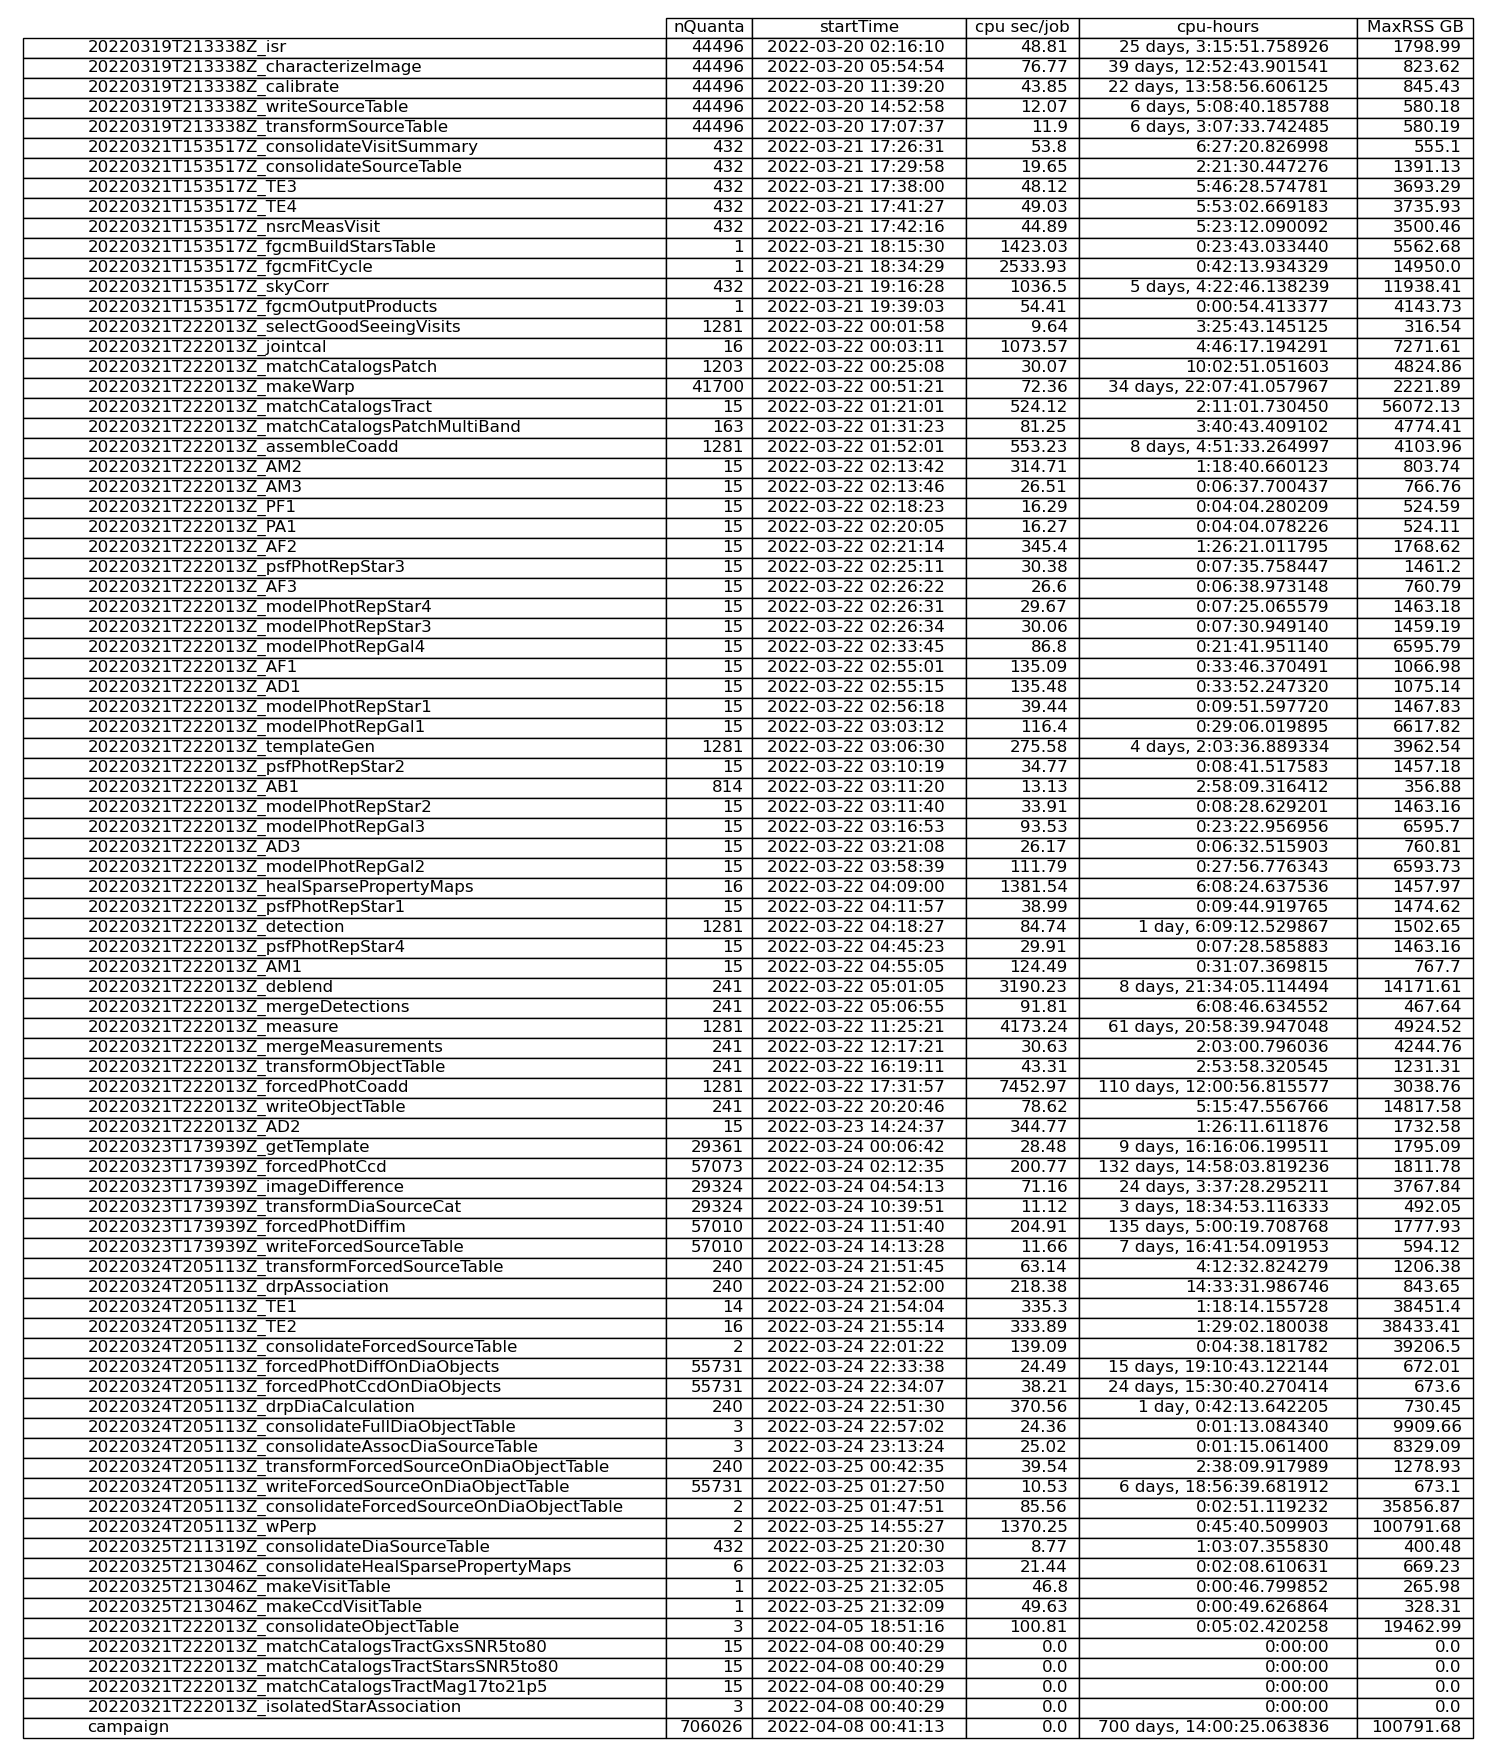
\includegraphics[width=5.96875in]{jira_imgs/2294.png}

}


\subsection{Test Cycle LVV-C162 }

Open test cycle {\it \href{https://jira.lsstcorp.org/secure/Tests.jspa#/testrun/LVV-C162}{LDM-503-GEN3: Gen 3 Ingest raw dataset}} in Jira.

Test Cycle name: LDM-503-GEN3: Gen 3 Ingest raw dataset\\
Status: Done

In the context of the milestone LDM-503-GEN3, Gen 3 Butler readiness,
this test cycle is defining the configuration and the dataset for
running a generic \textbf{Raw Data Ingestion Into Gen3 Butler} test
case. ~ There are currently 5 data sources that require verification as
they are the central products that will be produced by Rubin or are used
as precursor sets in the development/verification of the data management
software systems. ~The current raw data products that are deemed central
to DM development and testing are those from AuxTel/LATISS, ComCam, and
~precursor data from HyperSuprimeCam (HSC). ~Note, further tests using
LSSTCam (currently only preliminary BOT data from the SLAC test stand
are available) or precursor sets from the Dark Energy Camera (DECam)
could be added but since these types do not exactly fit the central
model used for LSST they are not tied directly to requirements.

\subsubsection{Software Version/Baseline}
LSST DM Stack with Gen3 Butler.

\subsubsection{Configuration}
Three separate raw data types, those from: AuxTel/LATISS, ComCam, and
HSC (e.g. a CI\_HSC raw) should be ingested when this test is executed.

\subsubsection{Test Cases in LVV-C162 Test Cycle}

\paragraph{ LVV-T1985 - Verify daf\_butler raw data ingest }\mbox{}\\

Version \textbf{1}.
Open  \href{https://jira.lsstcorp.org/secure/Tests.jspa#/testCase/LVV-T1985}{\textit{ LVV-T1985 } }
test case in Jira.

Demonstrate that a raw data type can be successfully ingested into a
Butler repository. ~

\textbf{ Preconditions}:\\
In order to run this test, a Gen3 daf butler should be deployed and
ready to use, with access to the filesystems where the raw data to
ingest is stored.

Execution status: {\bf Pass }

Final comment:\\The test can all be executed by running the script in the test plan and
report github repository: ~https://github.com/lsst-dm/\citeds{DMTR-271}/,
\citeds{DMTR-271}/scripts/LVV-T1985.sh on the lsst development machines at NCSA


Detailed steps results:

\begin{tabular}{p{2cm}p{14cm}}
\toprule
Step 1 & Step Execution Status: \textbf{ Pass } \\ \hline
\end{tabular}
 Description \\
{\footnotesize
Identify data for ingestion~{HSC RC2}⁠ and make ~a copy at a location
for the test. ~While a suggestion is provided in
{/project/shared/hsc/COSMOS/2014-03-27/}⁠ for a location where such data
can be found, the actual data used can be left to the discretion of the
person(s) executing the test with the added suggestion that relatively
recent data are more likely to reflect the current observatory system
state.\\[2\baselineskip]

}
\hdashrule[0.5ex]{\textwidth}{1pt}{3mm}
  Test Data \\
 {\footnotesize
{/project/shared/hsc/COSMOS/2014-03-27/}⁠~⁠~

}
\hdashrule[0.5ex]{\textwidth}{1pt}{3mm}
  Expected Result \\
{\footnotesize
One or more raw data sets are identified and made available.

}
\hdashrule[0.5ex]{\textwidth}{1pt}{3mm}
  Actual Result \\
{\footnotesize
The dataset identified for testing is
{/project/shared/hsc/COSMOS/2014-03-27/}‚Ā† ‚Ā†

}
\begin{tabular}{p{2cm}p{14cm}}
\toprule
Step 2 & Step Execution Status: \textbf{ Pass } \\ \hline
\end{tabular}
 Description \\
{\footnotesize
Identify data for ingestion~{AuxTel/LATISS}⁠ and make ~a copy at a
location for the test. ~While a suggestion is provided in
{/project/shared/auxTel/\_parent/raw/2022-04-06}⁠ for a location where
such data can be found, the actual data used can be left to the
discretion of the person(s) executing the test with the added suggestion
that relatively recent data are more likely to reflect the current
observatory system state.\\[2\baselineskip]

}
\hdashrule[0.5ex]{\textwidth}{1pt}{3mm}
  Test Data \\
 {\footnotesize
{/project/shared/auxTel/\_parent/raw/2022-04-06}⁠~⁠~

}
\hdashrule[0.5ex]{\textwidth}{1pt}{3mm}
  Expected Result \\
{\footnotesize
One or more raw data sets are identified and made available.

}
\hdashrule[0.5ex]{\textwidth}{1pt}{3mm}
  Actual Result \\
{\footnotesize
The dataset identified for testing is
/project/shared/auxTel/\_parent/raw/2022-04-06, which points to raw data
files at /lsstdata/offline/instrument/LATISS/storage/2022-04-06. A copy
was made to the directory used for this test. This dataset is kess than
one month old and contains calibration images and science images

}
\begin{tabular}{p{2cm}p{14cm}}
\toprule
Step 3 & Step Execution Status: \textbf{ Pass } \\ \hline
\end{tabular}
 Description \\
{\footnotesize
Identify data for ingestion~{ComCam}⁠ and make ~a copy at a location for
the test. ~While a suggestion is provided in
{/project/shared/comCam/\_parent/raw/2022-05-05/2022050500005}⁠ for a
location where such data can be found, the actual data used can be left
to the discretion of the person(s) executing the test with the added
suggestion that relatively recent data are more likely to reflect the
current observatory system state.\\[2\baselineskip]

}
\hdashrule[0.5ex]{\textwidth}{1pt}{3mm}
  Test Data \\
 {\footnotesize
{/project/shared/comCam/\_parent/raw/2022-05-05/2022050500005}⁠~⁠~

}
\hdashrule[0.5ex]{\textwidth}{1pt}{3mm}
  Expected Result \\
{\footnotesize
One or more raw data sets are identified and made available.

}
\hdashrule[0.5ex]{\textwidth}{1pt}{3mm}
  Actual Result \\
{\footnotesize
The dataset identified for testing is
~/project/shared/comCam/\_parent/raw/2022-05-05/202205050000005/ ⁠\\
, which points to raw data files at ~
/lsstdata/offline/instrument/LSSTComCam/storage/20220505/000005/. A copy
was made to the directory used for this test. This dataset is less than
one month old and contains calibration images and science images

}
\begin{tabular}{p{2cm}p{14cm}}
\toprule
Step 4 & Step Execution Status: \textbf{ Pass } \\ \hline
\end{tabular}
 Description \\
{\footnotesize
Create or identify an existing Butler repository for testing. If a
repository as already been created for a dataset used in this test,
reuse that repository.~

}
\hdashrule[0.5ex]{\textwidth}{1pt}{3mm}
  Example Code \\
{\footnotesize
\# Create empty Gen3 repo\\
butler create repo\\
butler config-dump repo --file repo.config

}
\hdashrule[0.5ex]{\textwidth}{1pt}{3mm}
  Expected Result \\
{\footnotesize

}
\hdashrule[0.5ex]{\textwidth}{1pt}{3mm}
  Actual Result \\
{\footnotesize
repository created and configuration file dumped~

}
\begin{tabular}{p{2cm}p{14cm}}
\toprule
Step 5 & Step Execution Status: \textbf{ Pass } \\ \hline
\end{tabular}
 Description \\
{\footnotesize
Create or identify an existing Butler repository for testing. If a
repository as already been created for a dataset used in this test,
reuse that repository.~

}
\hdashrule[0.5ex]{\textwidth}{1pt}{3mm}
  Example Code \\
{\footnotesize
\# Create empty Gen3 repo\\
butler create repo\\
butler config-dump repo --file repo.config

}
\hdashrule[0.5ex]{\textwidth}{1pt}{3mm}
  Expected Result \\
{\footnotesize

}
\hdashrule[0.5ex]{\textwidth}{1pt}{3mm}
  Actual Result \\
{\footnotesize
The repository~ created in the preious step was used for this instrument
as well.

}
\begin{tabular}{p{2cm}p{14cm}}
\toprule
Step 6 & Step Execution Status: \textbf{ Pass } \\ \hline
\end{tabular}
 Description \\
{\footnotesize
Create or identify an existing Butler repository for testing. If a
repository as already been created for a dataset used in this test,
reuse that repository.~

}
\hdashrule[0.5ex]{\textwidth}{1pt}{3mm}
  Example Code \\
{\footnotesize
\# Create empty Gen3 repo\\
butler create repo\\
butler config-dump repo --file repo.config

}
\hdashrule[0.5ex]{\textwidth}{1pt}{3mm}
  Expected Result \\
{\footnotesize

}
\hdashrule[0.5ex]{\textwidth}{1pt}{3mm}
  Actual Result \\
{\footnotesize
The repository created in the preious step was used for this instrument
as well.

}
\begin{tabular}{p{2cm}p{14cm}}
\toprule
Step 7 & Step Execution Status: \textbf{ Pass } \\ \hline
\end{tabular}
 Description \\
{\footnotesize
Verify that Butler repository is available for the {HSC RC2}⁠ (Note this
needs to be a test repository rather than the central repository as the
raw data should not already be present in the repository for this test.)

}
\hdashrule[0.5ex]{\textwidth}{1pt}{3mm}
  Test Data \\
 {\footnotesize
{url 1}⁠~

}
\hdashrule[0.5ex]{\textwidth}{1pt}{3mm}
  Example Code \\
{\footnotesize
butler register-instrument repo \textless{}instrument\textgreater{}\\
butler write-curated-calibrations repo
\textless{}instrument\textgreater{}\\[2\baselineskip]\# Check the
outputs\\
butler query-dimenstion-records repo instrument\\
butler query-collections~ repo --chains=tree

}
\hdashrule[0.5ex]{\textwidth}{1pt}{3mm}
  Expected Result \\
{\footnotesize

}
\hdashrule[0.5ex]{\textwidth}{1pt}{3mm}
  Actual Result \\
{\footnotesize
\textgreater{} butler query-dimension-records repo
instrument\\[2\baselineskip]name visit\_max exposure\_max detector\_max
class\_name\\
---- --------- ------------ ------------
-------------------------------\\
HSC 21474800 21474800 200
lsst.obs.subaru.HyperSuprimeCam\\[3\baselineskip]\textgreater{} butler
query-collections repo--chains=tree\\
\hspace*{0.333em} ~ ~ ~ ~ ~ ~ ~Name ~ ~ ~ ~ ~ ~ ~ ~ ~ ~Type ~\\
---------------------------------- -----------\\
HSC/calib CALIBRATION\\
HSC/calib/curated/19700101T000000Z RUN\\
HSC/calib/curated/20130131T000000Z RUN\\
HSC/calib/curated/20140403T000000Z RUN\\
HSC/calib/curated/20140601T000000Z RUN\\
HSC/calib/curated/20151106T000000Z RUN\\
HSC/calib/curated/20160401T000000Z RUN\\
HSC/calib/curated/20161122T000000Z RUN\\
HSC/calib/curated/20161223T000000Z RUN\\
HSC/calib/unbounded RUN\\[5\baselineskip]

}
\begin{tabular}{p{2cm}p{14cm}}
\toprule
Step 8 & Step Execution Status: \textbf{ Pass } \\ \hline
\end{tabular}
 Description \\
{\footnotesize
Verify that Butler repository is available for the {AuxTel/LATISS}⁠
(Note this needs to be a test repository rather than the central
repository as the raw data should not already be present in the
repository for this test.)

}
\hdashrule[0.5ex]{\textwidth}{1pt}{3mm}
  Test Data \\
 {\footnotesize
{url 2}⁠~

}
\hdashrule[0.5ex]{\textwidth}{1pt}{3mm}
  Example Code \\
{\footnotesize
butler register-instrument repo \textless{}instrument\textgreater{}\\
butler write-curated-calibrations repo
\textless{}instrument\textgreater{}\\[2\baselineskip]\# Check the
outputs\\
butler query-dimenstion-records repo instrument\\
butler query-collections~ repo --chains=tree

}
\hdashrule[0.5ex]{\textwidth}{1pt}{3mm}
  Expected Result \\
{\footnotesize

}
\hdashrule[0.5ex]{\textwidth}{1pt}{3mm}
  Actual Result \\
{\footnotesize
butler create repo\\
butler register-instrument repo lsst.obs.lsst.Latiss\\
butler query-dimenstion-records repo instrument\\[2\baselineskip]name
visit\_max exposure\_max detector\_max class\_name\\
------ ------------- ------------- ------------ --------------------\\
LATISS 6050123199999 6050123199999 0 lsst.obs.lsst.Latiss\\
(lsst-scipipe) {[}lguy@lsst-devl03 repo{]}\$ butler register-instrument
\$REPO lsst.obs.lsst.Latiss\\[3\baselineskip]butler query-collections
repo --chains=tree\\[2\baselineskip]Name Type\\
------------------------------------- -----------\\
LATISS/calib CALIBRATION\\
LATISS/calib/curated/19700101T000000Z RUN\\
LATISS/calib/curated/20180101T000000Z RUN\\
LATISS/calib/unbounded RUN\\[2\baselineskip]Check that both curated and
unbounded calibration collections are created

}
\begin{tabular}{p{2cm}p{14cm}}
\toprule
Step 9 & Step Execution Status: \textbf{ Pass } \\ \hline
\end{tabular}
 Description \\
{\footnotesize
Verify that Butler repository is available for the {ComCam}⁠ (Note this
needs to be a test repository rather than the central repository as the
raw data should not already be present in the repository for this test.)

}
\hdashrule[0.5ex]{\textwidth}{1pt}{3mm}
  Test Data \\
 {\footnotesize
{url 3}⁠~

}
\hdashrule[0.5ex]{\textwidth}{1pt}{3mm}
  Example Code \\
{\footnotesize
butler register-instrument repo \textless{}instrument\textgreater{}\\
butler write-curated-calibrations repo
\textless{}instrument\textgreater{}\\[2\baselineskip]\# Check the
outputs\\
butler query-dimenstion-records repo instrument\\
butler query-collections~ repo --chains=tree

}
\hdashrule[0.5ex]{\textwidth}{1pt}{3mm}
  Expected Result \\
{\footnotesize

}
\hdashrule[0.5ex]{\textwidth}{1pt}{3mm}
  Actual Result \\
{\footnotesize
\textgreater{} butler create repo\\
\textgreater{} butler register-instrument lsst.obs.lsst.LsstComCam\\
\textgreater{} butler write-curated-calibrations repo
lsst.obs.lsst.LsstComCam\\[2\baselineskip]\textgreater{} buter
query-dimension-records repo lsst.obs.lsst.LsstComCam\\
name visit\_max exposure\_max detector\_max class\_name\\
---------- ------------- ------------- ------------
------------------------\\
LSSTComCam 6050123199999 6050123199999 1000
lsst.obs.lsst.LsstComCam\\[2\baselineskip]\textgreater{} butler
query-collections repo --chains=tree\\
\hspace*{0.333em} ~ ~ ~ ~ ~Name ~ ~ ~ ~ ~ ~ ~ ~Type ~\\
-------------------------- -----------\\
LSSTComCam/calib CALIBRATION\\
LSSTComCam/calib/unbounded RUN

}
\begin{tabular}{p{2cm}p{14cm}}
\toprule
Step 10 & Step Execution Status: \textbf{ Pass } \\ \hline
\end{tabular}
 Description \\
{\footnotesize
Ingest {HSC RC2}⁠~raw data into repo

}
\hdashrule[0.5ex]{\textwidth}{1pt}{3mm}
  Test Data \\
 {\footnotesize
{url 1}⁠~

}
\hdashrule[0.5ex]{\textwidth}{1pt}{3mm}
  Example Code \\
{\footnotesize
butler ingest-raws repo /path/to/raw/fitsfiles

}
\hdashrule[0.5ex]{\textwidth}{1pt}{3mm}
  Expected Result \\
{\footnotesize
Tool reports data ingest successful for {HSC RC2}⁠ into {url 1}⁠~

}
\hdashrule[0.5ex]{\textwidth}{1pt}{3mm}
  Actual Result \\
{\footnotesize
\textgreater{} butler ingest-raws repo /path/to/raws --transfer
link\\[2\baselineskip]lsst.ingest INFO: Successfully extracted metadata
from 4144 files with 0 failures\\
lsst.ingest INFO: Exposure HSC:HSCA00088200 ingested successfully\\
\ldots{}\ldots{}\\
lsst.ingest INFO: Successfully processed data from 37 exposures with 0
failures from exposure registration and 0 failures from file ingest.\\
lsst.ingest INFO: Ingested 4144 distinct Butler datasets

}
\begin{tabular}{p{2cm}p{14cm}}
\toprule
Step 11 & Step Execution Status: \textbf{ Pass } \\ \hline
\end{tabular}
 Description \\
{\footnotesize
Ingest {AuxTel/LATISS}⁠~raw data into repo

}
\hdashrule[0.5ex]{\textwidth}{1pt}{3mm}
  Test Data \\
 {\footnotesize
{url 2}⁠~

}
\hdashrule[0.5ex]{\textwidth}{1pt}{3mm}
  Example Code \\
{\footnotesize
butler ingest-raws repo /path/to/raw/fitsfiles

}
\hdashrule[0.5ex]{\textwidth}{1pt}{3mm}
  Expected Result \\
{\footnotesize
Tool reports data ingest successful for {AuxTel/LATISS}⁠ into {url 2}⁠~

}
\hdashrule[0.5ex]{\textwidth}{1pt}{3mm}
  Actual Result \\
{\footnotesize
\textgreater{} butler ingest-raws repo /path/to/raw/fits
--transfer=link\\[2\baselineskip]lsst.ingest INFO: Successfully
extracted metadata from 1126 files with 0 failures\\
lsst.ingest INFO: Exposure LATISS:AT\_O\_20220406\_001090 ingested
successfully\\
\ldots{}\ldots{}\ldots{}.\\
lsst.ingest INFO: Exposure LATISS:AT\_O\_20220406\_000108 ingested
successfully\\
lsst.ingest INFO: Successfully processed data from 1126 exposures with 0
failures from exposure registration and 0 failures from file ingest.\\
lsst.ingest INFO: Ingested 1126 distinct Butler
datasets\\[2\baselineskip]No errors were reported in the ingest process

}
\begin{tabular}{p{2cm}p{14cm}}
\toprule
Step 12 & Step Execution Status: \textbf{ Pass } \\ \hline
\end{tabular}
 Description \\
{\footnotesize
Ingest {ComCam}⁠~raw data into repo

}
\hdashrule[0.5ex]{\textwidth}{1pt}{3mm}
  Test Data \\
 {\footnotesize
{url 3}⁠~

}
\hdashrule[0.5ex]{\textwidth}{1pt}{3mm}
  Example Code \\
{\footnotesize
butler ingest-raws repo /path/to/raw/fitsfiles

}
\hdashrule[0.5ex]{\textwidth}{1pt}{3mm}
  Expected Result \\
{\footnotesize
Tool reports data ingest successful for {ComCam}⁠ into {url 3}⁠~

}
\hdashrule[0.5ex]{\textwidth}{1pt}{3mm}
  Actual Result \\
{\footnotesize
\textgreater{} butler ingest-raws repo /path/to/raw/fitsfiles
--transfer=link\\[2\baselineskip]lsst.ingest INFO: Successfully
extracted metadata from 9 files with 0 failures\\
lsst.ingest INFO: Exposure LSSTComCam:CC\_O\_20220505\_000005 ingested
successfully\\
lsst.ingest INFO: Successfully processed data from 1 exposure with 0
failures from exposure registration and 0 failures from file ingest.\\
lsst.ingest INFO: Ingested 9 distinct Butler datasets

}
\begin{tabular}{p{2cm}p{14cm}}
\toprule
Step 13 & Step Execution Status: \textbf{ Pass } \\ \hline
\end{tabular}
 Description \\
{\footnotesize
Query repository to verify that ingestion of {HSC RC2}⁠~ occurred.

}
\hdashrule[0.5ex]{\textwidth}{1pt}{3mm}
  Test Data \\
 {\footnotesize
{url 1}⁠~

}
\hdashrule[0.5ex]{\textwidth}{1pt}{3mm}
  Example Code \\
{\footnotesize
\begin{verbatim}
butler query-collections repo --chains=tree
\end{verbatim}

\begin{verbatim}
butler query-dimension-records repo exposure
\end{verbatim}

}
\hdashrule[0.5ex]{\textwidth}{1pt}{3mm}
  Expected Result \\
{\footnotesize
{HSC RC2}⁠ data are found by query.~

}
\hdashrule[0.5ex]{\textwidth}{1pt}{3mm}
  Actual Result \\
{\footnotesize
\textgreater{}~

\begin{verbatim}
butler query-collections repo --chains=tree
\end{verbatim}

Name Type\\
---------------------------------- -----------\\
HSC/calib CALIBRATION\\
HSC/calib/curated/19700101T000000Z RUN\\
HSC/calib/curated/20130131T000000Z RUN\\
HSC/calib/curated/20140403T000000Z RUN\\
HSC/calib/curated/20140601T000000Z RUN\\
HSC/calib/curated/20151106T000000Z RUN\\
HSC/calib/curated/20160401T000000Z RUN\\
HSC/calib/curated/20161122T000000Z RUN\\
HSC/calib/curated/20161223T000000Z RUN\\
HSC/calib/unbounded RUN\\
HSC/raw/all RUN\\[2\baselineskip]The HSC/raw/all and HSC/calib
collections exist\\[2\baselineskip]

\begin{verbatim}
> butler query-dimension-records repo exposure
\end{verbatim}

instrument id physical\_filter obs\_id exposure\_time dark\_time
observation\_type observation\_reason day\_obs seq\_num group\_name
group\_id target\_name science\_program tracking\_ra tracking\_dec
sky\_angle zenith\_angle timespan {[}2{]}\\
---------- --- --------------- ------------ -----------------
----------------- ---------------- ------------------ -------- -------
---------- -------- ----------- --------------- ------------------
------------------ --------- ------------------
--------------------------------------------------------\\
HSC 872 HSC-I HSCA00087200 30.0 30.0 science science 20140327 872 872
872 COSMOS o14311 150.11877083333331 2.205855555555556 180.0 23.8768551
2014-03-27 06:59:34.970000 .. 2014-03-27
07:00:07.037000\\[2\baselineskip]\ldots{}.

}
\begin{tabular}{p{2cm}p{14cm}}
\toprule
Step 14 & Step Execution Status: \textbf{ Pass } \\ \hline
\end{tabular}
 Description \\
{\footnotesize
Query repository to verify that ingestion of {AuxTel/LATISS}⁠~ occurred.

}
\hdashrule[0.5ex]{\textwidth}{1pt}{3mm}
  Test Data \\
 {\footnotesize
{url 2}⁠~

}
\hdashrule[0.5ex]{\textwidth}{1pt}{3mm}
  Example Code \\
{\footnotesize
\begin{verbatim}
butler query-collections repo --chains=tree
\end{verbatim}

\begin{verbatim}
butler query-dimension-records repo exposure
\end{verbatim}

}
\hdashrule[0.5ex]{\textwidth}{1pt}{3mm}
  Expected Result \\
{\footnotesize
{AuxTel/LATISS}⁠ data are found by query.~

}
\hdashrule[0.5ex]{\textwidth}{1pt}{3mm}
  Actual Result \\
{\footnotesize
\textgreater{} butler query-collections \$REPO --chains=tree\\
Name Type\\
------------------------------------- -----------\\
LATISS/calib CALIBRATION\\
LATISS/calib/curated/19700101T000000Z RUN\\
LATISS/calib/curated/20180101T000000Z RUN\\
LATISS/calib/unbounded RUN\\
LATISS/raw/all RUN\\[2\baselineskip]Check that ingesting the images has
createsd a the ``all'' collection

}
\begin{tabular}{p{2cm}p{14cm}}
\toprule
Step 15 & Step Execution Status: \textbf{ Pass } \\ \hline
\end{tabular}
 Description \\
{\footnotesize
Query repository to verify that ingestion of {ComCam}⁠~ occurred.

}
\hdashrule[0.5ex]{\textwidth}{1pt}{3mm}
  Test Data \\
 {\footnotesize
{url 3}⁠~

}
\hdashrule[0.5ex]{\textwidth}{1pt}{3mm}
  Example Code \\
{\footnotesize
\begin{verbatim}
butler query-collections repo --chains=tree
\end{verbatim}

\begin{verbatim}
butler query-dimension-records repo exposure
\end{verbatim}

}
\hdashrule[0.5ex]{\textwidth}{1pt}{3mm}
  Expected Result \\
{\footnotesize
{ComCam}⁠ data are found by query.~

}
\hdashrule[0.5ex]{\textwidth}{1pt}{3mm}
  Actual Result \\
{\footnotesize
\textgreater{} butler query-collections repo
--chains=tree\\[2\baselineskip]Name Type\\
-------------------------- -----------\\
LSSTComCam/calib CALIBRATION\\
LSSTComCam/calib/unbounded RUN\\
LSSTComCam/raw/all RUN\\[2\baselineskip]The LSSTComCam/raw/all
collection has been created\\[2\baselineskip]\textgreater{} butler
query-dimension-records \$REPO exposure --where
``instrument='LSSTComCam' AND
exposure.observation\_type='bias'''\\[2\baselineskip]instrument id
physical\_filter obs\_id exposure\_time dark\_time observation\_type
observation\_reason day\_obs seq\_num group\_name group\_id target\_name
science\_program tracking\_ra tracking\_dec sky\_angle zenith\_angle
timespan {[}2{]}\\
---------- ------------- --------------- --------------------
------------- --------- ---------------- ------------------ --------
------- ---------- ------------------- ----------- ---------------
----------- ------------ --------- ------------
--------------------------------------------------------\\
LSSTComCam 2022050500005 i\_06 CC\_O\_20220505\_000005 5.0 6.15436 bias
unknown 20220505 5 g 6221118600778448001 UNKNOWN unknown None None None
None 2022-05-05 19:04:23.719980 .. 2022-05-05
19:04:29.813000\\[2\baselineskip]\# There are no science images in this
dataset\\
\textgreater{} butler query-dimension-records \$REPO exposure --where
``instrument='LSSTComCam' AND exposure.observation\_type='science'''\\
No results. Try --help for more information.

}


\subsection{Test Cycle LVV-C190 }

Open test cycle {\it \href{https://jira.lsstcorp.org/secure/Tests.jspa#/testrun/LVV-C190}{\citeds{LDM-556}: Middleware Acceptance Testing}} in Jira.

Test Cycle name: \citeds{LDM-556}: Middleware Acceptance Testing\\
Status: In Progress



\subsubsection{Software Version/Baseline}
Not provided.

\subsubsection{Configuration}
Not provided.

\subsubsection{Test Cases in LVV-C190 Test Cycle}

\paragraph{ LVV-T2503 - Verify Outputs from Test Processing Runs }\mbox{}\\

Version \textbf{1}.
Open  \href{https://jira.lsstcorp.org/secure/Tests.jspa#/testCase/LVV-T2503}{\textit{ LVV-T2503 } }
test case in Jira.

Verify that the Data Output System interface is usable by algorithmic
code being run for test/development purposes, on both development
compute environments at the archive center and in personal environments.

\textbf{ Preconditions}:\\


Execution status: {\bf Pass }

Final comment:\\


Detailed steps results:

\begin{tabular}{p{2cm}p{14cm}}
\toprule
Step 1 & Step Execution Status: \textbf{ Pass } \\ \hline
\end{tabular}
 Description \\
{\footnotesize
Demonstrated by regular reprocessing runs at NCSA.

}
\hdashrule[0.5ex]{\textwidth}{1pt}{3mm}
  Expected Result \\
{\footnotesize

}
\hdashrule[0.5ex]{\textwidth}{1pt}{3mm}
  Actual Result \\
{\footnotesize
This capability is demonstrated by the regular monthly (re-)processing
of the RC2 dataset. The most recent processing was executed with weekly
release `w\_2022\_12` on the NCSA lsst-devl machines; details can be
found in Jira ticket DM-34125.\\[2\baselineskip]Data quality metrics
measured on these data appear on April 14 in the following screenshot
from our metric monitoring dashboard:\\
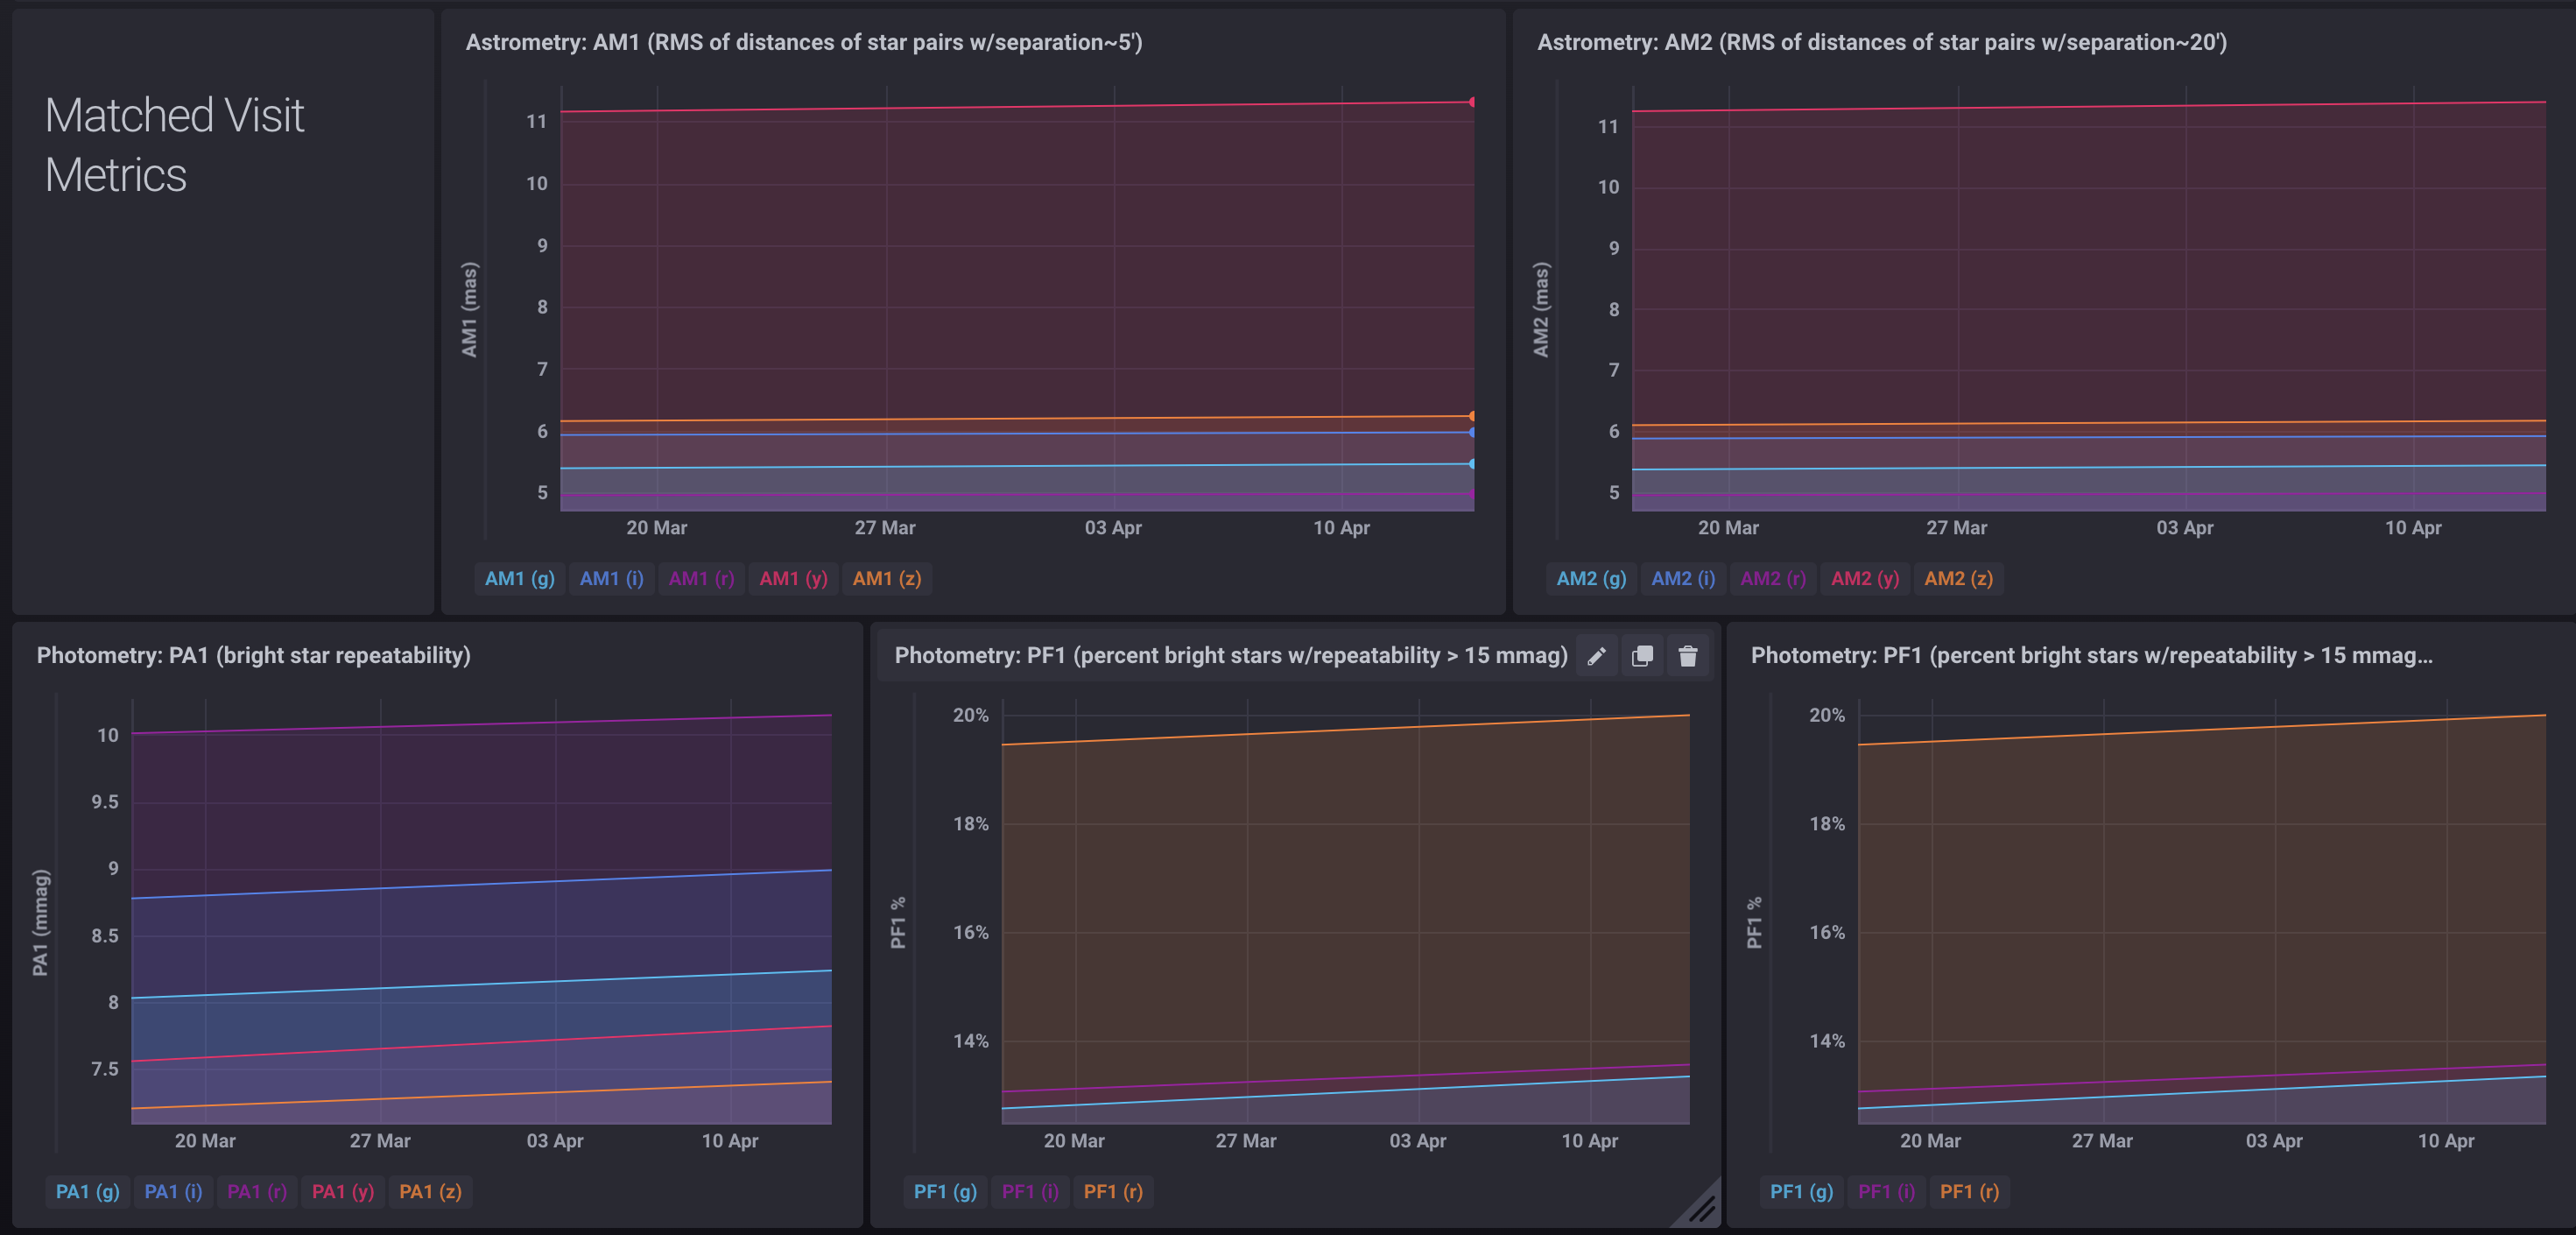
\includegraphics[width=5.63542in]{jira_imgs/2343.png}

}

\paragraph{ LVV-T2502 - Verify Outputs from Science Platform }\mbox{}\\

Version \textbf{1}.
Open  \href{https://jira.lsstcorp.org/secure/Tests.jspa#/testCase/LVV-T2502}{\textit{ LVV-T2502 } }
test case in Jira.

Verify that the ~Data Output System interface shall be usable by
algorithmic code run in the Science Platform

\textbf{ Preconditions}:\\


Execution status: {\bf Pass }

Final comment:\\


Detailed steps results:

\begin{tabular}{p{2cm}p{14cm}}
\toprule
Step 1 & Step Execution Status: \textbf{ Pass } \\ \hline
\end{tabular}
 Description \\
{\footnotesize
Demonstrated by any Science Platform notebook that uses the butler.

}
\hdashrule[0.5ex]{\textwidth}{1pt}{3mm}
  Expected Result \\
{\footnotesize

}
\hdashrule[0.5ex]{\textwidth}{1pt}{3mm}
  Actual Result \\
{\footnotesize
On the Science Platform at
\href{http://data.lsst.cloud}{data.lsst.cloud}, execute the Data Preview
0 tutorial notebook
"\href{https://github.com/rubin-dp0/tutorial-notebooks/blob/main/04_Intro_to_Butler.ipynb}{Intro
to Butler}". This notebook gives a guided tour of the butler and its
capabilities, using the Data Preview 0.1 data available at the Interim
Data Facility. A screenshot of a small portion of this notebook is shown
below:\\[2\baselineskip]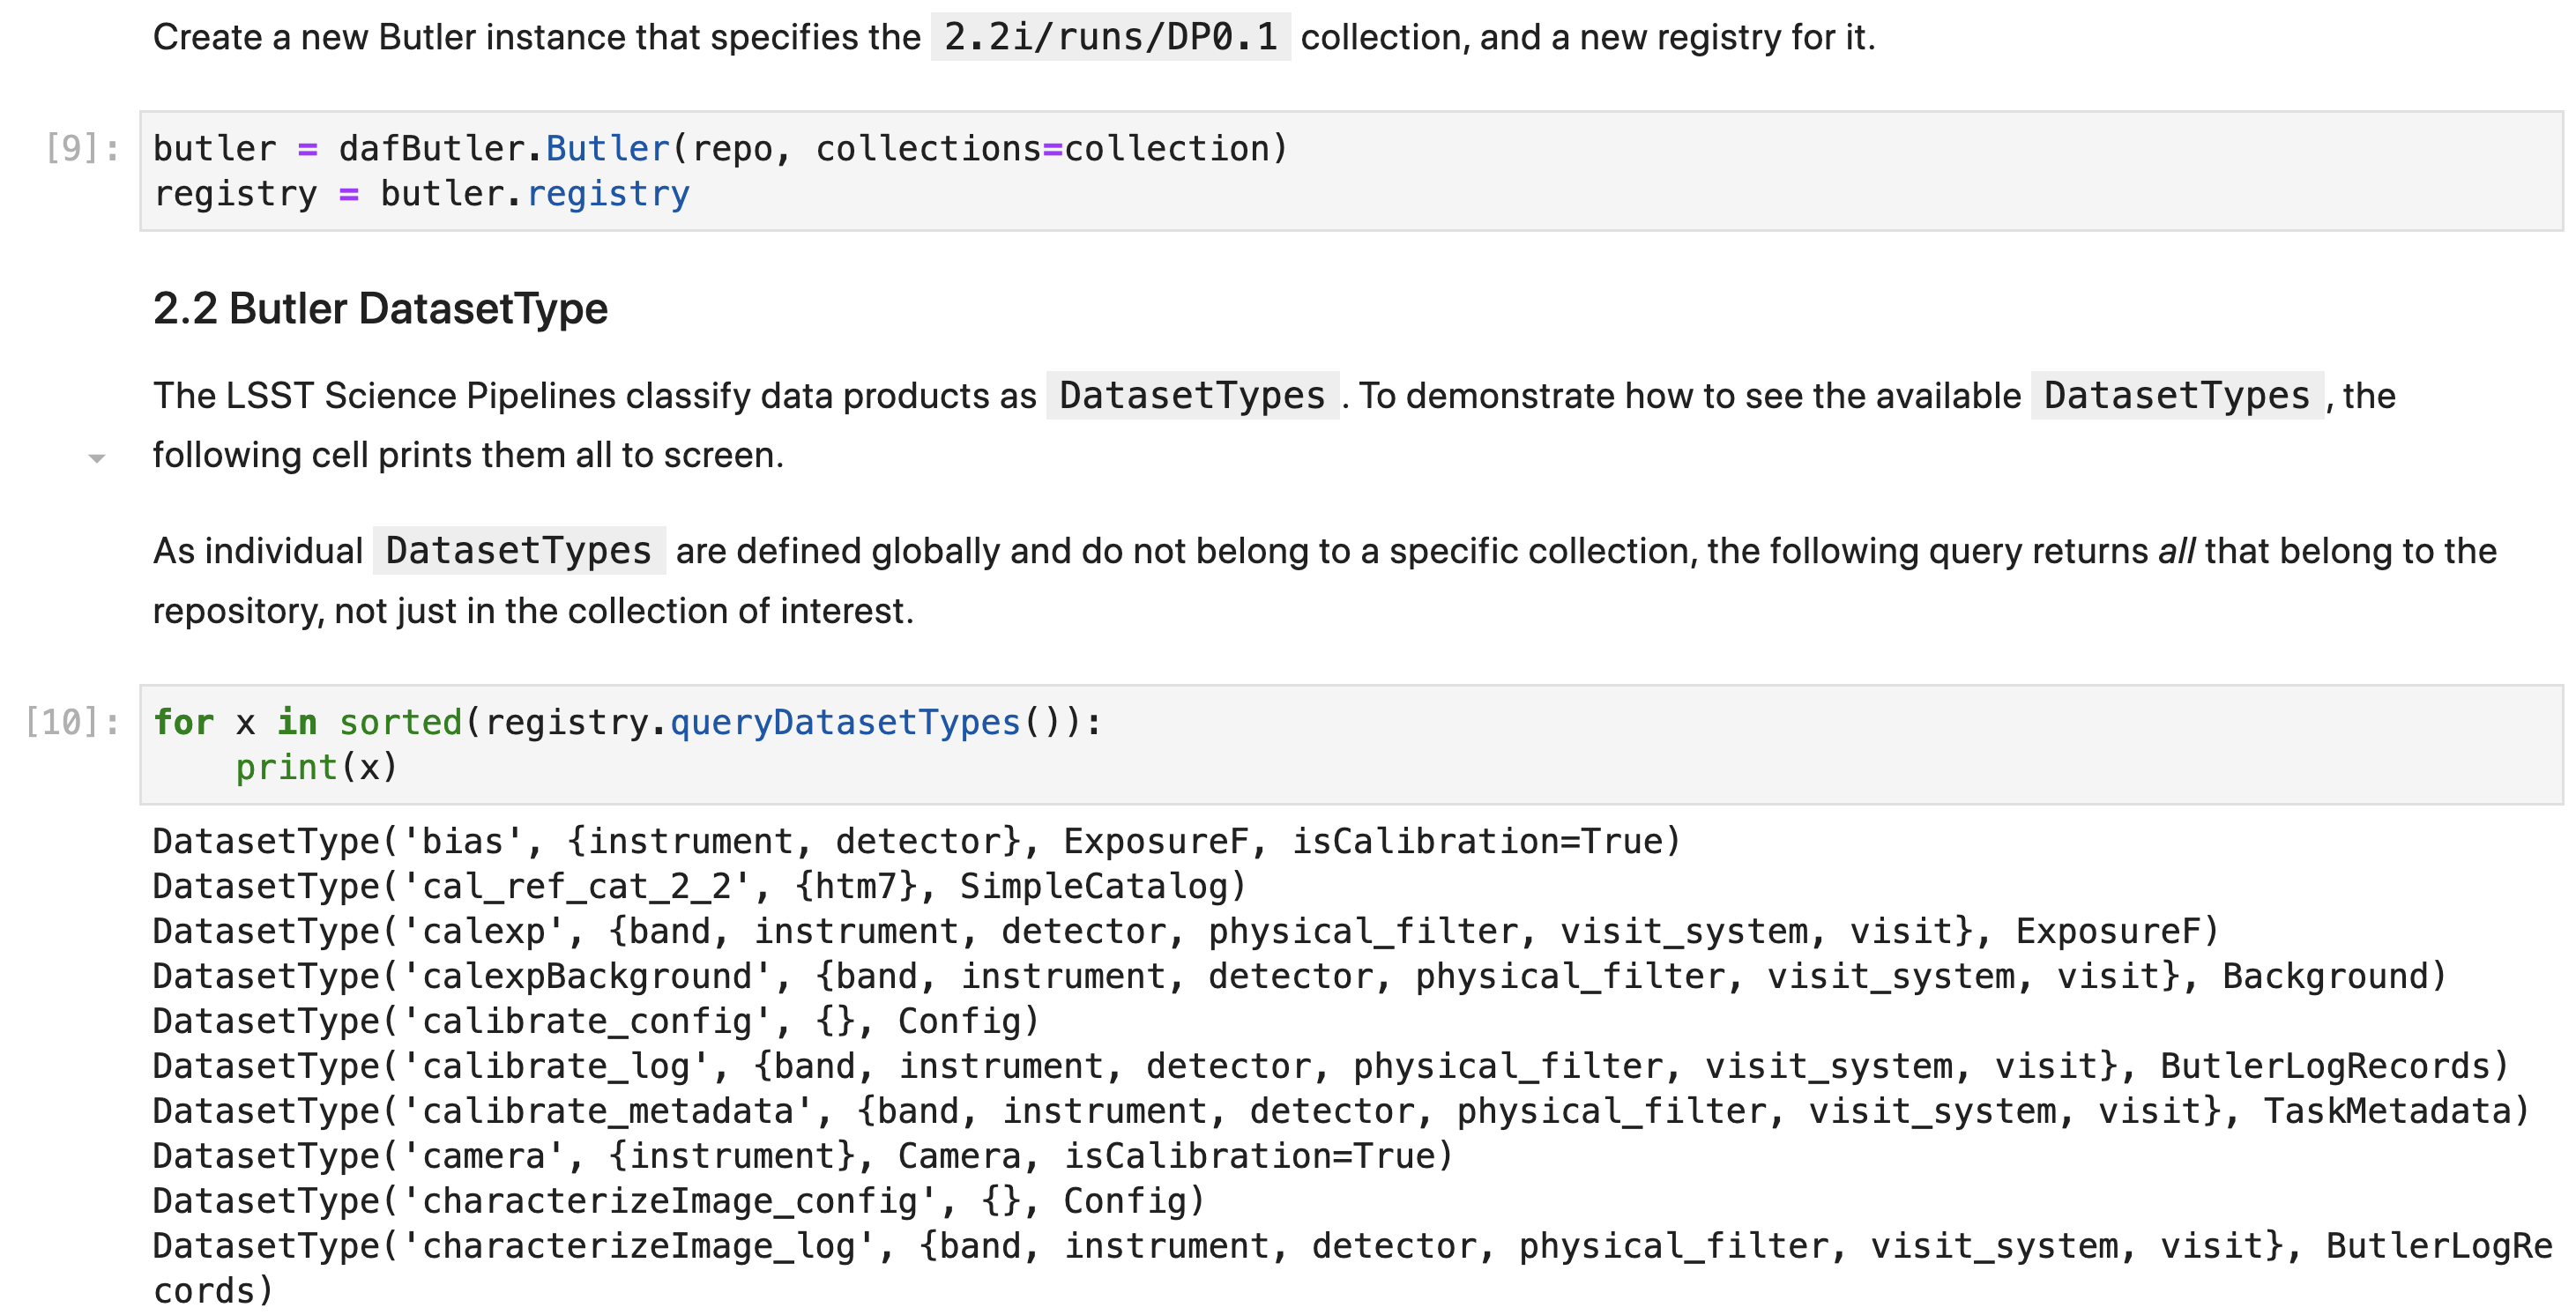
\includegraphics[width=6.07292in]{jira_imgs/2350.png}

}

\paragraph{ LVV-T2501 - Verify Outputs from Data Release Production }\mbox{}\\

Version \textbf{1}.
Open  \href{https://jira.lsstcorp.org/secure/Tests.jspa#/testCase/LVV-T2501}{\textit{ LVV-T2501 } }
test case in Jira.

Verify that the Data Output System interface is usable by algorithmic
code being run as part of Data Release
Production.\\[2\baselineskip]Demonstrated by regular reprocessing runs
at NCSA and DP0.2 production.

\textbf{ Preconditions}:\\


Execution status: {\bf Not Executed }

Final comment:\\


Detailed steps results:

\begin{tabular}{p{2cm}p{14cm}}
\toprule
Step 1 & Step Execution Status: \textbf{ Not Executed } \\ \hline
\end{tabular}
 Description \\
{\footnotesize

}
\hdashrule[0.5ex]{\textwidth}{1pt}{3mm}
  Expected Result \\
{\footnotesize

}
\hdashrule[0.5ex]{\textwidth}{1pt}{3mm}
  Actual Result \\
{\footnotesize

}

\paragraph{ LVV-T2499 - Verify Consistent Output Interface }\mbox{}\\

Version \textbf{1}.
Open  \href{https://jira.lsstcorp.org/secure/Tests.jspa#/testCase/LVV-T2499}{\textit{ LVV-T2499 } }
test case in Jira.

Verify that the ~Data Output System ~provides a consistent interface for
writing InMemoryDatasets to storage given a DatasetRef across different
types of DataRepositories.

\textbf{ Preconditions}:\\


Execution status: {\bf Pass }

Final comment:\\


Detailed steps results:

\begin{tabular}{p{2cm}p{14cm}}
\toprule
Step 1 & Step Execution Status: \textbf{ Pass } \\ \hline
\end{tabular}
 Description \\
{\footnotesize
Execute the unit tests at
https://github.com/lsst/daf\_butler/blob/main/tests/test\_butler.py --
in particular, the tests that exercise ImportExport or PutGet in repos
on different types of datastores.

}
\hdashrule[0.5ex]{\textwidth}{1pt}{3mm}
  Expected Result \\
{\footnotesize
Unit tests pass.

}
\hdashrule[0.5ex]{\textwidth}{1pt}{3mm}
  Actual Result \\
{\footnotesize
Working with a cloned `daf\_butler` repository at
/project/jcarlin/SVV/gen3\_middleware\_acceptance\_testing/daf\_butler
on the lsst-devl machines.\\[2\baselineskip]Executed the unit test via:
``pytest -s -vv --no-header
tests/test\_butler.py''\\[2\baselineskip]Among the results, these are
the relevant
tests:\\[2\baselineskip]tests/test\_butler.py::ButlerConfigTests::testSearchPath
PASSED\\
tests/test\_butler.py::PosixDatastoreButlerTestCase::testBasicPutGet
PASSED\\
tests/test\_butler.py::PosixDatastoreButlerTestCase::testButlerRewriteDataId
PASSED\\
tests/test\_butler.py::PosixDatastoreButlerTestCase::testCompositePutGetConcrete
PASSED\\
tests/test\_butler.py::PosixDatastoreButlerTestCase::testCompositePutGetVirtual
PASSED\\
tests/test\_butler.py::PosixDatastoreButlerTestCase::testExportTransferCopy
PASSED\\
tests/test\_butler.py::PosixDatastoreButlerTestCase::testImportExport
Root:
file:///project/jcarlin/SVV/gen3\_middleware\_acceptance\_testing/daf\_butler/tests/tmpfsk\_pyeg/\\
PASSED\\
tests/test\_butler.py::PosixDatastoreButlerTestCase::testIngest PASSED\\
tests/test\_butler.py::PosixDatastoreButlerTestCase::testPutTemplates
PASSED\\[2\baselineskip]tests/test\_butler.py::InMemoryDatastoreButlerTestCase::testBasicPutGet
PASSED\\
tests/test\_butler.py::InMemoryDatastoreButlerTestCase::testButlerRewriteDataId
PASSED\\
tests/test\_butler.py::InMemoryDatastoreButlerTestCase::testCompositePutGetConcrete
PASSED\\
tests/test\_butler.py::InMemoryDatastoreButlerTestCase::testCompositePutGetVirtual
PASSED\\[2\baselineskip]tests/test\_butler.py::ChainedDatastoreButlerTestCase::testBasicPutGet
PASSED\\
tests/test\_butler.py::ChainedDatastoreButlerTestCase::testButlerRewriteDataId
PASSED\\
tests/test\_butler.py::ChainedDatastoreButlerTestCase::testCompositePutGetConcrete
PASSED\\
tests/test\_butler.py::ChainedDatastoreButlerTestCase::testCompositePutGetVirtual
PASSED\\[2\baselineskip]tests/test\_butler.py::ButlerExplicitRootTestCase::testBasicPutGet
PASSED\\
tests/test\_butler.py::ButlerExplicitRootTestCase::testButlerRewriteDataId
PASSED\\
tests/test\_butler.py::ButlerExplicitRootTestCase::testCompositePutGetConcrete
PASSED\\
tests/test\_butler.py::ButlerExplicitRootTestCase::testCompositePutGetVirtual
PASSED\\
tests/test\_butler.py::ButlerExplicitRootTestCase::testExportTransferCopy
PASSED\\
tests/test\_butler.py::ButlerExplicitRootTestCase::testImportExport
Root:
file:///project/jcarlin/SVV/gen3\_middleware\_acceptance\_testing/daf\_butler/tests/tmpvehpotd7/dir1/\\
PASSED\\[2\baselineskip]tests/test\_butler.py::ButlerMakeRepoOutfileTestCase::testConfigExistence
PASSED\\
tests/test\_butler.py::ButlerMakeRepoOutfileTestCase::testDeferredCollectionPassing
PASSED\\
tests/test\_butler.py::ButlerMakeRepoOutfileTestCase::testPutGet
PASSED\\
tests/test\_butler.py::ButlerMakeRepoOutfileDirTestCase::testConfigExistence
PASSED\\
tests/test\_butler.py::ButlerMakeRepoOutfileDirTestCase::testDeferredCollectionPassing
PASSED\\
tests/test\_butler.py::ButlerMakeRepoOutfileDirTestCase::testPutGet
PASSED\\
tests/test\_butler.py::ButlerMakeRepoOutfileUriTestCase::testConfigExistence
PASSED\\
tests/test\_butler.py::ButlerMakeRepoOutfileUriTestCase::testDeferredCollectionPassing
PASSED\\
tests/test\_butler.py::ButlerMakeRepoOutfileUriTestCase::testPutGet
PASSED\\
tests/test\_butler.py::S3DatastoreButlerTestCase::testBasicPutGet
PASSED\\
tests/test\_butler.py::S3DatastoreButlerTestCase::testButlerRewriteDataId
PASSED\\
tests/test\_butler.py::S3DatastoreButlerTestCase::testCompositePutGetConcrete
PASSED\\
tests/test\_butler.py::S3DatastoreButlerTestCase::testCompositePutGetVirtual
PASSED\\
tests/test\_butler.py::S3DatastoreButlerTestCase::testImportExport Root:
s3://anybucketname/CO0O55Y0EX8RB8X9EE5U/\\[2\baselineskip]All of these
unit tests have passed. We have thus demonstrated a consistent interface
for writing InMemoryDatasets to storage across different types of
repositories.

}

\paragraph{ LVV-T2498 - Verify Writing FITS tables }\mbox{}\\

Version \textbf{1}.
Open  \href{https://jira.lsstcorp.org/secure/Tests.jspa#/testCase/LVV-T2498}{\textit{ LVV-T2498 } }
test case in Jira.

Verify that the Data Output System is able to write in-memory table
objects as FITS files.

\textbf{ Preconditions}:\\


Execution status: {\bf Pass }

Final comment:\\


Detailed steps results:

\begin{tabular}{p{2cm}p{14cm}}
\toprule
Step 1 & Step Execution Status: \textbf{ Pass } \\ \hline
\end{tabular}
 Description \\
{\footnotesize
Execute unit tests ``test\_fitsTables.cc'' and ``test\_fits.py'' in
\href{https://github.com/lsst/afw}{lsst.afw} package.

}
\hdashrule[0.5ex]{\textwidth}{1pt}{3mm}
  Expected Result \\
{\footnotesize
Unit tests pass.

}
\hdashrule[0.5ex]{\textwidth}{1pt}{3mm}
  Actual Result \\
{\footnotesize
Executed `scons` in a cloned version of the `afw` package on lsst-devl
at NCSA. Here is the relevant line from the log indicating that the C++
unit tests in ``test\_fitsTables.cc'' passed:\\[2\baselineskip]running
tests/test\_fitsTables\ldots{} passed\\[2\baselineskip]Next, execute the
`test\_fits.py` unit test on its own:\\[2\baselineskip]pytest -s -vv
--no-header --cache-clear
tests/test\_fits.py\\[2\baselineskip]Results:\\[2\baselineskip]tests/test\_fits.py::FLAKE8
PASSED\\
tests/test\_fits.py::FitsTestCase::testIgnoreKeywords~PASSED\\
tests/test\_fits.py::FitsTestCase::testReadBlankKeywordComment~PASSED\\
tests/test\_fits.py::FitsTestCase::testReadUndefined lsst.afw.fits WARN:
In void
lsst::afw::fits::\{anonymous\}::MetadataIterationFunctor::add(const
string\&, const string\&), dropping undefined value for key `ADC-STR'.\\
lsst.afw.fits WARN: In void
lsst::afw::fits::\{anonymous\}::MetadataIterationFunctor::add(const
string\&, T, const string\&) {[}with T = double; std::string =
std::\_\_cxx11::basic\_string\textless{}char\textgreater{}{]}, replacing
undefined value for key `DOM-WND'.\\
PASSED\\
tests/test\_fits.py::FitsTestCase::testSimpleIO~PASSED\\
tests/test\_fits.py::FitsTestCase::testUndefinedVector~PASSED\\
tests/test\_fits.py::TestMemory::testFileDescriptorLeaks \textless{}-
../../../../../software/lsstsw/stack\_20220215/stack/miniconda3-py38\_4.9.2-2.0.0/Linux64/utils/g617c0b0dc2+9633a190c8/python/lsst/utils/tests.py
PASSED\\[2\baselineskip]Thus the writing of FITS tables has been
demonstrated.

}

\paragraph{ LVV-T2497 - Verify Writing FITS images }\mbox{}\\

Version \textbf{1}.
Open  \href{https://jira.lsstcorp.org/secure/Tests.jspa#/testCase/LVV-T2497}{\textit{ LVV-T2497 } }
test case in Jira.

Verify that the ~Data Output System is able to write in-memory image
objects as FITS files

\textbf{ Preconditions}:\\


Execution status: {\bf Pass }

Final comment:\\


Detailed steps results:

\begin{tabular}{p{2cm}p{14cm}}
\toprule
Step 1 & Step Execution Status: \textbf{ Pass } \\ \hline
\end{tabular}
 Description \\
{\footnotesize
Execute unit tests ``test\_imageIo1.py'' and ``test\_imageIo2.py'' in
\href{https://github.com/lsst/afw}{lsst.afw}~package.

}
\hdashrule[0.5ex]{\textwidth}{1pt}{3mm}
  Expected Result \\
{\footnotesize
Unit tests pass.

}
\hdashrule[0.5ex]{\textwidth}{1pt}{3mm}
  Actual Result \\
{\footnotesize
First, clone and set up the `afwdata` package:\\
git clone https://github.com/lsst/afwdata.git\\
cd afwdata\\
setup -j -r .\\[2\baselineskip]Now navigate to a cloned, set up
repository of `lsst.afw` on the lsst-devl machines at NCSA, and execute
the following:\\[2\baselineskip]pytest -s -vv --no-header --cache-clear
tests/test\_imageIo1.py\\[2\baselineskip]Results:\\
tests/test\_imageIo1.py::FLAKE8~PASSED\\
tests/test\_imageIo1.py::ReadFitsTestCase::testBBoxFromMetadata~PASSED\\
tests/test\_imageIo1.py::ReadFitsTestCase::testF32~PASSED\\
tests/test\_imageIo1.py::ReadFitsTestCase::testF64~PASSED\\
tests/test\_imageIo1.py::ReadFitsTestCase::testImageCompressionDisabled~PASSED\\
tests/test\_imageIo1.py::ReadFitsTestCase::testLongStrings~PASSED\\
tests/test\_imageIo1.py::ReadFitsTestCase::testMEF~PASSED\\
tests/test\_imageIo1.py::ReadFitsTestCase::testReadFitsWithOptions~PASSED\\
tests/test\_imageIo1.py::ReadFitsTestCase::testS16~PASSED\\
tests/test\_imageIo1.py::ReadFitsTestCase::testSubimage~PASSED\\
tests/test\_imageIo1.py::ReadFitsTestCase::testU16~PASSED\\
tests/test\_imageIo1.py::ReadFitsTestCase::testWriteBool~PASSED\\
tests/test\_imageIo1.py::ReadFitsTestCase::testWriteReadF64~PASSED\\
tests/test\_imageIo1.py::TestMemory::testFileDescriptorLeaks
\textless{}-
../../../../../software/lsstsw/stack\_20220215/stack/miniconda3-py38\_4.9.2-2.0.0/Linux64/utils/g617c0b0dc2+9633a190c8/python/lsst/utils/tests.py
PASSED\\[2\baselineskip]pytest -s -vv --no-header --cache-clear
tests/test\_imageIo2.py\\[2\baselineskip]Results:\\
tests/test\_imageIo2.py::FLAKE8~PASSED\\
tests/test\_imageIo2.py::ImageIoTestCase::testFloatCompressedLossless~PASSED\\
tests/test\_imageIo2.py::ImageIoTestCase::testFloatCompressedManual~SKIPPED~(Fix
deferred to DM-15644)\\
tests/test\_imageIo2.py::ImageIoTestCase::testFloatCompressedRange~SKIPPED~(Fix
deferred to DM-15644)\\
tests/test\_imageIo2.py::ImageIoTestCase::testFloatUncompressed~PASSED\\
tests/test\_imageIo2.py::ImageIoTestCase::testIntegerCompression~PASSED\\
tests/test\_imageIo2.py::ImageIoTestCase::testIntegerUncompression~PASSED\\
tests/test\_imageIo2.py::ImageIoTestCase::testUInt64~PASSED\\
tests/test\_imageIo2.py::TestMemory::testFileDescriptorLeaks
\textless{}-
../../../../../software/lsstsw/stack\_20220215/stack/miniconda3-py38\_4.9.2-2.0.0/Linux64/utils/g617c0b0dc2+9633a190c8/python/lsst/utils/tests.py
P\\[2\baselineskip]We have now demonstrated the reading and writing of
FITS images.

}

\paragraph{ LVV-T2496 - Verify filename invariance }\mbox{}\\

Version \textbf{1}.
Open  \href{https://jira.lsstcorp.org/secure/Tests.jspa#/testCase/LVV-T2496}{\textit{ LVV-T2496 } }
test case in Jira.

Verify that for all datasets stored with unique filenames (or paths) as
part of a Data Release, the name of the file retrieved by an external
user is also unique and has a predictable name that is not dependent on
data access mechanism\\[2\baselineskip]This behavior is not guaranteed
by code, but it is the way we have configured our filename templates.

\textbf{ Preconditions}:\\


Execution status: {\bf Not Executed }

Final comment:\\


Detailed steps results:

\begin{tabular}{p{2cm}p{14cm}}
\toprule
Step 1 & Step Execution Status: \textbf{ Not Executed } \\ \hline
\end{tabular}
 Description \\
{\footnotesize

}
\hdashrule[0.5ex]{\textwidth}{1pt}{3mm}
  Expected Result \\
{\footnotesize

}
\hdashrule[0.5ex]{\textwidth}{1pt}{3mm}
  Actual Result \\
{\footnotesize

}

\paragraph{ LVV-T2495 - Verify Combining composite datasets for export }\mbox{}\\

Version \textbf{1}.
Open  \href{https://jira.lsstcorp.org/secure/Tests.jspa#/testCase/LVV-T2495}{\textit{ LVV-T2495 } }
test case in Jira.

Verify that a facility is available to combine file-based composite
datasets into a single file in a Scientific Data Format

\textbf{ Preconditions}:\\


Execution status: {\bf Pass }

Final comment:\\


Detailed steps results:

\begin{tabular}{p{2cm}p{14cm}}
\toprule
Step 1 & Step Execution Status: \textbf{ Pass } \\ \hline
\end{tabular}
 Description \\
{\footnotesize
Examine a `calexp` stored as a FITS file to confirm that its components
(e.g., WCS, PSF, photocalib) are all contained within the same FITS file
containing the image.

}
\hdashrule[0.5ex]{\textwidth}{1pt}{3mm}
  Expected Result \\
{\footnotesize
A FITs file with multiple extensions containing the various pieces of
the composite `calexp` Dataset.

}
\hdashrule[0.5ex]{\textwidth}{1pt}{3mm}
  Actual Result \\
{\footnotesize
On lsst-devl, with Science Pipelines set up, open an ipython session,
then do the following.\\[2\baselineskip]Choose an arbitrary `calexp`
FITS file from the RC2 dataset in /repo/main:\\
In {[}\textbf{50}{]}: calexp\_path =
``/repo/main/HSC/runs/RC2/w\_2022\_12/DM-34125/20220319T213338Z/calexp/20150116/z/HSC-Z/17926/''\\
In {[}\textbf{51}{]}: calexp\_filename =
``calexp\_HSC\_z\_HSC-Z\_17926\_1\_53\_HSC\_runs\_RC2\_w\_2022\_12\_DM-34125\_20220319T213338Z.fits''\\[2\baselineskip]Open
this FITS file with the Astropy IO tools:\\
In {[}\textbf{52}{]}:~\textbf{from} \textbf{astropy.io} \textbf{import}
fits\\
In {[}\textbf{53}{]}: hdu = fits.open(calexp\_path +
calexp\_filename)\\[2\baselineskip]Print the file's info to confirm that
the FITS file contains multiple extensions with Datasets that make up
the composite `calexp` dataset:\\
In {[}\textbf{54}{]}:~hdu.info()\\
Filename:
/repo/main/HSC/runs/RC2/w\_2022\_12/DM-34125/20220319T213338Z/calexp/20150116/z/HSC-Z/17926/calexp\_HSC\_z\_HSC-Z\_17926\_1\_53\_HSC\_runs\_RC2\_w\_2022\_12\_DM-34125\_20220319T213338Z.fits\\
No.~ ~~Name~ ~ ~~Ver~ ~~Type~ ~ ~~Cards ~~Dimensions ~~Format\\
\hspace*{0.333em}\hspace*{0.333em}0~~IMAGE ~ ~ ~ ~~1 PrimaryHDU ~ ~~216
~~() ~ ~ ~\\
\hspace*{0.333em}\hspace*{0.333em}1~~IMAGE ~ ~ ~ ~~1 CompImageHDU ~ ~~82
~~(2048, 4176) ~~float32~ ~\\
\hspace*{0.333em}\hspace*{0.333em}2~~MASK~ ~ ~ ~ ~~1 CompImageHDU ~ ~~92
~~(2048, 4176) ~~int32~ ~\\
\hspace*{0.333em}\hspace*{0.333em}3~~VARIANCE~ ~ ~~1 CompImageHDU ~ ~~82
~~(2048, 4176) ~~float32~ ~\\
\hspace*{0.333em}\hspace*{0.333em}4~~ARCHIVE\_INDEX~ ~~1 BinTableHDU ~
~~41 ~~313R x 7C ~~{[}1J, 1J, 1J, 1J, 1J, 64A, 64A{]}~ ~\\
\hspace*{0.333em}\hspace*{0.333em}5~~FilterLabel~ ~~1 BinTableHDU ~ ~~28
~~1R x 3C ~~{[}2X, 32A, 32A{]}~ ~\\
\hspace*{0.333em}\hspace*{0.333em}6~~Detector~ ~ ~~1 BinTableHDU~ ~~106
~~1R x 20C ~~{[}1QA(4), 1J, 1J, 1QA(1), 1J, 1J, 1J, 1J, 1D, 1D, 1D, 1D,
1D, 1D, 1D, 1D, 1D, 1J, 1QE(0), 1QA(3){]}~ ~\\
\hspace*{0.333em}\hspace*{0.333em}7~~TransformMap~ ~~1 BinTableHDU ~
~~33 ~~226R x 5C ~~{[}1QA(10), 1QA(4), 1QA(18), 1QA(4), 1J{]}~ ~\\
\hspace*{0.333em}\hspace*{0.333em}8~~ExposureSummaryStats~ ~~1
BinTableHDU ~ ~~18 ~~228R x 1C ~~{[}1QB(13854){]}~ ~\\
\hspace*{0.333em}\hspace*{0.333em}9~~Detector~ ~ ~~1 BinTableHDU~ ~~200
~~4R x 38C ~~{[}3X, 1QA(1), 1J, 1J, 1J, 1J, 1D, 1D, 1D, 1D, 1J, 1QD(4),
1QA(7), 1J, 1J, 1J, 1J, 1J, 1J, 1J, 1J, 1J, 1J, 1J, 1J, 1J, 1J, 1J, 1J,
1J, 1J, 1J, 1J, 1J, 1J, 1D, 1D, 1QA(1){]}~ ~\\
\hspace*{0.333em}10~~ProductTransmissionCurve~ ~~1 BinTableHDU ~ ~~21
~~5R x 2C ~~{[}1J, 1J{]}~ ~\\
\hspace*{0.333em}11~~TransformedTransmissionCurve~ ~~1 BinTableHDU ~
~~21 ~~1R x 2C ~~{[}1J, 1J{]}~ ~\\
\hspace*{0.333em}12~~SpatiallyConstantTransmissionCurve~ ~~1 BinTableHDU
~ ~~30 ~~5R x 4C ~~{[}1D, 1D, 1QD(1000), 1QD(1000){]}~ ~\\
\hspace*{0.333em}13~~RadialTransmissionCurve~ ~~1 BinTableHDU ~ ~~34
~~1R x 5C ~~{[}1D, 1D, 1QD(10353), 1QD(357), 1QD(29){]}~ ~\\
\hspace*{0.333em}14~~Polygon ~ ~ ~~1 BinTableHDU ~ ~~21 ~~8R x 2C
~~{[}1D, 1D{]}~ ~\\
\hspace*{0.333em}15~~SkyWcs~ ~ ~ ~~1 BinTableHDU ~ ~~17 ~~1R x 1C
~~{[}1QB(11112){]}~ ~\\
\hspace*{0.333em}16~~PsfexPsf~ ~ ~~1 BinTableHDU ~ ~~52 ~~1R x 9C
~~{[}1J, 1J, 1J, 1J, 1J, 1J, 1D, 1D, 1E{]}~ ~\\
\hspace*{0.333em}17~~PsfexPsf~ ~ ~~1 BinTableHDU ~ ~~45 ~~1R x 8C
~~{[}2J, 1J, 6D, 6D, 3J, 39366E, 2D, 2D{]}~ ~\\
\hspace*{0.333em}18~~PhotoCalib~ ~~1 BinTableHDU ~ ~~36 ~~1R x 5C
~~{[}1X, 1D, 1D, 1J, 1J{]}~ ~\\
\hspace*{0.333em}19~~ChebyshevBoundedField~ ~~1 BinTableHDU ~ ~~41 ~~32R
x 6C ~~{[}1J, 1J, 1J, 1J, 1J, 1D{]}~ ~\\
\hspace*{0.333em}20~~ApCorrMap ~ ~~1 BinTableHDU ~ ~~21 ~~62R x 2C
~~{[}64A, 1J{]}~ ~\\
21 ChebyshevBoundedField 1 BinTableHDU 41 31R x 6C {[}1J, 1J, 1J, 1J,
1J, 9D{]}\\[2\baselineskip]We have confirmed that the facility is
available to serve composite datasets within a single scientific data
file.

}

\paragraph{ LVV-T2494 - Verify Strong exception guarantee }\mbox{}\\

Version \textbf{1}.
Open  \href{https://jira.lsstcorp.org/secure/Tests.jspa#/testCase/LVV-T2494}{\textit{ LVV-T2494 } }
test case in Jira.

Verify that a put operation on the Data Output System ~provides the
strong exception guarantee. If a put operation fails the previous state
shall be restored.\\[2\baselineskip]This is the usual behavior, and we
regard it as a bug when it is violated, and we don't currently have any
known bugs of this type.

\textbf{ Preconditions}:\\


Execution status: {\bf Pass }

Final comment:\\


Detailed steps results:

\begin{tabular}{p{2cm}p{14cm}}
\toprule
Step 1 & Step Execution Status: \textbf{ Pass } \\ \hline
\end{tabular}
 Description \\
{\footnotesize
Execute ButlerPutGetTests in
https://github.com/lsst/daf\_butler/blob/main/tests/test\_butler.py

}
\hdashrule[0.5ex]{\textwidth}{1pt}{3mm}
  Expected Result \\
{\footnotesize

}
\hdashrule[0.5ex]{\textwidth}{1pt}{3mm}
  Actual Result \\
{\footnotesize
On lsst-devl machines at NCSA, in a cloned `daf\_butler` repository (at
/project/jcarlin/SVV/gen3\_middleware\_acceptance\_testing/daf\_butler),
execute:\\[2\baselineskip]pytest -s -vv --no-header --cache-clear
tests/test\_butler.py\\[2\baselineskip]Results:\\
tests/test\_butler.py::PosixDatastoreButlerTestCase::testBasicPutGet~PASSED\\
tests/test\_butler.py::PosixDatastoreButlerTestCase::testButlerRewriteDataId
PASSED\\
tests/test\_butler.py::PosixDatastoreButlerTestCase::testCompositePutGetConcrete
PASSED\\
tests/test\_butler.py::PosixDatastoreButlerTestCase::testCompositePutGetVirtual
PASSED\\
tests/test\_butler.py::InMemoryDatastoreButlerTestCase::testBasicPutGet~PASSED\\
tests/test\_butler.py::InMemoryDatastoreButlerTestCase::testButlerRewriteDataId
PASSED\\
tests/test\_butler.py::InMemoryDatastoreButlerTestCase::testCompositePutGetConcrete
PASSED\\
tests/test\_butler.py::InMemoryDatastoreButlerTestCase::testCompositePutGetVirtual
PASSED\\
tests/test\_butler.py::ChainedDatastoreButlerTestCase::testBasicPutGet~PASSED\\
tests/test\_butler.py::ChainedDatastoreButlerTestCase::testButlerRewriteDataId
PASSED\\
tests/test\_butler.py::ChainedDatastoreButlerTestCase::testCompositePutGetConcrete
PASSED\\
tests/test\_butler.py::ChainedDatastoreButlerTestCase::testCompositePutGetVirtual
PASSED\\
tests/test\_butler.py::ButlerExplicitRootTestCase::testBasicPutGet~PASSED\\
tests/test\_butler.py::ButlerExplicitRootTestCase::testButlerRewriteDataId
PASSED\\
tests/test\_butler.py::ButlerExplicitRootTestCase::testCompositePutGetConcrete
PASSED\\
tests/test\_butler.py::ButlerExplicitRootTestCase::testCompositePutGetVirtual
PASSED\\
tests/test\_butler.py::ButlerMakeRepoOutfileTestCase::testPutGet~PASSED\\
tests/test\_butler.py::ButlerMakeRepoOutfileDirTestCase::testConfigExistence
PASSED\\
tests/test\_butler.py::ButlerMakeRepoOutfileDirTestCase::testDeferredCollectionPassing
PASSED\\
tests/test\_butler.py::ButlerMakeRepoOutfileDirTestCase::testPutGet~PASSED\\
tests/test\_butler.py::ButlerMakeRepoOutfileUriTestCase::testConfigExistence
PASSED\\
tests/test\_butler.py::ButlerMakeRepoOutfileUriTestCase::testDeferredCollectionPassing
PASSED\\
tests/test\_butler.py::ButlerMakeRepoOutfileUriTestCase::testPutGet~PASSED\\
tests/test\_butler.py::S3DatastoreButlerTestCase::testBasicPutGet~PASSED\\
tests/test\_butler.py::S3DatastoreButlerTestCase::testButlerRewriteDataId
PASSED\\
tests/test\_butler.py::S3DatastoreButlerTestCase::testCompositePutGetConcrete
PASSED\\
tests/test\_butler.py::S3DatastoreButlerTestCase::testCompositePutGetVirtual
PASSED\\[2\baselineskip]All tests of the butler's ``Put'' and ``Get''
functionality passed. In particular, the `runPutGetTests` section (lines
\href{https://github.com/lsst/daf_butler/blob/main/tests/test_butler.py\#L223-L461}{223-461}
of that test suite, at the time of test execution) contains multiple
instances of specifically testing whether `butler.put()` fails when
expected to, and then continuing on to do further `butler.put()` actions
after those failures, thus showing that state is maintained upon
butler.put failure.

}

\paragraph{ LVV-T2493 - Verify No clobber }\mbox{}\\

Version \textbf{1}.
Open  \href{https://jira.lsstcorp.org/secure/Tests.jspa#/testCase/LVV-T2493}{\textit{ LVV-T2493 } }
test case in Jira.

Verify that it is possible to configure the Data Output System such that
it is an error to attempt to persist a dataset that is already present
in the output repository

\textbf{ Preconditions}:\\


Execution status: {\bf Pass }

Final comment:\\


Detailed steps results:

\begin{tabular}{p{2cm}p{14cm}}
\toprule
Step 1 & Step Execution Status: \textbf{ Pass } \\ \hline
\end{tabular}
 Description \\
{\footnotesize
Execute ButlerPutGetTests in
https://github.com/lsst/daf\_butler/blob/main/tests/test\_butler.py

}
\hdashrule[0.5ex]{\textwidth}{1pt}{3mm}
  Expected Result \\
{\footnotesize

}
\hdashrule[0.5ex]{\textwidth}{1pt}{3mm}
  Actual Result \\
{\footnotesize
On lsst-devl machines at NCSA, in a cloned `daf\_butler` repository (at
/project/jcarlin/SVV/gen3\_middleware\_acceptance\_testing/daf\_butler),
execute:\\[2\baselineskip]pytest -s -vv --no-header --cache-clear
tests/test\_butler.py\\[2\baselineskip]Results:\\
tests/test\_butler.py::PosixDatastoreButlerTestCase::testBasicPutGet~PASSED\\
tests/test\_butler.py::PosixDatastoreButlerTestCase::testButlerRewriteDataId
PASSED\\
tests/test\_butler.py::PosixDatastoreButlerTestCase::testCompositePutGetConcrete
PASSED\\
tests/test\_butler.py::PosixDatastoreButlerTestCase::testCompositePutGetVirtual
PASSED\\
tests/test\_butler.py::InMemoryDatastoreButlerTestCase::testBasicPutGet~PASSED\\
tests/test\_butler.py::InMemoryDatastoreButlerTestCase::testButlerRewriteDataId
PASSED\\
tests/test\_butler.py::InMemoryDatastoreButlerTestCase::testCompositePutGetConcrete
PASSED\\
tests/test\_butler.py::InMemoryDatastoreButlerTestCase::testCompositePutGetVirtual
PASSED\\
tests/test\_butler.py::ChainedDatastoreButlerTestCase::testBasicPutGet~PASSED\\
tests/test\_butler.py::ChainedDatastoreButlerTestCase::testButlerRewriteDataId
PASSED\\
tests/test\_butler.py::ChainedDatastoreButlerTestCase::testCompositePutGetConcrete
PASSED\\
tests/test\_butler.py::ChainedDatastoreButlerTestCase::testCompositePutGetVirtual
PASSED\\
tests/test\_butler.py::ButlerExplicitRootTestCase::testBasicPutGet~PASSED\\
tests/test\_butler.py::ButlerExplicitRootTestCase::testButlerRewriteDataId
PASSED\\
tests/test\_butler.py::ButlerExplicitRootTestCase::testCompositePutGetConcrete
PASSED\\
tests/test\_butler.py::ButlerExplicitRootTestCase::testCompositePutGetVirtual
PASSED\\
tests/test\_butler.py::ButlerMakeRepoOutfileTestCase::testPutGet~PASSED\\
tests/test\_butler.py::ButlerMakeRepoOutfileDirTestCase::testConfigExistence
PASSED\\
tests/test\_butler.py::ButlerMakeRepoOutfileDirTestCase::testDeferredCollectionPassing
PASSED\\
tests/test\_butler.py::ButlerMakeRepoOutfileDirTestCase::testPutGet~PASSED\\
tests/test\_butler.py::ButlerMakeRepoOutfileUriTestCase::testConfigExistence
PASSED\\
tests/test\_butler.py::ButlerMakeRepoOutfileUriTestCase::testDeferredCollectionPassing
PASSED\\
tests/test\_butler.py::ButlerMakeRepoOutfileUriTestCase::testPutGet~PASSED\\
tests/test\_butler.py::S3DatastoreButlerTestCase::testBasicPutGet~PASSED\\
tests/test\_butler.py::S3DatastoreButlerTestCase::testButlerRewriteDataId
PASSED\\
tests/test\_butler.py::S3DatastoreButlerTestCase::testCompositePutGetConcrete
PASSED\\
tests/test\_butler.py::S3DatastoreButlerTestCase::testCompositePutGetVirtual
PASSED\\[2\baselineskip]All tests of the butler's ``Put'' and ``Get''
functionality passed. In particular, the `runPutGetTests` section that
specifically demonstrates the failure when trying to `butler.put` an
existing dataset (lines
\href{https://github.com/lsst/daf_butler/blob/main/tests/test_butler.py\#L430-L456}{430-456}
of that test suite, at the time of test execution) shows that an error
is thrown when trying to persist a dataset that already exists in the
repository.

}

\paragraph{ LVV-T2492 - Verify Blocked write operation }\mbox{}\\

Version \textbf{1}.
Open  \href{https://jira.lsstcorp.org/secure/Tests.jspa#/testCase/LVV-T2492}{\textit{ LVV-T2492 } }
test case in Jira.

Verify that a put operation on the Data Output System blocks until it
has either worked or failed

\textbf{ Preconditions}:\\


Execution status: {\bf Pass }

Final comment:\\


Detailed steps results:

\begin{tabular}{p{2cm}p{14cm}}
\toprule
Step 1 & Step Execution Status: \textbf{ Pass } \\ \hline
\end{tabular}
 Description \\
{\footnotesize
Inspect relevant code in daf\_butler

}
\hdashrule[0.5ex]{\textwidth}{1pt}{3mm}
  Expected Result \\
{\footnotesize

}
\hdashrule[0.5ex]{\textwidth}{1pt}{3mm}
  Actual Result \\
{\footnotesize
In~\href{https://github.com/lsst/daf_butler/blob/main/python/lsst/daf/butler/_butler.py\#L1081-L1082}{lines
1081-1082} in daf/butler/\_butler.py, the `butler.put` method is defined
as transactional, such that all database changes are reversed if there
is an issue. Furthermore,
\href{https://github.com/lsst/daf_butler/blob/main/python/lsst/daf/butler/datastores/fileDatastore.py\#L1121}{datastore.put}
(also transactional) deletes the file if there is a problem after it has
been written. Thus it is ensured that a put operation blocks until it
has worked or failed.

}

\paragraph{ LVV-T2491 - Verify Creation of new DatasetTypes }\mbox{}\\

Version \textbf{1}.
Open  \href{https://jira.lsstcorp.org/secure/Tests.jspa#/testCase/LVV-T2491}{\textit{ LVV-T2491 } }
test case in Jira.

Verify that the Data Output system ~allows a new DatasetType to be
registered with a DataRepository, programmatically and at Supertask
preflight-time, allowing Datasets of that DatasetType to be added to
that DataRepository thereafter

\textbf{ Preconditions}:\\


Execution status: {\bf Pass }

Final comment:\\Working on lsst-devl machines in a cloned `daf\_butler` repository at
/project/jcarlin/SVV/gen3\_middleware\_acceptance\_testing


Detailed steps results:

\begin{tabular}{p{2cm}p{14cm}}
\toprule
Step 1 & Step Execution Status: \textbf{ Pass } \\ \hline
\end{tabular}
 Description \\
{\footnotesize
Execute the unit tests in
https://github.com/lsst/daf\_butler/tests/test\_sqlite.py and
test\_postgresql.py

}
\hdashrule[0.5ex]{\textwidth}{1pt}{3mm}
  Expected Result \\
{\footnotesize

}
\hdashrule[0.5ex]{\textwidth}{1pt}{3mm}
  Actual Result \\
{\footnotesize
Within daf\_butler, execute:\\[2\baselineskip]`pytest -s -vv --no-header
--cache-clear tests/test\_sqlite.py`\\[2\baselineskip]The output from
this command is very long, so we only show the final
``summary'':\\[2\baselineskip]335 passed, \textbf{8 skipped}, \textbf{3
warnings} in 176.68s (0:02:56)\\[2\baselineskip]Many of the unit tests
contained in this suite are subclasses of those in
`python/lsst/daf/butler/registry/tests/\_registry.py`, which includes
tests of registering new DatasetTypes.\\[2\baselineskip]We also executed
`pytest -s -vv --no-header --cache-clear tests/test\_postgresql.py`, in
which all unit tests also passed. We have thus demonstrated that
DatasetTypes can be registered with a DataRepository.

}

\paragraph{ LVV-T2488 - Verify access outputs from test processing runs }\mbox{}\\

Version \textbf{1}.
Open  \href{https://jira.lsstcorp.org/secure/Tests.jspa#/testCase/LVV-T2488}{\textit{ LVV-T2488 } }
test case in Jira.

Verify that the Data Input System shall provide access to processing
runs initiated for test/development purposes, from the same compute
environment in which the processing was run

\textbf{ Preconditions}:\\


Execution status: {\bf Pass }

Final comment:\\


Detailed steps results:

\begin{tabular}{p{2cm}p{14cm}}
\toprule
Step 1 & Step Execution Status: \textbf{ Pass } \\ \hline
\end{tabular}
 Description \\
{\footnotesize
Instantiate a Butler at NCSA or SLAC targeting a test run in
`/repo/main`.

}
\hdashrule[0.5ex]{\textwidth}{1pt}{3mm}
  Expected Result \\
{\footnotesize

}
\hdashrule[0.5ex]{\textwidth}{1pt}{3mm}
  Actual Result \\
{\footnotesize
On lsst-devl machines at NCSA, with Science Pipelines set
up:\\[2\baselineskip]Open an ipython session:\\[2\baselineskip]\$
ipython\\[2\baselineskip]Import the butler, initialize it for a
collection containing RC2 processing:\\[2\baselineskip]In
{[}\textbf{1}{]}: \textbf{from} \textbf{lsst.daf.butler} \textbf{import}
Butler\\
In {[}\textbf{2}{]}: butler = Butler(``/repo/main'',
collections={[}``HSC/runs/RC2/w\_2022\_12/DM-34125''{]})\\[2\baselineskip]Select
a random dataId:\\
In {[}\textbf{3}{]}: dataid = \{``visit'': 1230, ``instrument'':
``HSC'', ``detector'': 43\}

}
\begin{tabular}{p{2cm}p{14cm}}
\toprule
Step 2 & Step Execution Status: \textbf{ Pass } \\ \hline
\end{tabular}
 Description \\
{\footnotesize
Call Butler.get.

}
\hdashrule[0.5ex]{\textwidth}{1pt}{3mm}
  Expected Result \\
{\footnotesize

}
\hdashrule[0.5ex]{\textwidth}{1pt}{3mm}
  Actual Result \\
{\footnotesize
Retrieve the `calexp` and its associated `wcs`:\\
In {[}\textbf{4}{]}:~calexp = butler.get(``calexp'', dataId=dataid)\\
In {[}\textbf{5}{]}: wcs = butler.get(``calexp.wcs'',
dataId=dataid)\\[2\baselineskip]

}
\begin{tabular}{p{2cm}p{14cm}}
\toprule
Step 3 & Step Execution Status: \textbf{ Pass } \\ \hline
\end{tabular}
 Description \\
{\footnotesize
Verify that data is correctly retrieved

}
\hdashrule[0.5ex]{\textwidth}{1pt}{3mm}
  Expected Result \\
{\footnotesize

}
\hdashrule[0.5ex]{\textwidth}{1pt}{3mm}
  Actual Result \\
{\footnotesize
Examine the `calexp` and `wcs` to confirm that they are different:\\
In {[}\textbf{6}{]}:~calexp\\
Out{[}\textbf{6}{]}: \textless{}lsst.afw.image.exposure.ExposureF at
0x7fc6d9b83130\textgreater{}\\[2\baselineskip]As expected, the calexp is
an ExposureF object.\\[2\baselineskip]In {[}\textbf{7}{]}:~wcs\\
Out{[}\textbf{7}{]}:\\
FITS standard SkyWcs:\\
Sky Origin: (149.8520271457, +2.0585702399)\\
Pixel Origin: (1003.05, 2415.24)\\
Pixel Scale: 0.16713 arcsec/pixel\\[2\baselineskip]The WCS looks like a
properly defined WCS. Now look at the image plane of the
calexp:\\[2\baselineskip]In {[}\textbf{8}{]}:~calexp.image\\
Out{[}\textbf{8}{]}:\\
lsst.afw.image.image.ImageF={[}{[} -0.36441362 -0.3609193 -0.35746038
\ldots{} -25.336197 -25.346905\\
-25.357626 {]}\\
{[} -0.3578999 -0.354396 -0.3511718 \ldots{} -25.327019 -25.337673\\
-25.348345 {]}\\
{[} -0.3513667 -0.34809738 -0.34461957 \ldots{} -25.317785 -25.328388\\
-25.339252 {]}\\
\ldots{}\\
{[} 28.878033 28.84473 28.811472 \ldots{} 7.566758 7.5311904\\
7.4954834 {]}\\
{[} 28.914822 28.88162 28.848219 \ldots{} 7.5671864 7.5316124\\
7.4958982 {]}\\
{[} 28.951662 28.918072 28.884766 \ldots{} 7.567666 7.5320854\\
7.4963655 {]}{]}, bbox=(minimum=(0, 0), maximum=(2047,
4175))\\[2\baselineskip]These look good. We have thus demonstrated that
the data products of test processing performed on the development
machines at NCSA can be retrieved on those same machines.~

}

\paragraph{ LVV-T2487 - Verify Accessing official Data Releases }\mbox{}\\

Version \textbf{1}.
Open  \href{https://jira.lsstcorp.org/secure/Tests.jspa#/testCase/LVV-T2487}{\textit{ LVV-T2487 } }
test case in Jira.

Verify that the ~Data Input System interface shall provide access to
official Data Releases from the LSST Science Platform.

\textbf{ Preconditions}:\\


Execution status: {\bf Pass }

Final comment:\\


Detailed steps results:

\begin{tabular}{p{2cm}p{14cm}}
\toprule
Step 1 & Step Execution Status: \textbf{ Pass } \\ \hline
\end{tabular}
 Description \\
{\footnotesize
Instantiate a butler on RSP targeting DP0.x
collections.\\[2\baselineskip]

}
\hdashrule[0.5ex]{\textwidth}{1pt}{3mm}
  Expected Result \\
{\footnotesize

}
\hdashrule[0.5ex]{\textwidth}{1pt}{3mm}
  Actual Result \\
{\footnotesize
On the Science Platform at
\href{http://data.lsst.cloud}{data.lsst.cloud}, execute the Data Preview
0 tutorial notebook
"\href{https://github.com/rubin-dp0/tutorial-notebooks/blob/main/04_Intro_to_Butler.ipynb}{Intro
to Butler}". This notebook gives a guided tour of the butler and its
capabilities, using the Data Preview 0.1 data available at the Interim
Data Facility.\\[2\baselineskip]A screenshot of a small portion of this
notebook is shown below, showing the instantiation of the butler (after
the butler has been imported and the desired repo and collection
defined):\\[2\baselineskip]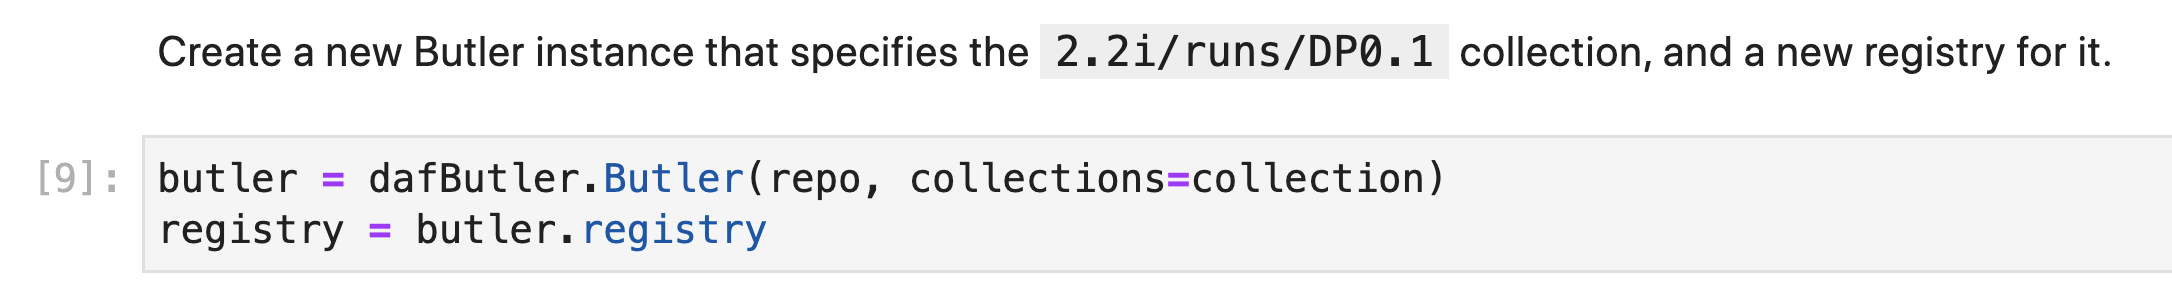
\includegraphics[width=5.46875in]{jira_imgs/2351.png}

}
\begin{tabular}{p{2cm}p{14cm}}
\toprule
Step 2 & Step Execution Status: \textbf{ Pass } \\ \hline
\end{tabular}
 Description \\
{\footnotesize
Call `Butler.get`~

}
\hdashrule[0.5ex]{\textwidth}{1pt}{3mm}
  Expected Result \\
{\footnotesize

}
\hdashrule[0.5ex]{\textwidth}{1pt}{3mm}
  Actual Result \\
{\footnotesize
The notebook reads a calexp image from the butler as
follows:\\[2\baselineskip]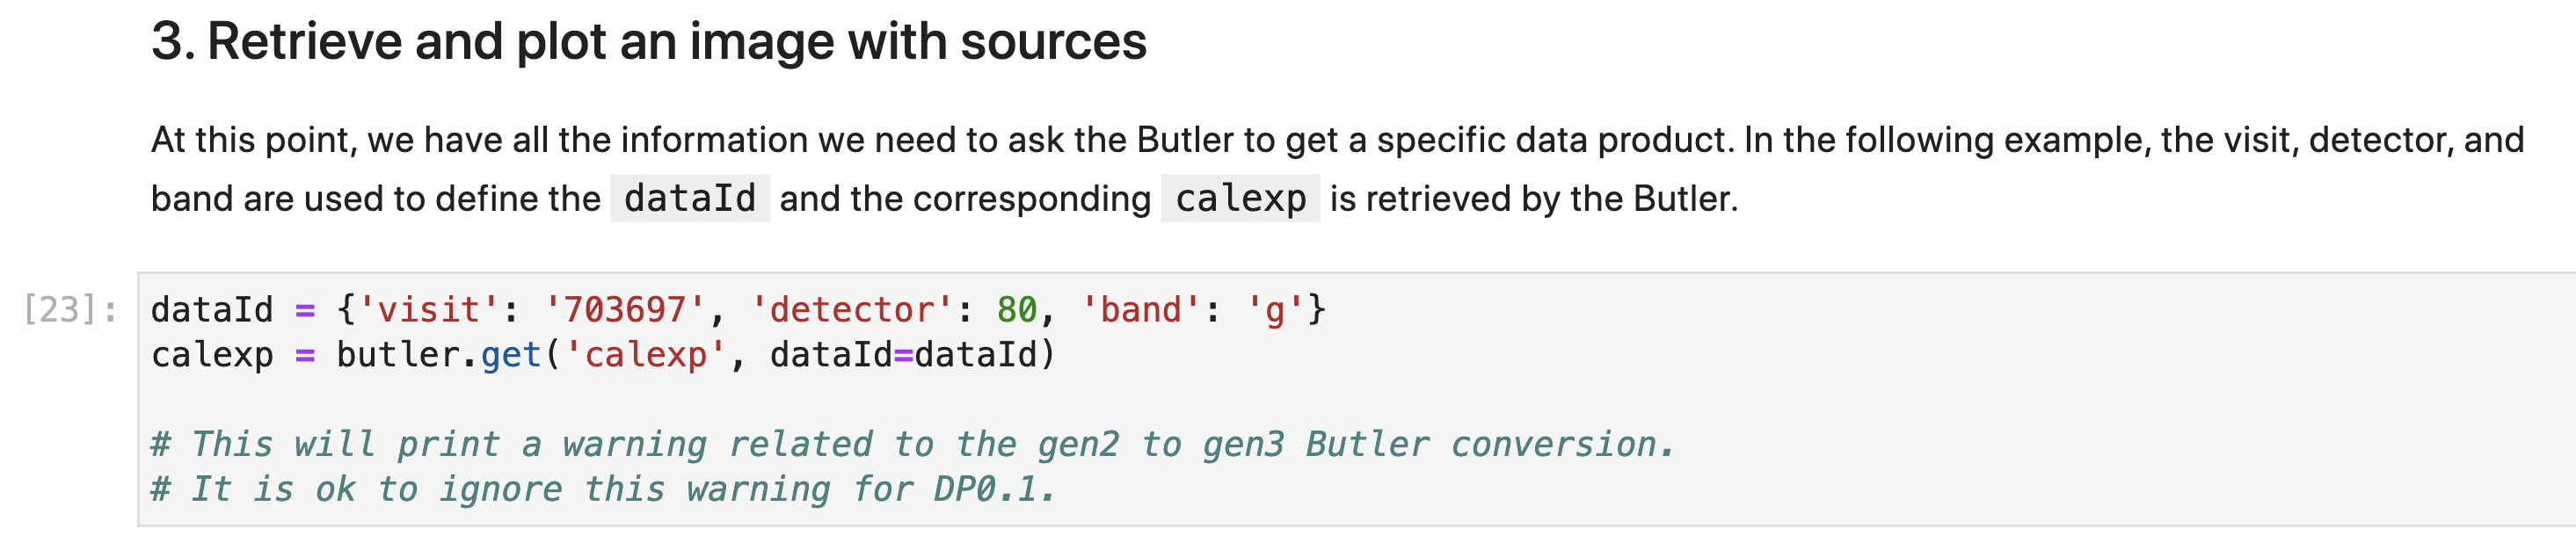
\includegraphics[width=5.92708in]{jira_imgs/2353.png}

}
\begin{tabular}{p{2cm}p{14cm}}
\toprule
Step 3 & Step Execution Status: \textbf{ Pass } \\ \hline
\end{tabular}
 Description \\
{\footnotesize
Verify that data is retrieved

}
\hdashrule[0.5ex]{\textwidth}{1pt}{3mm}
  Expected Result \\
{\footnotesize

}
\hdashrule[0.5ex]{\textwidth}{1pt}{3mm}
  Actual Result \\
{\footnotesize
Confirm that the image has been retrieved by displaying
it:\\[2\baselineskip]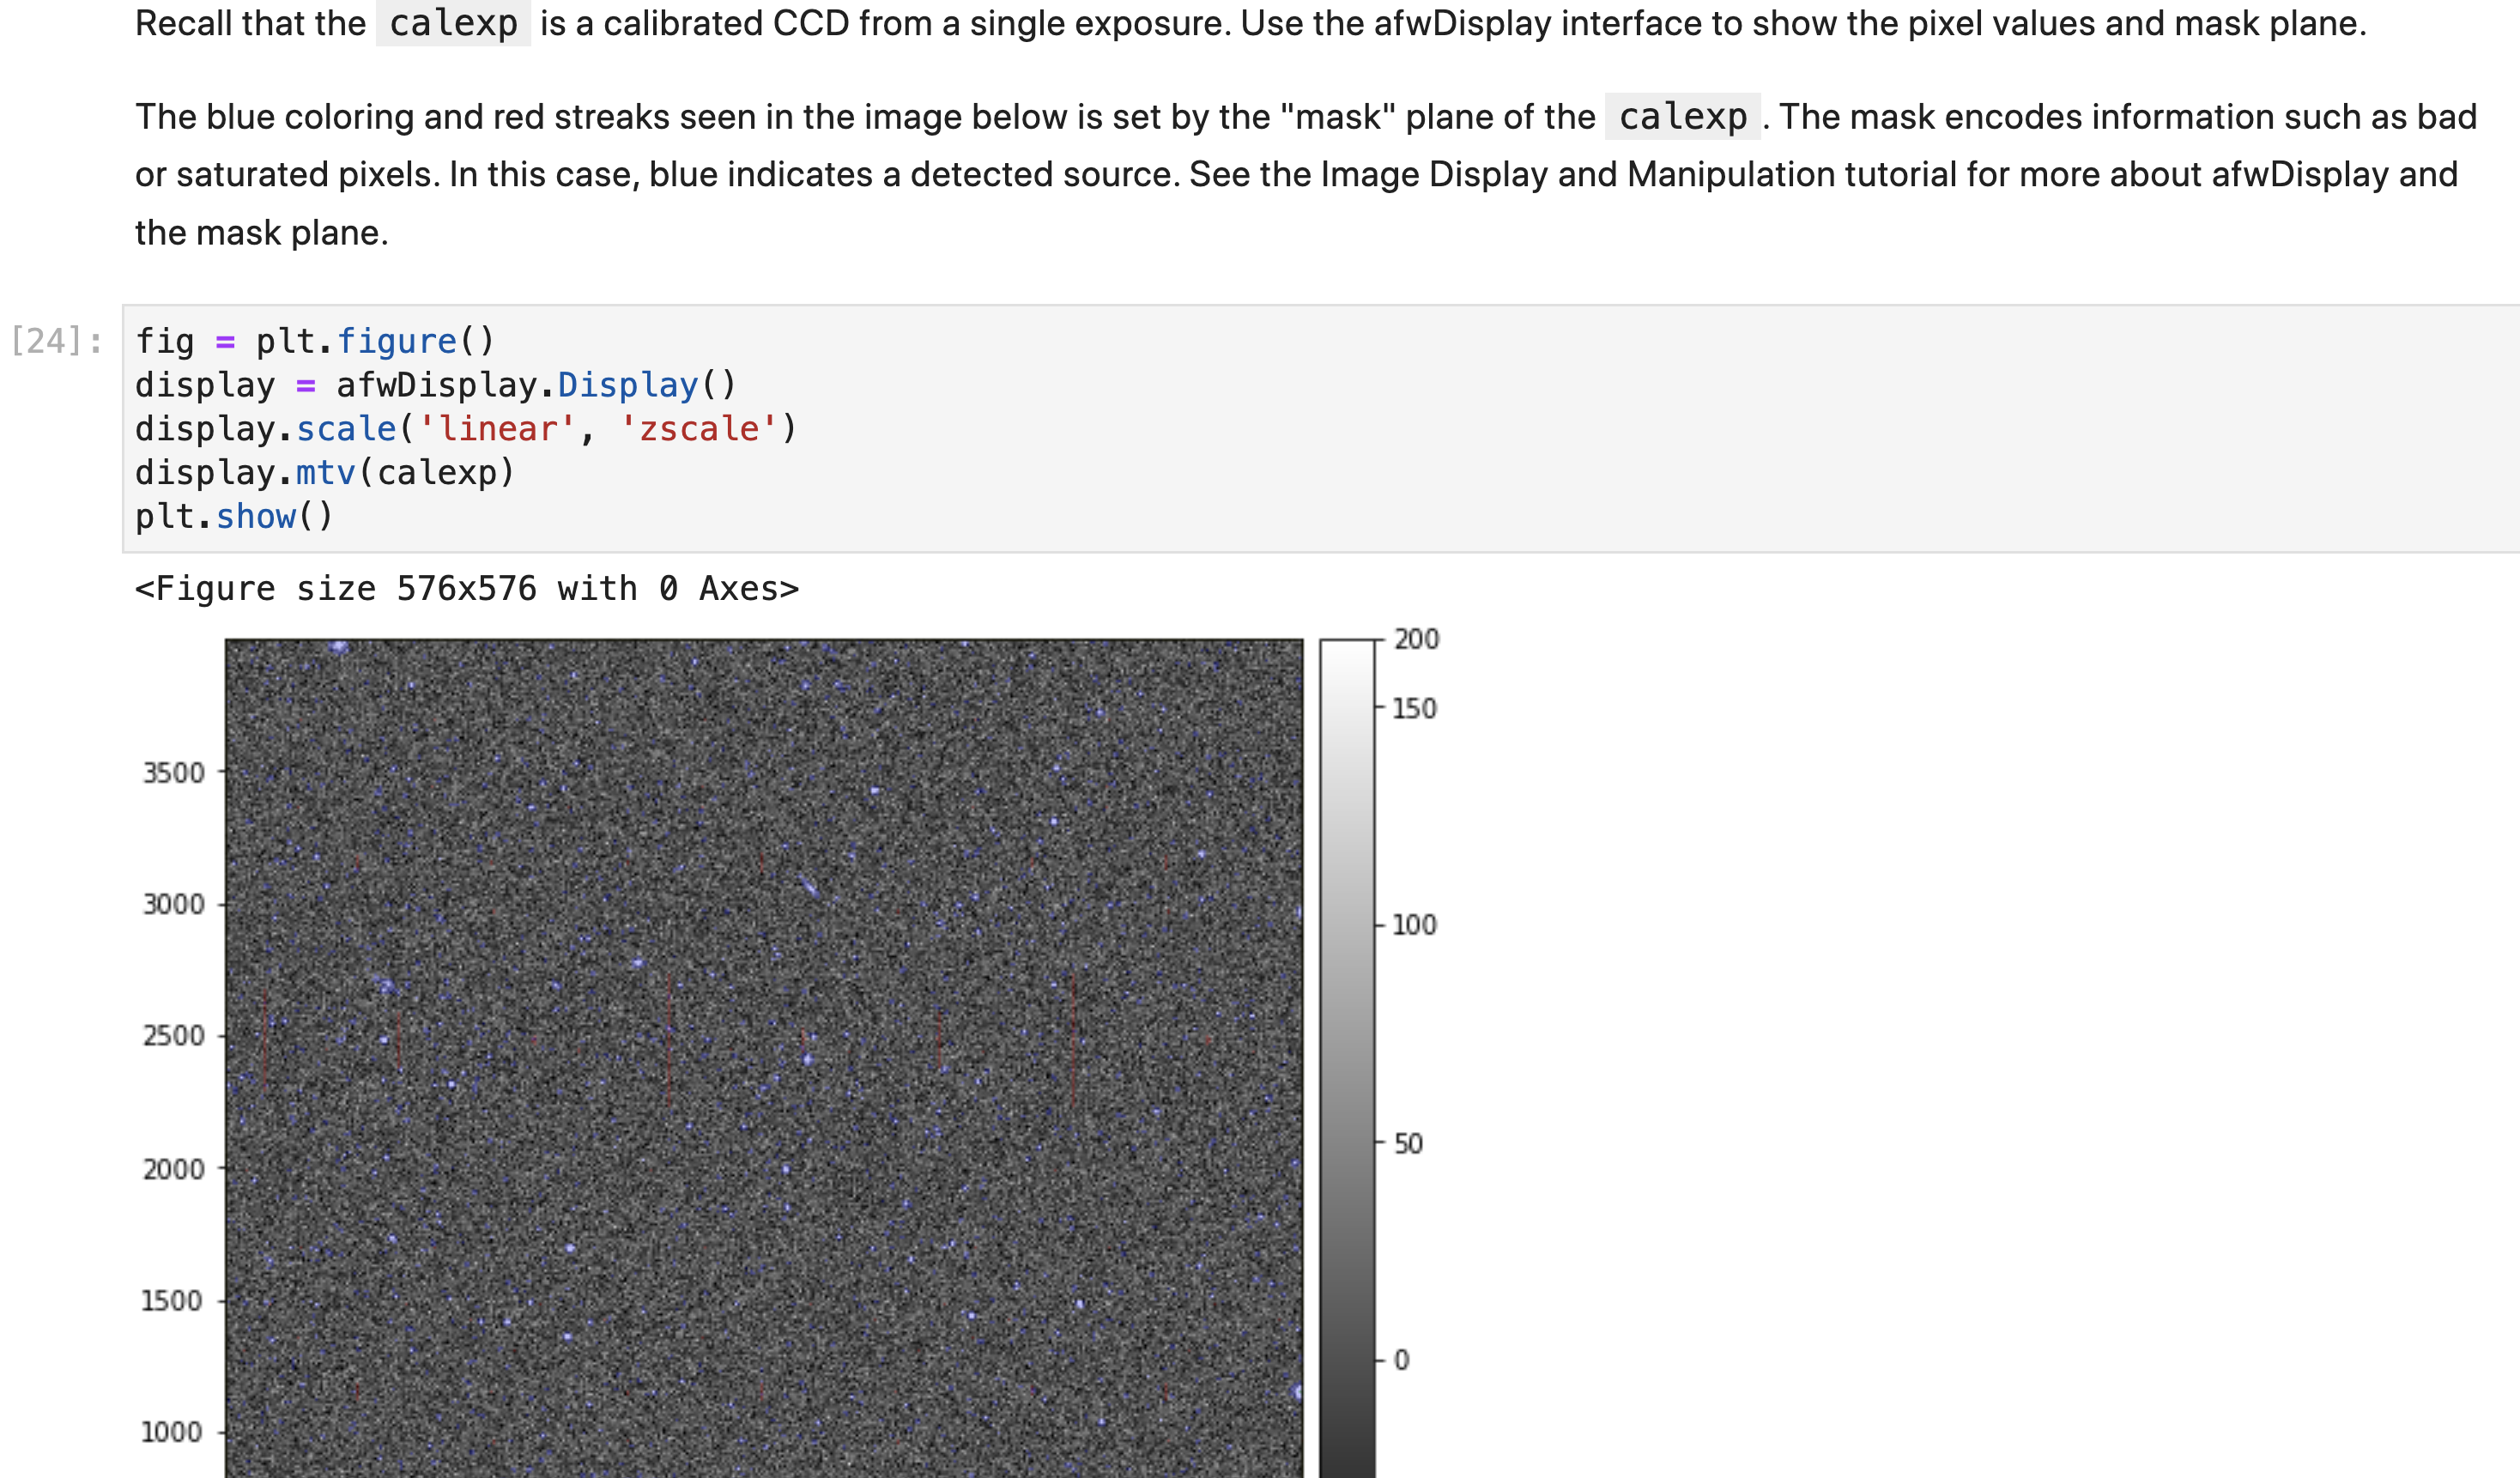
\includegraphics[width=5.20833in]{jira_imgs/2354.png}\\
We have thus demonstrated that data from official Data Releases can be
retrieved from the Science Platform.

}

\paragraph{ LVV-T2486 - Verify Consistent input interface }\mbox{}\\

Version \textbf{1}.
Open  \href{https://jira.lsstcorp.org/secure/Tests.jspa#/testCase/LVV-T2486}{\textit{ LVV-T2486 } }
test case in Jira.

Verify that the Data Input System provides a consistent interface for
loading Datasets into memory given a DatasetRef across different types
of DataRepositories

\textbf{ Preconditions}:\\


Execution status: {\bf Pass }

Final comment:\\


Detailed steps results:

\begin{tabular}{p{2cm}p{14cm}}
\toprule
Step 1 & Step Execution Status: \textbf{ Pass } \\ \hline
\end{tabular}
 Description \\
{\footnotesize
Execute the unit tests at
https://github.com/lsst/daf\_butler/blob/main/tests/test\_butler.py --
in particular, the tests that exercise ImportExport or PutGet in repos
on different types of datastores.

}
\hdashrule[0.5ex]{\textwidth}{1pt}{3mm}
  Expected Result \\
{\footnotesize
Unit tests pass.

}
\hdashrule[0.5ex]{\textwidth}{1pt}{3mm}
  Actual Result \\
{\footnotesize
Working with a cloned `daf\_butler` repository at
/project/jcarlin/SVV/gen3\_middleware\_acceptance\_testing/daf\_butler
on the lsst-devl machines.\\[2\baselineskip]Executed the unit test via:
``pytest -s -vv --no-header
tests/test\_butler.py''\\[2\baselineskip]Among the results, these are
the relevant
tests:\\[2\baselineskip]tests/test\_butler.py::ButlerConfigTests::testSearchPath
PASSED\\
tests/test\_butler.py::PosixDatastoreButlerTestCase::testBasicPutGet
PASSED\\
tests/test\_butler.py::PosixDatastoreButlerTestCase::testButlerRewriteDataId
PASSED\\
tests/test\_butler.py::PosixDatastoreButlerTestCase::testCompositePutGetConcrete
PASSED\\
tests/test\_butler.py::PosixDatastoreButlerTestCase::testCompositePutGetVirtual
PASSED\\
tests/test\_butler.py::PosixDatastoreButlerTestCase::testExportTransferCopy
PASSED\\
tests/test\_butler.py::PosixDatastoreButlerTestCase::testImportExport
Root:
file:///project/jcarlin/SVV/gen3\_middleware\_acceptance\_testing/daf\_butler/tests/tmpfsk\_pyeg/\\
PASSED\\
tests/test\_butler.py::PosixDatastoreButlerTestCase::testIngest PASSED\\
tests/test\_butler.py::PosixDatastoreButlerTestCase::testPutTemplates
PASSED\\[2\baselineskip]tests/test\_butler.py::InMemoryDatastoreButlerTestCase::testBasicPutGet
PASSED\\
tests/test\_butler.py::InMemoryDatastoreButlerTestCase::testButlerRewriteDataId
PASSED\\
tests/test\_butler.py::InMemoryDatastoreButlerTestCase::testCompositePutGetConcrete
PASSED\\
tests/test\_butler.py::InMemoryDatastoreButlerTestCase::testCompositePutGetVirtual
PASSED\\[2\baselineskip]tests/test\_butler.py::ChainedDatastoreButlerTestCase::testBasicPutGet
PASSED\\
tests/test\_butler.py::ChainedDatastoreButlerTestCase::testButlerRewriteDataId
PASSED\\
tests/test\_butler.py::ChainedDatastoreButlerTestCase::testCompositePutGetConcrete
PASSED\\
tests/test\_butler.py::ChainedDatastoreButlerTestCase::testCompositePutGetVirtual
PASSED\\[2\baselineskip]tests/test\_butler.py::ButlerExplicitRootTestCase::testBasicPutGet
PASSED\\
tests/test\_butler.py::ButlerExplicitRootTestCase::testButlerRewriteDataId
PASSED\\
tests/test\_butler.py::ButlerExplicitRootTestCase::testCompositePutGetConcrete
PASSED\\
tests/test\_butler.py::ButlerExplicitRootTestCase::testCompositePutGetVirtual
PASSED\\
tests/test\_butler.py::ButlerExplicitRootTestCase::testExportTransferCopy
PASSED\\
tests/test\_butler.py::ButlerExplicitRootTestCase::testImportExport
Root:
file:///project/jcarlin/SVV/gen3\_middleware\_acceptance\_testing/daf\_butler/tests/tmpvehpotd7/dir1/\\
PASSED\\[2\baselineskip]tests/test\_butler.py::ButlerMakeRepoOutfileTestCase::testConfigExistence
PASSED\\
tests/test\_butler.py::ButlerMakeRepoOutfileTestCase::testDeferredCollectionPassing
PASSED\\
tests/test\_butler.py::ButlerMakeRepoOutfileTestCase::testPutGet
PASSED\\
tests/test\_butler.py::ButlerMakeRepoOutfileDirTestCase::testConfigExistence
PASSED\\
tests/test\_butler.py::ButlerMakeRepoOutfileDirTestCase::testDeferredCollectionPassing
PASSED\\
tests/test\_butler.py::ButlerMakeRepoOutfileDirTestCase::testPutGet
PASSED\\
tests/test\_butler.py::ButlerMakeRepoOutfileUriTestCase::testConfigExistence
PASSED\\
tests/test\_butler.py::ButlerMakeRepoOutfileUriTestCase::testDeferredCollectionPassing
PASSED\\
tests/test\_butler.py::ButlerMakeRepoOutfileUriTestCase::testPutGet
PASSED\\
tests/test\_butler.py::S3DatastoreButlerTestCase::testBasicPutGet
PASSED\\
tests/test\_butler.py::S3DatastoreButlerTestCase::testButlerRewriteDataId
PASSED\\
tests/test\_butler.py::S3DatastoreButlerTestCase::testCompositePutGetConcrete
PASSED\\
tests/test\_butler.py::S3DatastoreButlerTestCase::testCompositePutGetVirtual
PASSED\\
tests/test\_butler.py::S3DatastoreButlerTestCase::testImportExport Root:
s3://anybucketname/CO0O55Y0EX8RB8X9EE5U/\\[2\baselineskip]All of these
unit tests have passed. We have thus demonstrated a consistent interface
for loading Datasets into memory across different types of repositories.

}

\paragraph{ LVV-T2485 - Verify Local caching of remote resources }\mbox{}\\

Version \textbf{1}.
Open  \href{https://jira.lsstcorp.org/secure/Tests.jspa#/testCase/LVV-T2485}{\textit{ LVV-T2485 } }
test case in Jira.

Verify that it is possible to configure the Data Input System to cache a
local version of a Dataset that has been retrieved from a remote
DataRepository.\\[2\baselineskip]Note that this doesn't really look
distinct from DMS-MWBT-REQ-0055 anymore; I think 0055 was perhaps
supposed to be some kind of shared-filesystem proxy for something that
lives on even slower storage, like tape.\\
The specs are similar enough that the same test can be used

\textbf{ Preconditions}:\\


Execution status: {\bf Pass }

Final comment:\\


Detailed steps results:

\begin{tabular}{p{2cm}p{14cm}}
\toprule
Step 1 & Step Execution Status: \textbf{ Pass } \\ \hline
\end{tabular}
 Description \\
{\footnotesize
Enable datastore caching in a Butler client in RSP (or any S3-backed
repo).

}
\hdashrule[0.5ex]{\textwidth}{1pt}{3mm}
  Expected Result \\
{\footnotesize

}
\hdashrule[0.5ex]{\textwidth}{1pt}{3mm}
  Actual Result \\
{\footnotesize
Working at the Interim Data Facility
(at~\href{http://data.lsst.cloud}{data.lsst.cloud}), on which all repos
are S3-backed, and caching is enabled. In a Jupyter notebook, initialize
the butler pointed to an S3 bucket, and switch the cacheManager log
level to
DEBUG:\\[2\baselineskip]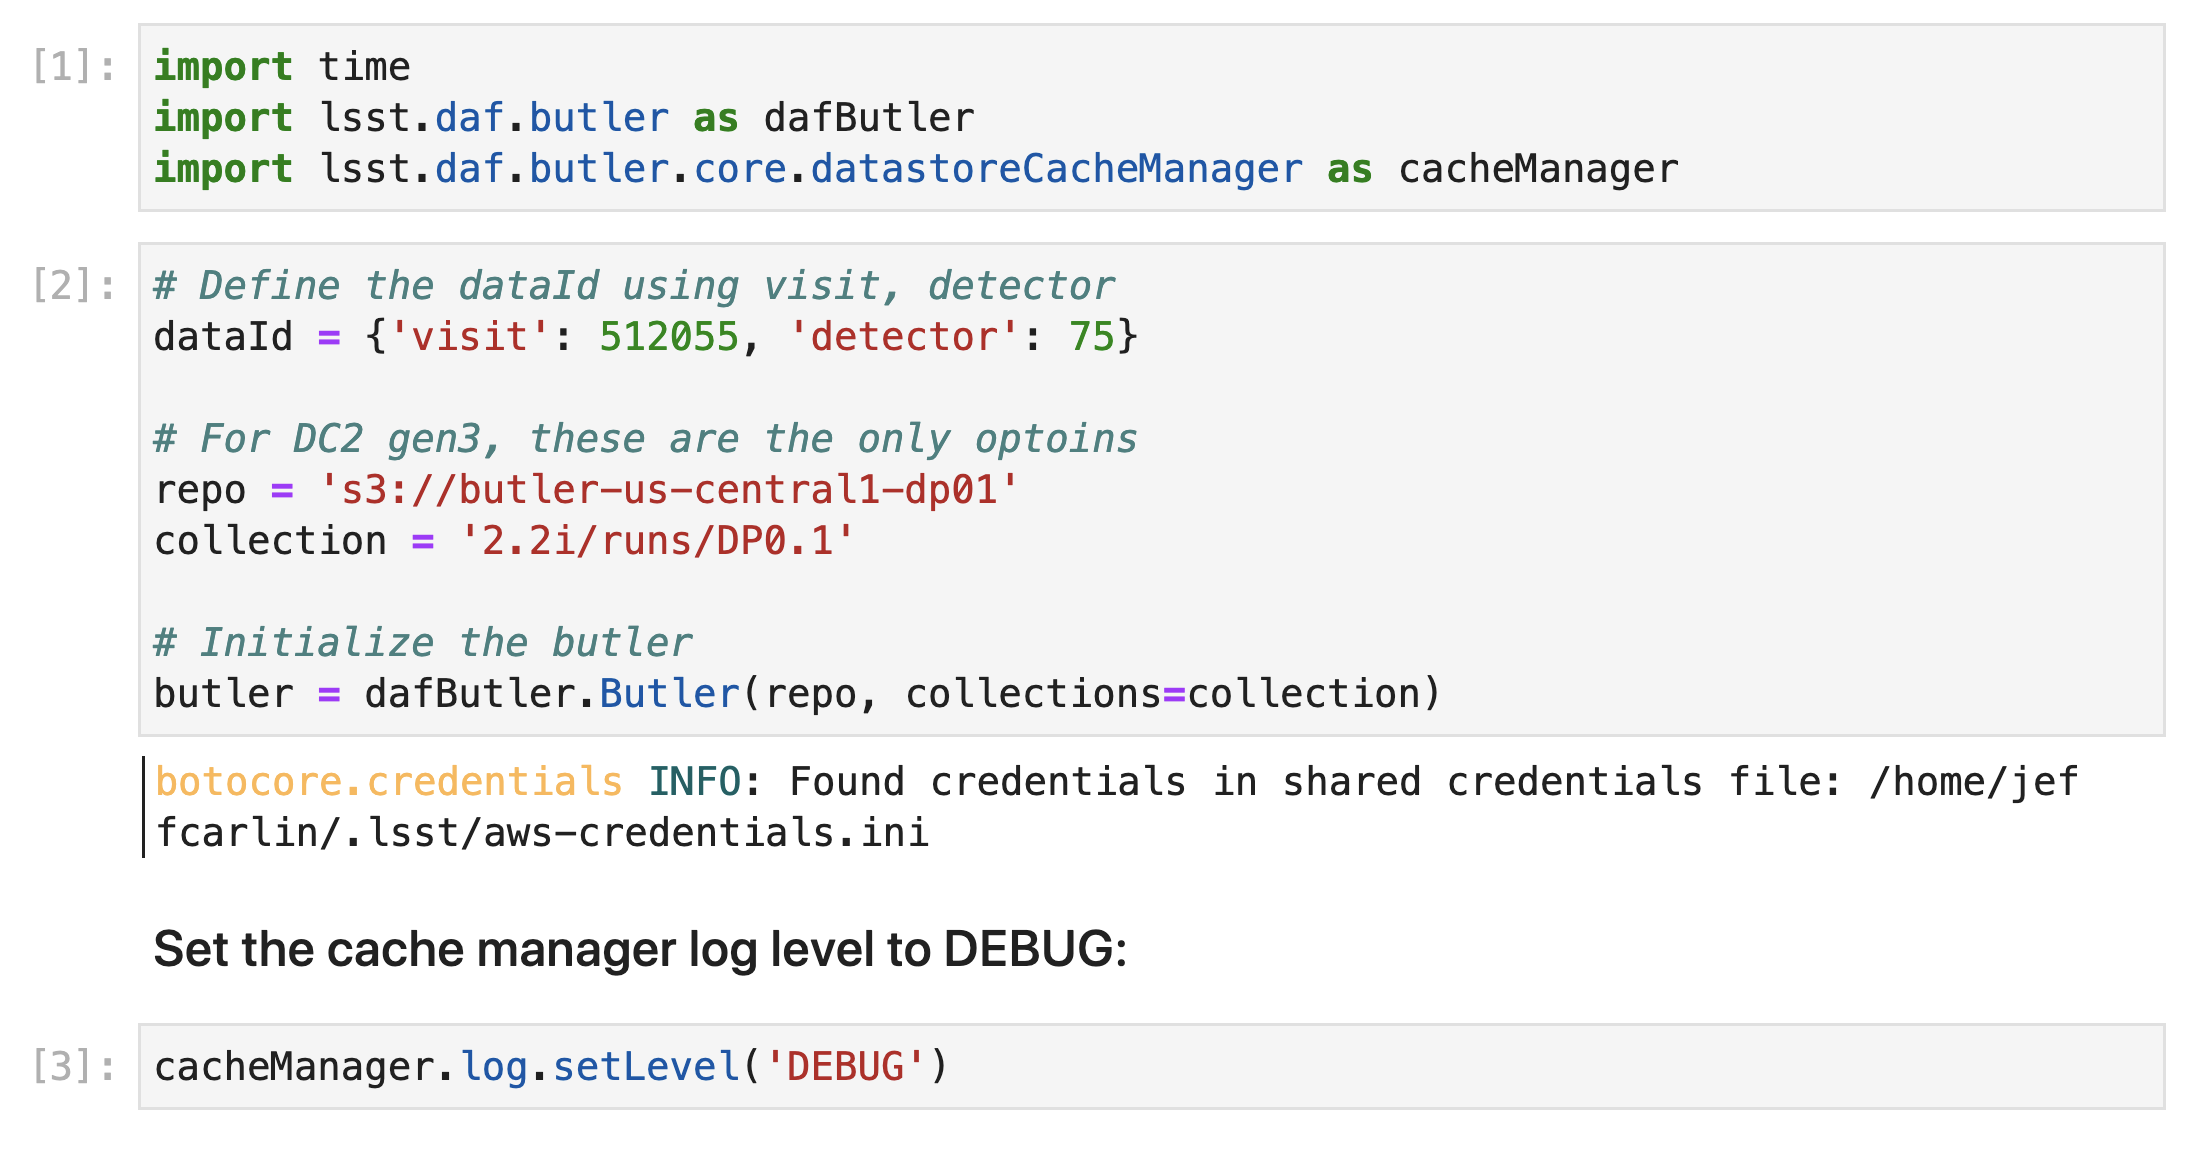
\includegraphics[width=6.68750in]{jira_imgs/2366.png}

}
\begin{tabular}{p{2cm}p{14cm}}
\toprule
Step 2 & Step Execution Status: \textbf{ Pass } \\ \hline
\end{tabular}
 Description \\
{\footnotesize
Run butler.get twice, check (e.g. trace logs) that the second comes from
the cache

}
\hdashrule[0.5ex]{\textwidth}{1pt}{3mm}
  Expected Result \\
{\footnotesize

}
\hdashrule[0.5ex]{\textwidth}{1pt}{3mm}
  Actual Result \\
{\footnotesize
Run butler.get() to extract the `calexp` for the dataId defined in Step
1, inserting timing statements between subsequent calls to demonstrate
speed-up from
caching:\\[2\baselineskip]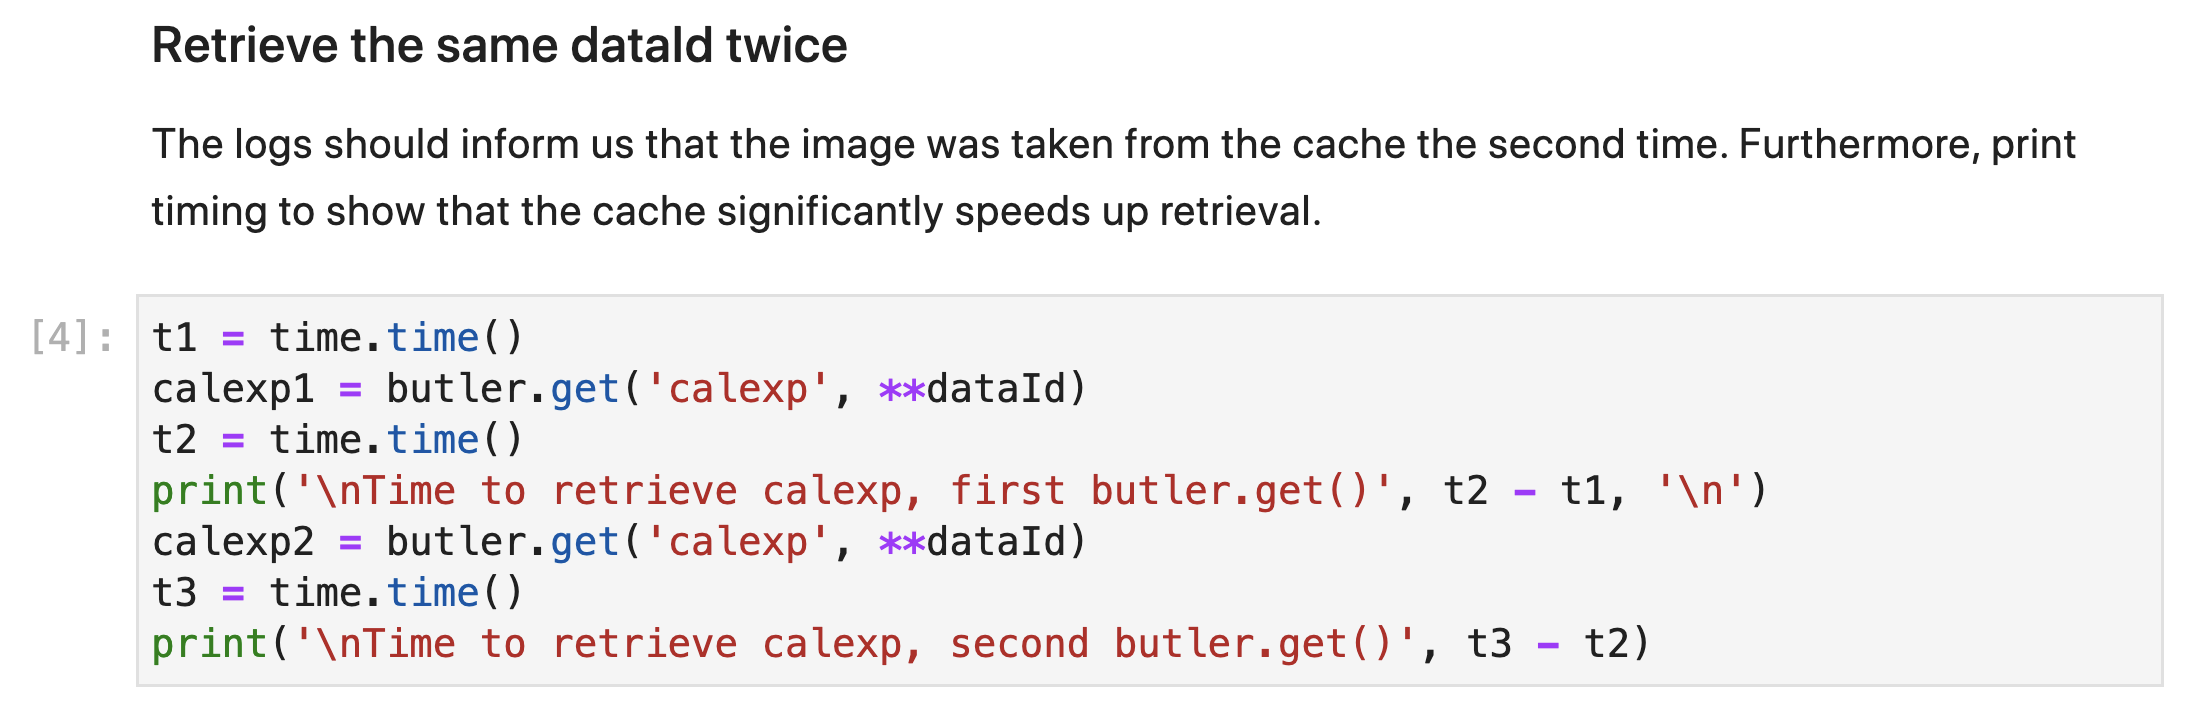
\includegraphics[width=6.19792in]{jira_imgs/2367.png}The
output from this cell is as follows:\\
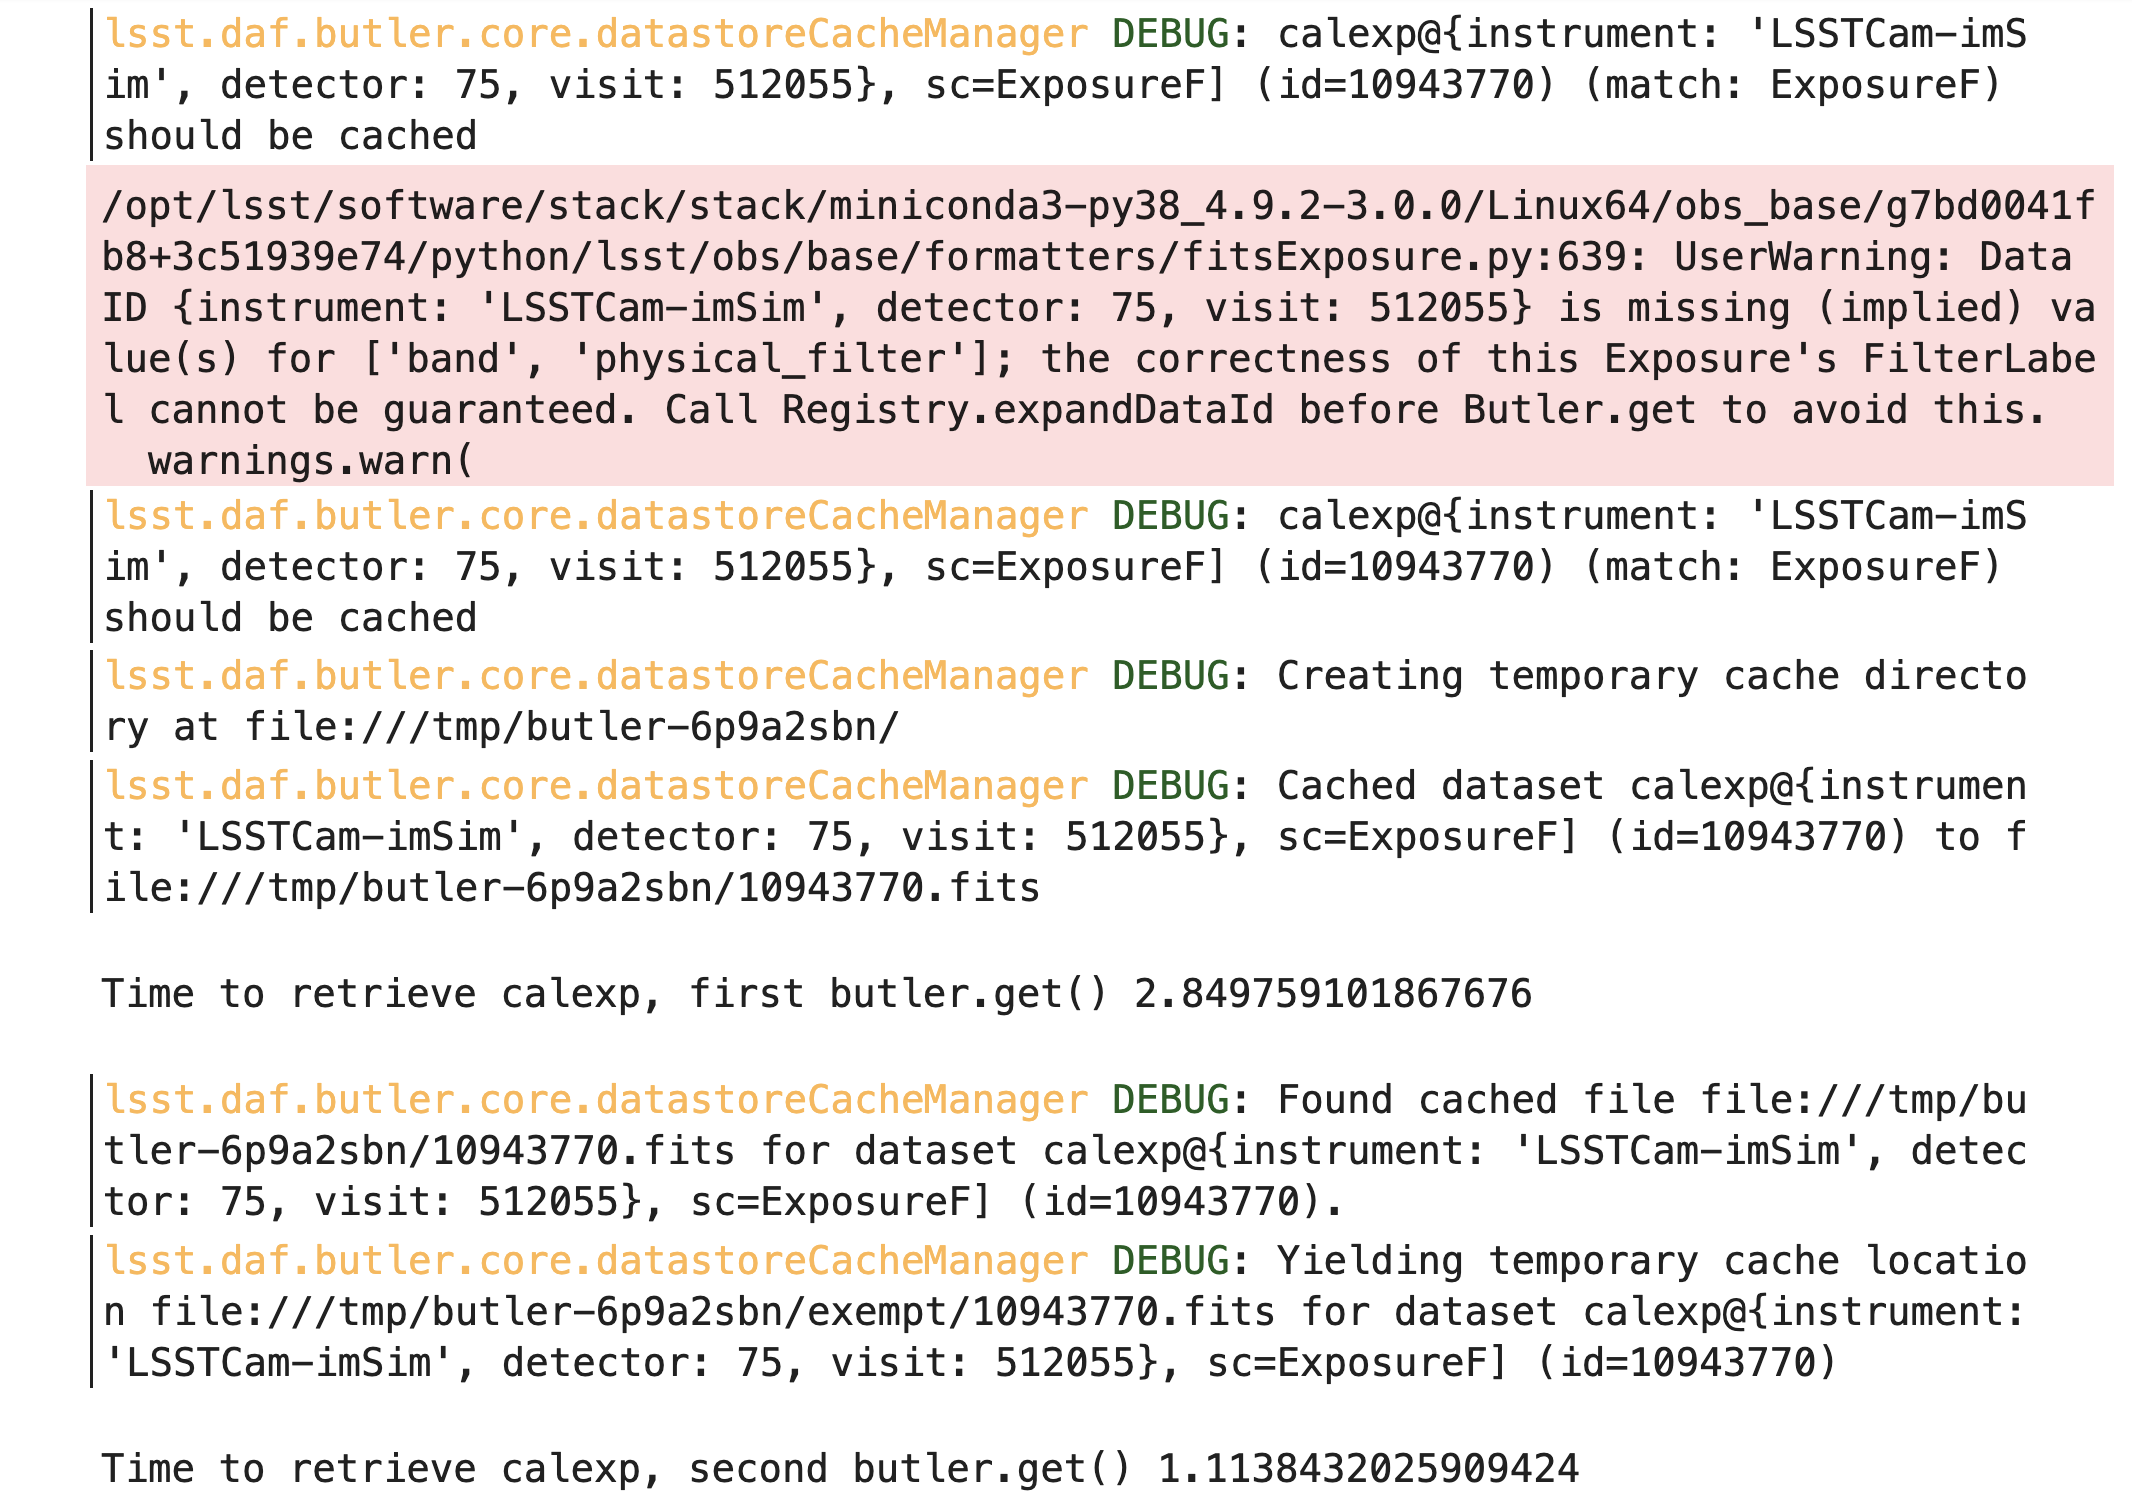
\includegraphics[width=5.67708in]{jira_imgs/2368.png}\\
Note that the timing for the first butler.get() was 2.85 seconds, and
for the second it was 1.11 seconds. The log statements demonstrate that
this is the case because it found the cached file the second time. We
have thus demonstrated local caching of remote resources.

}

\paragraph{ LVV-T2484 - Verify Local proxy }\mbox{}\\

Version \textbf{1}.
Open  \href{https://jira.lsstcorp.org/secure/Tests.jspa#/testCase/LVV-T2484}{\textit{ LVV-T2484 } }
test case in Jira.

Verify that it is possible to configure the Data Input system to use a
local proxy to share remote retrievals of common Datasets

\textbf{ Preconditions}:\\


Execution status: {\bf Not Executed }

Final comment:\\


Detailed steps results:

\begin{tabular}{p{2cm}p{14cm}}
\toprule
Step 1 & Step Execution Status: \textbf{ Not Executed } \\ \hline
\end{tabular}
 Description \\
{\footnotesize
Enable datastore caching in a Butler client in RSP (or any S3-backed
repo).

}
\hdashrule[0.5ex]{\textwidth}{1pt}{3mm}
  Expected Result \\
{\footnotesize

}
\hdashrule[0.5ex]{\textwidth}{1pt}{3mm}
  Actual Result \\
{\footnotesize

}
\begin{tabular}{p{2cm}p{14cm}}
\toprule
Step 2 & Step Execution Status: \textbf{ Not Executed } \\ \hline
\end{tabular}
 Description \\
{\footnotesize
Run `butler.get` twice, check (e.g. trace logs) that the second comes
from the cache.

}
\hdashrule[0.5ex]{\textwidth}{1pt}{3mm}
  Expected Result \\
{\footnotesize

}
\hdashrule[0.5ex]{\textwidth}{1pt}{3mm}
  Actual Result \\
{\footnotesize

}

\paragraph{ LVV-T2483 - Verify Failure on missing input file }\mbox{}\\

Version \textbf{1}.
Open  \href{https://jira.lsstcorp.org/secure/Tests.jspa#/testCase/LVV-T2483}{\textit{ LVV-T2483 } }
test case in Jira.

Verify that it is possible via configuration to require the Data Input
System to fail if an expected file is not found at the specified
location

\textbf{ Preconditions}:\\


Execution status: {\bf Pass }

Final comment:\\


Detailed steps results:

\begin{tabular}{p{2cm}p{14cm}}
\toprule
Step 1 & Step Execution Status: \textbf{ Pass } \\ \hline
\end{tabular}
 Description \\
{\footnotesize
Create a butler repo and ingest some data.

}
\hdashrule[0.5ex]{\textwidth}{1pt}{3mm}
  Expected Result \\
{\footnotesize

}
\hdashrule[0.5ex]{\textwidth}{1pt}{3mm}
  Actual Result \\
{\footnotesize
For this test, we will use the repository we created for
\href{https://jira.lsstcorp.org/secure/Tests.jspa\#/testCase/2873}{LVV-T2478}.
For that test execution, we created an empty Butler repository on the
IDF (called ``repo\_LVV-T2478''), then ingested some raw HSC images into
that repo. Here is a brief snapshot of some contents of that
repo:\\[2\baselineskip]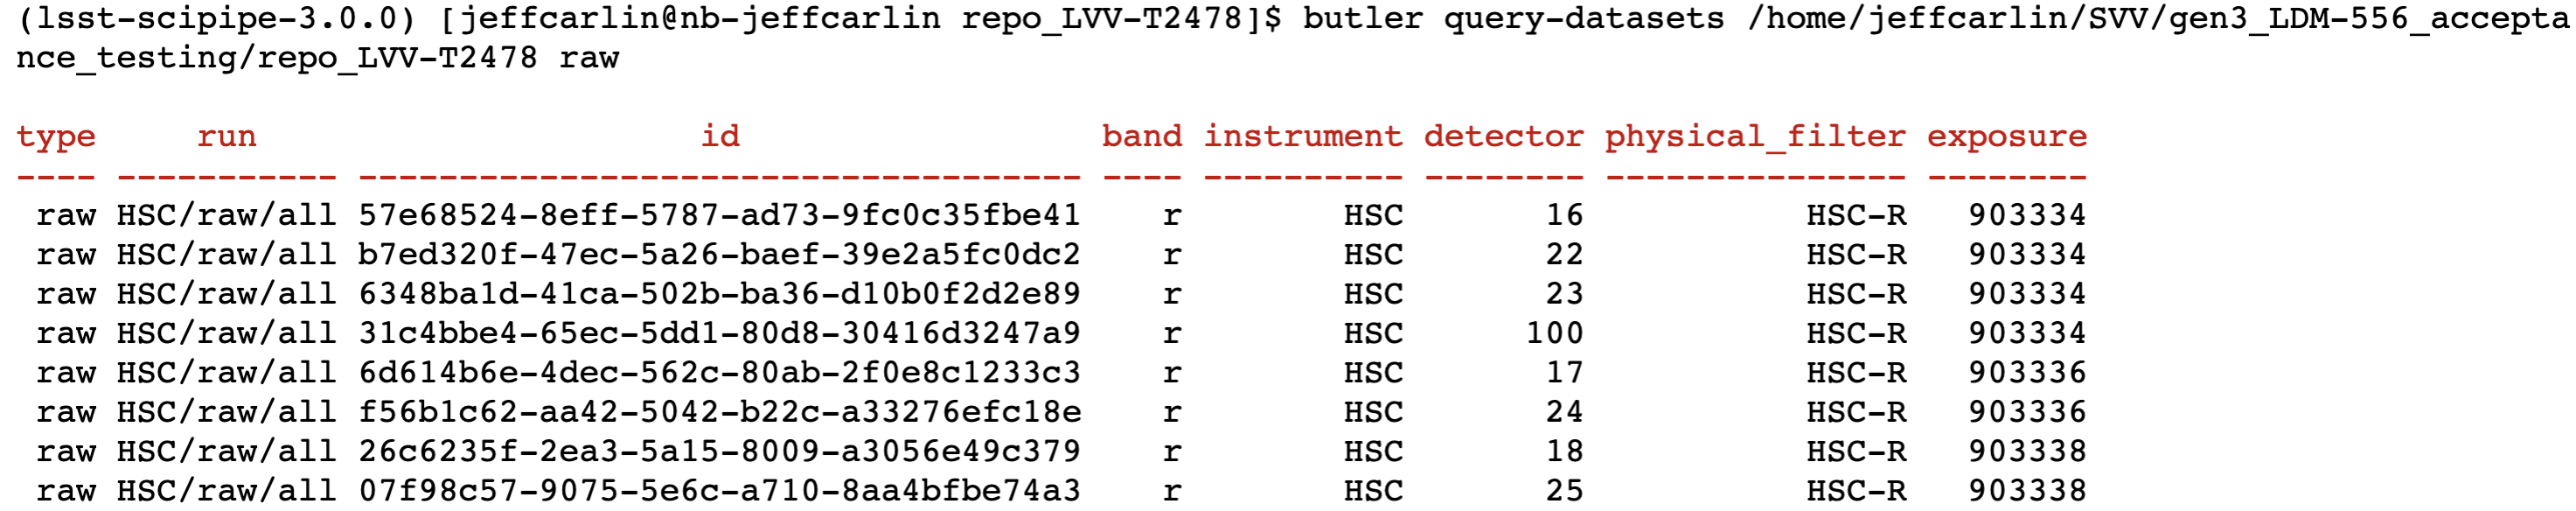
\includegraphics[width=7.58333in]{jira_imgs/2370.png}\\
From the command line, list all of the files in one of the
directories:\\[2\baselineskip](lsst-scipipe-3.0.0)
{[}jeffcarlin@nb-jeffcarlin repo\_LVV-T2478{]}\$ ls
HSC/raw/all/raw/20130617/HSCA90333400/raw\_HSC\_HSC-R\_HSCA90333400\_0\_*.fits\\
HSC/raw/all/raw/20130617/HSCA90333400/raw\_HSC\_HSC-R\_HSCA90333400\_0\_26\_HSC\_raw\_all.fits\\
HSC/raw/all/raw/20130617/HSCA90333400/raw\_HSC\_HSC-R\_HSCA90333400\_0\_27\_HSC\_raw\_all.fits\\
HSC/raw/all/raw/20130617/HSCA90333400/raw\_HSC\_HSC-R\_HSCA90333400\_0\_30\_HSC\_raw\_all.fits\\
HSC/raw/all/raw/20130617/HSCA90333400/raw\_HSC\_HSC-R\_HSCA90333400\_0\_31\_HSC\_raw\_all.fits\\[2\baselineskip]Remove
all of the .fits files from that
directory:\\[2\baselineskip](lsst-scipipe-3.0.0)
{[}jeffcarlin@nb-jeffcarlin repo\_LVV-T2478{]}\$ rm
HSC/raw/all/raw/20130617/HSCA90333400/raw\_HSC\_HSC-R\_HSCA90333400\_0\_*.fits\\
rm: remove regular file
`HSC/raw/all/raw/20130617/HSCA90333400/raw\_HSC\_HSC-R\_HSCA90333400\_0\_26\_HSC\_raw\_all.fits'?
y\\
rm: remove regular file
`HSC/raw/all/raw/20130617/HSCA90333400/raw\_HSC\_HSC-R\_HSCA90333400\_0\_27\_HSC\_raw\_all.fits'?
y\\
rm: remove regular file
`HSC/raw/all/raw/20130617/HSCA90333400/raw\_HSC\_HSC-R\_HSCA90333400\_0\_30\_HSC\_raw\_all.fits'?
y\\
rm: remove regular file
`HSC/raw/all/raw/20130617/HSCA90333400/raw\_HSC\_HSC-R\_HSCA90333400\_0\_31\_HSC\_raw\_all.fits'?
y\\[2\baselineskip]

}
\begin{tabular}{p{2cm}p{14cm}}
\toprule
Step 2 & Step Execution Status: \textbf{ Pass } \\ \hline
\end{tabular}
 Description \\
{\footnotesize
Run `butler.get` against the butler for a datasetRef that does not
exist.

}
\hdashrule[0.5ex]{\textwidth}{1pt}{3mm}
  Expected Result \\
{\footnotesize
Failure (with error message)

}
\hdashrule[0.5ex]{\textwidth}{1pt}{3mm}
  Actual Result \\
{\footnotesize
Open a new notebook, and initialize the butler pointed to this repo.
Provide the dataId for one of the files from Step1. Attempt to retrieve
that file using
butler.get:\\[2\baselineskip]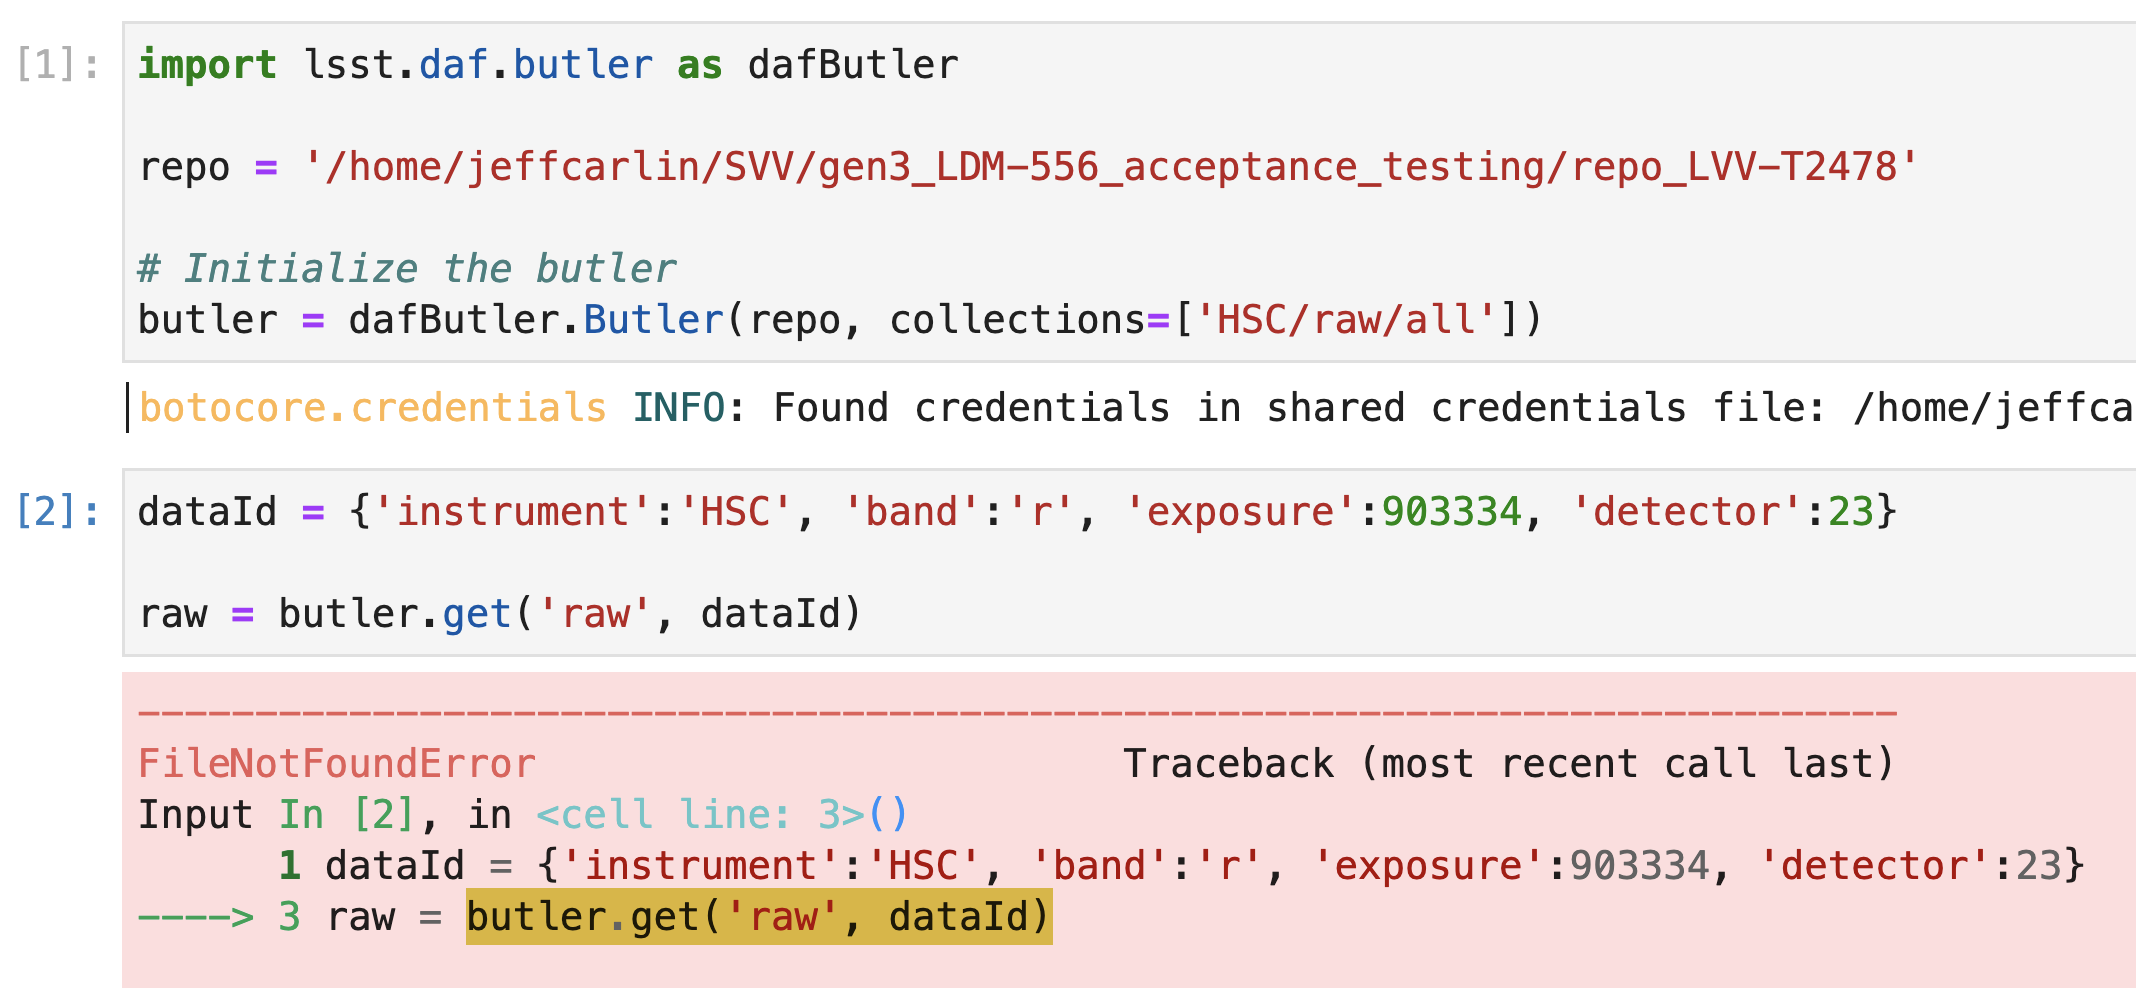
\includegraphics[width=6.81250in]{jira_imgs/2371.png}\\
\ldots{}\\
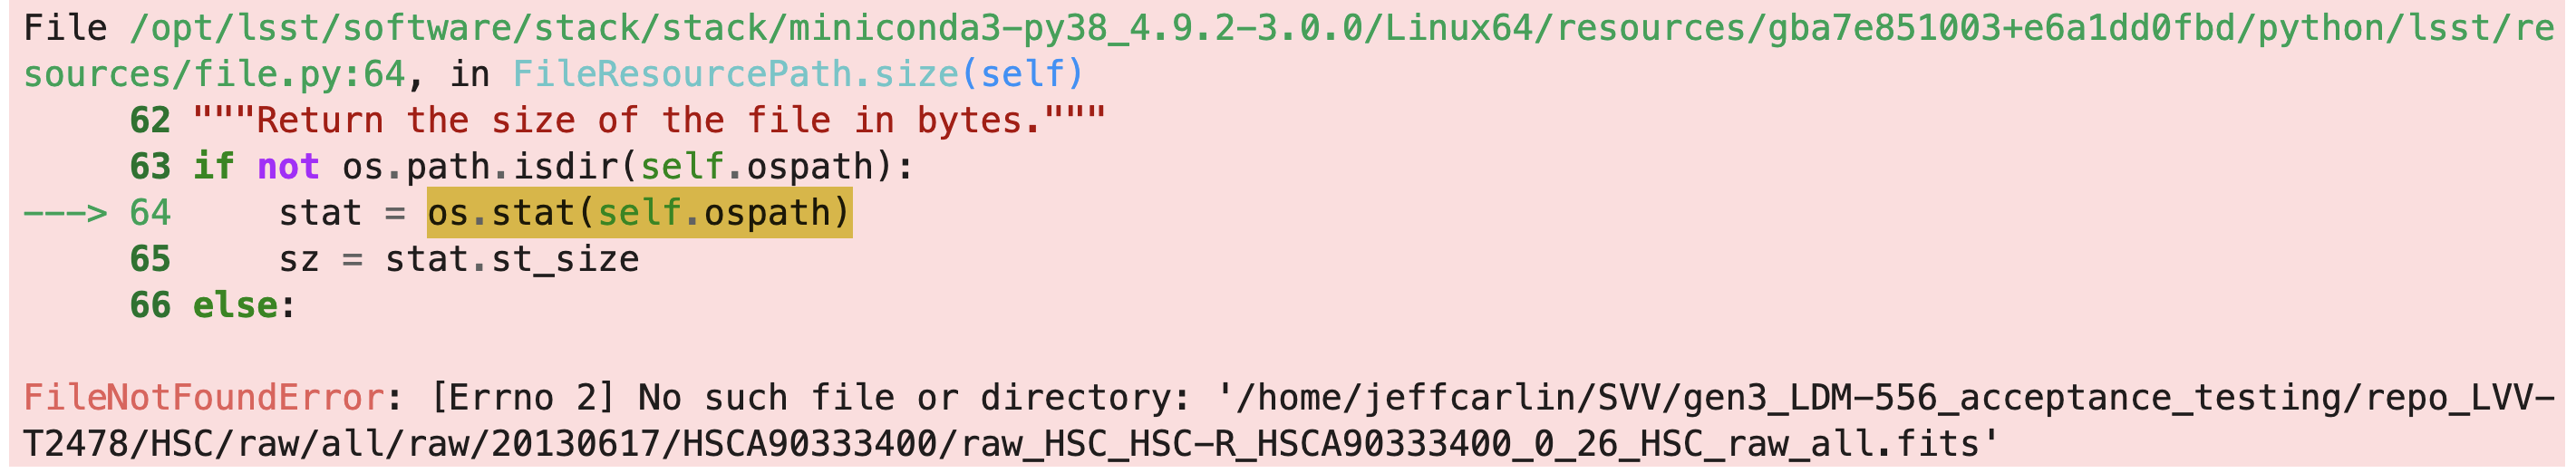
\includegraphics[width=7.63542in]{jira_imgs/2372.png}\\
As expected, we get a FileNotFoundError, thus demonstrating that the
middleware can be required to fail if a requested file is not found at
its expected location.

}

\paragraph{ LVV-T2482 - Verify Enabling PipelineTasks to execute }\mbox{}\\

Version \textbf{1}.
Open  \href{https://jira.lsstcorp.org/secure/Tests.jspa#/testCase/LVV-T2482}{\textit{ LVV-T2482 } }
test case in Jira.

Verify that it is possible for the Data Input System to construct an
InMemoryDataset from a set of files stored locally on disk (without a
remote database connection)

\textbf{ Preconditions}:\\


Execution status: {\bf In Progress }

Final comment:\\


Detailed steps results:

\begin{tabular}{p{2cm}p{14cm}}
\toprule
Step 1 & Step Execution Status: \textbf{ Pass } \\ \hline
\end{tabular}
 Description \\
{\footnotesize
Manually create QG with execution butler

}
\hdashrule[0.5ex]{\textwidth}{1pt}{3mm}
  Expected Result \\
{\footnotesize

}
\hdashrule[0.5ex]{\textwidth}{1pt}{3mm}
  Actual Result \\
{\footnotesize
Create the quantum graph and execution butler for three visits from
tract 9813 in HSC RC2 data located in /repo/main at
NCSA.\\[2\baselineskip]pipetask qgraph -b /repo/main/butler.yaml -p
\$OBS\_SUBARU\_DIR/pipelines/DRP.yaml\#step1\\
\hspace*{0.333em} -i HSC/runs/RC2/w\_2022\_12/DM-34125 -o
u/jcarlin/qgraph\_test\_LDM556 -d ``visit in (1230, 1232, 1240)''\\
-q test.qgraph --save-execution-butler test\_execution\_butler

}
\begin{tabular}{p{2cm}p{14cm}}
\toprule
Step 2 & Step Execution Status: \textbf{ Not Executed } \\ \hline
\end{tabular}
 Description \\
{\footnotesize
Run `butler.get` against execution butler.

}
\hdashrule[0.5ex]{\textwidth}{1pt}{3mm}
  Expected Result \\
{\footnotesize

}
\hdashrule[0.5ex]{\textwidth}{1pt}{3mm}
  Actual Result \\
{\footnotesize
cd test\_execution\_butler/\\[3\baselineskip]

}

\paragraph{ LVV-T2481 - Verify third party datasets }\mbox{}\\

Version \textbf{1}.
Open  \href{https://jira.lsstcorp.org/secure/Tests.jspa#/testCase/LVV-T2481}{\textit{ LVV-T2481 } }
test case in Jira.

Verify that it is possible for the Data Input System to read from
catalogs provided by outside sources using the same interface used for
reading first class LSST datasets via a different plugin.

\textbf{ Preconditions}:\\


Execution status: {\bf Pass }

Final comment:\\


Detailed steps results:

\begin{tabular}{p{2cm}p{14cm}}
\toprule
Step 1 & Step Execution Status: \textbf{ Pass } \\ \hline
\end{tabular}
 Description \\
{\footnotesize
Make an empty repo.\\[2\baselineskip]

}
\hdashrule[0.5ex]{\textwidth}{1pt}{3mm}
  Expected Result \\
{\footnotesize

}
\hdashrule[0.5ex]{\textwidth}{1pt}{3mm}
  Actual Result \\
{\footnotesize
With the science pipelines set up, open an ipython session,
then:\\[2\baselineskip]In {[}1{]}: from lsst.daf.butler import
Butler\\[2\baselineskip]Rather than making an empty repo, we'll create a
new run in an existing butler repository.\\
In {[}2{]}: butler =
Butler(``/project/jcarlin/repos/rc2\_subset/SMALL\_HSC'',
run=``testrun''))

}
\begin{tabular}{p{2cm}p{14cm}}
\toprule
Step 2 & Step Execution Status: \textbf{ Pass } \\ \hline
\end{tabular}
 Description \\
{\footnotesize
Ingest some external parquet or FITS catalog.\\[2\baselineskip]

}
\hdashrule[0.5ex]{\textwidth}{1pt}{3mm}
  Expected Result \\
{\footnotesize

}
\hdashrule[0.5ex]{\textwidth}{1pt}{3mm}
  Actual Result \\
{\footnotesize
In {[}4{]}: from astropy.io import ascii\\[2\baselineskip]Ingest a CSV
catalog that was obtained by searching the WISE catalog via
the~\href{https://irsa.ipac.caltech.edu/frontpage/}{IRSA} archive,
selecting objects within 30 arcsec of MESSIER 033, and saving the
results to a CSV file.\\
In {[}5{]}: tab =
ascii.read(``table\_irsa\_catalog\_search\_results.csv'')\\[2\baselineskip]In
{[}6{]}: tab\\
Out{[}6{]}:\\
\textless{}Table length=8\textgreater{}\\
designation ra dec sigra sigdec sigradec w1mpro w1sigmpro w1snr w1rchi2
\ldots{} w1nm w1m w2nm w2m w3nm w3m w4nm w4m dist angle\\
str19 float64 float64 float64 float64 float64 float64 float64 float64
float64 \ldots{} int64 int64 int64 int64 int64 int64 int64 int64 float64
float64\\
------------------- ---------- ---------- ------- ------- --------
------- --------- ------- ------- \ldots{} ----- ----- ----- ----- -----
----- ----- ----- --------- ----------\\
J013350.89+303936.7 23.462066 30.660195 0.045 0.044 0.0024 10.639 0.025
44.3 14.95 \ldots{} 35 35 35 35 24 24 22 24 0.120773 138.183704\\
J013351.40+303953.2 23.4641735 30.6647787 0.0821 0.086 -0.0237 12.685
0.048 22.4 17.67 \ldots{} 35 35 35 35 24 24 24 24 17.691256 21.927817\\
J013352.24+303942.9 23.4676801 30.6619338 0.0832 0.083 -0.0145 12.574
0.043 25.3 22.31 \ldots{} 35 35 35 35 5 24 19 24 18.523464 70.543114\\
J013351.32+303956.0 23.4638748 30.6655762 0.0842 0.0886 -0.022 12.7
0.051 21.2 16.24 \ldots{} 35 35 35 35 24 24 24 24 20.101993 16.417721\\
J013349.51+303956.4 23.4563181 30.6656714 0.1087 0.1185 -0.0375 13.18
0.125 8.7 2.402 \ldots{} 35 35 35 35 24 24 24 24 26.440434 317.923691\\
J013352.48+303954.9 23.4686874 30.6652703 0.1379 0.1404 -0.0365 13.036
0.059 18.3 11.07 \ldots{} 36 36 35 36 2 24 0 24 27.464228 48.546387\\
J013350.07+303911.3 23.4586394 30.6531485 0.1934 0.2011 -0.054 12.686
0.081 13.5 3.44 \ldots{} 35 35 35 35 0 22 0 24 27.549678 202.47468\\
J013349.03+303951.5 23.4543307 30.6643274 0.1148 0.1222 -0.0355 13.115
0.12 9.1 2.649 \ldots{} 35 35 35 35 24 24 24 24 28.081582
301.775292\\[3\baselineskip]

}
\begin{tabular}{p{2cm}p{14cm}}
\toprule
Step 3 & Step Execution Status: \textbf{ Pass } \\ \hline
\end{tabular}
 Description \\
{\footnotesize
Call butler put~

}
\hdashrule[0.5ex]{\textwidth}{1pt}{3mm}
  Expected Result \\
{\footnotesize

}
\hdashrule[0.5ex]{\textwidth}{1pt}{3mm}
  Actual Result \\
{\footnotesize
Create a dummy dataId:\\
In {[}7{]}: dataId = \{``instrument'': ``WISE'', ``visit'':
423\}\\[2\baselineskip]Register the datasetType:\\
In {[}8{]}: from lsst.daf.butler import DatasetType\\
In {[}9{]}: datasetType = DatasetType(``table'', {[}{]},
``AstropyTable'', universe=butler.registry.dimensions)\\
In {[}10{]}: butler.registry.registerDatasetType(datasetType)\\
Out{[}10{]}: True\\[2\baselineskip]Now use `butler.put` to put the table
into the repo:\\
In {[}11{]}: ref = butler.put(tab,
datasetType)\\[2\baselineskip]Retrieve the table we just put into the
repo:\\
In {[}12{]}: uri = butler.getURI(ref)\\
In {[}13{]}: table = butler.get(``table'')\\[2\baselineskip]Confirm that
we get back the same table we started with:\\
In {[}14{]}: table\\
Out{[}14{]}:\\
\textless{}Table length=8\textgreater{}\\
designation ra dec sigra sigdec sigradec w1mpro w1sigmpro w1snr w1rchi2
\ldots{} w1nm w1m w2nm w2m w3nm w3m w4nm w4m dist angle\\
str19 float64 float64 float64 float64 float64 float64 float64 float64
float64 \ldots{} int64 int64 int64 int64 int64 int64 int64 int64 float64
float64\\
------------------- ---------- ---------- ------- ------- --------
------- --------- ------- ------- \ldots{} ----- ----- ----- ----- -----
----- ----- ----- --------- ----------\\
J013350.89+303936.7 23.462066 30.660195 0.045 0.044 0.0024 10.639 0.025
44.3 14.95 \ldots{} 35 35 35 35 24 24 22 24 0.120773 138.183704\\
J013351.40+303953.2 23.4641735 30.6647787 0.0821 0.086 -0.0237 12.685
0.048 22.4 17.67 \ldots{} 35 35 35 35 24 24 24 24 17.691256 21.927817\\
J013352.24+303942.9 23.4676801 30.6619338 0.0832 0.083 -0.0145 12.574
0.043 25.3 22.31 \ldots{} 35 35 35 35 5 24 19 24 18.523464 70.543114\\
J013351.32+303956.0 23.4638748 30.6655762 0.0842 0.0886 -0.022 12.7
0.051 21.2 16.24 \ldots{} 35 35 35 35 24 24 24 24 20.101993 16.417721\\
J013349.51+303956.4 23.4563181 30.6656714 0.1087 0.1185 -0.0375 13.18
0.125 8.7 2.402 \ldots{} 35 35 35 35 24 24 24 24 26.440434 317.923691\\
J013352.48+303954.9 23.4686874 30.6652703 0.1379 0.1404 -0.0365 13.036
0.059 18.3 11.07 \ldots{} 36 36 35 36 2 24 0 24 27.464228 48.546387\\
J013350.07+303911.3 23.4586394 30.6531485 0.1934 0.2011 -0.054 12.686
0.081 13.5 3.44 \ldots{} 35 35 35 35 0 22 0 24 27.549678 202.47468\\
J013349.03+303951.5 23.4543307 30.6643274 0.1148 0.1222 -0.0355 13.115
0.12 9.1 2.649 \ldots{} 35 35 35 35 24 24 24 24 28.081582 301.775292

}

\paragraph{ LVV-T2480 - Verify Item from Composite Datasets }\mbox{}\\

Version \textbf{1}.
Open  \href{https://jira.lsstcorp.org/secure/Tests.jspa#/testCase/LVV-T2480}{\textit{ LVV-T2480 } }
test case in Jira.

Verify that it is possible ~to load into memory an item from a Composite
Dataset without loading the full Dataset.

\textbf{ Preconditions}:\\


Execution status: {\bf Pass }

Final comment:\\


Detailed steps results:

\begin{tabular}{p{2cm}p{14cm}}
\toprule
Step 1 & Step Execution Status: \textbf{ Pass } \\ \hline
\end{tabular}
 Description \\
{\footnotesize
Use a butler to read a component (e.g. WCS), against any repo.

}
\hdashrule[0.5ex]{\textwidth}{1pt}{3mm}
  Expected Result \\
{\footnotesize

}
\hdashrule[0.5ex]{\textwidth}{1pt}{3mm}
  Actual Result \\
{\footnotesize
On lsst-devl machines at NCSA, with Science Pipelines set
up:\\[2\baselineskip]Open an ipython session:\\[2\baselineskip]\$
ipython\\[2\baselineskip]Import the butler, initialize it for a
collection containing RC2 processing:\\[2\baselineskip]In
{[}\textbf{1}{]}:~\textbf{from} \textbf{lsst.daf.butler} \textbf{import}
Butler\\
In {[}\textbf{2}{]}: butler = Butler(``/repo/main'',
collections={[}``HSC/runs/RC2/w\_2022\_12/DM-34125''{]})\\[2\baselineskip]Select
a random dataId:\\
In {[}\textbf{3}{]}: dataid = \{``visit'': 1230, ``instrument'':
``HSC'', ``detector'': 43\}\\[2\baselineskip]Retrieve the `calexp` and
its associated `wcs`:\\
In {[}\textbf{4}{]}:~calexp = butler.get(``calexp'', dataId=dataid)\\
In {[}\textbf{5}{]}: wcs = butler.get(``calexp.wcs'',
dataId=dataid)\\[2\baselineskip]Examine the `calexp` and `wcs` to
confirm that they are different:\\
In {[}\textbf{6}{]}:~calexp\\
Out{[}\textbf{6}{]}: \textless{}lsst.afw.image.exposure.ExposureF at
0x7f8db02f4f30\textgreater{}\\[2\baselineskip]In {[}\textbf{7}{]}:~wcs\\
Out{[}\textbf{7}{]}:~\\
FITS standard SkyWcs:\\
Sky Origin: (149.8520271457, +2.0585702399)\\
Pixel Origin: (1003.05, 2415.24)\\
Pixel Scale: 0.16713 arcsec/pixel\\[2\baselineskip]They clearly differ
(the `calexp` is an ExposureF type object, while the `wcs` is a FITS
standard SkyWcs). Now confirm that the `wcs` is an item contained within
the composite `calexp` dataset:\\[2\baselineskip]In
{[}\textbf{8}{]}:~calexp.wcs\\
Out{[}\textbf{8}{]}:~\\
FITS standard SkyWcs:\\
Sky Origin: (149.8520271457, +2.0585702399)\\
Pixel Origin: (1003.05, 2415.24)\\
Pixel Scale: 0.16713 arcsec/pixel\\[2\baselineskip]This is identical to
the `wcs` retrieved above, thus demonstrating that the `wcs` item
contained within the composite `calexp` dataset can be retrieved alone,
without loading the entire `calexp`.

}

\paragraph{ LVV-T2479 - Verify Parameterized subset of a Dataset }\mbox{}\\

Version \textbf{1}.
Open  \href{https://jira.lsstcorp.org/secure/Tests.jspa#/testCase/LVV-T2479}{\textit{ LVV-T2479 } }
test case in Jira.

Verify that It is possible to load into memory a parameterized subset of
a Dataset without loading the full Dataset.\\[2\baselineskip]

\textbf{ Preconditions}:\\


Execution status: {\bf Pass }

Final comment:\\


Detailed steps results:

\begin{tabular}{p{2cm}p{14cm}}
\toprule
Step 1 & Step Execution Status: \textbf{ Pass } \\ \hline
\end{tabular}
 Description \\
{\footnotesize
Use a butler to read a subimage via get parameters against any repo.

}
\hdashrule[0.5ex]{\textwidth}{1pt}{3mm}
  Expected Result \\
{\footnotesize

}
\hdashrule[0.5ex]{\textwidth}{1pt}{3mm}
  Actual Result \\
{\footnotesize
On lsst-devl machines at NCSA, with Science Pipelines set
up:\\[2\baselineskip]Open an ipython session:\\[2\baselineskip]\$
ipython\\[2\baselineskip]Import the butler, initialize it for a
collection containing RC2 processing:\\[2\baselineskip]In
{[}\textbf{1}{]}: \textbf{from} \textbf{lsst.daf.butler} \textbf{import}
Butler\\
In {[}\textbf{2}{]}: butler = Butler(``/repo/main'',
collections={[}``HSC/runs/RC2/w\_2022\_12/DM-34125''{]})\\[2\baselineskip]Select
a random dataId:\\
In {[}\textbf{3}{]}: dataid = \{``visit'': 1230, ``instrument'':
``HSC'', ``detector'': 43\}\\[2\baselineskip]Retrieve the `calexp` and
its associated `wcs`:\\
In {[}\textbf{4}{]}:~calexp = butler.get(``calexp'', dataId=dataid)\\
In {[}\textbf{5}{]}: wcs = butler.get(``calexp.wcs'',
dataId=dataid)\\[2\baselineskip]What are the dimensions of this
calexp?\\
In {[}\textbf{32}{]}:~calexp.getDimensions()\\
Out{[}\textbf{32}{]}: Extent2I(2048, 4176)\\[2\baselineskip]Look up the
sky origin of this`calexp`:\\
In {[}\textbf{33}{]}:~wcs.getSkyOrigin()\\
Out{[}\textbf{33}{]}:~SpherePoint(149.85202714570465*degrees,
2.058570239877529*degrees)\\[2\baselineskip]Now, import the ``geom''
package, and create a position slightly shifted from the sky origin on
which to center a cutout image:\\
In {[}\textbf{41}{]}: \textbf{import} \textbf{lsst.geom} \textbf{as}
\textbf{geom}\\
In {[}\textbf{42}{]}: pos = geom.SpherePoint(149.8525, 2.06,
geom.degrees)\\[2\baselineskip]Extract a cutout image with extent of 140
pixels:\\
In {[}\textbf{43}{]}: cutout = butler.get(``calexp'',
dataId=dataid).getCutout(pos,
geom.Extent2I(140))\\[2\baselineskip]Confirm that we have obtained an
image that is smaller than the original `calexp`:\\
In {[}\textbf{44}{]}:~cutout.getDimensions()\\
Out{[}\textbf{44}{]}: Extent2I(140, 140)\\[2\baselineskip]We have thus
demonstrated that a parameterized subset (in this case, a sub-image) of
a Dataset can be loaded into memory without loading the full Dataset.

}

\paragraph{ LVV-T2478 - Verify I/O using cloud storage }\mbox{}\\

Version \textbf{1}.
Open  \href{https://jira.lsstcorp.org/secure/Tests.jspa#/testCase/LVV-T2478}{\textit{ LVV-T2478 } }
test case in Jira.

Verify that the Data Input/Output System shall be able to utilize
cloud-based storage engines.

\textbf{ Preconditions}:\\


Execution status: {\bf Pass }

Final comment:\\


Detailed steps results:

\begin{tabular}{p{2cm}p{14cm}}
\toprule
Step 1 & Step Execution Status: \textbf{ Pass } \\ \hline
\end{tabular}
 Description \\
{\footnotesize
Make an empty repo with an S3 datastore,

}
\hdashrule[0.5ex]{\textwidth}{1pt}{3mm}
  Expected Result \\
{\footnotesize

}
\hdashrule[0.5ex]{\textwidth}{1pt}{3mm}
  Actual Result \\
{\footnotesize
Logged into the Science Platform at the IDF. From the command line in a
terminal, executed the following:\\[2\baselineskip]Set up the LSST
Science Pipelines:\\
(lsst-scipipe-3.0.0) {[}jeffcarlin@nb-jeffcarlin \textasciitilde{}{]}\$
source /opt/lsst/software/stack/loadLSST.bash\\
(lsst-scipipe-3.0.0) {[}jeffcarlin@nb-jeffcarlin \textasciitilde{}{]}\$
setup lsst\_distrib\\[2\baselineskip]Make a directory into which we'll
clone some data:\\
(lsst-scipipe-3.0.0) {[}jeffcarlin@nb-jeffcarlin \textasciitilde{}{]}\$
mkdir repos\\
(lsst-scipipe-3.0.0) {[}jeffcarlin@nb-jeffcarlin \textasciitilde{}{]}\$
cd repos/\\[2\baselineskip]Git clone the test data that is used for
`ci\_hsc`:\\
(lsst-scipipe-3.0.0) {[}jeffcarlin@nb-jeffcarlin \textasciitilde{}{]}\$
git clone
https://github.com/lsst/testdata\_ci\_hsc.git\\[2\baselineskip]Change
directory to the top level, then create a new butler repo:\\
(lsst-scipipe-3.0.0) {[}jeffcarlin@nb-jeffcarlin raw{]}\$ cd\\
(lsst-scipipe-3.0.0) {[}jeffcarlin@nb-jeffcarlin \textasciitilde{}{]}\$
butler create repo\_LVV-T2478\\[2\baselineskip]Register the HSC
instrument with the butler:\\
(lsst-scipipe-3.0.0) {[}jeffcarlin@nb-jeffcarlin \textasciitilde{}{]}\$
butler register-instrument /home/jeffcarlin/repo\_LVV-T2478
lsst.obs.subaru.HyperSuprimeCam\\[2\baselineskip]

}
\begin{tabular}{p{2cm}p{14cm}}
\toprule
Step 2 & Step Execution Status: \textbf{ Pass } \\ \hline
\end{tabular}
 Description \\
{\footnotesize
Run `butler ~get/put`

}
\hdashrule[0.5ex]{\textwidth}{1pt}{3mm}
  Expected Result \\
{\footnotesize

}
\hdashrule[0.5ex]{\textwidth}{1pt}{3mm}
  Actual Result \\
{\footnotesize
Rather than `butler.put`, we will use `ingest-raws` to demonstrate I/O.
Execute `butler ingest-raws`, pointing to the empty repo we just
created, giving it the path to the raw data files we
cloned:\\[2\baselineskip](lsst-scipipe-3.0.0)
{[}jeffcarlin@nb-jeffcarlin \textasciitilde{}{]}\$ butler ingest-raws
/home/jeffcarlin/repo\_LVV-T2478
/home/jeffcarlin/repos/testdata\_ci\_hsc/raw\\
lsst.ingest INFO: Successfully extracted metadata from 33 files with 0
failures\\
lsst.ingest INFO: Exposure HSC:HSCA90398800 ingested successfully\\
lsst.ingest INFO: Exposure HSC:HSCA90334600 ingested successfully\\
lsst.ingest INFO: Exposure HSC:HSCA90334200 ingested successfully\\
lsst.ingest INFO: Exposure HSC:HSCA90333400 ingested successfully\\
lsst.ingest INFO: Exposure HSC:HSCA90333600 ingested successfully\\
lsst.ingest INFO: Exposure HSC:HSCA90399000 ingested successfully\\
lsst.ingest INFO: Exposure HSC:HSCA90401000 ingested successfully\\
lsst.ingest INFO: Exposure HSC:HSCA90333800 ingested successfully\\
lsst.ingest INFO: Exposure HSC:HSCA90398600 ingested successfully\\
lsst.ingest INFO: Exposure HSC:HSCA90401400 ingested successfully\\
lsst.ingest INFO: Exposure HSC:HSCA90334400 ingested successfully\\
lsst.ingest INFO: Successfully processed data from 11 exposures with 0
failures from exposure registration and 0 failures from file ingest.\\
lsst.ingest INFO: Ingested 33 distinct Butler
datasets\\[2\baselineskip]With the successful ingest, we have
demonstrated that the Input/Output system can use cloud storage.

}

\paragraph{ LVV-T2477 - Verify I/O using distributed file system }\mbox{}\\

Version \textbf{1}.
Open  \href{https://jira.lsstcorp.org/secure/Tests.jspa#/testCase/LVV-T2477}{\textit{ LVV-T2477 } }
test case in Jira.

Verify that the Data Input/Output System shall be able to read/write
from/to distributed file systems.

\textbf{ Preconditions}:\\


Execution status: {\bf Pass }

Final comment:\\


Detailed steps results:

\begin{tabular}{p{2cm}p{14cm}}
\toprule
Step 1 & Step Execution Status: \textbf{ Pass } \\ \hline
\end{tabular}
 Description \\
{\footnotesize
Make an empty repo with a POSIX datastore

}
\hdashrule[0.5ex]{\textwidth}{1pt}{3mm}
  Expected Result \\
{\footnotesize

}
\hdashrule[0.5ex]{\textwidth}{1pt}{3mm}
  Actual Result \\
{\footnotesize
Working on the lsst-devl machines at NCSA, in directory
/project/jcarlin/SVV/gen3\_middleware\_acceptance\_testing, with the
LSST Science Pipelines set up.\\[2\baselineskip]Create a new butler
repo:\\
(lsst-scipipe) {[}jcarlin@lsst-devl02
gen3\_middleware\_acceptance\_testing{]}\$ butler create
repo\_LVV-T2477\\[2\baselineskip]Register the HSC instrument with the
butler:\\
(lsst-scipipe) {[}jcarlin@lsst-devl02
gen3\_middleware\_acceptance\_testing{]}\$ butler register-instrument
/project/jcarlin/SVV/gen3\_middleware\_acceptance\_testing/repo\_LVV-T2477
lsst.obs.subaru.HyperSuprimeCam\\[2\baselineskip]

}
\begin{tabular}{p{2cm}p{14cm}}
\toprule
Step 2 & Step Execution Status: \textbf{ Pass } \\ \hline
\end{tabular}
 Description \\
{\footnotesize
~do butler get/put

}
\hdashrule[0.5ex]{\textwidth}{1pt}{3mm}
  Expected Result \\
{\footnotesize

}
\hdashrule[0.5ex]{\textwidth}{1pt}{3mm}
  Actual Result \\
{\footnotesize
Rather than `butler.put`, we will use `ingest-raws` to demonstrate I/O.
Execute `butler ingest-raws`, pointing to the empty repo we just
created, giving it the path to a directory with some raw data
files.\\[2\baselineskip](lsst-scipipe) {[}jcarlin@lsst-devl02
gen3\_middleware\_acceptance\_testing{]}\$ butler ingest-raws
/project/jcarlin/SVV/gen3\_middleware\_acceptance\_testing/repo\_LVV-T2477
/project/jcarlin/repos/testdata\_ci\_hsc/raw\\[2\baselineskip]lsst.ingest
INFO: Successfully extracted metadata from 33 files with 0 failures\\
lsst.ingest INFO: Exposure HSC:HSCA90334600 ingested successfully\\
lsst.ingest INFO: Exposure HSC:HSCA90334400 ingested successfully\\
lsst.ingest INFO: Exposure HSC:HSCA90333800 ingested successfully\\
lsst.ingest INFO: Exposure HSC:HSCA90401000 ingested successfully\\
lsst.ingest INFO: Exposure HSC:HSCA90398600 ingested successfully\\
lsst.ingest INFO: Exposure HSC:HSCA90401400 ingested successfully\\
lsst.ingest INFO: Exposure HSC:HSCA90334200 ingested successfully\\
lsst.ingest INFO: Exposure HSC:HSCA90398800 ingested successfully\\
lsst.ingest INFO: Exposure HSC:HSCA90333600 ingested successfully\\
lsst.ingest INFO: Exposure HSC:HSCA90333400 ingested successfully\\
lsst.ingest INFO: Exposure HSC:HSCA90399000 ingested successfully\\
lsst.ingest INFO: Successfully processed data from 11 exposures with 0
failures from exposure registration and 0 failures from file ingest.\\
lsst.ingest INFO: Ingested 33 distinct Butler
datasets\\[2\baselineskip]With the successful ingest, we have
demonstrated that the Input/Output system can use a distributed file
system.

}

\paragraph{ LVV-T2476 - Verify Format Plugability }\mbox{}\\

Version \textbf{1}.
Open  \href{https://jira.lsstcorp.org/secure/Tests.jspa#/testCase/LVV-T2476}{\textit{ LVV-T2476 } }
test case in Jira.

Verify that it is possible to control the method used to read and write
a particular DatasetType using a text configuration file such that the
Python object and the form of the persisted dataset can be configured
externally.

\textbf{ Preconditions}:\\


Execution status: {\bf Not Executed }

Final comment:\\


Detailed steps results:

\begin{tabular}{p{2cm}p{14cm}}
\toprule
Step 1 & Step Execution Status: \textbf{ Not Executed } \\ \hline
\end{tabular}
 Description \\
{\footnotesize
Make an empty repo with the default configuration.

}
\hdashrule[0.5ex]{\textwidth}{1pt}{3mm}
  Expected Result \\
{\footnotesize

}
\hdashrule[0.5ex]{\textwidth}{1pt}{3mm}
  Actual Result \\
{\footnotesize

}
\begin{tabular}{p{2cm}p{14cm}}
\toprule
Step 2 & Step Execution Status: \textbf{ Not Executed } \\ \hline
\end{tabular}
 Description \\
{\footnotesize
Make an empty repo with configuration that overrides a
formatter.\\[2\baselineskip]

}
\hdashrule[0.5ex]{\textwidth}{1pt}{3mm}
  Expected Result \\
{\footnotesize

}
\hdashrule[0.5ex]{\textwidth}{1pt}{3mm}
  Actual Result \\
{\footnotesize

}
\begin{tabular}{p{2cm}p{14cm}}
\toprule
Step 3 & Step Execution Status: \textbf{ Not Executed } \\ \hline
\end{tabular}
 Description \\
{\footnotesize
Make an empty repo with configuration that changes a StorageClass's
Python

}
\hdashrule[0.5ex]{\textwidth}{1pt}{3mm}
  Expected Result \\
{\footnotesize

}
\hdashrule[0.5ex]{\textwidth}{1pt}{3mm}
  Actual Result \\
{\footnotesize

}
\begin{tabular}{p{2cm}p{14cm}}
\toprule
Step 4 & Step Execution Status: \textbf{ Not Executed } \\ \hline
\end{tabular}
 Description \\
{\footnotesize
Put and get the same datasets to all repos.

}
\hdashrule[0.5ex]{\textwidth}{1pt}{3mm}
  Expected Result \\
{\footnotesize

}
\hdashrule[0.5ex]{\textwidth}{1pt}{3mm}
  Actual Result \\
{\footnotesize

}

\paragraph{ LVV-T2474 - Verify Data Discovery for Data Release Production }\mbox{}\\

Version \textbf{1}.
Open  \href{https://jira.lsstcorp.org/secure/Tests.jspa#/testCase/LVV-T2474}{\textit{ LVV-T2474 } }
test case in Jira.

Verify that the Data Discovery System interface is usable when
initiating processing for Data Release Production.

\textbf{ Preconditions}:\\


Execution status: {\bf Pass }

Final comment:\\


Detailed steps results:

\begin{tabular}{p{2cm}p{14cm}}
\toprule
Step 1 & Step Execution Status: \textbf{ Pass } \\ \hline
\end{tabular}
 Description \\
{\footnotesize
Run QG generation for the DRP pipeline against any major repo (e.g.
`/repo/main`). ~Same as
for~\href{https://jira.lsstcorp.org/secure/Tests.jspa\#/testCase/LVV-T2473}{LVV-T2473}

}
\hdashrule[0.5ex]{\textwidth}{1pt}{3mm}
  Expected Result \\
{\footnotesize

}
\hdashrule[0.5ex]{\textwidth}{1pt}{3mm}
  Actual Result \\
{\footnotesize
At NCSA, on lsst-devl machines, with science pipelines set
up.\\[2\baselineskip]Generate a quantum graph by executing ``step1'' of
the standard DRP pipeline against a recent reprocessing of HSC RC2
data:\\[2\baselineskip]pipetask qgraph -b /repo/main/butler.yaml -p
\$OBS\_SUBARU\_DIR/pipelines/DRP.yaml\#step1 -i
HSC/runs/RC2/w\_2022\_12/DM-34125 -o
u/jcarlin/qgraph\_test\_LDM556\_step1 -d ``visit in (1230, 1232) AND
detector in (42, 43)'' -q rc2\_step1.qgraph\\[2\baselineskip]This
prepares the quantum graph illustrating ``step1'' processing of two
visits and two detectors from the RC2 dataset, and saves the graph as
``rc2\_step1.qgraph''.\\[2\baselineskip]To illustrate that the graph is
well-formed, examine the ``graph'' output by executing:\\
pipetask qgraph -b /repo/main/butler.yaml -g rc2\_step1.qgraph --show
graph\\[2\baselineskip]Outputs:\\
TaskDef(lsst.ip.isr.isrTask.IsrTask, label=isr)\\
Quantum 0:\\
inputs:\\
DatasetType('raw', \{band, instrument, detector, physical\_filter,
exposure\}, Exposure): {[}DataId(\{instrument: `HSC', detector: 43,
exposure: 1230, \ldots{}\}){]}\\
DatasetType('linearizer', \{instrument, detector\}, Linearizer,
isCalibration=True): {[}{]}\\
DatasetType('isrOverscanCorrected', \{band, instrument, detector,
physical\_filter, exposure\}, Exposure): {[}{]}\\
DatasetType('bias', \{instrument, detector\}, ExposureF,
isCalibration=True): {[}DataId(\{instrument: `HSC', detector: 43\}){]}\\
DatasetType('transmission\_filter', \{band, instrument,
physical\_filter\}, TransmissionCurve, isCalibration=True):
{[}DataId(\{instrument: `HSC', physical\_filter: `HSC-I',
\ldots{}\}){]}\\
DatasetType('bfKernel', \{instrument\}, NumpyArray, isCalibration=True):
{[}DataId(\{instrument: `HSC'\}){]}\\
DatasetType('transmission\_optics', \{instrument\}, TransmissionCurve,
isCalibration=True): {[}DataId(\{instrument: `HSC'\}){]}\\
DatasetType('crosstalk', \{instrument, detector\}, CrosstalkCalib,
isCalibration=True): {[}{]}\\
DatasetType('fringe', \{band, instrument, detector, physical\_filter\},
ExposureF, isCalibration=True): {[}{]}\\
DatasetType('transmission\_sensor', \{instrument, detector\},
TransmissionCurve, isCalibration=True): {[}DataId(\{instrument: `HSC',
detector: 43\}){]}\\
DatasetType('flat', \{band, instrument, detector, physical\_filter\},
ExposureF, isCalibration=True): {[}DataId(\{instrument: `HSC', detector:
43, physical\_filter: `HSC-I', \ldots{}\}){]}\\
DatasetType('camera', \{instrument\}, Camera, isCalibration=True):
{[}DataId(\{instrument: `HSC'\}){]}\\
DatasetType('transmission\_atmosphere', \{instrument\},
TransmissionCurve, isCalibration=True): {[}DataId(\{instrument:
`HSC'\}){]}\\
DatasetType('dark', \{instrument, detector\}, ExposureF,
isCalibration=True): {[}DataId(\{instrument: `HSC', detector: 43\}){]}\\
DatasetType('yBackground', \{band, instrument, detector,
physical\_filter\}, StrayLightData, isCalibration=True): {[}{]}\\
DatasetType('defects', \{instrument, detector\}, Defects,
isCalibration=True): {[}DataId(\{instrument: `HSC', detector: 43\}){]}\\
DatasetType('brighterFatterKernel', \{instrument, detector\},
BrighterFatterKernel, isCalibration=True): {[}{]}\\
outputs:\\
DatasetType('postISRCCD', \{band, instrument, detector,
physical\_filter, exposure\}, Exposure): {[}DataId(\{instrument: `HSC',
detector: 43, exposure: 1230, \ldots{}\}){]}\\
DatasetType('isr\_metadata', \{band, instrument, detector,
physical\_filter, exposure\}, PropertySet): {[}DataId(\{instrument:
`HSC', detector: 43, exposure: 1230, \ldots{}\}){]}\\
DatasetType('isr\_log', \{band, instrument, detector, physical\_filter,
exposure\}, ButlerLogRecords): {[}DataId(\{instrument: `HSC', detector:
43, exposure: 1230, \ldots{}\}){]}\\
Quantum 1:\\
inputs:\\
DatasetType('raw', \{band, instrument, detector, physical\_filter,
exposure\}, Exposure): {[}DataId(\{instrument: `HSC', detector: 43,
exposure: 1232, \ldots{}\}){]}\\
DatasetType('linearizer', \{instrument, detector\}, Linearizer,
isCalibration=True):
{[}{]}\\[2\baselineskip]\ldots{}\\[2\baselineskip]TaskDef(lsst.pipe.tasks.postprocess.WriteSourceTableTask,
label=writeSourceTable)\\
Quantum 0:\\
inputs:\\
DatasetType('src', \{band, instrument, detector, physical\_filter,
visit\_system, visit\}, SourceCatalog): {[}DataId(\{instrument: `HSC',
detector: 43, visit: 1232, \ldots{}\}){]}\\
outputs:\\
DatasetType('writeSourceTable\_metadata', \{band, instrument, detector,
physical\_filter, visit\_system, visit\}, PropertySet):
{[}DataId(\{instrument: `HSC', detector: 43, visit: 1232,
\ldots{}\}){]}\\
DatasetType('source', \{band, instrument, detector, physical\_filter,
visit\_system, visit\}, DataFrame): {[}DataId(\{instrument: `HSC',
detector: 43, visit: 1232, \ldots{}\}){]}\\
DatasetType('writeSourceTable\_log', \{band, instrument, detector,
physical\_filter, visit\_system, visit\}, ButlerLogRecords):
{[}DataId(\{instrument: `HSC', detector: 43, visit: 1232,
\ldots{}\}){]}\\
Quantum 1:\\
inputs:\\
DatasetType('src', \{band, instrument, detector, physical\_filter,
visit\_system, visit\}, SourceCatalog): {[}DataId(\{instrument: `HSC',
detector: 42, visit: 1230, \ldots{}\}){]}\\
outputs:\\
DatasetType('writeSourceTable\_metadata', \{band, instrument, detector,
physical\_filter, visit\_system, visit\}, PropertySet):
{[}DataId(\{instrument: `HSC', detector: 42, visit: 1230,
\ldots{}\}){]}\\
DatasetType('source', \{band, instrument, detector, physical\_filter,
visit\_system, visit\}, DataFrame): {[}DataId(\{instrument: `HSC',
detector: 42, visit: 1230, \ldots{}\}){]}\\
DatasetType('writeSourceTable\_log', \{band, instrument, detector,
physical\_filter, visit\_system, visit\}, ButlerLogRecords):
{[}DataId(\{instrument: `HSC', detector: 42, visit: 1230,
\ldots{}\}){]}\\
Quantum 2:\\
inputs:\\
DatasetType('src', \{band, instrument, detector, physical\_filter,
visit\_system, visit\}, SourceCatalog): {[}DataId(\{instrument: `HSC',
detector: 42, visit: 1232, \ldots{}\}){]}\\
outputs:\\
DatasetType('writeSourceTable\_metadata', \{band, instrument, detector,
physical\_filter, visit\_system, visit\}, PropertySet):
{[}DataId(\{instrument: `HSC', detector: 42, visit: 1232,
\ldots{}\}){]}\\
DatasetType('source', \{band, instrument, detector, physical\_filter,
visit\_system, visit\}, DataFrame): {[}DataId(\{instrument: `HSC',
detector: 42, visit: 1232, \ldots{}\}){]}\\
DatasetType('writeSourceTable\_log', \{band, instrument, detector,
physical\_filter, visit\_system, visit\}, ButlerLogRecords):
{[}DataId(\{instrument: `HSC', detector: 42, visit: 1232,
\ldots{}\}){]}\\
Quantum 3:\\
inputs:\\
DatasetType('src', \{band, instrument, detector, physical\_filter,
visit\_system, visit\}, SourceCatalog): {[}DataId(\{instrument: `HSC',
detector: 43, visit: 1230, \ldots{}\}){]}\\
outputs:\\
DatasetType('writeSourceTable\_metadata', \{band, instrument, detector,
physical\_filter, visit\_system, visit\}, PropertySet):
{[}DataId(\{instrument: `HSC', detector: 43, visit: 1230,
\ldots{}\}){]}\\
DatasetType('source', \{band, instrument, detector, physical\_filter,
visit\_system, visit\}, DataFrame): {[}DataId(\{instrument: `HSC',
detector: 43, visit: 1230, \ldots{}\}){]}\\
DatasetType('writeSourceTable\_log', \{band, instrument, detector,
physical\_filter, visit\_system, visit\}, ButlerLogRecords):
{[}DataId(\{instrument: `HSC', detector: 43, visit: 1230,
\ldots{}\}){]}\\[2\baselineskip](truncated for display) This shows the
quanta and the tasks to be executed for each. This graph file
demonstrates that the Data Discovery System can be used to initiate Data
Release Production runs.

}

\paragraph{ LVV-T2475 - Verify Data discovery for test processing runs }\mbox{}\\

Version \textbf{1}.
Open  \href{https://jira.lsstcorp.org/secure/Tests.jspa#/testCase/LVV-T2475}{\textit{ LVV-T2475 } }
test case in Jira.

Verify that the ~Data Discovery System interface is~ usable when
initiating processing runs initiated for test/development purposes (on
LSST or personal hardware),

\textbf{ Preconditions}:\\


Execution status: {\bf Pass }

Final comment:\\


Detailed steps results:

\begin{tabular}{p{2cm}p{14cm}}
\toprule
Step 1 & Step Execution Status: \textbf{ Pass } \\ \hline
\end{tabular}
 Description \\
{\footnotesize
Run QG generation for the DRP pipeline against any major repo (e.g.
`/repo/main`). ~Same as for
\href{https://jira.lsstcorp.org/secure/Tests.jspa\#/testCase/LVV-T2473}{LVV-T2473}

}
\hdashrule[0.5ex]{\textwidth}{1pt}{3mm}
  Expected Result \\
{\footnotesize

}
\hdashrule[0.5ex]{\textwidth}{1pt}{3mm}
  Actual Result \\
{\footnotesize
At NCSA, on lsst-devl machines, with science pipelines set
up.\\[2\baselineskip]Generate a quantum graph by executing ``step1'' of
the standard DRP pipeline against a recent reprocessing of HSC RC2
data:\\[2\baselineskip]pipetask qgraph -b /repo/main/butler.yaml -p
\$OBS\_SUBARU\_DIR/pipelines/DRP.yaml\#step1 -i
HSC/runs/RC2/w\_2022\_12/DM-34125 -o
u/jcarlin/qgraph\_test\_LDM556\_step1 -d ``visit in (1230, 1232) AND
detector in (42, 43)'' -q rc2\_step1.qgraph\\[2\baselineskip]This
prepares the quantum graph illustrating ``step1'' processing of two
visits and two detectors from the RC2 dataset, and saves the graph as
``rc2\_step1.qgraph''.\\[2\baselineskip]To illustrate that the graph is
well-formed, examine the ``graph'' output by executing:\\
pipetask qgraph -b /repo/main/butler.yaml -g rc2\_step1.qgraph --show
graph\\[2\baselineskip]Outputs:\\
TaskDef(lsst.ip.isr.isrTask.IsrTask, label=isr)\\
Quantum 0:\\
inputs:\\
DatasetType('raw', \{band, instrument, detector, physical\_filter,
exposure\}, Exposure): {[}DataId(\{instrument: `HSC', detector: 43,
exposure: 1230, \ldots{}\}){]}\\
DatasetType('linearizer', \{instrument, detector\}, Linearizer,
isCalibration=True): {[}{]}\\
DatasetType('isrOverscanCorrected', \{band, instrument, detector,
physical\_filter, exposure\}, Exposure): {[}{]}\\
DatasetType('bias', \{instrument, detector\}, ExposureF,
isCalibration=True): {[}DataId(\{instrument: `HSC', detector: 43\}){]}\\
DatasetType('transmission\_filter', \{band, instrument,
physical\_filter\}, TransmissionCurve, isCalibration=True):
{[}DataId(\{instrument: `HSC', physical\_filter: `HSC-I',
\ldots{}\}){]}\\
DatasetType('bfKernel', \{instrument\}, NumpyArray, isCalibration=True):
{[}DataId(\{instrument: `HSC'\}){]}\\
DatasetType('transmission\_optics', \{instrument\}, TransmissionCurve,
isCalibration=True): {[}DataId(\{instrument: `HSC'\}){]}\\
DatasetType('crosstalk', \{instrument, detector\}, CrosstalkCalib,
isCalibration=True): {[}{]}\\
DatasetType('fringe', \{band, instrument, detector, physical\_filter\},
ExposureF, isCalibration=True): {[}{]}\\
DatasetType('transmission\_sensor', \{instrument, detector\},
TransmissionCurve, isCalibration=True): {[}DataId(\{instrument: `HSC',
detector: 43\}){]}\\
DatasetType('flat', \{band, instrument, detector, physical\_filter\},
ExposureF, isCalibration=True): {[}DataId(\{instrument: `HSC', detector:
43, physical\_filter: `HSC-I', \ldots{}\}){]}\\
DatasetType('camera', \{instrument\}, Camera, isCalibration=True):
{[}DataId(\{instrument: `HSC'\}){]}\\
DatasetType('transmission\_atmosphere', \{instrument\},
TransmissionCurve, isCalibration=True): {[}DataId(\{instrument:
`HSC'\}){]}\\
DatasetType('dark', \{instrument, detector\}, ExposureF,
isCalibration=True): {[}DataId(\{instrument: `HSC', detector: 43\}){]}\\
DatasetType('yBackground', \{band, instrument, detector,
physical\_filter\}, StrayLightData, isCalibration=True): {[}{]}\\
DatasetType('defects', \{instrument, detector\}, Defects,
isCalibration=True): {[}DataId(\{instrument: `HSC', detector: 43\}){]}\\
DatasetType('brighterFatterKernel', \{instrument, detector\},
BrighterFatterKernel, isCalibration=True): {[}{]}\\
outputs:\\
DatasetType('postISRCCD', \{band, instrument, detector,
physical\_filter, exposure\}, Exposure): {[}DataId(\{instrument: `HSC',
detector: 43, exposure: 1230, \ldots{}\}){]}\\
DatasetType('isr\_metadata', \{band, instrument, detector,
physical\_filter, exposure\}, PropertySet): {[}DataId(\{instrument:
`HSC', detector: 43, exposure: 1230, \ldots{}\}){]}\\
DatasetType('isr\_log', \{band, instrument, detector, physical\_filter,
exposure\}, ButlerLogRecords): {[}DataId(\{instrument: `HSC', detector:
43, exposure: 1230, \ldots{}\}){]}\\
Quantum 1:\\
inputs:\\
DatasetType('raw', \{band, instrument, detector, physical\_filter,
exposure\}, Exposure): {[}DataId(\{instrument: `HSC', detector: 43,
exposure: 1232, \ldots{}\}){]}\\
DatasetType('linearizer', \{instrument, detector\}, Linearizer,
isCalibration=True):
{[}{]}\\[2\baselineskip]\ldots{}\\[2\baselineskip]TaskDef(lsst.pipe.tasks.postprocess.WriteSourceTableTask,
label=writeSourceTable)\\
Quantum 0:\\
inputs:\\
DatasetType('src', \{band, instrument, detector, physical\_filter,
visit\_system, visit\}, SourceCatalog): {[}DataId(\{instrument: `HSC',
detector: 43, visit: 1232, \ldots{}\}){]}\\
outputs:\\
DatasetType('writeSourceTable\_metadata', \{band, instrument, detector,
physical\_filter, visit\_system, visit\}, PropertySet):
{[}DataId(\{instrument: `HSC', detector: 43, visit: 1232,
\ldots{}\}){]}\\
DatasetType('source', \{band, instrument, detector, physical\_filter,
visit\_system, visit\}, DataFrame): {[}DataId(\{instrument: `HSC',
detector: 43, visit: 1232, \ldots{}\}){]}\\
DatasetType('writeSourceTable\_log', \{band, instrument, detector,
physical\_filter, visit\_system, visit\}, ButlerLogRecords):
{[}DataId(\{instrument: `HSC', detector: 43, visit: 1232,
\ldots{}\}){]}\\
Quantum 1:\\
inputs:\\
DatasetType('src', \{band, instrument, detector, physical\_filter,
visit\_system, visit\}, SourceCatalog): {[}DataId(\{instrument: `HSC',
detector: 42, visit: 1230, \ldots{}\}){]}\\
outputs:\\
DatasetType('writeSourceTable\_metadata', \{band, instrument, detector,
physical\_filter, visit\_system, visit\}, PropertySet):
{[}DataId(\{instrument: `HSC', detector: 42, visit: 1230,
\ldots{}\}){]}\\
DatasetType('source', \{band, instrument, detector, physical\_filter,
visit\_system, visit\}, DataFrame): {[}DataId(\{instrument: `HSC',
detector: 42, visit: 1230, \ldots{}\}){]}\\
DatasetType('writeSourceTable\_log', \{band, instrument, detector,
physical\_filter, visit\_system, visit\}, ButlerLogRecords):
{[}DataId(\{instrument: `HSC', detector: 42, visit: 1230,
\ldots{}\}){]}\\
Quantum 2:\\
inputs:\\
DatasetType('src', \{band, instrument, detector, physical\_filter,
visit\_system, visit\}, SourceCatalog): {[}DataId(\{instrument: `HSC',
detector: 42, visit: 1232, \ldots{}\}){]}\\
outputs:\\
DatasetType('writeSourceTable\_metadata', \{band, instrument, detector,
physical\_filter, visit\_system, visit\}, PropertySet):
{[}DataId(\{instrument: `HSC', detector: 42, visit: 1232,
\ldots{}\}){]}\\
DatasetType('source', \{band, instrument, detector, physical\_filter,
visit\_system, visit\}, DataFrame): {[}DataId(\{instrument: `HSC',
detector: 42, visit: 1232, \ldots{}\}){]}\\
DatasetType('writeSourceTable\_log', \{band, instrument, detector,
physical\_filter, visit\_system, visit\}, ButlerLogRecords):
{[}DataId(\{instrument: `HSC', detector: 42, visit: 1232,
\ldots{}\}){]}\\
Quantum 3:\\
inputs:\\
DatasetType('src', \{band, instrument, detector, physical\_filter,
visit\_system, visit\}, SourceCatalog): {[}DataId(\{instrument: `HSC',
detector: 43, visit: 1230, \ldots{}\}){]}\\
outputs:\\
DatasetType('writeSourceTable\_metadata', \{band, instrument, detector,
physical\_filter, visit\_system, visit\}, PropertySet):
{[}DataId(\{instrument: `HSC', detector: 43, visit: 1230,
\ldots{}\}){]}\\
DatasetType('source', \{band, instrument, detector, physical\_filter,
visit\_system, visit\}, DataFrame): {[}DataId(\{instrument: `HSC',
detector: 43, visit: 1230, \ldots{}\}){]}\\
DatasetType('writeSourceTable\_log', \{band, instrument, detector,
physical\_filter, visit\_system, visit\}, ButlerLogRecords):
{[}DataId(\{instrument: `HSC', detector: 43, visit: 1230,
\ldots{}\}){]}\\[2\baselineskip](truncated for display) This shows the
quanta and the tasks to be executed for each. This graph file
demonstrates that the Data Discovery System can be used to initiate
test/development processing runs.

}

\paragraph{ LVV-T2473 - Verify Consistent discovery interface }\mbox{}\\

Version \textbf{1}.
Open  \href{https://jira.lsstcorp.org/secure/Tests.jspa#/testCase/LVV-T2473}{\textit{ LVV-T2473 } }
test case in Jira.

Verify that the ~Data Discovery System ~provides a consistent interface
for obtaining a graph that represents the DataUnits and Datasets in a
DataRepository that match user specified criteria.

\textbf{ Preconditions}:\\


Execution status: {\bf Pass }

Final comment:\\


Detailed steps results:

\begin{tabular}{p{2cm}p{14cm}}
\toprule
Step 1 & Step Execution Status: \textbf{ Pass } \\ \hline
\end{tabular}
 Description \\
{\footnotesize
Run QG generation against any major repo (e.g. `/repo/main`).

}
\hdashrule[0.5ex]{\textwidth}{1pt}{3mm}
  Expected Result \\
{\footnotesize

}
\hdashrule[0.5ex]{\textwidth}{1pt}{3mm}
  Actual Result \\
{\footnotesize
At NCSA, on lsst-devl machines, with science pipelines set
up.\\[2\baselineskip]Generate a quantum graph by executing ``step1'' of
the standard DRP pipeline against a recent reprocessing of HSC RC2
data:\\[2\baselineskip]pipetask qgraph -b /repo/main/butler.yaml -p
\$OBS\_SUBARU\_DIR/pipelines/DRP.yaml\#step1 -i
HSC/runs/RC2/w\_2022\_12/DM-34125 -o
u/jcarlin/qgraph\_test\_LDM556\_step1 -d ``visit in (1230, 1232) AND
detector in (42, 43)'' -q rc2\_step1.qgraph\\[2\baselineskip]This
prepares the quantum graph illustrating ``step1'' processing of two
visits and two detectors from the RC2 dataset, and saves the graph as
``rc2\_step1.qgraph''.\\[2\baselineskip]To illustrate that the graph is
well-formed, examine the ``graph'' output by executing:\\
pipetask qgraph -b /repo/main/butler.yaml -g rc2\_step1.qgraph --show
graph\\[2\baselineskip]Outputs:\\
TaskDef(lsst.ip.isr.isrTask.IsrTask, label=isr)\\
\hspace*{0.333em}\hspace*{0.333em}Quantum 0:\\
\hspace*{0.333em} ~~inputs:\\
\hspace*{0.333em} ~ ~~DatasetType('raw', \{band, instrument, detector,
physical\_filter, exposure\}, Exposure): {[}DataId(\{instrument: `HSC',
detector: 43, exposure: 1230, \ldots{}\}){]}\\
\hspace*{0.333em} ~ ~~DatasetType('linearizer', \{instrument,
detector\}, Linearizer, isCalibration=True): {[}{]}\\
\hspace*{0.333em} ~ ~~DatasetType('isrOverscanCorrected', \{band,
instrument, detector, physical\_filter, exposure\}, Exposure): {[}{]}\\
\hspace*{0.333em} ~ ~~DatasetType('bias', \{instrument, detector\},
ExposureF, isCalibration=True): {[}DataId(\{instrument: `HSC', detector:
43\}){]}\\
\hspace*{0.333em} ~ ~~DatasetType('transmission\_filter', \{band,
instrument, physical\_filter\}, TransmissionCurve, isCalibration=True):
{[}DataId(\{instrument: `HSC', physical\_filter: `HSC-I',
\ldots{}\}){]}\\
\hspace*{0.333em} ~ ~~DatasetType('bfKernel', \{instrument\},
NumpyArray, isCalibration=True): {[}DataId(\{instrument: `HSC'\}){]}\\
\hspace*{0.333em} ~ ~~DatasetType('transmission\_optics',
\{instrument\}, TransmissionCurve, isCalibration=True):
{[}DataId(\{instrument: `HSC'\}){]}\\
\hspace*{0.333em} ~ ~~DatasetType('crosstalk', \{instrument, detector\},
CrosstalkCalib, isCalibration=True): {[}{]}\\
\hspace*{0.333em} ~ ~~DatasetType('fringe', \{band, instrument,
detector, physical\_filter\}, ExposureF, isCalibration=True): {[}{]}\\
\hspace*{0.333em} ~ ~~DatasetType('transmission\_sensor', \{instrument,
detector\}, TransmissionCurve, isCalibration=True):
{[}DataId(\{instrument: `HSC', detector: 43\}){]}\\
\hspace*{0.333em} ~ ~~DatasetType('flat', \{band, instrument, detector,
physical\_filter\}, ExposureF, isCalibration=True):
{[}DataId(\{instrument: `HSC', detector: 43, physical\_filter: `HSC-I',
\ldots{}\}){]}\\
\hspace*{0.333em} ~ ~~DatasetType('camera', \{instrument\}, Camera,
isCalibration=True): {[}DataId(\{instrument: `HSC'\}){]}\\
\hspace*{0.333em} ~ ~~DatasetType('transmission\_atmosphere',
\{instrument\}, TransmissionCurve, isCalibration=True):
{[}DataId(\{instrument: `HSC'\}){]}\\
\hspace*{0.333em} ~ ~~DatasetType('dark', \{instrument, detector\},
ExposureF, isCalibration=True): {[}DataId(\{instrument: `HSC', detector:
43\}){]}\\
\hspace*{0.333em} ~ ~~DatasetType('yBackground', \{band, instrument,
detector, physical\_filter\}, StrayLightData, isCalibration=True):
{[}{]}\\
\hspace*{0.333em} ~ ~~DatasetType('defects', \{instrument, detector\},
Defects, isCalibration=True): {[}DataId(\{instrument: `HSC', detector:
43\}){]}\\
\hspace*{0.333em} ~ ~~DatasetType('brighterFatterKernel', \{instrument,
detector\}, BrighterFatterKernel, isCalibration=True): {[}{]}\\
\hspace*{0.333em} ~~outputs:\\
\hspace*{0.333em} ~ ~~DatasetType('postISRCCD', \{band, instrument,
detector, physical\_filter, exposure\}, Exposure):
{[}DataId(\{instrument: `HSC', detector: 43, exposure: 1230,
\ldots{}\}){]}\\
\hspace*{0.333em} ~ ~~DatasetType('isr\_metadata', \{band, instrument,
detector, physical\_filter, exposure\}, PropertySet):
{[}DataId(\{instrument: `HSC', detector: 43, exposure: 1230,
\ldots{}\}){]}\\
\hspace*{0.333em} ~ ~~DatasetType('isr\_log', \{band, instrument,
detector, physical\_filter, exposure\}, ButlerLogRecords):
{[}DataId(\{instrument: `HSC', detector: 43, exposure: 1230,
\ldots{}\}){]}\\
\hspace*{0.333em}\hspace*{0.333em}Quantum 1:\\
\hspace*{0.333em} ~~inputs:\\
\hspace*{0.333em} ~ ~~DatasetType('raw', \{band, instrument, detector,
physical\_filter, exposure\}, Exposure): {[}DataId(\{instrument: `HSC',
detector: 43, exposure: 1232, \ldots{}\}){]}\\
DatasetType('linearizer', \{instrument, detector\}, Linearizer,
isCalibration=True):
{[}{]}\\[2\baselineskip]\ldots{}\\[2\baselineskip]TaskDef(lsst.pipe.tasks.postprocess.WriteSourceTableTask,
label=writeSourceTable)\\
\hspace*{0.333em}\hspace*{0.333em}Quantum 0:\\
\hspace*{0.333em} ~~inputs:\\
\hspace*{0.333em} ~ ~~DatasetType('src', \{band, instrument, detector,
physical\_filter, visit\_system, visit\}, SourceCatalog):
{[}DataId(\{instrument: `HSC', detector: 43, visit: 1232,
\ldots{}\}){]}\\
\hspace*{0.333em} ~~outputs:\\
\hspace*{0.333em} ~ ~~DatasetType('writeSourceTable\_metadata', \{band,
instrument, detector, physical\_filter, visit\_system, visit\},
PropertySet): {[}DataId(\{instrument: `HSC', detector: 43, visit: 1232,
\ldots{}\}){]}\\
\hspace*{0.333em} ~ ~~DatasetType('source', \{band, instrument,
detector, physical\_filter, visit\_system, visit\}, DataFrame):
{[}DataId(\{instrument: `HSC', detector: 43, visit: 1232,
\ldots{}\}){]}\\
\hspace*{0.333em} ~ ~~DatasetType('writeSourceTable\_log', \{band,
instrument, detector, physical\_filter, visit\_system, visit\},
ButlerLogRecords): {[}DataId(\{instrument: `HSC', detector: 43, visit:
1232, \ldots{}\}){]}\\
\hspace*{0.333em}\hspace*{0.333em}Quantum 1:\\
\hspace*{0.333em} ~~inputs:\\
\hspace*{0.333em} ~ ~~DatasetType('src', \{band, instrument, detector,
physical\_filter, visit\_system, visit\}, SourceCatalog):
{[}DataId(\{instrument: `HSC', detector: 42, visit: 1230,
\ldots{}\}){]}\\
\hspace*{0.333em} ~~outputs:\\
\hspace*{0.333em} ~ ~~DatasetType('writeSourceTable\_metadata', \{band,
instrument, detector, physical\_filter, visit\_system, visit\},
PropertySet): {[}DataId(\{instrument: `HSC', detector: 42, visit: 1230,
\ldots{}\}){]}\\
\hspace*{0.333em} ~ ~~DatasetType('source', \{band, instrument,
detector, physical\_filter, visit\_system, visit\}, DataFrame):
{[}DataId(\{instrument: `HSC', detector: 42, visit: 1230,
\ldots{}\}){]}\\
\hspace*{0.333em} ~ ~~DatasetType('writeSourceTable\_log', \{band,
instrument, detector, physical\_filter, visit\_system, visit\},
ButlerLogRecords): {[}DataId(\{instrument: `HSC', detector: 42, visit:
1230, \ldots{}\}){]}\\
\hspace*{0.333em}\hspace*{0.333em}Quantum 2:\\
\hspace*{0.333em} ~~inputs:\\
\hspace*{0.333em} ~ ~~DatasetType('src', \{band, instrument, detector,
physical\_filter, visit\_system, visit\}, SourceCatalog):
{[}DataId(\{instrument: `HSC', detector: 42, visit: 1232,
\ldots{}\}){]}\\
\hspace*{0.333em} ~~outputs:\\
\hspace*{0.333em} ~ ~~DatasetType('writeSourceTable\_metadata', \{band,
instrument, detector, physical\_filter, visit\_system, visit\},
PropertySet): {[}DataId(\{instrument: `HSC', detector: 42, visit: 1232,
\ldots{}\}){]}\\
\hspace*{0.333em} ~ ~~DatasetType('source', \{band, instrument,
detector, physical\_filter, visit\_system, visit\}, DataFrame):
{[}DataId(\{instrument: `HSC', detector: 42, visit: 1232,
\ldots{}\}){]}\\
\hspace*{0.333em} ~ ~~DatasetType('writeSourceTable\_log', \{band,
instrument, detector, physical\_filter, visit\_system, visit\},
ButlerLogRecords): {[}DataId(\{instrument: `HSC', detector: 42, visit:
1232, \ldots{}\}){]}\\
\hspace*{0.333em}\hspace*{0.333em}Quantum 3:\\
\hspace*{0.333em} ~~inputs:\\
\hspace*{0.333em} ~ ~~DatasetType('src', \{band, instrument, detector,
physical\_filter, visit\_system, visit\}, SourceCatalog):
{[}DataId(\{instrument: `HSC', detector: 43, visit: 1230,
\ldots{}\}){]}\\
\hspace*{0.333em} ~~outputs:\\
\hspace*{0.333em} ~ ~~DatasetType('writeSourceTable\_metadata', \{band,
instrument, detector, physical\_filter, visit\_system, visit\},
PropertySet): {[}DataId(\{instrument: `HSC', detector: 43, visit: 1230,
\ldots{}\}){]}\\
\hspace*{0.333em} ~ ~~DatasetType('source', \{band, instrument,
detector, physical\_filter, visit\_system, visit\}, DataFrame):
{[}DataId(\{instrument: `HSC', detector: 43, visit: 1230,
\ldots{}\}){]}\\
DatasetType('writeSourceTable\_log', \{band, instrument, detector,
physical\_filter, visit\_system, visit\}, ButlerLogRecords):
{[}DataId(\{instrument: `HSC', detector: 43, visit: 1230,
\ldots{}\}){]}\\[2\baselineskip](truncated for display) This shows the
quanta and the tasks to be executed for each. This graph file
demonstrates that the requested Datasets and DataUnits have been
compiled into the serialized quantum graph.

}

\paragraph{ LVV-T2472 - Verify Introspection for DatasetExpressions }\mbox{}\\

Version \textbf{1}.
Open  \href{https://jira.lsstcorp.org/secure/Tests.jspa#/testCase/LVV-T2472}{\textit{ LVV-T2472 } }
test case in Jira.

Verify that the Data Discovery System ~allows for a DatasetExpression to
be constructed interactively using introspection on the DataRepository
schema\\[2\baselineskip]Note that the requirement talks about high-level
interactive tooling, but description makes it clear that middleware is
only responsible for exposing the introspection necessary to allow that
tooling to be written, and we do.

\textbf{ Preconditions}:\\


Execution status: {\bf Pass }

Final comment:\\


Detailed steps results:

\begin{tabular}{p{2cm}p{14cm}}
\toprule
Step 1 & Step Execution Status: \textbf{ Pass } \\ \hline
\end{tabular}
 Description \\
{\footnotesize
Print dimension metadata schema by walking through DimensionUniverse.

}
\hdashrule[0.5ex]{\textwidth}{1pt}{3mm}
  Expected Result \\
{\footnotesize

}
\hdashrule[0.5ex]{\textwidth}{1pt}{3mm}
  Actual Result \\
{\footnotesize
Logged into the RSP at \href{http://data.lsst.cloud}{data.lsst.cloud},
opened a new notebook. Execute the following to initialize the butler
pointing at the DP0.1 repository.\\[2\baselineskip]import
lsst.daf.butler as dafButler\\
repo = `s3://butler-us-central1-dp01'\\
collection = `2.2i/runs/DP0.1'\\[2\baselineskip]\# Initialize the
butler\\
butler = dafButler.Butler(repo,
collections=collection)\\[2\baselineskip]The following screenshot
demonstrates that the `DimensionUniverse` and its set of
`StaticElements` (i.e., ``table-like'' identifiers of things that can be
used to build a DatasetExpression) can be exposed via methods in
`lsst.daf.butler`:\\[2\baselineskip]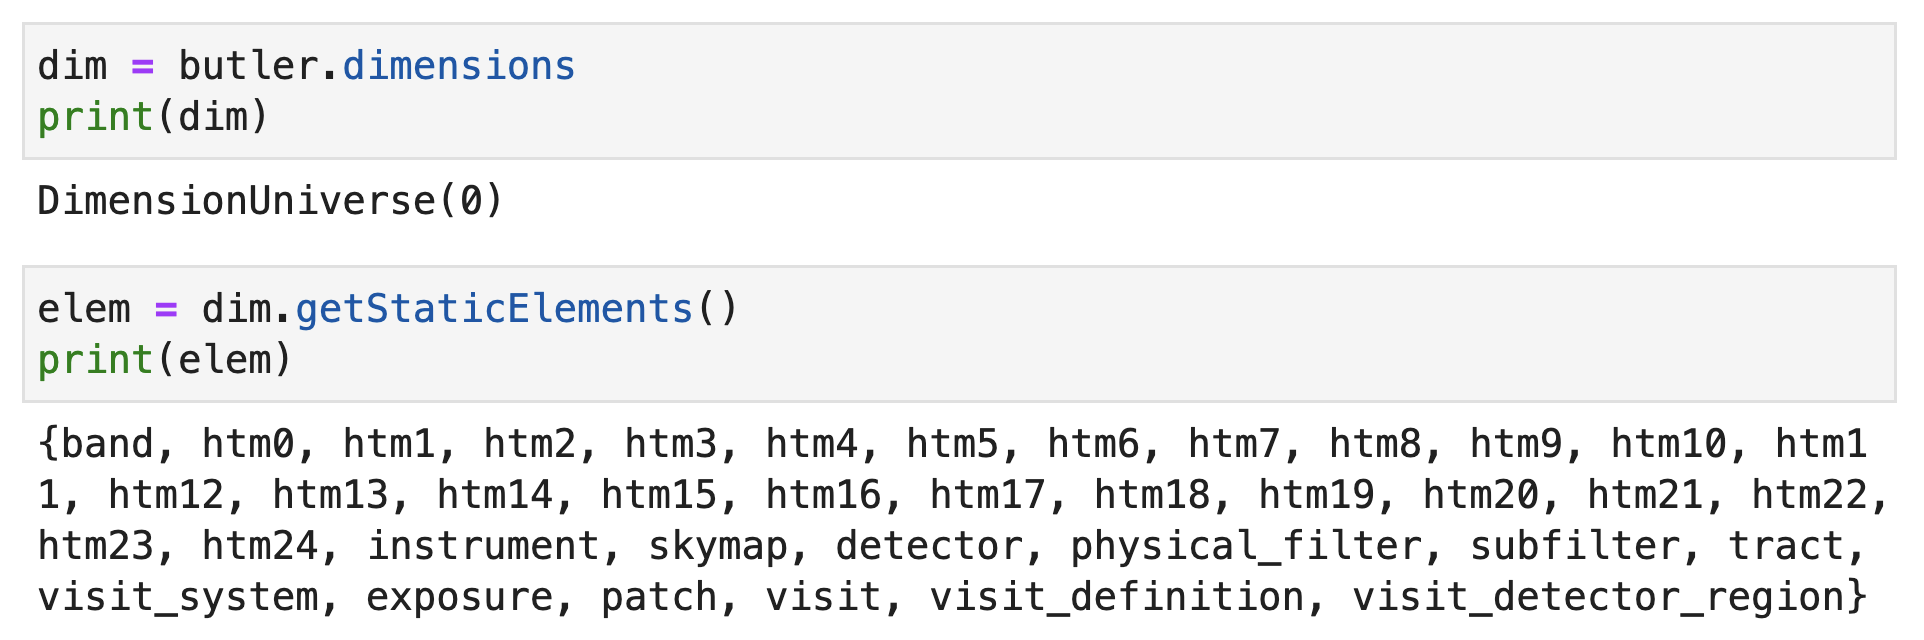
\includegraphics[width=5.07292in]{jira_imgs/2385.png}\\
Now, we illustrate that each of those `StaticElements` have
``column-like'' things within them that can be exposed via
`RecordClass.fields`:\\[2\baselineskip]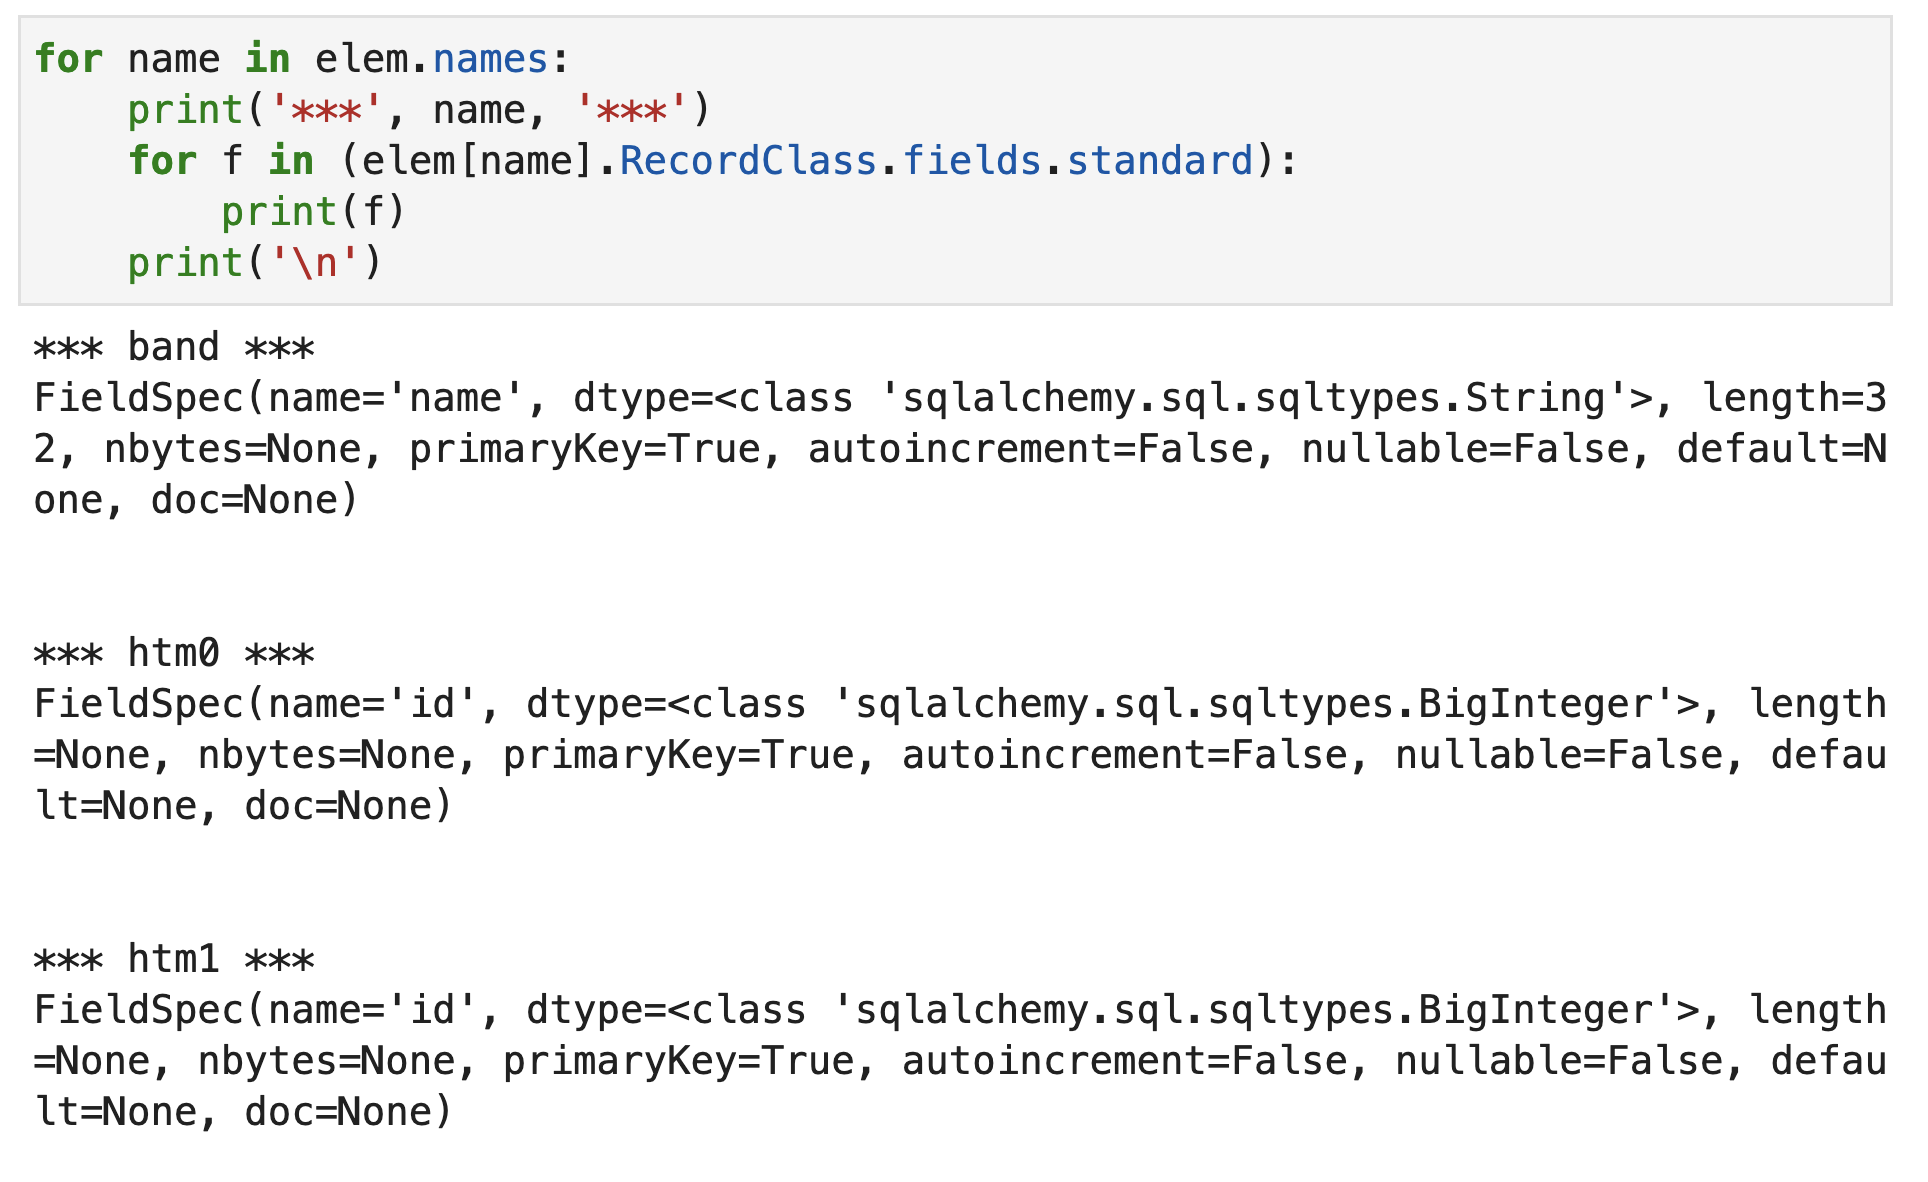
\includegraphics[width=5.17708in]{jira_imgs/2386.png}The
first few elements in the list are fairly simple, and we have truncated
the list for brevity. For illustration, here is an element (``visit'')
with a more complex set of fields:\\
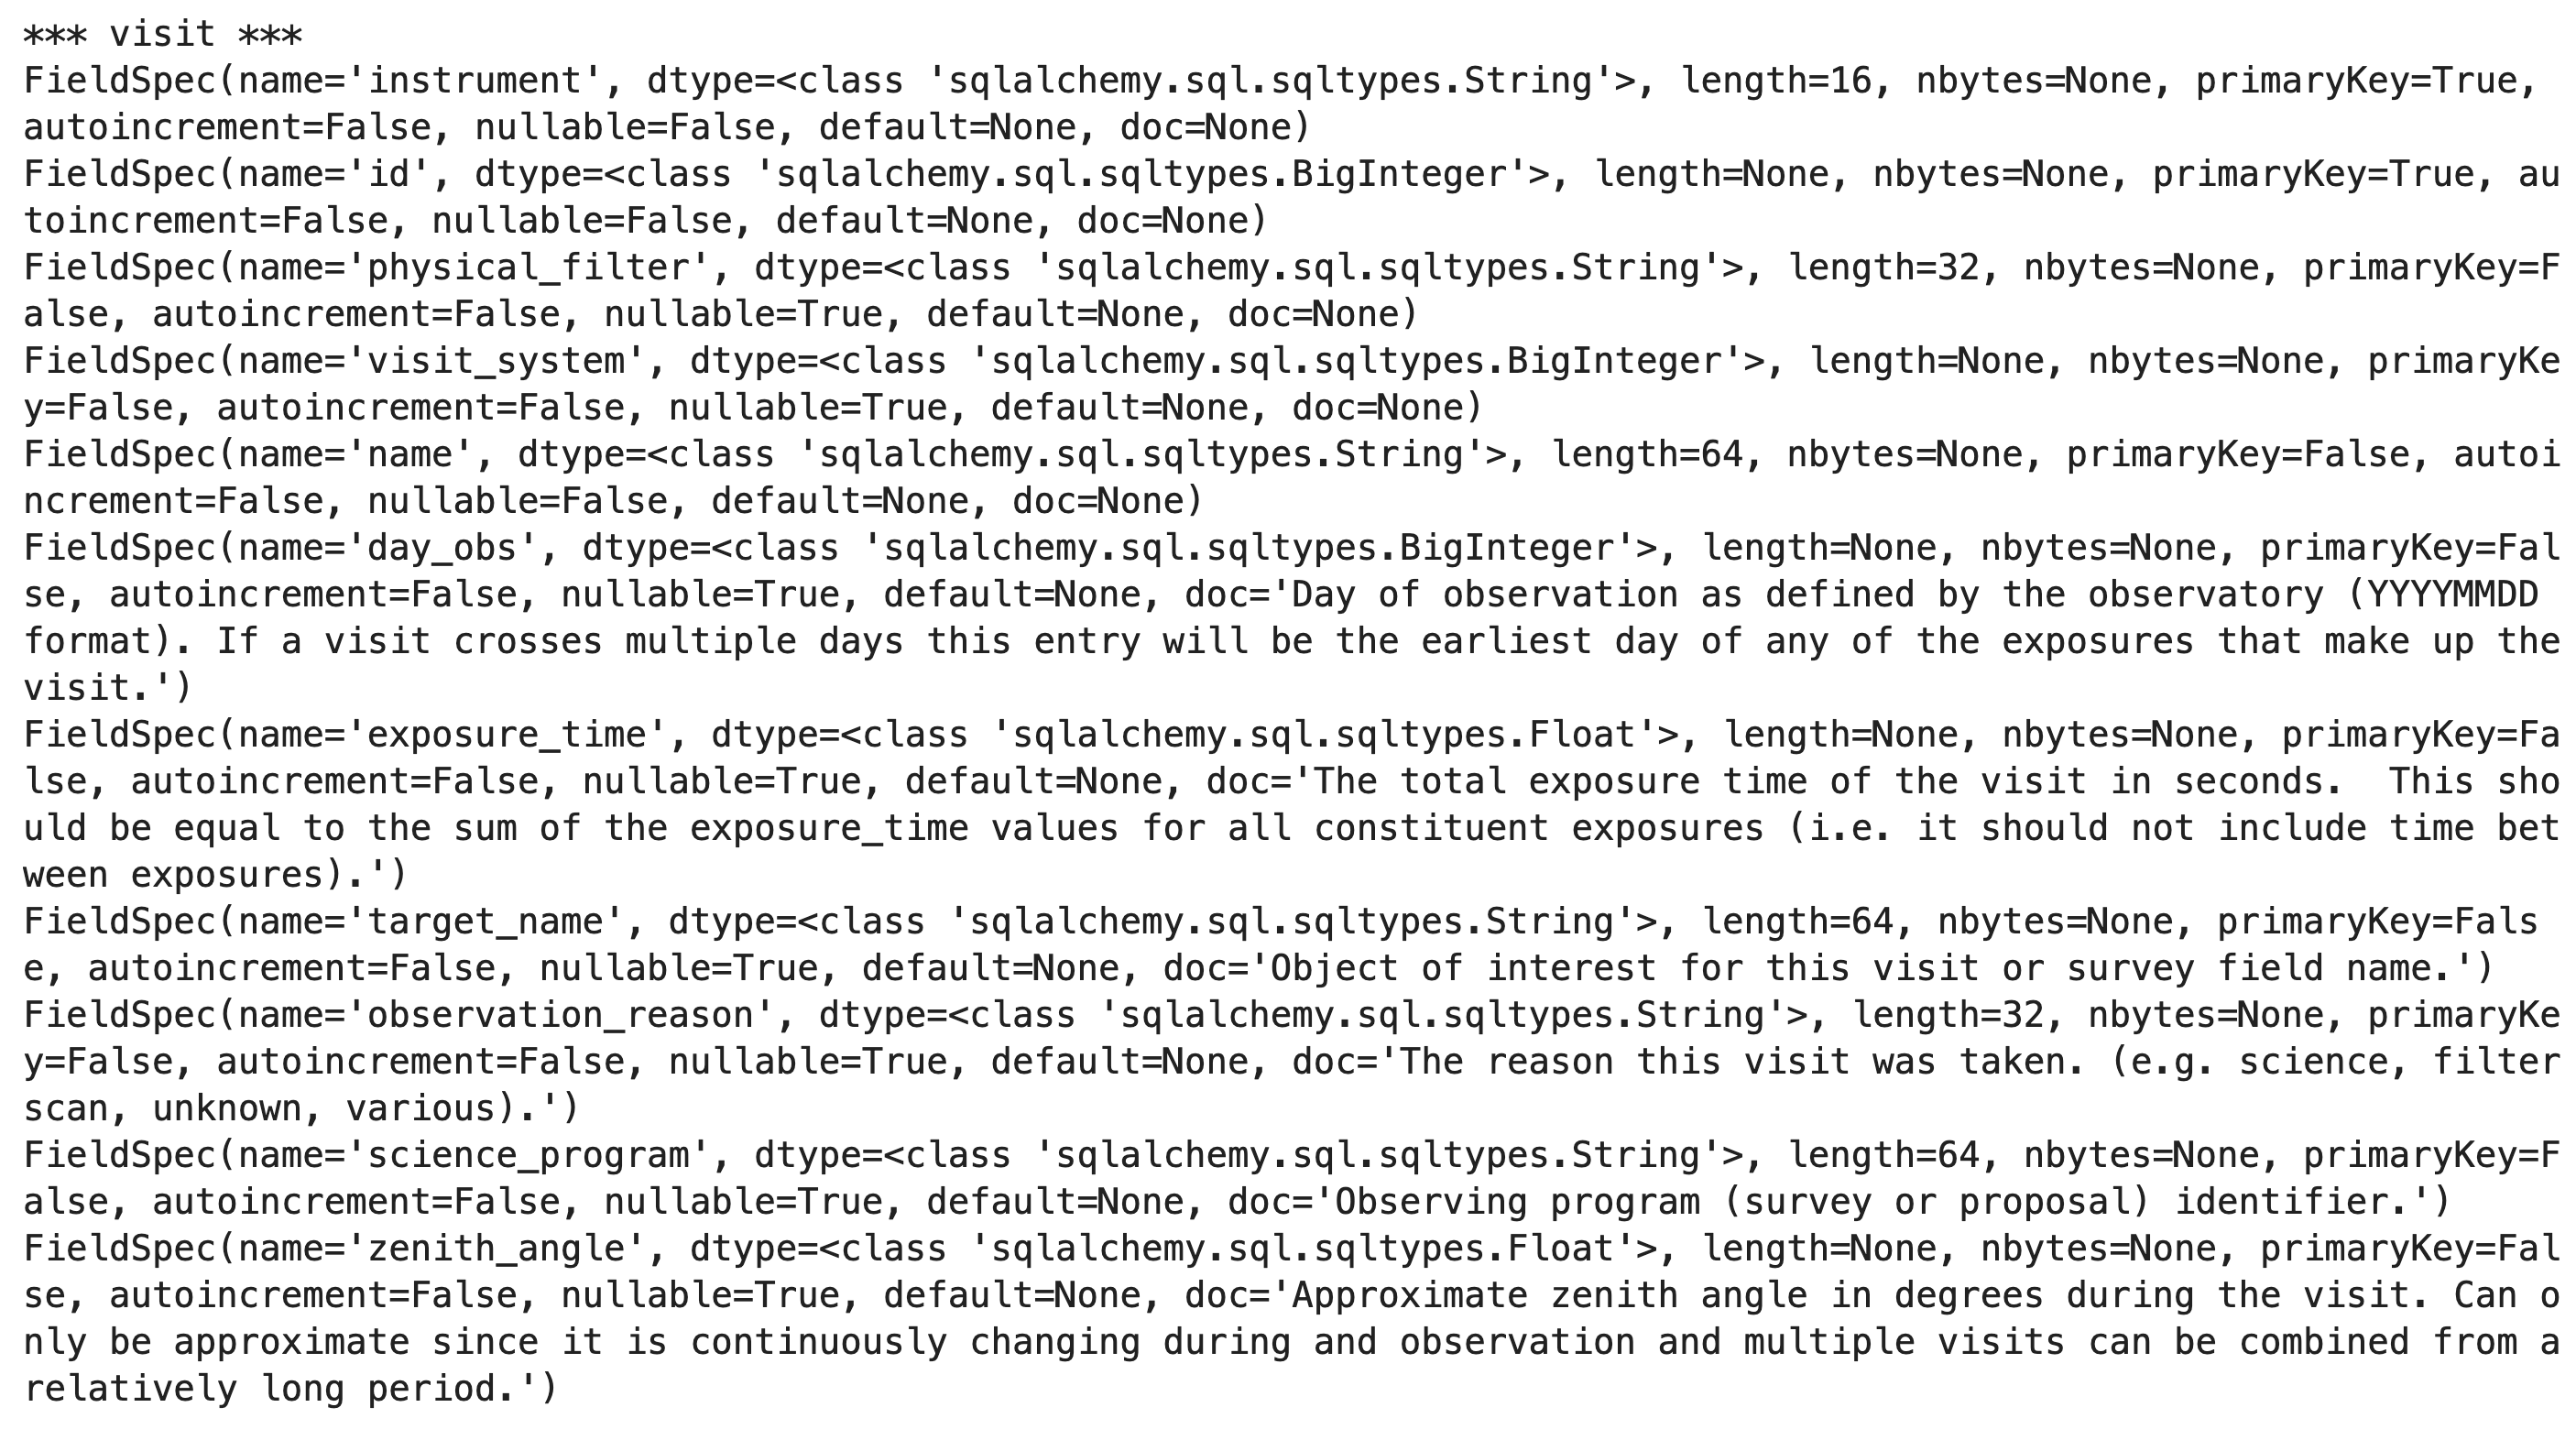
\includegraphics[width=6.05208in]{jira_imgs/2387.png}\\
We have thus demonstrated the capability of exposing a DataRepository's
schema in order that DatasetExpressions could be constructed.

}

\paragraph{ LVV-T2471 - Verify Filter by non-DatasetRef Database Entries }\mbox{}\\

Version \textbf{1}.
Open  \href{https://jira.lsstcorp.org/secure/Tests.jspa#/testCase/LVV-T2471}{\textit{ LVV-T2471 } }
test case in Jira.

Verify that the Data Discovery System is able to filter search results
based upon specified filters that need non-DatasetRef database entries

\textbf{ Preconditions}:\\


Execution status: {\bf Pass }

Final comment:\\


Detailed steps results:

\begin{tabular}{p{2cm}p{14cm}}
\toprule
Step 1 & Step Execution Status: \textbf{ Pass } \\ \hline
\end{tabular}
 Description \\
{\footnotesize
Run `butler query-datasets` against any major repo (e.g. `/repo/main`),
with a WHERE expression involving some dimension metadata fields.

}
\hdashrule[0.5ex]{\textwidth}{1pt}{3mm}
  Expected Result \\
{\footnotesize

}
\hdashrule[0.5ex]{\textwidth}{1pt}{3mm}
  Actual Result \\
{\footnotesize
We demonstrate this using the same query as in LVV-T2467. This query
includes a ``WHERE'' clause to select `calexp` datasets based on tract
and patch criteria. Because tract/patch are not dimensions of a
`calexp`, this demonstrates the use of dimension metadata for
selection.\\[2\baselineskip]butler query-datasets /repo/main calexp
--where ``tract=9615 AND patch=43 AND skymap='hsc\_rings\_v1'''
--collections HSC/runs/RC2/w\_2022\_12/DM-34125 \textbar{}
less\\[2\baselineskip]The first few lines of the returned table are
captured in this screenshot:\\
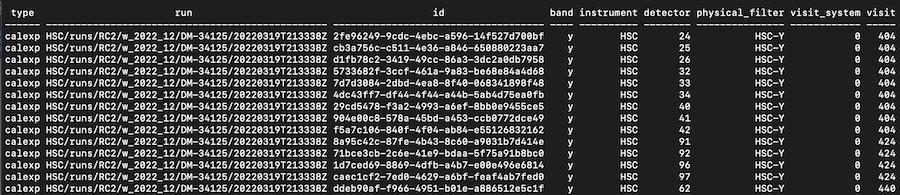
\includegraphics[width=7.16667in]{jira_imgs/2314.png}\\[2\baselineskip]This
demonstrates the use of dimension metadata for filtering search results
from the butler.

}

\paragraph{ LVV-T2470 - Verify Dataset overrides }\mbox{}\\

Version \textbf{1}.
Open  \href{https://jira.lsstcorp.org/secure/Tests.jspa#/testCase/LVV-T2470}{\textit{ LVV-T2470 } }
test case in Jira.

Verify that it is possible for an operator to configure the Data
Discovery System to override certain Datasets with others before
retrieval.

\textbf{ Preconditions}:\\


Execution status: {\bf Pass }

Final comment:\\We verify this with the same query as used in LVV-T2469, but instead
specifying ``findFirst=True'' to override the default behavior.


Detailed steps results:

\begin{tabular}{p{2cm}p{14cm}}
\toprule
Step 1 & Step Execution Status: \textbf{ Pass } \\ \hline
\end{tabular}
 Description \\
{\footnotesize
Run `butler query-datasets` against any major repo (e.g. `/repo/main`),
with multiple input collections that contain the same unresolved
DatasetRefs, with findFirst=True.

}
\hdashrule[0.5ex]{\textwidth}{1pt}{3mm}
  Expected Result \\
{\footnotesize

}
\hdashrule[0.5ex]{\textwidth}{1pt}{3mm}
  Actual Result \\
{\footnotesize
butler query-datasets /repo/main deepCoadd\_calexp --collections
HSC/runs/RC2/w\_2022\_12/DM-34125,HSC/runs/RC2/w\_2022\_08/DM-33741
--where ``tract=9615 AND patch=43 AND band='i' AND
skymap='hsc\_rings\_v1'''
--find-first\\[2\baselineskip]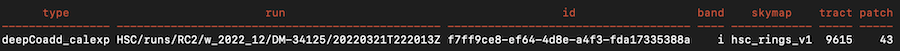
\includegraphics[width=6.60417in]{jira_imgs/2319.png}\\
As expected, this query returns a single result -- the ``first.''

}

\paragraph{ LVV-T2469 - Verify Multiple parallel input Collections }\mbox{}\\

Version \textbf{1}.
Open  \href{https://jira.lsstcorp.org/secure/Tests.jspa#/testCase/LVV-T2469}{\textit{ LVV-T2469 } }
test case in Jira.

Verify that the Data Discovery System is able to locate Datasets from
multiple input Collections in order to retrieve the same logical Dataset
from them all.\\[2\baselineskip]This is to allow for comparison of the
same data reduced with multiple different stacks.

\textbf{ Preconditions}:\\


Execution status: {\bf Pass }

Final comment:\\We verify this by demonstrating that a `deepCoadd\_calexp` can be
retrieved for the same tract, patch, band combination, but from
different collections (i.e., data processed with different pipeline
versions).


Detailed steps results:

\begin{tabular}{p{2cm}p{14cm}}
\toprule
Step 1 & Step Execution Status: \textbf{ Pass } \\ \hline
\end{tabular}
 Description \\
{\footnotesize
Run `butler query-datasets` against any major repo (e.g. `/repo/main`),
with multiple input collections that contain the same unresolved
DatasetRefs, with findFirst=False

}
\hdashrule[0.5ex]{\textwidth}{1pt}{3mm}
  Expected Result \\
{\footnotesize

}
\hdashrule[0.5ex]{\textwidth}{1pt}{3mm}
  Actual Result \\
{\footnotesize
butler query-datasets /repo/main deepCoadd\_calexp --collections
HSC/runs/RC2/w\_2022\_12/DM-34125,HSC/runs/RC2/w\_2022\_08/DM-33741
--where ``tract=9615 AND patch=43 AND band='i' AND
skymap='hsc\_rings\_v1'''\\[2\baselineskip]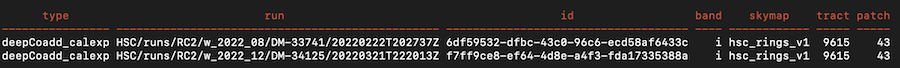
\includegraphics[width=6.48958in]{jira_imgs/2318.png}\\
This demonstrates that the butler can identify the same logical Dataset
(`deepCoadd\_calexp`) from different collections in the same query.

}

\paragraph{ LVV-T2468 - Verify Multiple chained input Collections }\mbox{}\\

Version \textbf{1}.
Open  \href{https://jira.lsstcorp.org/secure/Tests.jspa#/testCase/LVV-T2468}{\textit{ LVV-T2468 } }
test case in Jira.

Verify that the ~Data Discovery System is able treat multiple input
Collections as a single coherent logical repository

\textbf{ Preconditions}:\\


Execution status: {\bf Pass }

Final comment:\\


Detailed steps results:

\begin{tabular}{p{2cm}p{14cm}}
\toprule
Step 1 & Step Execution Status: \textbf{ Pass } \\ \hline
\end{tabular}
 Description \\
{\footnotesize
Run `butler query-datasets` against any major repo (e.g `repo/main`)
with multiple input collections.

}
\hdashrule[0.5ex]{\textwidth}{1pt}{3mm}
  Expected Result \\
{\footnotesize

}
\hdashrule[0.5ex]{\textwidth}{1pt}{3mm}
  Actual Result \\
{\footnotesize
This will be demonstrated by showing that datasets of type
`objectTable\_tract` can be retrieved by a butler query from multiple
collections.\\[2\baselineskip]Execute the following query to retrieve
`objectTable\_tract` from RC2 reprocessing collections corresponding to
weekly pipelines from w\_2022\_08 and
w\_2022\_12:\\[2\baselineskip]butler query-datasets /repo/main
objectTable\_tract --collections
HSC/runs/RC2/w\_2022\_12/DM-34125,HSC/runs/RC2/w\_2022\_08/DM-33741\\[2\baselineskip]This
returns the following table:\\
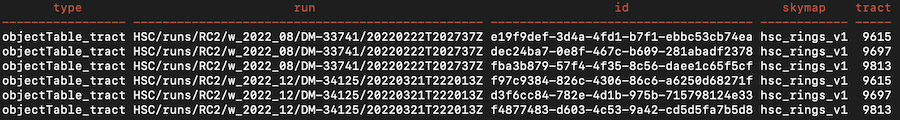
\includegraphics[width=5.63542in]{jira_imgs/2315.png}\\
We have thus demonstrated that datasets from multiple collections can be
retrieved by the butler as a single coherent unit.\\[2\baselineskip]

}

\paragraph{ LVV-T2466 - Verify enable complete pipeline specification }\mbox{}\\

Version \textbf{1}.
Open  \href{https://jira.lsstcorp.org/secure/Tests.jspa#/testCase/LVV-T2466}{\textit{ LVV-T2466 } }
test case in Jira.

Verify that the design provides an interface for delivering a complete
algorithmic work specification (a ``Pipeline specification'') from
Science Pipelines to an execution system, the ``supervisory framework'',
a notable instance of which is the LSST production system.

\textbf{ Preconditions}:\\


Execution status: {\bf Pass }

Final comment:\\


Detailed steps results:

\begin{tabular}{p{2cm}p{14cm}}
\toprule
Step 1 & Step Execution Status: \textbf{ Pass } \\ \hline
\end{tabular}
 Description \\
{\footnotesize
This is a fundamental part of the design of PipelineTask.

}
\hdashrule[0.5ex]{\textwidth}{1pt}{3mm}
  Expected Result \\
{\footnotesize

}
\hdashrule[0.5ex]{\textwidth}{1pt}{3mm}
  Actual Result \\
{\footnotesize
As an example of a full pipeline specification, we inspect
\href{https://github.com/lsst/drp_pipe/blob/main/pipelines/HSC/DRP-RC2.yaml}{DRP-RC2.yaml},
which is the pipeline used for end-to-end processing of the RC2 dataset.
The screenshot below shows a portion of DRP-RC2.yaml, in which subsets
(``step1'' and ``step2'') of sequential pipelineTasks are
specified:\\[2\baselineskip]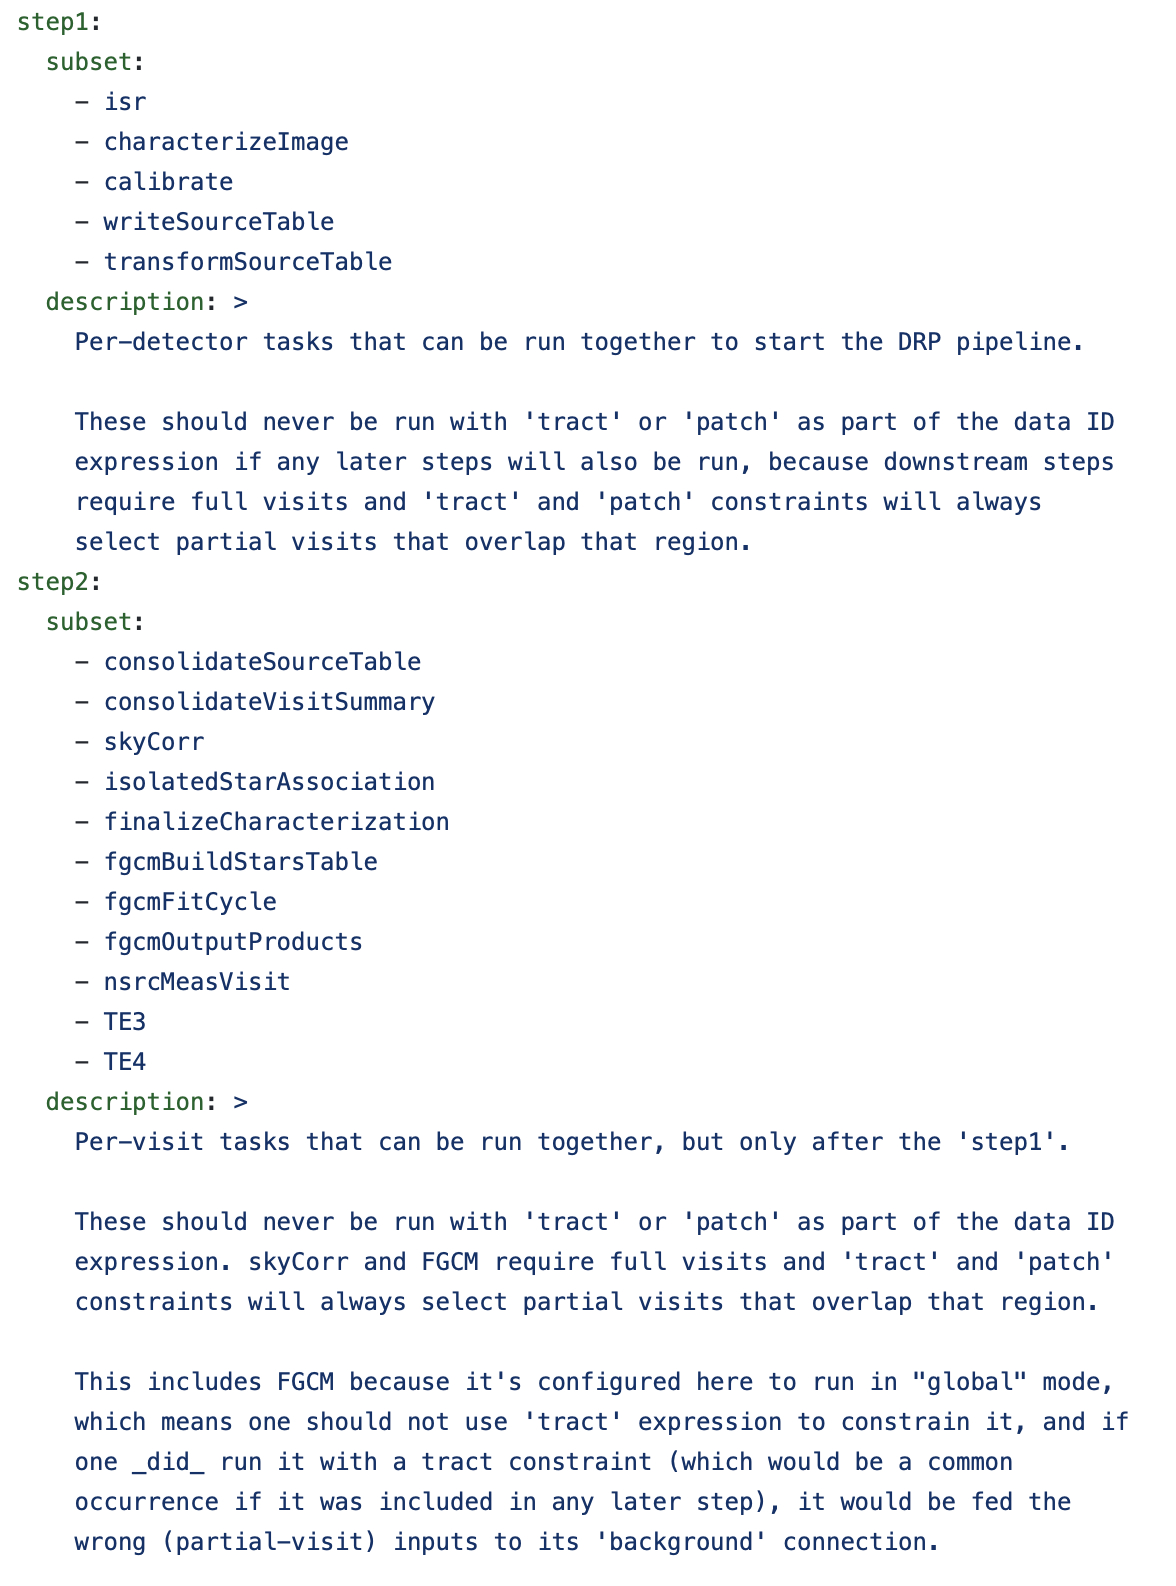
\includegraphics[width=4.77083in]{jira_imgs/2413.png}By
inspection (and the knowledge that this pipeline is regularly executed
in campaigns such as that described in
\href{https://jira.lsstcorp.org/browse/DM-34451}{DM-34451}), we have
thus verified that a complete algorithmic work specification can be
delivered to an execution system.

}

\paragraph{ LVV-T2467 - Verify DataUnit lookup: processing driven }\mbox{}\\

Version \textbf{1}.
Open  \href{https://jira.lsstcorp.org/secure/Tests.jspa#/testCase/LVV-T2467}{\textit{ LVV-T2467 } }
test case in Jira.

Verify that all Data Discovery Systems ~make it possible to discover the
DataUnits for all Datasets that could potentially be used to produce a
given DatasetType with known DataUnits.

\textbf{ Preconditions}:\\


Execution status: {\bf Pass }

Final comment:\\We will verify this by demonstrating that all dataset overlapping a
given tract/patch combination (and thus a specific sky region) can be
readily discovered.~


Detailed steps results:

\begin{tabular}{p{2cm}p{14cm}}
\toprule
Step 1 & Step Execution Status: \textbf{ Pass } \\ \hline
\end{tabular}
 Description \\
{\footnotesize
Run `butler query-datasets` against any major repo (e.g. `/repo/main`).

}
\hdashrule[0.5ex]{\textwidth}{1pt}{3mm}
  Expected Result \\
{\footnotesize

}
\hdashrule[0.5ex]{\textwidth}{1pt}{3mm}
  Actual Result \\
{\footnotesize
This query returns a list of all `calexp` datasets overlapping an
arbitrarily chosen tract (known a priori to contain data in the HSC RC2
dataset), patch combination (9615, 43).\\[2\baselineskip]butler
query-datasets /repo/main calexp --where ``tract=9615 AND patch=43 AND
skymap='hsc\_rings\_v1''' --collections
HSC/runs/RC2/w\_2022\_12/DM-34125 \textbar{} less\\[2\baselineskip]The
first few lines of the returned table are captured in this screenshot:\\
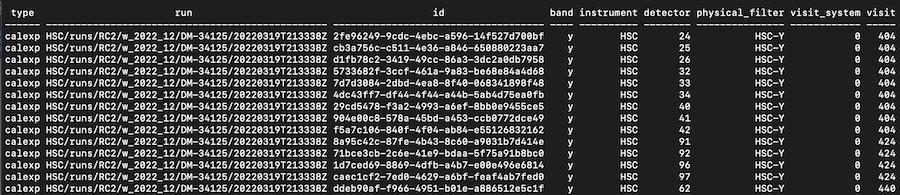
\includegraphics[width=4.79167in]{jira_imgs/2314.png}\\
We have thus demonstrated that dataset discovery by a given set of
DataUnits is enabled by the butler.

}

\paragraph{ LVV-T2464 - Verify multiple simultaneous sky definitions }\mbox{}\\

Version \textbf{1}.
Open  \href{https://jira.lsstcorp.org/secure/Tests.jspa#/testCase/LVV-T2464}{\textit{ LVV-T2464 } }
test case in Jira.

Verify that a collection is able to hold Datasets corresponding to
different sky tilings simultaneously\\[2\baselineskip]

\textbf{ Preconditions}:\\


Execution status: {\bf Pass }

Final comment:\\


Detailed steps results:

\begin{tabular}{p{2cm}p{14cm}}
\toprule
Step 1 & Step Execution Status: \textbf{ Pass } \\ \hline
\end{tabular}
 Description \\
{\footnotesize
Make empty repo.

}
\hdashrule[0.5ex]{\textwidth}{1pt}{3mm}
  Expected Result \\
{\footnotesize

}
\hdashrule[0.5ex]{\textwidth}{1pt}{3mm}
  Actual Result \\
{\footnotesize

}
\begin{tabular}{p{2cm}p{14cm}}
\toprule
Step 2 & Step Execution Status: \textbf{ Pass } \\ \hline
\end{tabular}
 Description \\
{\footnotesize
Run `butler register-skymap`.

}
\hdashrule[0.5ex]{\textwidth}{1pt}{3mm}
  Expected Result \\
{\footnotesize

}
\hdashrule[0.5ex]{\textwidth}{1pt}{3mm}
  Actual Result \\
{\footnotesize

}
\begin{tabular}{p{2cm}p{14cm}}
\toprule
Step 3 & Step Execution Status: \textbf{ Pass } \\ \hline
\end{tabular}
 Description \\
{\footnotesize
Run `butler register-skymap` a second time

}
\hdashrule[0.5ex]{\textwidth}{1pt}{3mm}
  Expected Result \\
{\footnotesize

}
\hdashrule[0.5ex]{\textwidth}{1pt}{3mm}
  Actual Result \\
{\footnotesize
We will start with an existing repository that has more than one
existing skymap. In particular, we will select a repo with recent
reprocessing of the RC2 dataset.

}
\begin{tabular}{p{2cm}p{14cm}}
\toprule
Step 4 & Step Execution Status: \textbf{ Pass } \\ \hline
\end{tabular}
 Description \\
{\footnotesize
Verify that mappings to both tile definitions are valid

}
\hdashrule[0.5ex]{\textwidth}{1pt}{3mm}
  Expected Result \\
{\footnotesize

}
\hdashrule[0.5ex]{\textwidth}{1pt}{3mm}
  Actual Result \\
{\footnotesize
On lsst-devl at NCSA, with the science pipelines set up, opened python
and typed the following:\\[2\baselineskip]import lsst.daf.butler as
dafButler\\
repo =~``/repo/main''\\
butler = dafButler.Butler(repo,
collections={[}``HSC/runs/RC2/w\_2022\_12/DM-34125''{]})\\
registry = butler.registry\\
for d~in registry.queryDimensionRecords(``skymap''):\\
\hspace*{0.333em} ~ print(d)\\[2\baselineskip]This results in the
following screen output:\\[2\baselineskip]skymap:\\
\hspace*{0.333em}\hspace*{0.333em}name: `hsc\_rings\_v1'\\
\hspace*{0.333em}\hspace*{0.333em}hash:
b'\textbackslash{}xe2\textbackslash{}x9f\textbackslash{}xe9\textbackslash{}xf1\textbackslash{}x00\textbackslash{}x8e5\textbackslash{}x9f6\textbackslash{}xa3g\textasciitilde{}\}i\textbackslash{}xccC\textbackslash{}x93v\textbackslash{}xd1\textbackslash{}xe6'\\
\hspace*{0.333em}\hspace*{0.333em}tract\_max: 18938\\
\hspace*{0.333em}\hspace*{0.333em}patch\_nx\_max: 9\\
\hspace*{0.333em}\hspace*{0.333em}patch\_ny\_max: 9\\
skymap:\\
\hspace*{0.333em}\hspace*{0.333em}name: `hsc\_rings\_cells\_v1'\\
\hspace*{0.333em}\hspace*{0.333em}hash:
b'\textbackslash{}xde\textbackslash{}x85\textbackslash{}x13\textbackslash{}xb0q\textbackslash{}x11\textbackslash{}x1e\textbackslash{}x81a\textbackslash{}x9e\textbackslash{}\textbackslash{}\textbackslash{}x06\textbackslash{}x1f\textbackslash{}x02mA\textbackslash{}xf7h\textbackslash{}xe6\textbackslash{}xd4'\\
\hspace*{0.333em}\hspace*{0.333em}tract\_max: 18938\\
\hspace*{0.333em}\hspace*{0.333em}patch\_nx\_max: 11\\
\hspace*{0.333em} patch\_ny\_max: 11\\[2\baselineskip]This demonstrates
that this single collection (``HSC/runs/RC2/w\_2022\_12/DM-34125'')
contains two sky maps with different numbers of patches (i.e., with
different values of patch\_nx\_max and patch\_ny\_max).

}

\paragraph{ LVV-T2465 - Verify pipeline execution in multiple contexts }\mbox{}\\

Version \textbf{1}.
Open  \href{https://jira.lsstcorp.org/secure/Tests.jspa#/testCase/LVV-T2465}{\textit{ LVV-T2465 } }
test case in Jira.

Verify that the design allows a given Pipeline specification to be used
in both development and production contexts.

\textbf{ Preconditions}:\\


Execution status: {\bf Pass }

Final comment:\\


Detailed steps results:

\begin{tabular}{p{2cm}p{14cm}}
\toprule
Step 1 & Step Execution Status: \textbf{ Pass } \\ \hline
\end{tabular}
 Description \\
{\footnotesize
This is a fundamental part of the design of PipelineTask.

}
\hdashrule[0.5ex]{\textwidth}{1pt}{3mm}
  Expected Result \\
{\footnotesize

}
\hdashrule[0.5ex]{\textwidth}{1pt}{3mm}
  Actual Result \\
{\footnotesize
This is demonstrated by the fact that regular reprocessing of the RC2
dataset (using BPS) uses the same DRP pipeline as CI jobs such as
`ci\_hsc`, or small datasets such as
\href{https://github.com/lsst-dm/rc2_subset}{rc2\_subset}, which are
regularly run from the command line on lsst-devl machines for testing
purposes. For example, note that the ``DRP.yaml'' pipeline from
`rc2\_subset` imports directly from
\href{https://github.com/lsst/drp_pipe/tree/main/pipelines}{drp\_pipe},
which contains the main pipeline used for RC2 processing.

}

\paragraph{ LVV-T2461 - Verify Collection Layering: Science Platform }\mbox{}\\

Version \textbf{1}.
Open  \href{https://jira.lsstcorp.org/secure/Tests.jspa#/testCase/LVV-T2461}{\textit{ LVV-T2461 } }
test case in Jira.

Verify that collections ~created in the Science Platform are usable as
inputs for processing initiated in the Science Platform

\textbf{ Preconditions}:\\


Execution status: {\bf Not Executed }

Final comment:\\


Detailed steps results:

\begin{tabular}{p{2cm}p{14cm}}
\toprule
Step 1 & Step Execution Status: \textbf{ Not Executed } \\ \hline
\end{tabular}
 Description \\
{\footnotesize
Run part of DRP pipeline in RSP.

}
\hdashrule[0.5ex]{\textwidth}{1pt}{3mm}
  Expected Result \\
{\footnotesize

}
\hdashrule[0.5ex]{\textwidth}{1pt}{3mm}
  Actual Result \\
{\footnotesize

}
\begin{tabular}{p{2cm}p{14cm}}
\toprule
Step 2 & Step Execution Status: \textbf{ Not Executed } \\ \hline
\end{tabular}
 Description \\
{\footnotesize
Run a later part of DRP pipeline in RSP

}
\hdashrule[0.5ex]{\textwidth}{1pt}{3mm}
  Expected Result \\
{\footnotesize

}
\hdashrule[0.5ex]{\textwidth}{1pt}{3mm}
  Actual Result \\
{\footnotesize

}

\paragraph{ LVV-T2463 - Verify enabling of different execution environments }\mbox{}\\

Version \textbf{1}.
Open  \href{https://jira.lsstcorp.org/secure/Tests.jspa#/testCase/LVV-T2463}{\textit{ LVV-T2463 } }
test case in Jira.

Verify that the supervisory framework supports the creation of multiple
specializations for different execution environments.

\textbf{ Preconditions}:\\


Execution status: {\bf Pass }

Final comment:\\


Detailed steps results:

\begin{tabular}{p{2cm}p{14cm}}
\toprule
Step 1 & Step Execution Status: \textbf{ Pass } \\ \hline
\end{tabular}
 Description \\
{\footnotesize
Satisfied by BPS plugin system; we have plugins for many workflow
systems already.

}
\hdashrule[0.5ex]{\textwidth}{1pt}{3mm}
  Expected Result \\
{\footnotesize

}
\hdashrule[0.5ex]{\textwidth}{1pt}{3mm}
  Actual Result \\
{\footnotesize
By examination of the
\href{https://github.com/lsst/lsst_bps_plugins}{lsst\_bps\_plugins}
package, which is a metapackage containing all of the various BPS
plugins for the LSST Science Pipelines, we confirm that this requirement
is met. Currently the
\href{https://github.com/lsst/ctrl_bps_panda}{ctrl\_bps\_panda} plugin
is being used for DP0.2 processing at the IDF, and
\href{https://github.com/lsst/ctrl_bps_htcondor}{ctrl\_bps\_htcondor} is
used for regular RC2 and DC2 reprocessing campaigns (see, e.g.,
\href{https://jira.lsstcorp.org/browse/DM-34451}{Jira ticket
DM-34451}~for details of recent RC2 processing).

}

\paragraph{ LVV-T2462 - Verify QuantumGraph algorithm }\mbox{}\\

Version \textbf{1}.
Open  \href{https://jira.lsstcorp.org/secure/Tests.jspa#/testCase/LVV-T2462}{\textit{ LVV-T2462 } }
test case in Jira.

Verify QuantumGraph algorithm common to all execution environments.
Verify that the supervisory framework provides a common implementation
of the logic required for interpretation of the Pipeline steps and their
data groupings (and thus the possible parallelization); i.e., that the
QuantumGraph generation algorithm can be common to all execution
environments.

\textbf{ Preconditions}:\\


Execution status: {\bf Pass }

Final comment:\\Working on lsst-devl machines in a cloned `pipe\_base` repository at
/project/jcarlin/SVV/gen3\_middleware\_acceptance\_testing/pipe\_base


Detailed steps results:

\begin{tabular}{p{2cm}p{14cm}}
\toprule
Step 1 & Step Execution Status: \textbf{ Pass } \\ \hline
\end{tabular}
 Description \\
{\footnotesize
Execute the test\_graphBuilder.py and test\_quantumGraph.py unit tests
in the \href{https://github.com/lsst/pipe_base/}{pipe\_base}~package.

}
\hdashrule[0.5ex]{\textwidth}{1pt}{3mm}
  Expected Result \\
{\footnotesize
Successful execution of the unit tests.

}
\hdashrule[0.5ex]{\textwidth}{1pt}{3mm}
  Actual Result \\
{\footnotesize
First execute the unit test of a simple graph
builder:\\[2\baselineskip]pytest -s -vv --no-header --cache-clear
tests/test\_graphBuilder.py\\[2\baselineskip]Result:\\[2\baselineskip]tests/test\_graphBuilder.py::FLAKE8~PASSED\\
tests/test\_graphBuilder.py::GraphBuilderTestCase::testAddInstrumentMismatch~PASSED\\
tests/test\_graphBuilder.py::GraphBuilderTestCase::testDefault
PASSED\\[2\baselineskip]Now execute the unit test that more thoroughly
tests quantum graph generation and usage:\\
pytest -s -vv --no-header --cache-clear tests/test\_quantumGraph.py
\textbar{} tee
test\_QG\_log.txt\\[2\baselineskip]tests/test\_quantumGraph.py::FLAKE8
PASSED\\
tests/test\_quantumGraph.py::QuantumGraphTestCase::testAllDatasetTypes
PASSED\\
tests/test\_quantumGraph.py::QuantumGraphTestCase::testContains PASSED\\
tests/test\_quantumGraph.py::QuantumGraphTestCase::testDetermineAnsestorsOfQuantumNode
PASSED\\
tests/test\_quantumGraph.py::QuantumGraphTestCase::testDetermineConnectionsOfQuantum
PASSED\\
tests/test\_quantumGraph.py::QuantumGraphTestCase::testDetermineOutputsOfQuantumNode
PASSED\\
tests/test\_quantumGraph.py::QuantumGraphTestCase::testFindCycle
PASSED\\
tests/test\_quantumGraph.py::QuantumGraphTestCase::testFindQuantaWIthDSType
PASSED\\
tests/test\_quantumGraph.py::QuantumGraphTestCase::testFindTaskDefByLabel
PASSED\\
tests/test\_quantumGraph.py::QuantumGraphTestCase::testFindTaskDefByName
PASSED\\
tests/test\_quantumGraph.py::QuantumGraphTestCase::testFindTasksWithInput
PASSED\\
tests/test\_quantumGraph.py::QuantumGraphTestCase::testFindTasksWithOutput
PASSED\\
tests/test\_quantumGraph.py::QuantumGraphTestCase::testGetNodesForTask
PASSED\\
tests/test\_quantumGraph.py::QuantumGraphTestCase::testGetQuantaForTask
PASSED\\
tests/test\_quantumGraph.py::QuantumGraphTestCase::testGetQuantumNodeByNodeId
PASSED\\
tests/test\_quantumGraph.py::QuantumGraphTestCase::testGraph PASSED\\
tests/test\_quantumGraph.py::QuantumGraphTestCase::testInputQuanta
PASSED\\
tests/test\_quantumGraph.py::QuantumGraphTestCase::testLength PASSED\\
tests/test\_quantumGraph.py::QuantumGraphTestCase::testOutputtQuanta
PASSED\\
tests/test\_quantumGraph.py::QuantumGraphTestCase::testPickle PASSED\\
tests/test\_quantumGraph.py::QuantumGraphTestCase::testSaveLoad PASSED\\
tests/test\_quantumGraph.py::QuantumGraphTestCase::testSaveLoadUri
PASSED\\
tests/test\_quantumGraph.py::QuantumGraphTestCase::testSaveLoadUriS3
PASSED\\
tests/test\_quantumGraph.py::QuantumGraphTestCase::testSubset PASSED\\
tests/test\_quantumGraph.py::QuantumGraphTestCase::testSubsetToConnected
PASSED\\
tests/test\_quantumGraph.py::QuantumGraphTestCase::testTaskGraph
PASSED\\
tests/test\_quantumGraph.py::QuantumGraphTestCase::testTaskWithDSType
PASSED\\
tests/test\_quantumGraph.py::MyMemoryTestCase::testFileDescriptorLeaks
\textless{}-
../../../../../software/lsstsw/stack\_20220215/stack/miniconda3-py38\_4.9.2-2.0.0/Linux64/utils/g617c0b0dc2+9633a190c8/python/lsst/utils/tests.py
PASSED\\[2\baselineskip]All passed. This demonstrates that functional
code is in place for generating quantum graphs.\\[2\baselineskip]

}

\paragraph{ LVV-T2460 - Verify generating a DAG }\mbox{}\\

Version \textbf{1}.
Open  \href{https://jira.lsstcorp.org/secure/Tests.jspa#/testCase/LVV-T2460}{\textit{ LVV-T2460 } }
test case in Jira.

Verify that the supervisory framework supports the ``Pre-flight'' phase
of execution of a Pipeline on a specified set of inputs and/or desired
outputs, resulting in a Directed Acyclic Graph (DAG) for the processing,
with the nodes in the DAG being the units of work to be executed.

\textbf{ Preconditions}:\\


Execution status: {\bf Pass }

Final comment:\\Working on lsst-devl machines in a cloned `pipe\_base` repository
at~/project/jcarlin/SVV/gen3\_middleware\_acceptance\_testing/pipe\_base


Detailed steps results:

\begin{tabular}{p{2cm}p{14cm}}
\toprule
Step 1 & Step Execution Status: \textbf{ Pass } \\ \hline
\end{tabular}
 Description \\
{\footnotesize
Satisfied by existence of QuantumGraph generation code.

}
\hdashrule[0.5ex]{\textwidth}{1pt}{3mm}
  Expected Result \\
{\footnotesize

}
\hdashrule[0.5ex]{\textwidth}{1pt}{3mm}
  Actual Result \\
{\footnotesize
First execute the unit test of a simple graph
builder:\\[2\baselineskip]pytest -s -vv --no-header --cache-clear
tests/test\_graphBuilder.py\\[2\baselineskip]Result:\\[2\baselineskip]tests/test\_graphBuilder.py::FLAKE8~PASSED\\
tests/test\_graphBuilder.py::GraphBuilderTestCase::testAddInstrumentMismatch~PASSED\\
tests/test\_graphBuilder.py::GraphBuilderTestCase::testDefault
PASSED\\[2\baselineskip]Now execute the unit test that more thoroughly
tests quantum graph generation and usage:\\
pytest -s -vv --no-header --cache-clear tests/test\_quantumGraph.py
\textbar{} tee
test\_QG\_log.txt\\[2\baselineskip]tests/test\_quantumGraph.py::FLAKE8
PASSED\\
tests/test\_quantumGraph.py::QuantumGraphTestCase::testAllDatasetTypes
PASSED\\
tests/test\_quantumGraph.py::QuantumGraphTestCase::testContains PASSED\\
tests/test\_quantumGraph.py::QuantumGraphTestCase::testDetermineAnsestorsOfQuantumNode
PASSED\\
tests/test\_quantumGraph.py::QuantumGraphTestCase::testDetermineConnectionsOfQuantum
PASSED\\
tests/test\_quantumGraph.py::QuantumGraphTestCase::testDetermineOutputsOfQuantumNode
PASSED\\
tests/test\_quantumGraph.py::QuantumGraphTestCase::testFindCycle
PASSED\\
tests/test\_quantumGraph.py::QuantumGraphTestCase::testFindQuantaWIthDSType
PASSED\\
tests/test\_quantumGraph.py::QuantumGraphTestCase::testFindTaskDefByLabel
PASSED\\
tests/test\_quantumGraph.py::QuantumGraphTestCase::testFindTaskDefByName
PASSED\\
tests/test\_quantumGraph.py::QuantumGraphTestCase::testFindTasksWithInput
PASSED\\
tests/test\_quantumGraph.py::QuantumGraphTestCase::testFindTasksWithOutput
PASSED\\
tests/test\_quantumGraph.py::QuantumGraphTestCase::testGetNodesForTask
PASSED\\
tests/test\_quantumGraph.py::QuantumGraphTestCase::testGetQuantaForTask
PASSED\\
tests/test\_quantumGraph.py::QuantumGraphTestCase::testGetQuantumNodeByNodeId
PASSED\\
tests/test\_quantumGraph.py::QuantumGraphTestCase::testGraph PASSED\\
tests/test\_quantumGraph.py::QuantumGraphTestCase::testInputQuanta
PASSED\\
tests/test\_quantumGraph.py::QuantumGraphTestCase::testLength PASSED\\
tests/test\_quantumGraph.py::QuantumGraphTestCase::testOutputtQuanta
PASSED\\
tests/test\_quantumGraph.py::QuantumGraphTestCase::testPickle PASSED\\
tests/test\_quantumGraph.py::QuantumGraphTestCase::testSaveLoad PASSED\\
tests/test\_quantumGraph.py::QuantumGraphTestCase::testSaveLoadUri
PASSED\\
tests/test\_quantumGraph.py::QuantumGraphTestCase::testSaveLoadUriS3
PASSED\\
tests/test\_quantumGraph.py::QuantumGraphTestCase::testSubset PASSED\\
tests/test\_quantumGraph.py::QuantumGraphTestCase::testSubsetToConnected
PASSED\\
tests/test\_quantumGraph.py::QuantumGraphTestCase::testTaskGraph
PASSED\\
tests/test\_quantumGraph.py::QuantumGraphTestCase::testTaskWithDSType
PASSED\\
tests/test\_quantumGraph.py::MyMemoryTestCase::testFileDescriptorLeaks
\textless{}-
../../../../../software/lsstsw/stack\_20220215/stack/miniconda3-py38\_4.9.2-2.0.0/Linux64/utils/g617c0b0dc2+9633a190c8/python/lsst/utils/tests.py
PASSED\\[2\baselineskip]All passed. This demonstrates that functional
code is in place for DAG generation.\\[2\baselineskip]

}

\paragraph{ LVV-T2457 - Verify butler instantiation }\mbox{}\\

Version \textbf{1}.
Open  \href{https://jira.lsstcorp.org/secure/Tests.jspa#/testCase/LVV-T2457}{\textit{ LVV-T2457 } }
test case in Jira.

Verify that the supervisory framework creates and supplies the Butler
required to support the I/O to be performed in the ``Run'' phase, for
each unit of work.

\textbf{ Preconditions}:\\


Execution status: {\bf Pass }

Final comment:\\More detail about I/O handling via pipetask and runQuantum can be found
by
examining~\url{https://github.com/lsst/ctrl_mpexec/blob/main/python/lsst/ctrl/mpexec/singleQuantumExecutor.py}.


Detailed steps results:

\begin{tabular}{p{2cm}p{14cm}}
\toprule
Step 1 & Step Execution Status: \textbf{ Pass } \\ \hline
\end{tabular}
 Description \\
{\footnotesize
Execute unit tests in~\\
\url{https://github.com/lsst/pipe_base/blob/main/python/lsst/pipe/base/testUtils.py},
which demonstrates that `pipetask` and the `runQuantum` method (i.e.,
the ``supervisory framework'') instantiate the butler and handles all
I/O.

}
\hdashrule[0.5ex]{\textwidth}{1pt}{3mm}
  Expected Result \\
{\footnotesize
Unit test passes.

}
\hdashrule[0.5ex]{\textwidth}{1pt}{3mm}
  Actual Result \\
{\footnotesize
On lsst-devl machines at NCSA, working in a cloned version of the
`pipe\_base` repository:\\[2\baselineskip]pytest -s -vv --no-header
--cache-clear tests/test\_testUtils.py\\[2\baselineskip]Output
includes:\\
tests/test\_testUtils.py::PipelineTaskTestSuite::testAssertValidInitOutputMissing~PASSED\\
tests/test\_testUtils.py::PipelineTaskTestSuite::testAssertValidInitOutputMultiple~PASSED\\
tests/test\_testUtils.py::PipelineTaskTestSuite::testAssertValidInitOutputPass~PASSED\\
tests/test\_testUtils.py::PipelineTaskTestSuite::testAssertValidInitOutputSingle~PASSED\\
tests/test\_testUtils.py::PipelineTaskTestSuite::testAssertValidOutputMissing~PASSED\\
tests/test\_testUtils.py::PipelineTaskTestSuite::testAssertValidOutputMultiple~PASSED\\
tests/test\_testUtils.py::PipelineTaskTestSuite::testAssertValidOutputPass~PASSED\\
tests/test\_testUtils.py::PipelineTaskTestSuite::testAssertValidOutputSingle~PASSED\\
tests/test\_testUtils.py::PipelineTaskTestSuite::testGetInitInputs~PASSED\\
tests/test\_testUtils.py::PipelineTaskTestSuite::testLintConnectionsExtraMultiple~PASSED\\
tests/test\_testUtils.py::PipelineTaskTestSuite::testLintConnectionsMissingMultiple~PASSED\\
tests/test\_testUtils.py::PipelineTaskTestSuite::testLintConnectionsOk~PASSED\\
tests/test\_testUtils.py::PipelineTaskTestSuite::testMakeQuantumCorruptedDataId~PASSED\\
tests/test\_testUtils.py::PipelineTaskTestSuite::testMakeQuantumExtraMultiple~PASSED\\
tests/test\_testUtils.py::PipelineTaskTestSuite::testMakeQuantumInvalidDimension~PASSED\\
tests/test\_testUtils.py::PipelineTaskTestSuite::testMakeQuantumMissingDataId~PASSED\\
tests/test\_testUtils.py::PipelineTaskTestSuite::testMakeQuantumMissingMultiple~PASSED\\
tests/test\_testUtils.py::PipelineTaskTestSuite::testMakeQuantumNoSuchDatatype~PASSED\\
tests/test\_testUtils.py::PipelineTaskTestSuite::testRunTestQuantumPatchMockRun~PASSED\\
tests/test\_testUtils.py::PipelineTaskTestSuite::testRunTestQuantumPatchOptionalInput~PASSED\\
tests/test\_testUtils.py::PipelineTaskTestSuite::testRunTestQuantumPatchWithRun~PASSED\\
tests/test\_testUtils.py::PipelineTaskTestSuite::testRunTestQuantumVisitMockRun~PASSED\\
tests/test\_testUtils.py::PipelineTaskTestSuite::testRunTestQuantumVisitWithRun~PASSED\\
tests/test\_testUtils.py::PipelineTaskTestSuite::testSkypixHandling~PASSED\\
tests/test\_testUtils.py::MyMemoryTestCase::testFileDescriptorLeaks
\textless{}-
../../../../../software/lsstsw/stack\_20220215/stack/miniconda3-py38\_4.9.2-2.0.0/Linux64/utils/g617c0b0dc2+9633a190c8/python/lsst/utils/tests.py
PASSED\\[2\baselineskip]The unit tests, including many input/output and
make/run quantum tests, have passed, demonstrating that the supervisory
framework is capable of instantiating a butler and handling I/O during
the ``Run'' phase of execution.

}

\paragraph{ LVV-T2456 - Verify execution logging }\mbox{}\\

Version \textbf{1}.
Open  \href{https://jira.lsstcorp.org/secure/Tests.jspa#/testCase/LVV-T2456}{\textit{ LVV-T2456 } }
test case in Jira.

Verify that standard logging is enabled for the pre-flight and run
processes of pipelines.

\textbf{ Preconditions}:\\


Execution status: {\bf Pass }

Final comment:\\


Detailed steps results:

\begin{tabular}{p{2cm}p{14cm}}
\toprule
Step 1 & Step Execution Status: \textbf{ Pass } \\ \hline
\end{tabular}
 Description \\
{\footnotesize
Execute unit tests in https://github.com/lsst/pipe\_base/; in
particular, test\_logging.py, test\_task.py, and test\_pipelineTask.py.

}
\hdashrule[0.5ex]{\textwidth}{1pt}{3mm}
  Expected Result \\
{\footnotesize
Unit tests pass.

}
\hdashrule[0.5ex]{\textwidth}{1pt}{3mm}
  Actual Result \\
{\footnotesize
On lsst-devl machines at NCSA, working in a cloned `pipe\_base`
repository at
/project/jcarlin/SVV/gen3\_middleware\_acceptance\_testing/pipe\_base.\\[2\baselineskip]`pytest
-s -vv --no-header --cache-clear
tests/test\_logging.py`\\[2\baselineskip]tests/test\_logging.py::TestLogging::testLogCommands~PASSED\\
tests/test\_logging.py::TestLogging::testLogLevels~PASSED\\[2\baselineskip]`pytest
-s -vv --no-header --cache-clear
tests/test\_task.py`\\[2\baselineskip]tests/test\_task.py::TaskTestCase::testBasics~PASSED\\
tests/test\_task.py::TaskTestCase::testEmptyMetadata~PASSED\\
tests/test\_task.py::TaskTestCase::testFail~PASSED\\
tests/test\_task.py::TaskTestCase::testGetFullMetadata~PASSED\\
tests/test\_task.py::TaskTestCase::testLog~PASSED\\
tests/test\_task.py::TaskTestCase::testNames~PASSED\\
tests/test\_task.py::TaskTestCase::testReplace~PASSED\\
tests/test\_task.py::TaskTestCase::testTimeMethod
PASSED\\[2\baselineskip]`pytest -s -vv --no-header --cache-clear
tests/test\_pipelineTask.py`\\[2\baselineskip]tests/test\_pipelineTask.py::PipelineTaskTestCase::testChain2~PASSED\\
tests/test\_pipelineTask.py::PipelineTaskTestCase::testRunQuantum~PASSED\\
tests/test\_pipelineTask.py::MyMemoryTestCase::testFileDescriptorLeaks
\textless{}-
../../../../../software/lsstsw/stack\_20220215/stack/miniconda3-py38\_4.9.2-2.0.0/Linux64/utils/g617c0b0dc2+9633a190c8/python/lsst/utils/tests.py\\[2\baselineskip]The
first of these demonstrates the logging and its different levels, and
the other two unit tests exercise the logging explicitly in the tests.
All have passed, so we have demonstrated logging of execution. (Note
that pipetasks are called during both pre-flight and run processes, so
these unit tests are sufficient for both cases.)

}

\paragraph{ LVV-T2455 - Verify pipeline interface available as Python API }\mbox{}\\

Version \textbf{1}.
Open  \href{https://jira.lsstcorp.org/secure/Tests.jspa#/testCase/LVV-T2455}{\textit{ LVV-T2455 } }
test case in Jira.

Verify that the Pipeline specification interface is available as a
Python API.

\textbf{ Preconditions}:\\


Execution status: {\bf Pass }

Final comment:\\


Detailed steps results:

\begin{tabular}{p{2cm}p{14cm}}
\toprule
Step 1 & Step Execution Status: \textbf{ Pass } \\ \hline
\end{tabular}
 Description \\
{\footnotesize
Execute tutorial notebook
\href{https://github.com/rubin-dp0/tutorial-notebooks/blob/main/05_Intro_to_Source_Detection.ipynb}{Intro
to Source Detection} on the RSP. This notebook demonstrates importing a
pipeline task, initializing its configuration and setting configuration
parameters, and executing the run method of the task within the
notebook.

}
\hdashrule[0.5ex]{\textwidth}{1pt}{3mm}
  Expected Result \\
{\footnotesize
Measurements and data products resulting from the task that was executed
(e.g., a source table from SingleFrameMeasurementTask).

}
\hdashrule[0.5ex]{\textwidth}{1pt}{3mm}
  Actual Result \\
{\footnotesize
Logged into the RSP at \href{http://data.lsst.cloud}{data.lsst.cloud},
and executed the notebook. In this test we will focus on
SourceDetectionTask, which is imported in the notebook
via:\\[2\baselineskip]from lsst.meas.algorithms.detection import
SourceDetectionTask\\[2\baselineskip]The code must initialize a basic
schema before execution:\\
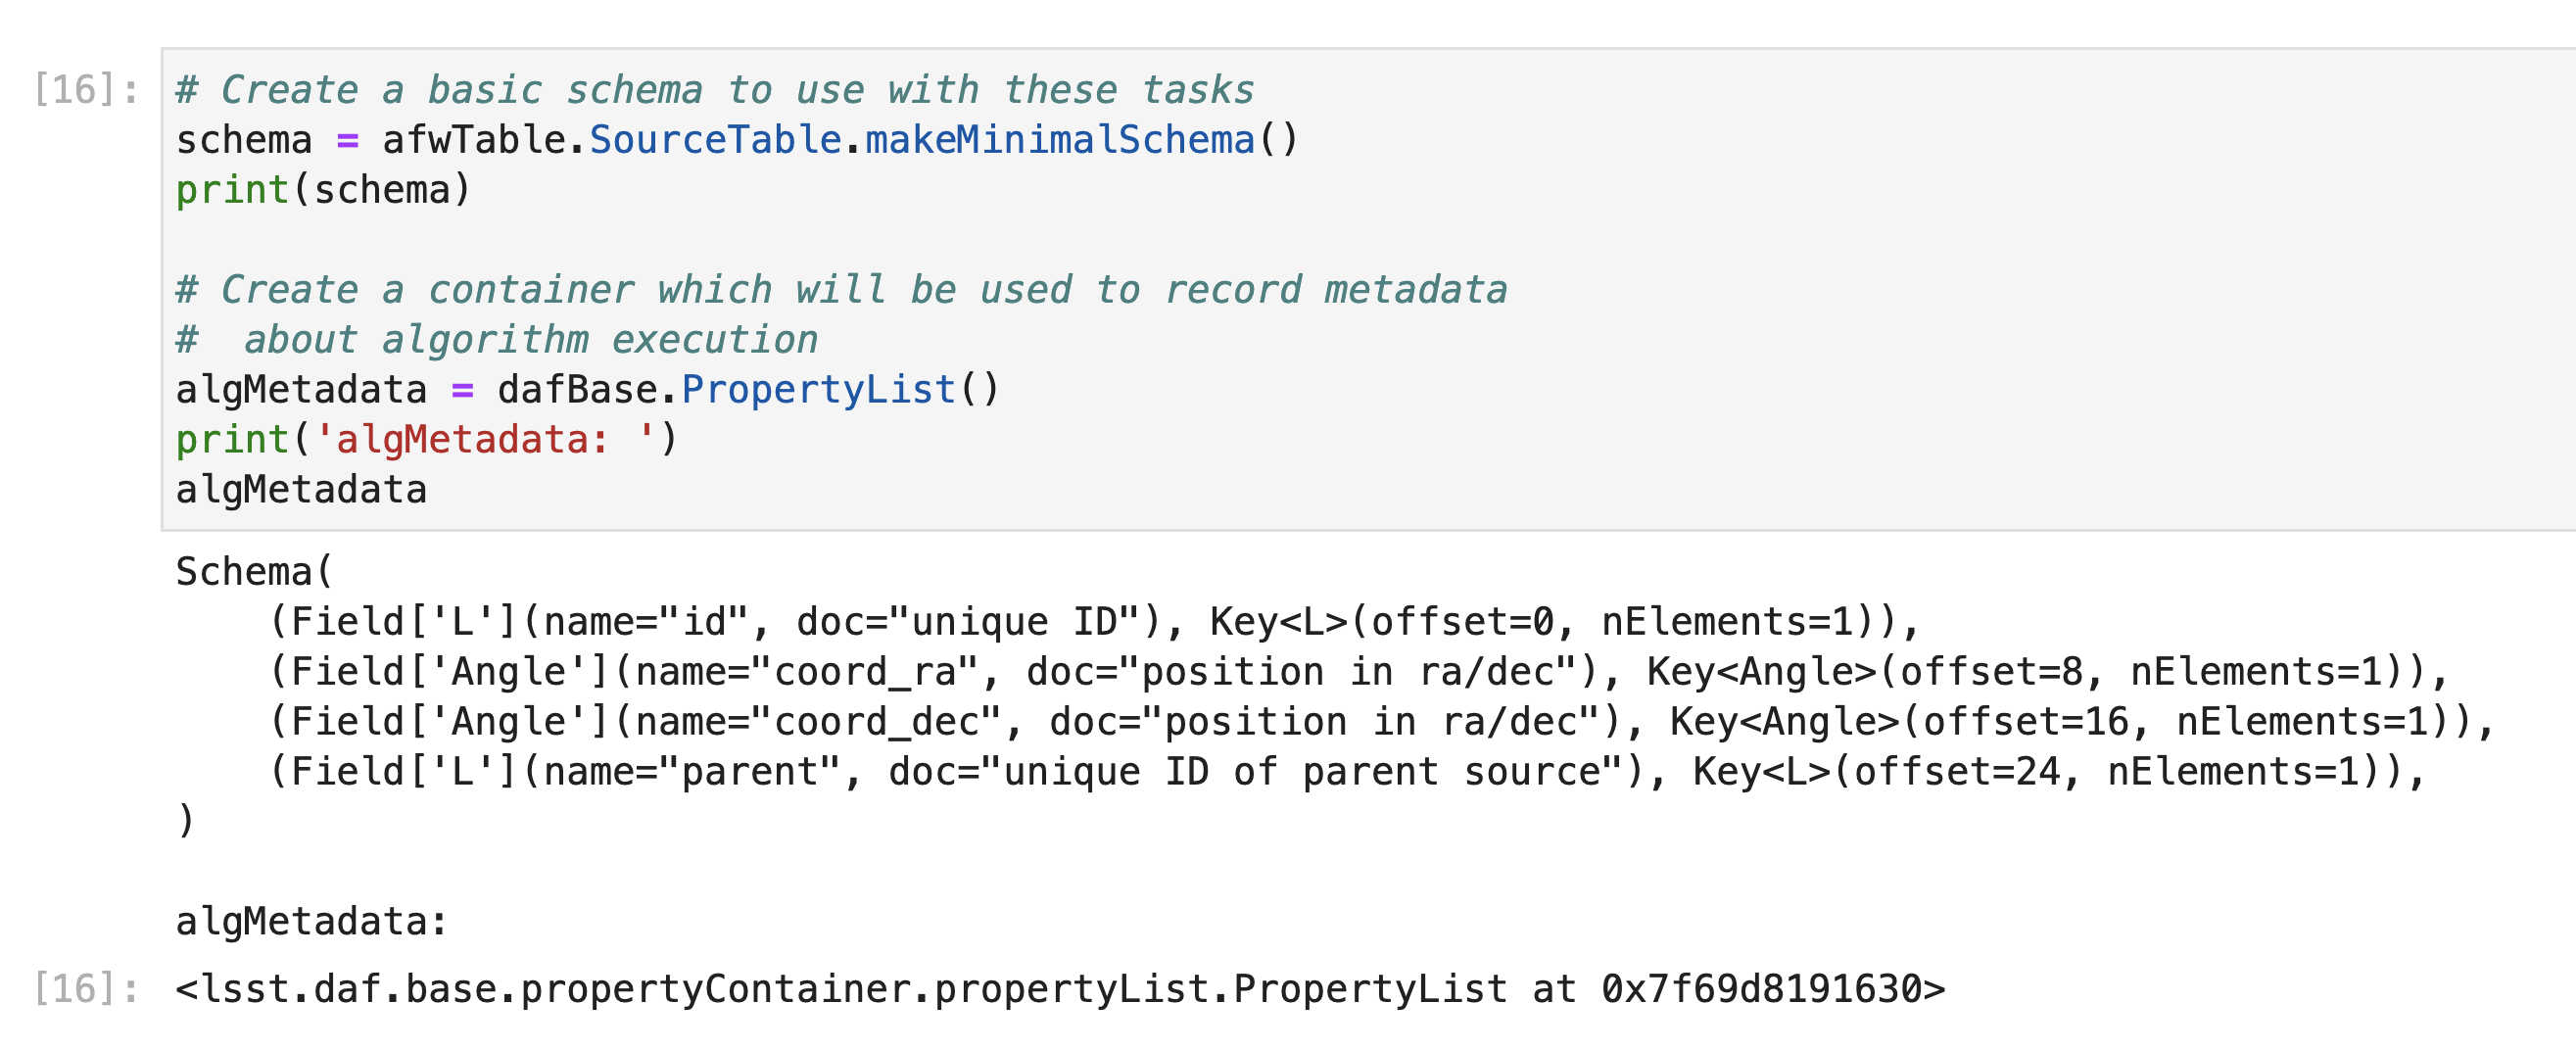
\includegraphics[width=5.97917in]{jira_imgs/2355.png}\\
After executing some other tasks, the notebook initialized the
configuration for `SourceDetectionTask` and changes some configuration
values:\\
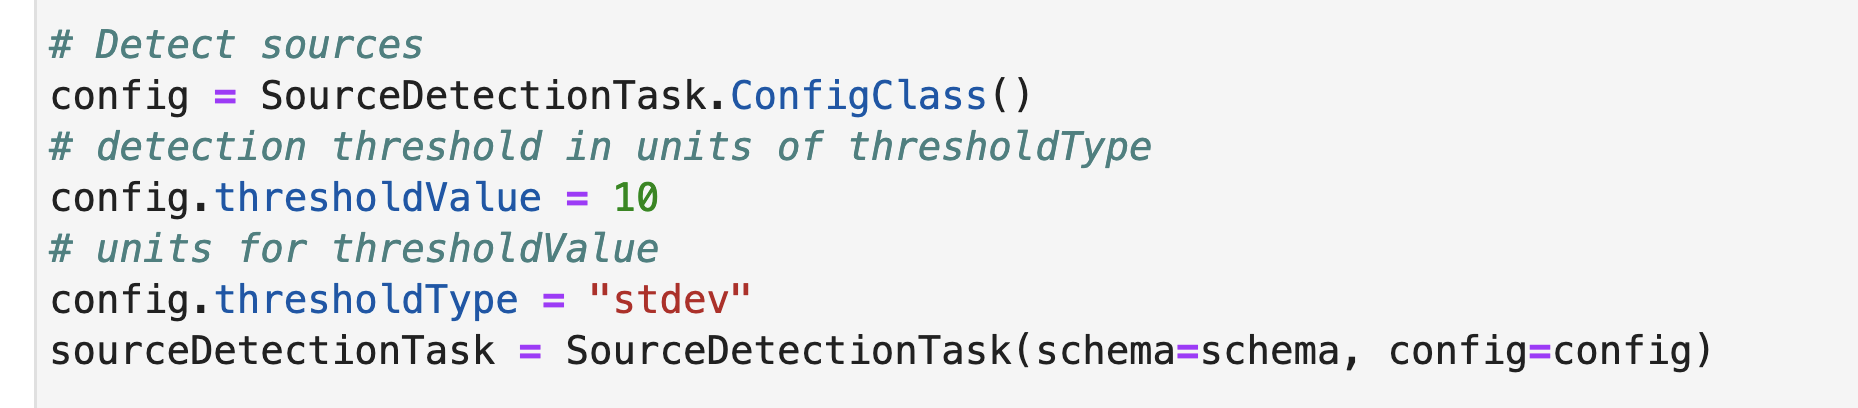
\includegraphics[width=6.02083in]{jira_imgs/2356.png}\\
Finally, the .run method of `SourceDetectionTask` is executed on an
input `calexp`, and returns a Struct containing the source table and
related objects:\\
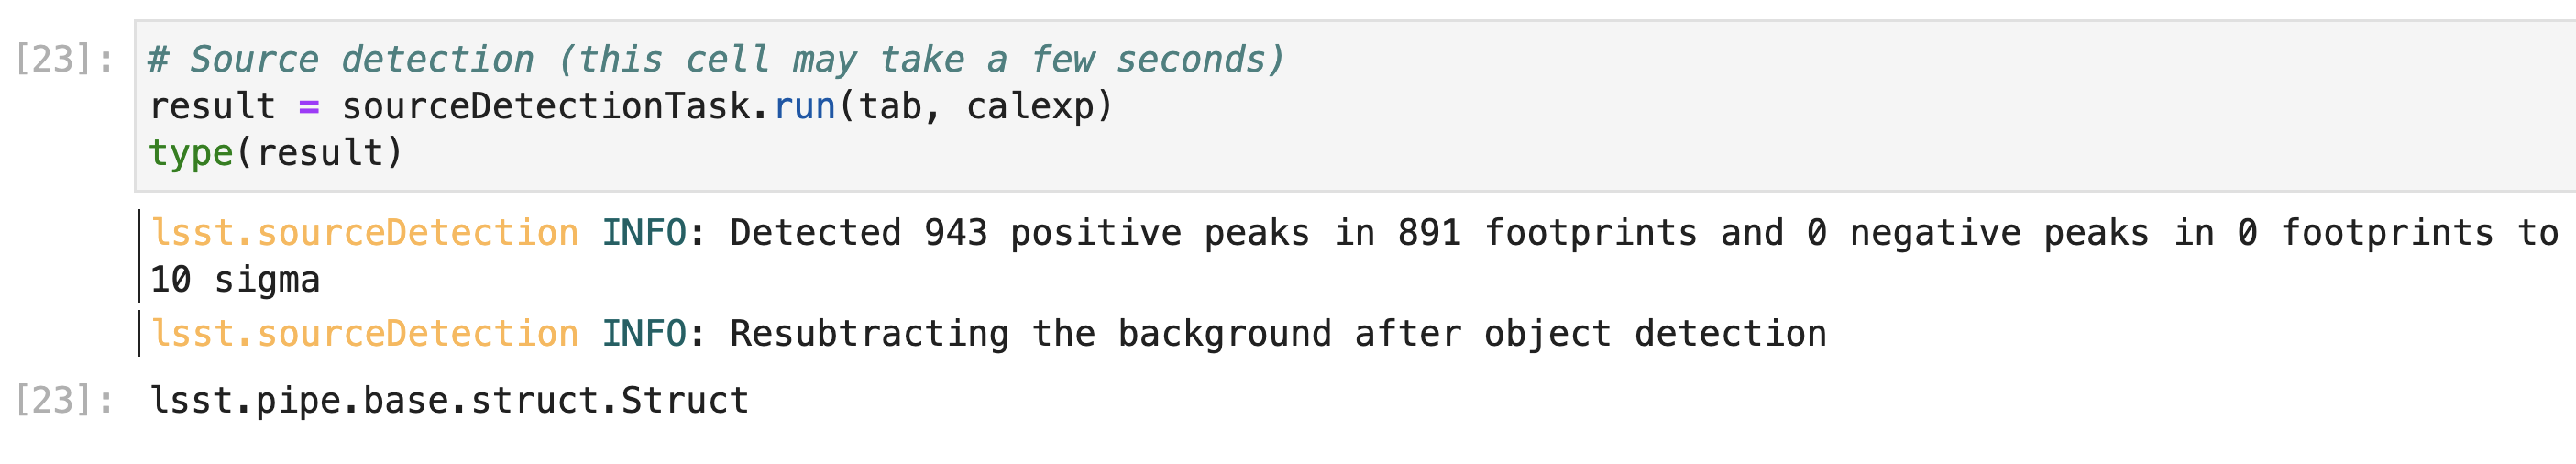
\includegraphics[width=6.06250in]{jira_imgs/2357.png}\\
We have thus demonstrated that the Pipeline interface can be accessed
via Python API.

}

\paragraph{ LVV-T2454 - Verify pre-execution config overrides }\mbox{}\\

Version \textbf{1}.
Open  \href{https://jira.lsstcorp.org/secure/Tests.jspa#/testCase/LVV-T2454}{\textit{ LVV-T2454 } }
test case in Jira.

Verify that the middleware enables programmatic overrides to the
configurations specified for a Pipeline, and that the overrides can be
captured for purposes of provenance recording.

\textbf{ Preconditions}:\\


Execution status: {\bf Pass }

Final comment:\\


Detailed steps results:

\begin{tabular}{p{2cm}p{14cm}}
\toprule
Step 1 & Step Execution Status: \textbf{ Pass } \\ \hline
\end{tabular}
 Description \\
{\footnotesize
Execute a set of pipeline tasks (e.g., ``step1'') on some data with
default config from DRP-RC2.yaml

}
\hdashrule[0.5ex]{\textwidth}{1pt}{3mm}
  Expected Result \\
{\footnotesize
Run results written to ``collection1''

}
\hdashrule[0.5ex]{\textwidth}{1pt}{3mm}
  Actual Result \\
{\footnotesize
Working on lsst-devl machines at NCSA, set up the Science Pipelines,
then set up the `rc2\_subset` repo.\\[2\baselineskip]Copy the
``default'' RC2 pipeline to the local directory:\\
cp \$DRP\_PIPE\_DIR/pipelines/HSC/DRP-RC2.yaml
./\\[2\baselineskip]Execute ``step1'' from this pipeline, choosing only
a single detector and two visits:\\
pipetask run -j 8 -b \$RC2\_SUBSET\_DIR/SMALL\_HSC/butler.yaml -p
DRP-RC2.yaml\#step1 -i HSC/RC2/defaults -o
u/jcarlin/pipetask\_config\_test1\_LDM556 -d ``detector in (42) AND
visit in (11690, 11698)''

}
\begin{tabular}{p{2cm}p{14cm}}
\toprule
Step 2 & Step Execution Status: \textbf{ Pass } \\ \hline
\end{tabular}
 Description \\
{\footnotesize
Change a configuration option (in a version saved as DRP-RC2\_v2.yaml),
then execute the same pipeline tasks as in step 1, writing to a
different output collection.

}
\hdashrule[0.5ex]{\textwidth}{1pt}{3mm}
  Expected Result \\
{\footnotesize
Run results written to ``collection2''

}
\hdashrule[0.5ex]{\textwidth}{1pt}{3mm}
  Actual Result \\
{\footnotesize
Copy the pipeline file to DRP-RC2\_v2.yaml and add the following lines
to change the detection threshold in
characterizeImageTask:\\[2\baselineskip]```\\
tasks:\\
\hspace*{0.333em} characterizeImage:\\
\hspace*{0.333em} ~ class:
lsst.pipe.tasks.characterizeImage.CharacterizeImageTask\\
\hspace*{0.333em} ~ config:\\
\hspace*{0.333em} ~ ~ detection.thresholdValue: 10.0\\
```\\[2\baselineskip]Execute this pipeline on the same data as in step
1, but with a different output collection:\\
pipetask run -j 8 -b \$RC2\_SUBSET\_DIR/SMALL\_HSC/butler.yaml -p
DRP-RC2\_v2.yaml\#step1 -i HSC/RC2/defaults -o
u/jcarlin/pipetask\_config\_test2\_LDM556 -d ``detector in (42) AND
visit in (11690, 11698)''

}
\begin{tabular}{p{2cm}p{14cm}}
\toprule
Step 3 & Step Execution Status: \textbf{ Pass } \\ \hline
\end{tabular}
 Description \\
{\footnotesize
Retrieve resulting datasets and configurations using the butler and
confirm that the configuration change is persisted, and that it has
altered the results from processing.

}
\hdashrule[0.5ex]{\textwidth}{1pt}{3mm}
  Expected Result \\
{\footnotesize
Configurations persisted in collection1 and collection2 differ, and the
results of processing also differ between the two runs.

}
\hdashrule[0.5ex]{\textwidth}{1pt}{3mm}
  Actual Result \\
{\footnotesize
In LVV-T2454.py:\\[2\baselineskip]from lsst.daf.butler import
Butler\\[2\baselineskip]\# Initialize the butler separately with each
collection:\\
butler=Butler('/project/jcarlin/repos/rc2\_subset/SMALL\_HSC/',
collections={[}'u/jcarlin/pipetask\_config\_test1\_LDM556'{]})\\
butler2=Butler('/project/jcarlin/repos/rc2\_subset/SMALL\_HSC/',
collections={[}'u/jcarlin/pipetask\_config\_test2\_LDM556'{]})\\[2\baselineskip]\#
Pick a single visit/detector:\\
dataId1 = \{'visit':11690, `detector':42,
`instrument':'HSC'\}\\[2\baselineskip]\# Extract the source tables for
the two runs:\\
src1 = butler.get('src', dataId1)\\
src2 = butler2.get('src', dataId1)\\[2\baselineskip]\# Print the length
of the source tables:\\
print('src1 length: ', len(src1))\\
print('src2 length: ', len(src2))\\[2\baselineskip]\# Extract the
configs for each run\\
cfg1 = butler.get('characterizeImage\_config', dataId1).toDict()\\
cfg2 = butler2.get('characterizeImage\_config',
dataId1).toDict()\\[2\baselineskip]\# Print the
detection.thresholdValue, since that's what we changed between the two
configs:\\
print('run1 threshold: `, cfg1{[}'detection'{]}{[}'thresholdValue'{]})\\
print('run2 threshold: `,
cfg2{[}'detection'{]}{[}'thresholdValue'{]})\\[2\baselineskip]Executing
this prints the following to the screen:\\
python LVV-T2454.py\\[2\baselineskip]src1 length: 3447\\
src2 length: 3369\\
run1 threshold: 5.0\\
run2 threshold: 10.0\\[2\baselineskip]We have demonstrated that the
configuration options can be overridden in specification, and that these
are persisted in the output repository.

}

\paragraph{ LVV-T2458 - Verify serialization of pre-flight results }\mbox{}\\

Version \textbf{1}.
Open  \href{https://jira.lsstcorp.org/secure/Tests.jspa#/testCase/LVV-T2458}{\textit{ LVV-T2458 } }
test case in Jira.

Verify that the supervisory framework provides a serialization form for
the results of the ``Pre-flight'' phase, so that they can be computed in
one process and executed under the control of one or more others.

\textbf{ Preconditions}:\\


Execution status: {\bf Pass }

Final comment:\\


Detailed steps results:

\begin{tabular}{p{2cm}p{14cm}}
\toprule
Step 1 & Step Execution Status: \textbf{ Pass } \\ \hline
\end{tabular}
 Description \\
{\footnotesize
Satisfied by QuantumGraph being serializable. Demonstrate using unit
tests in https://github.com/lsst/pipe\_base/tests/test\_quantumGraph.py

}
\hdashrule[0.5ex]{\textwidth}{1pt}{3mm}
  Expected Result \\
{\footnotesize
Unit test passes.

}
\hdashrule[0.5ex]{\textwidth}{1pt}{3mm}
  Actual Result \\
{\footnotesize
On lsst-devl machines at NCSA, working in a cloned `pipe\_base`
repository at
/project/jcarlin/SVV/gen3\_middleware\_acceptance\_testing/pipe\_base.\\[2\baselineskip]Execute
the unit tests that thoroughly tests quantum graph generation and
usage:\\
pytest -s -vv --no-header --cache-clear tests/test\_quantumGraph.py
\textbar{} tee
test\_QG\_log.txt\\[2\baselineskip]tests/test\_quantumGraph.py::FLAKE8
PASSED\\
tests/test\_quantumGraph.py::QuantumGraphTestCase::testAllDatasetTypes
PASSED\\
tests/test\_quantumGraph.py::QuantumGraphTestCase::testContains PASSED\\
tests/test\_quantumGraph.py::QuantumGraphTestCase::testDetermineAnsestorsOfQuantumNode
PASSED\\
tests/test\_quantumGraph.py::QuantumGraphTestCase::testDetermineConnectionsOfQuantum
PASSED\\
tests/test\_quantumGraph.py::QuantumGraphTestCase::testDetermineOutputsOfQuantumNode
PASSED\\
tests/test\_quantumGraph.py::QuantumGraphTestCase::testFindCycle
PASSED\\
tests/test\_quantumGraph.py::QuantumGraphTestCase::testFindQuantaWIthDSType
PASSED\\
tests/test\_quantumGraph.py::QuantumGraphTestCase::testFindTaskDefByLabel
PASSED\\
tests/test\_quantumGraph.py::QuantumGraphTestCase::testFindTaskDefByName
PASSED\\
tests/test\_quantumGraph.py::QuantumGraphTestCase::testFindTasksWithInput
PASSED\\
tests/test\_quantumGraph.py::QuantumGraphTestCase::testFindTasksWithOutput
PASSED\\
tests/test\_quantumGraph.py::QuantumGraphTestCase::testGetNodesForTask
PASSED\\
tests/test\_quantumGraph.py::QuantumGraphTestCase::testGetQuantaForTask
PASSED\\
tests/test\_quantumGraph.py::QuantumGraphTestCase::testGetQuantumNodeByNodeId
PASSED\\
tests/test\_quantumGraph.py::QuantumGraphTestCase::testGraph PASSED\\
tests/test\_quantumGraph.py::QuantumGraphTestCase::testInputQuanta
PASSED\\
tests/test\_quantumGraph.py::QuantumGraphTestCase::testLength PASSED\\
tests/test\_quantumGraph.py::QuantumGraphTestCase::testOutputtQuanta
PASSED\\
tests/test\_quantumGraph.py::QuantumGraphTestCase::testPickle PASSED\\
tests/test\_quantumGraph.py::QuantumGraphTestCase::testSaveLoad PASSED\\
tests/test\_quantumGraph.py::QuantumGraphTestCase::testSaveLoadUri
PASSED\\
tests/test\_quantumGraph.py::QuantumGraphTestCase::testSaveLoadUriS3
PASSED\\
tests/test\_quantumGraph.py::QuantumGraphTestCase::testSubset PASSED\\
tests/test\_quantumGraph.py::QuantumGraphTestCase::testSubsetToConnected
PASSED\\
tests/test\_quantumGraph.py::QuantumGraphTestCase::testTaskGraph
PASSED\\
tests/test\_quantumGraph.py::QuantumGraphTestCase::testTaskWithDSType
PASSED\\
tests/test\_quantumGraph.py::MyMemoryTestCase::testFileDescriptorLeaks
\textless{}-
../../../../../software/lsstsw/stack\_20220215/stack/miniconda3-py38\_4.9.2-2.0.0/Linux64/utils/g617c0b0dc2+9633a190c8/python/lsst/utils/tests.py
PASSED\\[2\baselineskip]All passed. These tests (particularly the ones
with ``SaveLoad'' in their names)demonstrate that the quantum graphs can
be serialized and read in to initiate execution.\\[2\baselineskip]

}

\paragraph{ LVV-T2451 - Verify ability to append to an existing repository }\mbox{}\\

Version \textbf{1}.
Open  \href{https://jira.lsstcorp.org/secure/Tests.jspa#/testCase/LVV-T2451}{\textit{ LVV-T2451 } }
test case in Jira.

Verify that it is possible to add Datasets to a pre-existing Collection
via additional processing.

\textbf{ Preconditions}:\\


Execution status: {\bf Pass }

Final comment:\\


Detailed steps results:

\begin{tabular}{p{2cm}p{14cm}}
\toprule
Step 1 & Step Execution Status: \textbf{ Pass } \\ \hline
\end{tabular}
 Description \\
{\footnotesize
Execute unit tests in
\url{https://github.com/lsst/daf_butler/blob/main/tests/test_butler.py}
(in particular, ButlerPutGetTests demonstrate creating a collection,
then adding datasets to it.

}
\hdashrule[0.5ex]{\textwidth}{1pt}{3mm}
  Expected Result \\
{\footnotesize
Unit test passes

}
\hdashrule[0.5ex]{\textwidth}{1pt}{3mm}
  Actual Result \\
{\footnotesize
On lsst-devl machines at NCSA, in a cloned `daf\_butler` repository (at
/project/jcarlin/SVV/gen3\_middleware\_acceptance\_testing/daf\_butler),
execute:\\[2\baselineskip]pytest -s -vv --no-header --cache-clear
tests/test\_butler.py\\[2\baselineskip]Results:\\
tests/test\_butler.py::PosixDatastoreButlerTestCase::testBasicPutGet~PASSED\\
tests/test\_butler.py::PosixDatastoreButlerTestCase::testButlerRewriteDataId
PASSED\\
tests/test\_butler.py::PosixDatastoreButlerTestCase::testCompositePutGetConcrete
PASSED\\
tests/test\_butler.py::PosixDatastoreButlerTestCase::testCompositePutGetVirtual
PASSED\\
tests/test\_butler.py::InMemoryDatastoreButlerTestCase::testBasicPutGet~PASSED\\
tests/test\_butler.py::InMemoryDatastoreButlerTestCase::testButlerRewriteDataId
PASSED\\
tests/test\_butler.py::InMemoryDatastoreButlerTestCase::testCompositePutGetConcrete
PASSED\\
tests/test\_butler.py::InMemoryDatastoreButlerTestCase::testCompositePutGetVirtual
PASSED\\
tests/test\_butler.py::ChainedDatastoreButlerTestCase::testBasicPutGet~PASSED\\
tests/test\_butler.py::ChainedDatastoreButlerTestCase::testButlerRewriteDataId
PASSED\\
tests/test\_butler.py::ChainedDatastoreButlerTestCase::testCompositePutGetConcrete
PASSED\\
tests/test\_butler.py::ChainedDatastoreButlerTestCase::testCompositePutGetVirtual
PASSED\\
tests/test\_butler.py::ButlerExplicitRootTestCase::testBasicPutGet~PASSED\\
tests/test\_butler.py::ButlerExplicitRootTestCase::testButlerRewriteDataId
PASSED\\
tests/test\_butler.py::ButlerExplicitRootTestCase::testCompositePutGetConcrete
PASSED\\
tests/test\_butler.py::ButlerExplicitRootTestCase::testCompositePutGetVirtual
PASSED\\
tests/test\_butler.py::ButlerMakeRepoOutfileTestCase::testPutGet~PASSED\\
tests/test\_butler.py::ButlerMakeRepoOutfileDirTestCase::testConfigExistence
PASSED\\
tests/test\_butler.py::ButlerMakeRepoOutfileDirTestCase::testDeferredCollectionPassing
PASSED\\
tests/test\_butler.py::ButlerMakeRepoOutfileDirTestCase::testPutGet~PASSED\\
tests/test\_butler.py::ButlerMakeRepoOutfileUriTestCase::testConfigExistence
PASSED\\
tests/test\_butler.py::ButlerMakeRepoOutfileUriTestCase::testDeferredCollectionPassing
PASSED\\
tests/test\_butler.py::ButlerMakeRepoOutfileUriTestCase::testPutGet~PASSED\\
tests/test\_butler.py::S3DatastoreButlerTestCase::testBasicPutGet~PASSED\\
tests/test\_butler.py::S3DatastoreButlerTestCase::testButlerRewriteDataId
PASSED\\
tests/test\_butler.py::S3DatastoreButlerTestCase::testCompositePutGetConcrete
PASSED\\
tests/test\_butler.py::S3DatastoreButlerTestCase::testCompositePutGetVirtual
PASSED\\[2\baselineskip]All tests of the butler's ``Put'' and ``Get''
functionality passed. These tests first create a ``run'' collection,
then append datasets to that collection, and thus demonstrate the
required functionality.

}

\paragraph{ LVV-T2453 - Verify creation of DatasetRef upon butler.put }\mbox{}\\

Version \textbf{1}.
Open  \href{https://jira.lsstcorp.org/secure/Tests.jspa#/testCase/LVV-T2453}{\textit{ LVV-T2453 } }
test case in Jira.

Verify that upon writing a dataset, a DatasetRef is created to enable
getting the dataset in the future.

\textbf{ Preconditions}:\\


Execution status: {\bf Pass }

Final comment:\\


Detailed steps results:

\begin{tabular}{p{2cm}p{14cm}}
\toprule
Step 1 & Step Execution Status: \textbf{ Pass } \\ \hline
\end{tabular}
 Description \\
{\footnotesize
Execute ButlerPutGetTests
in~\url{https://github.com/lsst/daf_butler/blob/main/tests/test_butler.py}

}
\hdashrule[0.5ex]{\textwidth}{1pt}{3mm}
  Expected Result \\
{\footnotesize
Unit test passes

}
\hdashrule[0.5ex]{\textwidth}{1pt}{3mm}
  Actual Result \\
{\footnotesize
On lsst-devl machines at NCSA, in a cloned `daf\_butler` repository (at
/project/jcarlin/SVV/gen3\_middleware\_acceptance\_testing/daf\_butler),
execute:\\[2\baselineskip]pytest -s -vv --no-header --cache-clear
tests/test\_butler.py\\[2\baselineskip]Results:\\
tests/test\_butler.py::PosixDatastoreButlerTestCase::testBasicPutGet~PASSED\\
tests/test\_butler.py::PosixDatastoreButlerTestCase::testButlerRewriteDataId
PASSED\\
tests/test\_butler.py::PosixDatastoreButlerTestCase::testCompositePutGetConcrete
PASSED\\
tests/test\_butler.py::PosixDatastoreButlerTestCase::testCompositePutGetVirtual
PASSED\\
tests/test\_butler.py::InMemoryDatastoreButlerTestCase::testBasicPutGet~PASSED\\
tests/test\_butler.py::InMemoryDatastoreButlerTestCase::testButlerRewriteDataId
PASSED\\
tests/test\_butler.py::InMemoryDatastoreButlerTestCase::testCompositePutGetConcrete
PASSED\\
tests/test\_butler.py::InMemoryDatastoreButlerTestCase::testCompositePutGetVirtual
PASSED\\
tests/test\_butler.py::ChainedDatastoreButlerTestCase::testBasicPutGet~PASSED\\
tests/test\_butler.py::ChainedDatastoreButlerTestCase::testButlerRewriteDataId
PASSED\\
tests/test\_butler.py::ChainedDatastoreButlerTestCase::testCompositePutGetConcrete
PASSED\\
tests/test\_butler.py::ChainedDatastoreButlerTestCase::testCompositePutGetVirtual
PASSED\\
tests/test\_butler.py::ButlerExplicitRootTestCase::testBasicPutGet~PASSED\\
tests/test\_butler.py::ButlerExplicitRootTestCase::testButlerRewriteDataId
PASSED\\
tests/test\_butler.py::ButlerExplicitRootTestCase::testCompositePutGetConcrete
PASSED\\
tests/test\_butler.py::ButlerExplicitRootTestCase::testCompositePutGetVirtual
PASSED\\
tests/test\_butler.py::ButlerMakeRepoOutfileTestCase::testPutGet~PASSED\\
tests/test\_butler.py::ButlerMakeRepoOutfileDirTestCase::testConfigExistence
PASSED\\
tests/test\_butler.py::ButlerMakeRepoOutfileDirTestCase::testDeferredCollectionPassing
PASSED\\
tests/test\_butler.py::ButlerMakeRepoOutfileDirTestCase::testPutGet~PASSED\\
tests/test\_butler.py::ButlerMakeRepoOutfileUriTestCase::testConfigExistence
PASSED\\
tests/test\_butler.py::ButlerMakeRepoOutfileUriTestCase::testDeferredCollectionPassing
PASSED\\
tests/test\_butler.py::ButlerMakeRepoOutfileUriTestCase::testPutGet~PASSED\\
tests/test\_butler.py::S3DatastoreButlerTestCase::testBasicPutGet~PASSED\\
tests/test\_butler.py::S3DatastoreButlerTestCase::testButlerRewriteDataId
PASSED\\
tests/test\_butler.py::S3DatastoreButlerTestCase::testCompositePutGetConcrete
PASSED\\
tests/test\_butler.py::S3DatastoreButlerTestCase::testCompositePutGetVirtual
PASSED\\[2\baselineskip]All tests of the butler's ``Put'' and ``Get''
functionality passed.

}

\paragraph{ LVV-T2449 - Verify middleware writer configurability }\mbox{}\\

Version \textbf{1}.
Open  \href{https://jira.lsstcorp.org/secure/Tests.jspa#/testCase/LVV-T2449}{\textit{ LVV-T2449 } }
test case in Jira.

Verify that the data output system supports configuration of individual
writer behavior.

\textbf{ Preconditions}:\\


Execution status: {\bf Pass }

Final comment:\\


Detailed steps results:

\begin{tabular}{p{2cm}p{14cm}}
\toprule
Step 1 & Step Execution Status: \textbf{ Pass } \\ \hline
\end{tabular}
 Description \\
{\footnotesize
Execute the unit test at
\url{https://github.com/lsst/daf_butler/blob/main/tests/test_config.py},
which tests the writer configuration.

}
\hdashrule[0.5ex]{\textwidth}{1pt}{3mm}
  Expected Result \\
{\footnotesize
Unit test passes.

}
\hdashrule[0.5ex]{\textwidth}{1pt}{3mm}
  Actual Result \\
{\footnotesize
On lsst-devl machines at NCSA, in a cloned `daf\_butler` repository (at
/project/jcarlin/SVV/gen3\_middleware\_acceptance\_testing/daf\_butler),
execute:\\[2\baselineskip]pytest -s -vv --no-header --cache-clear
tests/test\_config.py\\[2\baselineskip]Results:\\[2\baselineskip]tests/test\_config.py::FLAKE8
PASSED\\
tests/test\_config.py::ConfigTestCase::testBadConfig~PASSED\\
tests/test\_config.py::ConfigTestCase::testBasics~PASSED\\
tests/test\_config.py::ConfigTestCase::testDict~PASSED\\
tests/test\_config.py::ConfigTestCase::testEscape~PASSED\\
tests/test\_config.py::ConfigTestCase::testHierarchy~PASSED\\
tests/test\_config.py::ConfigTestCase::testMerge~PASSED\\
tests/test\_config.py::ConfigTestCase::testOperators~PASSED\\
tests/test\_config.py::ConfigTestCase::testSerializedString~PASSED\\
tests/test\_config.py::ConfigTestCase::testSplitting~PASSED\\
tests/test\_config.py::ConfigTestCase::testUpdate~PASSED\\
tests/test\_config.py::ConfigSubsetTestCase::testAbsPath~PASSED\\
tests/test\_config.py::ConfigSubsetTestCase::testClassDerived~PASSED\\
tests/test\_config.py::ConfigSubsetTestCase::testDefaults~PASSED\\
tests/test\_config.py::ConfigSubsetTestCase::testEmpty~PASSED\\
tests/test\_config.py::ConfigSubsetTestCase::testExternalHierarchy~PASSED\\
tests/test\_config.py::ConfigSubsetTestCase::testExternalOverride~PASSED\\
tests/test\_config.py::ConfigSubsetTestCase::testInclude~PASSED\\
tests/test\_config.py::ConfigSubsetTestCase::testIncludeConfigs~PASSED\\
tests/test\_config.py::ConfigSubsetTestCase::testNoDefaults~PASSED\\
tests/test\_config.py::ConfigSubsetTestCase::testPathlib~PASSED\\
tests/test\_config.py::ConfigSubsetTestCase::testResource~PASSED\\
tests/test\_config.py::ConfigSubsetTestCase::testSearchPaths~PASSED\\
tests/test\_config.py::ConfigSubsetTestCase::testStringInclude~PASSED\\
tests/test\_config.py::FileWriteConfigTestCase::testDump
PASSED\\[2\baselineskip]This confirms that the writer behavior can be
configured.

}

\paragraph{ LVV-T2452 - Verify specification of output locations }\mbox{}\\

Version \textbf{1}.
Open  \href{https://jira.lsstcorp.org/secure/Tests.jspa#/testCase/LVV-T2452}{\textit{ LVV-T2452 } }
test case in Jira.

Verify that the middleware enables configuration of the output location
for a POSIX file system.

\textbf{ Preconditions}:\\


Execution status: {\bf Pass }

Final comment:\\Working with a cloned `daf\_butler` repository
at~/project/jcarlin/SVV/gen3\_middleware\_acceptance\_testing/daf\_butler
on the lsst-devl machines.


Detailed steps results:

\begin{tabular}{p{2cm}p{14cm}}
\toprule
Step 1 & Step Execution Status: \textbf{ Pass } \\ \hline
\end{tabular}
 Description \\
{\footnotesize
Execute the PosixDatastoreButlerTestCase in
\url{https://github.com/lsst/daf_butler/blob/main/tests/test_butler.py}

}
\hdashrule[0.5ex]{\textwidth}{1pt}{3mm}
  Expected Result \\
{\footnotesize
Unit test passes

}
\hdashrule[0.5ex]{\textwidth}{1pt}{3mm}
  Actual Result \\
{\footnotesize
Executed the unit test via: ``pytest -s -vv --no-header
tests/test\_butler.py''\\[2\baselineskip]Results:\\[2\baselineskip]tests/test\_butler.py::PosixDatastoreButlerTestCase::testBasicPutGet
PASSED\\
tests/test\_butler.py::PosixDatastoreButlerTestCase::testButlerRewriteDataId
PASSED\\
tests/test\_butler.py::PosixDatastoreButlerTestCase::testCompositePutGetConcrete
PASSED\\
tests/test\_butler.py::PosixDatastoreButlerTestCase::testCompositePutGetVirtual
PASSED\\
tests/test\_butler.py::PosixDatastoreButlerTestCase::testConstructor
PASSED\\
tests/test\_butler.py::PosixDatastoreButlerTestCase::testDeferredCollectionPassing
PASSED\\
tests/test\_butler.py::PosixDatastoreButlerTestCase::testExportTransferCopy
PASSED\\
tests/test\_butler.py::PosixDatastoreButlerTestCase::testGetDatasetTypes
PASSED\\
tests/test\_butler.py::PosixDatastoreButlerTestCase::testImportExport
Root:
file:///project/jcarlin/SVV/gen3\_middleware\_acceptance\_testing/daf\_butler/tests/tmpdke1g8no/\\
PASSED\\
tests/test\_butler.py::PosixDatastoreButlerTestCase::testImportExportVirtualComposite
Root:
file:///project/jcarlin/SVV/gen3\_middleware\_acceptance\_testing/daf\_butler/tests/tmpdd9i5by4/\\
XFAIL\\
tests/test\_butler.py::PosixDatastoreButlerTestCase::testIngest PASSED\\
tests/test\_butler.py::PosixDatastoreButlerTestCase::testMakeRepo
PASSED\\
tests/test\_butler.py::PosixDatastoreButlerTestCase::testPathConstructor
PASSED\\
tests/test\_butler.py::PosixDatastoreButlerTestCase::testPickle PASSED\\
tests/test\_butler.py::PosixDatastoreButlerTestCase::testPruneCollections
PASSED\\
tests/test\_butler.py::PosixDatastoreButlerTestCase::testPruneDatasets
PASSED\\
tests/test\_butler.py::PosixDatastoreButlerTestCase::testPutTemplates
PASSED\\
tests/test\_butler.py::PosixDatastoreButlerTestCase::testPytypeCoercion
PASSED\\
tests/test\_butler.py::PosixDatastoreButlerTestCase::testPytypePutCoercion
PASSED\\
tests/test\_butler.py::PosixDatastoreButlerTestCase::testRemoveRuns
PASSED\\
tests/test\_butler.py::PosixDatastoreButlerTestCase::testStringification
PASSED\\
tests/test\_butler.py::PosixDatastoreButlerTestCase::testTransaction
PASSED\\[2\baselineskip]All of the tests in PosixDatastoreButlerTestCase
have passed.

}

\paragraph{ LVV-T2450 - Verify writing dataset to multiple repositories }\mbox{}\\

Version \textbf{1}.
Open  \href{https://jira.lsstcorp.org/secure/Tests.jspa#/testCase/LVV-T2450}{\textit{ LVV-T2450 } }
test case in Jira.

Verify that the middleware enables writing of a single dataset to
multiple repositories, with a different output format used for each
repository.

\textbf{ Preconditions}:\\


Execution status: {\bf Pass }

Final comment:\\


Detailed steps results:

\begin{tabular}{p{2cm}p{14cm}}
\toprule
Step 1 & Step Execution Status: \textbf{ Pass } \\ \hline
\end{tabular}
 Description \\
{\footnotesize
Execute the unit tests in
https://github.com/lsst/daf\_butler/blob/main/tests/test\_datastore.py
-- specifically, those involving `ChainedDatastore`s demonstrate this
behavior.

}
\hdashrule[0.5ex]{\textwidth}{1pt}{3mm}
  Expected Result \\
{\footnotesize
Unit test passes

}
\hdashrule[0.5ex]{\textwidth}{1pt}{3mm}
  Actual Result \\
{\footnotesize
On lsst-devl machines at NCSA, in a cloned `daf\_butler` repository (at
/project/jcarlin/SVV/gen3\_middleware\_acceptance\_testing/daf\_butler),
execute:\\[2\baselineskip]pytest -s -vv --no-header --cache-clear
tests/test\_datastore.py\\[2\baselineskip]The output contains the
following:\\[2\baselineskip]tests/test\_datastore.py::ChainedDatastoreTestCase::testBasicTransaction
PASSED\\
tests/test\_datastore.py::ChainedDatastoreTestCase::testConfigRoot
PASSED\\
tests/test\_datastore.py::ChainedDatastoreTestCase::testConfigurationValidation
PASSED\\
tests/test\_datastore.py::ChainedDatastoreTestCase::testConstructor
PASSED\\
tests/test\_datastore.py::ChainedDatastoreTestCase::testDisassembly
PASSED\\
tests/test\_datastore.py::ChainedDatastoreTestCase::testExportImportRecords
PASSED\\
tests/test\_datastore.py::ChainedDatastoreTestCase::testForget PASSED\\
tests/test\_datastore.py::ChainedDatastoreTestCase::testIngestNoTransfer
PASSED\\
tests/test\_datastore.py::ChainedDatastoreTestCase::testIngestSymlinkOfSymlink
Trying mode symlink\\
Trying mode relsymlink\\
PASSED\\
tests/test\_datastore.py::ChainedDatastoreTestCase::testIngestTransfer
PASSED\\
tests/test\_datastore.py::ChainedDatastoreTestCase::testNestedTransaction
PASSED\\
tests/test\_datastore.py::ChainedDatastoreTestCase::testParameterValidation
PASSED\\
tests/test\_datastore.py::ChainedDatastoreTestCase::testRegistryCompositePutGet
Using storageClass: StructuredComposite\\
Writing component output with StructuredDataDictYaml\\
Writing component summary with StructuredDataDictYaml\\
Writing component data with StructuredDataListYaml\\
Using storageClass: StructuredCompositeTestA\\
Writing component output with StructuredDataDictJson\\
Writing component summary with StructuredDataDictJson\\
Writing component data with StructuredDataListJson\\
Using storageClass: StructuredCompositeTestB\\
Writing component output with StructuredDataDictJson\\
Writing component summary with StructuredDataDictPickle\\
Writing component data with StructuredDataListYaml\\
PASSED\\
tests/test\_datastore.py::ChainedDatastoreTestCase::testRemove PASSED\\
tests/test\_datastore.py::ChainedDatastoreTestCase::testTransfer
PASSED\\
tests/test\_datastore.py::ChainedDatastoreTestCase::testTrustGetRequest
PASSED\\
tests/test\_datastore.py::ChainedDatastoreMemoryTestCase::testBasicPutGet
Using storageClass: StructuredData\\
Using storageClass: StructuredDataJson\\
Using storageClass: StructuredDataPickle\\
PASSED\\
tests/test\_datastore.py::ChainedDatastoreMemoryTestCase::testBasicTransaction
PASSED\\
tests/test\_datastore.py::ChainedDatastoreMemoryTestCase::testConfigRoot
PASSED\\
tests/test\_datastore.py::ChainedDatastoreMemoryTestCase::testConfigurationValidation
PASSED\\
tests/test\_datastore.py::ChainedDatastoreMemoryTestCase::testConstructor
PASSED\\
tests/test\_datastore.py::ChainedDatastoreMemoryTestCase::testDisassembly
PASSED\\
tests/test\_datastore.py::ChainedDatastoreMemoryTestCase::testExportImportRecords
SKIPPED\\
tests/test\_datastore.py::ChainedDatastoreMemoryTestCase::testForget
PASSED\\
tests/test\_datastore.py::ChainedDatastoreMemoryTestCase::testIngestNoTransfer
PASSED\\
tests/test\_datastore.py::ChainedDatastoreMemoryTestCase::testIngestSymlinkOfSymlink
PASSED\\
tests/test\_datastore.py::ChainedDatastoreMemoryTestCase::testIngestTransfer
PASSED\\
tests/test\_datastore.py::ChainedDatastoreMemoryTestCase::testNestedTransaction
PASSED\\
tests/test\_datastore.py::ChainedDatastoreMemoryTestCase::testParameterValidation
PASSED\\
tests/test\_datastore.py::ChainedDatastoreMemoryTestCase::testRegistryCompositePutGet
Using storageClass: StructuredComposite\\
tests/test\_datastore.py::ChainedDatastoreMemoryTestCase::testRemove
PASSED\\
tests/test\_datastore.py::ChainedDatastoreMemoryTestCase::testTransfer
PASSED\\
tests/test\_datastore.py::ChainedDatastoreMemoryTestCase::testTrustGetRequest
PASSED\\
tests/test\_datastore.py::PosixDatastoreConstraintsTestCase::testConstraints
PASSED\\
tests/test\_datastore.py::InMemoryDatastoreConstraintsTestCase::testConstraints
PASSED\\
tests/test\_datastore.py::ChainedDatastoreConstraintsNativeTestCase::testConstraints
PASSED\\
tests/test\_datastore.py::ChainedDatastoreConstraintsTestCase::testConstraints
PASSED\\
tests/test\_datastore.py::ChainedDatastoreMemoryConstraintsTestCase::testConstraints
PASSED\\
tests/test\_datastore.py::ChainedDatastorePerStoreConstraintsTests::testConstraints
PASSED\\
tests/test\_datastore.py::DatastoreCacheTestCase::testCacheExpiryAge
PASSED\\
tests/test\_datastore.py::DatastoreCacheTestCase::testCacheExpiryDatasets
PASSED\\
tests/test\_datastore.py::DatastoreCacheTestCase::testCacheExpiryDatasetsComposite
PASSED\\
tests/test\_datastore.py::DatastoreCacheTestCase::testCacheExpiryFiles
PASSED\\
tests/test\_datastore.py::DatastoreCacheTestCase::testCacheExpirySize
PASSED\\
tests/test\_datastore.py::DatastoreCacheTestCase::testExplicitCacheDir
PASSED\\
tests/test\_datastore.py::DatastoreCacheTestCase::testNoCache PASSED\\
tests/test\_datastore.py::DatastoreCacheTestCase::testNoCacheDir
PASSED\\
tests/test\_datastore.py::DatastoreCacheTestCase::testNoCacheDirReversed
PASSED\\[2\baselineskip]We have thus demonstrated that the middleware
enables writing a single dataset to multiple repositories with different
output formats.

}

\paragraph{ LVV-T2447 - Verify DataRepository layering: Data Release and Science Platform }\mbox{}\\

Version \textbf{1}.
Open  \href{https://jira.lsstcorp.org/secure/Tests.jspa#/testCase/LVV-T2447}{\textit{ LVV-T2447 } }
test case in Jira.

Verify that a Data Release is usable as the inputs for processing
initiated in the Science Platform.

\textbf{ Preconditions}:\\


Execution status: {\bf Not Executed }

Final comment:\\


Detailed steps results:

\begin{tabular}{p{2cm}p{14cm}}
\toprule
Step 1 & Step Execution Status: \textbf{ Not Executed } \\ \hline
\end{tabular}
 Description \\
{\footnotesize
Reuse test scirpt for DMS-MWBT-REQ-0012

}
\hdashrule[0.5ex]{\textwidth}{1pt}{3mm}
  Expected Result \\
{\footnotesize

}
\hdashrule[0.5ex]{\textwidth}{1pt}{3mm}
  Actual Result \\
{\footnotesize

}
\begin{tabular}{p{2cm}p{14cm}}
\toprule
Step 2 & Step Execution Status: \textbf{ Not Executed } \\ \hline
\end{tabular}
 Description \\
{\footnotesize
Run a DRP pipeline subset in RSP, using DP0.x collections as inputs.

}
\hdashrule[0.5ex]{\textwidth}{1pt}{3mm}
  Expected Result \\
{\footnotesize

}
\hdashrule[0.5ex]{\textwidth}{1pt}{3mm}
  Actual Result \\
{\footnotesize

}

\paragraph{ LVV-T2446 - Verify registries of collections }\mbox{}\\

Version \textbf{1}.
Open  \href{https://jira.lsstcorp.org/secure/Tests.jspa#/testCase/LVV-T2446}{\textit{ LVV-T2446 } }
test case in Jira.

Verify that there is a ~mechanism for registering Collections as they
are created

\textbf{ Preconditions}:\\


Execution status: {\bf Pass }

Final comment:\\


Detailed steps results:

\begin{tabular}{p{2cm}p{14cm}}
\toprule
Step 1 & Step Execution Status: \textbf{ Pass } \\ \hline
\end{tabular}
 Description \\
{\footnotesize
Execute `butler query-collections` to show that collections are
registered and searchable.

}
\hdashrule[0.5ex]{\textwidth}{1pt}{3mm}
  Expected Result \\
{\footnotesize

}
\hdashrule[0.5ex]{\textwidth}{1pt}{3mm}
  Actual Result \\
{\footnotesize
On lsst-devl machines at NCSA, set up the Science Pipelines, then
run:\\[2\baselineskip]butler query-collections /repo/main
*DM-341*\\[2\baselineskip]The glob ``*DM-341*'' should locate any
collection with that string in its name or path. (This is an arbitrarily
chosen string that should find collections related to Jira tickets with
ticket numbers DM-341??.)\\[2\baselineskip]Here is a portion of the
output from this query:\\[2\baselineskip]Name Type\\
------------------------------------------------------- -----------\\
HSC/runs/RC2/w\_2022\_12/DM-34125 CHAINED\\
HSC/runs/RC2/w\_2022\_12/DM-34125/20220324T205113Z RUN\\
HSC/runs/RC2/w\_2022\_12/DM-34125/20220321T222013Z RUN\\
HSC/runs/RC2/w\_2022\_12/DM-34125/20220325T213046Z RUN\\
HSC/runs/RC2/w\_2022\_12/DM-34125/20220325T211319Z RUN\\
HSC/runs/RC2/w\_2022\_12/DM-34125/20220323T173939Z RUN\\
HSC/runs/RC2/w\_2022\_12/DM-34125/20220321T153517Z RUN\\
HSC/runs/RC2/w\_2022\_12/DM-34125/20220319T213338Z RUN\\
HSC/raw/RC2/9615 TAGGED\\
HSC/raw/RC2/9697 TAGGED\\
HSC/raw/RC2/9813 TAGGED\\
HSC/calib/DM-32378 CALIBRATION\\
HSC/calib/gen2/20180117 CALIBRATION\\
HSC/calib/DM-28636 CALIBRATION\\
HSC/calib/gen2/20180117/unbounded RUN\\
HSC/calib/DM-28636/unbounded RUN\\
HSC/masks/s18a RUN\\
HSC/fgcmcal/lut/RC2/DM-28636 RUN\\
refcats/DM-28636 RUN\\
skymaps RUN\\
refcats/DM-33444 RUN\\
HSC/runs/RC2/w\_2022\_12/DM-34125/20220319T213338Z RUN\\
HSC/runs/RC2/w\_2022\_12/DM-34125/20220321T153517Z RUN\\
HSC/runs/RC2/w\_2022\_12/DM-34125/20220321T222013Z RUN\\
HSC/runs/RC2/w\_2022\_12/DM-34125/20220323T173939Z RUN\\
HSC/runs/RC2/w\_2022\_12/DM-34125/20220324T205113Z RUN\\
HSC/runs/RC2/w\_2022\_12/DM-34125/20220325T211319Z RUN\\
HSC/runs/RC2/w\_2022\_12/DM-34125/20220325T213046Z RUN\\
u/yusra/RC2/w\_2022\_12/DM-34125 CHAINED\\
u/yusra/RC2/w\_2022\_12/DM-34125/20220404T154651Z RUN\\
HSC/runs/RC2/w\_2022\_12/DM-34125/20220325T213046Z RUN\\
HSC/runs/RC2/w\_2022\_12/DM-34125/20220325T211319Z RUN\\
HSC/runs/RC2/w\_2022\_12/DM-34125/20220324T205113Z RUN\\
HSC/runs/RC2/w\_2022\_12/DM-34125/20220323T173939Z RUN\\
HSC/runs/RC2/w\_2022\_12/DM-34125/20220321T222013Z RUN\\
HSC/runs/RC2/w\_2022\_12/DM-34125/20220321T153517Z RUN\\
HSC/runs/RC2/w\_2022\_12/DM-34125/20220319T213338Z RUN\\
HSC/raw/RC2/9615 TAGGED\\
HSC/raw/RC2/9697 TAGGED\\
HSC/raw/RC2/9813 TAGGED\\
HSC/calib/DM-32378 CALIBRATION\\
HSC/calib/gen2/20180117 CALIBRATION\\
HSC/calib/DM-28636 CALIBRATION\\[2\baselineskip]We have thus
demonstrated that Collections are registered in butler
databases.\\[2\baselineskip]

}

\paragraph{ LVV-T2444 - Verify dataset garbage collection }\mbox{}\\

Version \textbf{1}.
Open  \href{https://jira.lsstcorp.org/secure/Tests.jspa#/testCase/LVV-T2444}{\textit{ LVV-T2444 } }
test case in Jira.

Verify that when a DataRepository is removed, the Datasets it references
are removed if and only if they are not also referenced by one or more
additional DataRepositories that have been explicitly
identified.\\[2\baselineskip]Note that the requirement text assumed a
slightly different collections model from what we have.~ ~ ~Instead of
``reference counting'' datasets, we have RUN collections that own
datasets and TAGGED collections that don't, but we still guard against
improper deletions as the requirement demands.

\textbf{ Preconditions}:\\


Execution status: {\bf Pass }

Final comment:\\


Detailed steps results:

\begin{tabular}{p{2cm}p{14cm}}
\toprule
Step 1 & Step Execution Status: \textbf{ Pass } \\ \hline
\end{tabular}
 Description \\
{\footnotesize
Make example repo, one each, ~POSIX and S3

}
\hdashrule[0.5ex]{\textwidth}{1pt}{3mm}
  Expected Result \\
{\footnotesize

}
\hdashrule[0.5ex]{\textwidth}{1pt}{3mm}
  Actual Result \\
{\footnotesize

}
\begin{tabular}{p{2cm}p{14cm}}
\toprule
Step 2 & Step Execution Status: \textbf{ Pass } \\ \hline
\end{tabular}
 Description \\
{\footnotesize
Create TAGGED collection and add some datasets to it.

}
\hdashrule[0.5ex]{\textwidth}{1pt}{3mm}
  Expected Result \\
{\footnotesize

}
\hdashrule[0.5ex]{\textwidth}{1pt}{3mm}
  Actual Result \\
{\footnotesize

}
\begin{tabular}{p{2cm}p{14cm}}
\toprule
Step 3 & Step Execution Status: \textbf{ Pass } \\ \hline
\end{tabular}
 Description \\
{\footnotesize
Try to delete the RUN collection - shouldn't be possible because of
references in TAGGED collection.

}
\hdashrule[0.5ex]{\textwidth}{1pt}{3mm}
  Expected Result \\
{\footnotesize

}
\hdashrule[0.5ex]{\textwidth}{1pt}{3mm}
  Actual Result \\
{\footnotesize

}
\begin{tabular}{p{2cm}p{14cm}}
\toprule
Step 4 & Step Execution Status: \textbf{ Pass } \\ \hline
\end{tabular}
 Description \\
{\footnotesize
Try to delete the TAGGED collection - should work, without deleting the
datasets.

}
\hdashrule[0.5ex]{\textwidth}{1pt}{3mm}
  Expected Result \\
{\footnotesize

}
\hdashrule[0.5ex]{\textwidth}{1pt}{3mm}
  Actual Result \\
{\footnotesize
All of the steps suggested in this test script are executed in the
test\_cliCmdPruneCollection.py unit test from daf\_butler. Execute
this:\\[2\baselineskip]pytest -s -vv --no-header --cache-clear
tests/test\_cliCmdPruneCollection.py\\[2\baselineskip]tests/test\_cliCmdPruneCollection.py::PruneCollectionsTest::testPruneCollections
PASSED\\
tests/test\_cliCmdPruneCollection.py::PruneCollectionExecutionTest::testPruneRun~PASSED\\
tests/test\_cliCmdPruneCollection.py::PruneCollectionExecutionTest::testPruneTagged
PASSED\\[2\baselineskip]The unit test includes verification that a
TAGGED collection can be removed, and that RUN collections cannot be
removed without purging and unstoring the datasets.

}

\paragraph{ LVV-T2442 - Verify dataset deletion }\mbox{}\\

Version \textbf{1}.
Open  \href{https://jira.lsstcorp.org/secure/Tests.jspa#/testCase/LVV-T2442}{\textit{ LVV-T2442 } }
test case in Jira.

Verify that a Dataset is deletable from a DataRepository by an
authorized person.

\textbf{ Preconditions}:\\


Execution status: {\bf Initial Pass }

Final comment:\\


Detailed steps results:

\begin{tabular}{p{2cm}p{14cm}}
\toprule
Step 1 & Step Execution Status: \textbf{ Initial Pass } \\ \hline
\end{tabular}
 Description \\
{\footnotesize
Make example repo, one each,~ POSIX and S3

}
\hdashrule[0.5ex]{\textwidth}{1pt}{3mm}
  Expected Result \\
{\footnotesize

}
\hdashrule[0.5ex]{\textwidth}{1pt}{3mm}
  Actual Result \\
{\footnotesize

}
\begin{tabular}{p{2cm}p{14cm}}
\toprule
Step 2 & Step Execution Status: \textbf{ Pass } \\ \hline
\end{tabular}
 Description \\
{\footnotesize
Run `butler prune-datasets`

}
\hdashrule[0.5ex]{\textwidth}{1pt}{3mm}
  Expected Result \\
{\footnotesize

}
\hdashrule[0.5ex]{\textwidth}{1pt}{3mm}
  Actual Result \\
{\footnotesize
On lsst-devl machines at NCSA, in a cloned `daf\_butler` repository (at
/project/jcarlin/SVV/gen3\_middleware\_acceptance\_testing/daf\_butler),
execute:\\[2\baselineskip]pytest -s -vv --no-header --cache-clear
tests/test\_cliCmdPruneDatasets.py\\[2\baselineskip]The results show
that the deletion of datasets was
successful:\\[2\baselineskip]tests/test\_cliCmdPruneDatasets.py::FLAKE8~PASSED\\
tests/test\_cliCmdPruneDatasets.py::PruneDatasetsTestCase::test\_defaults\_doContinue~PASSED\\
tests/test\_cliCmdPruneDatasets.py::PruneDatasetsTestCase::test\_defaults\_doNotContinue~PASSED\\
tests/test\_cliCmdPruneDatasets.py::PruneDatasetsTestCase::test\_disassociateImpliedArgs~PASSED\\
tests/test\_cliCmdPruneDatasets.py::PruneDatasetsTestCase::test\_disassociateImpliedArgsWithCollections~PASSED\\
tests/test\_cliCmdPruneDatasets.py::PruneDatasetsTestCase::test\_dryRun\_disassociate~PASSED\\
tests/test\_cliCmdPruneDatasets.py::PruneDatasetsTestCase::test\_dryRun\_unstore~PASSED\\
tests/test\_cliCmdPruneDatasets.py::PruneDatasetsTestCase::test\_dryRun\_unstoreAndDisassociate~PASSED\\
tests/test\_cliCmdPruneDatasets.py::PruneDatasetsTestCase::test\_noCollections~PASSED\\
tests/test\_cliCmdPruneDatasets.py::PruneDatasetsTestCase::test\_noConfirm~PASSED\\
tests/test\_cliCmdPruneDatasets.py::PruneDatasetsTestCase::test\_noDatasets~PASSED\\
tests/test\_cliCmdPruneDatasets.py::PruneDatasetsTestCase::test\_purgeImpliedArgs~PASSED\\
tests/test\_cliCmdPruneDatasets.py::PruneDatasetsTestCase::test\_purgeImpliedArgsWithCollections~PASSED\\
tests/test\_cliCmdPruneDatasets.py::PruneDatasetsTestCase::test\_purgeOnNonRunCollection~PASSED\\
tests/test\_cliCmdPruneDatasets.py::PruneDatasetsTestCase::test\_purgeWithDisassociate~PASSED\\
tests/test\_cliCmdPruneDatasets.py::PruneDatasetsTestCase::test\_quiet~PASSED\\
tests/test\_cliCmdPruneDatasets.py::PruneDatasetsTestCase::test\_quietWithDryRun~PASSED\\[2\baselineskip]

}
\begin{tabular}{p{2cm}p{14cm}}
\toprule
Step 3 & Step Execution Status: \textbf{ Pass } \\ \hline
\end{tabular}
 Description \\
{\footnotesize
Verify that the datasets are deleted

}
\hdashrule[0.5ex]{\textwidth}{1pt}{3mm}
  Expected Result \\
{\footnotesize

}
\hdashrule[0.5ex]{\textwidth}{1pt}{3mm}
  Actual Result \\
{\footnotesize
The unit test includes steps that confirm the deletion of the datasets.~

}

\paragraph{ LVV-T2443 - Verify repository removal }\mbox{}\\

Version \textbf{1}.
Open  \href{https://jira.lsstcorp.org/secure/Tests.jspa#/testCase/LVV-T2443}{\textit{ LVV-T2443 } }
test case in Jira.

Verify that an authorized user can remove a DataRepository from any
storage environment. Verification on \textbf{all} environments is not
possible. We will verify POSIX and S3 environments, which we believe is
in the spirit of the requirement and covers our core needs.

\textbf{ Preconditions}:\\


Execution status: {\bf Initial Pass }

Final comment:\\


Detailed steps results:

\begin{tabular}{p{2cm}p{14cm}}
\toprule
Step 1 & Step Execution Status: \textbf{ Initial Pass } \\ \hline
\end{tabular}
 Description \\
{\footnotesize
Make example repo, one each, ~POSIX and S3

}
\hdashrule[0.5ex]{\textwidth}{1pt}{3mm}
  Expected Result \\
{\footnotesize

}
\hdashrule[0.5ex]{\textwidth}{1pt}{3mm}
  Actual Result \\
{\footnotesize
Tested on a POSIX datastore at NCSA (lsst-devl machines).

}
\begin{tabular}{p{2cm}p{14cm}}
\toprule
Step 2 & Step Execution Status: \textbf{ Pass } \\ \hline
\end{tabular}
 Description \\
{\footnotesize
Run `butler prune-collection`

}
\hdashrule[0.5ex]{\textwidth}{1pt}{3mm}
  Expected Result \\
{\footnotesize

}
\hdashrule[0.5ex]{\textwidth}{1pt}{3mm}
  Actual Result \\
{\footnotesize
On lsst-devl machines at NCSA, in a cloned `daf\_butler` repository (at
/project/jcarlin/SVV/gen3\_middleware\_acceptance\_testing/daf\_butler),
execute:\\[2\baselineskip]pytest -s -vv --no-header --cache-clear
tests/test\_cliCmdPruneCollection.py\\[2\baselineskip]The results show
that the pruning of collections is
successful:\\[2\baselineskip]tests/test\_cliCmdPruneCollection.py::FLAKE8
PASSED\\
tests/test\_cliCmdPruneCollection.py::PruneCollectionsTest::testPruneCollections~PASSED\\
tests/test\_cliCmdPruneCollection.py::PruneCollectionExecutionTest::testPruneRun~PASSED\\
tests/test\_cliCmdPruneCollection.py::PruneCollectionExecutionTest::testPruneTagged
PASSED

}
\begin{tabular}{p{2cm}p{14cm}}
\toprule
Step 3 & Step Execution Status: \textbf{ Pass } \\ \hline
\end{tabular}
 Description \\
{\footnotesize
Verify that the repository is removed

}
\hdashrule[0.5ex]{\textwidth}{1pt}{3mm}
  Expected Result \\
{\footnotesize

}
\hdashrule[0.5ex]{\textwidth}{1pt}{3mm}
  Actual Result \\
{\footnotesize
The unit test includes checks that the collection has been removed.

}

\paragraph{ LVV-T2441 - Verify repository version migration }\mbox{}\\

Version \textbf{1}.
Open  \href{https://jira.lsstcorp.org/secure/Tests.jspa#/testCase/LVV-T2441}{\textit{ LVV-T2441 } }
test case in Jira.

Verify that the Data Input/Output system can perform persistent
migrations of a DataRepository to bring the Data Model of that
DataRepository up to parity with the Data Model expected by the current
Data Input/Output System interfaces.\\[2\baselineskip]

\textbf{ Preconditions}:\\


Execution status: {\bf Pass }

Final comment:\\


Detailed steps results:

\begin{tabular}{p{2cm}p{14cm}}
\toprule
Step 1 & Step Execution Status: \textbf{ Pass } \\ \hline
\end{tabular}
 Description \\
{\footnotesize
Make example repo with one schema configuration (e.g. autoincrement
dataset IDs).\\[2\baselineskip]

}
\hdashrule[0.5ex]{\textwidth}{1pt}{3mm}
  Expected Result \\
{\footnotesize

}
\hdashrule[0.5ex]{\textwidth}{1pt}{3mm}
  Actual Result \\
{\footnotesize
We demonstrate this capability via the
\href{https://github.com/lsst/obs_subaru/blob/main/tests/test_convert2to3.py}{unit
test} for the task to convert HSC data from Gen2 to
Gen3.\\[2\baselineskip]First, clone and set up the `testdata\_subaru`
repository:\\
git clone https://github.com/lsst/testdata\_subaru.git\\
cd testdata\_subaru\\
setup -j -r .

}
\begin{tabular}{p{2cm}p{14cm}}
\toprule
Step 2 & Step Execution Status: \textbf{ Pass } \\ \hline
\end{tabular}
 Description \\
{\footnotesize
Run existing migration script that upgrades the repository to the new
one.

}
\hdashrule[0.5ex]{\textwidth}{1pt}{3mm}
  Expected Result \\
{\footnotesize

}
\hdashrule[0.5ex]{\textwidth}{1pt}{3mm}
  Actual Result \\
{\footnotesize
The script is executed in the next step.\\[2\baselineskip]

}
\begin{tabular}{p{2cm}p{14cm}}
\toprule
Step 3 & Step Execution Status: \textbf{ Pass } \\ \hline
\end{tabular}
 Description \\
{\footnotesize
Verify that the features are migrated correctly

}
\hdashrule[0.5ex]{\textwidth}{1pt}{3mm}
  Expected Result \\
{\footnotesize

}
\hdashrule[0.5ex]{\textwidth}{1pt}{3mm}
  Actual Result \\
{\footnotesize
In a cloned version of `obs\_subaru` on the lsst-devl machines at NCSA,
execute the unit test by entering:\\
pytest -s -vv --no-header --cache-clear
tests/test\_convert2to3.py\\[2\baselineskip]The output is as
follows:\\[2\baselineskip]\textbf{============ test session starts
===================}\\
\textbf{collected 2 items ~ ~ ~ ~ ~ ~ ~ ~ ~ ~ ~ ~ ~ ~ ~ ~ ~ ~ ~ ~ ~ ~ ~
~ ~ ~ ~ ~ ~ ~ ~ ~ ~ ~ ~ ~ ~ ~ ~ ~ ~ ~ ~ ~ ~ ~ ~ ~ ~ ~ ~ ~ ~ ~ ~ ~ ~ ~ ~
~ ~ ~ ~ ~ ~ ~ ~ ~ ~ ~ ~ ~ ~ ~ ~ ~ ~
~}\\[2\baselineskip]tests/test\_convert2to3.py::FLAKE8~PASSED\\
tests/test\_convert2to3.py::ConvertGen2To3TestCase::test\_convert
\textless{}-
../../../../software/lsstsw/stack\_20220215/stack/miniconda3-py38\_4.9.2-2.0.0/Linux64/obs\_base/g7a69c27ea0+bead29cdf2/python/lsst/obs/base/gen2to3/convertTests.py
Running command: hscIngestImages.py /tmp/tmphkuzq0l6
/project/jcarlin/repos/testdata\_subaru/hsc/raw/HSCA90402512.fits.gz\\
root INFO: Loading config overrride file
`/software/lsstsw/stack\_20220215/stack/miniconda3-py38\_4.9.2-2.0.0/Linux64/obs\_subaru/gfa9d5d4668+fd2f82045d/config/ingest.py'\\
/project/jcarlin/SVV/gen3\_middleware\_acceptance\_testing/pipe\_base/python/lsst/pipe/base/argumentParser.py:782:
FutureWarning: Gen2 Butler has been deprecated (Butler). It will be
removed sometime after v23.0 but no earlier than the end of 2021.\\
namespace.butler = dafPersist.Butler(outputs=outputs)\\
/project/jcarlin/SVV/gen3\_middleware\_acceptance\_testing/pipe\_base/python/lsst/pipe/base/argumentParser.py:782:
FutureWarning: Gen2 Butler has been deprecated (HscMapper). It will be
removed sometime after v23.0 but no earlier than the end of 2021.\\
namespace.butler = dafPersist.Butler(outputs=outputs)\\
HscMapper WARN: Unable to find calib root directory\\
lsst.CameraMapper INFO: Loading Posix exposure registry from
/tmp/tmphkuzq0l6\\
lsst.ingest INFO:
/project/jcarlin/repos/testdata\_subaru/hsc/raw/HSCA90402512.fits.gz
--\textless{}link\textgreater{}--\textgreater{}
/tmp/tmphkuzq0l6/STRIPE82L/2013-11-02/00671/HSC-I/HSC-0904024-050.fits\\
lsst.CameraMapper INFO: Loading exposure registry from
/tmp/tmphkuzq0l6/registry.sqlite3\\
lsst.CameraMapper INFO: Loading calib registry from
/project/jcarlin/repos/testdata\_subaru/hsc/calib/calibRegistry.sqlite3\\
lsst.CameraMapper INFO: Loading exposure registry from
/tmp/tmphkuzq0l6/registry.sqlite3\\
lsst.CameraMapper INFO: Loading exposure registry from
/tmp/tmphkuzq0l6/registry.sqlite3\\
lsst.afw.image.MaskedImageFitsReader WARN: Expected extension type not
found: IMAGE\\
lsst.afw.image.MaskedImageFitsReader WARN: Expected extension type not
found: IMAGE\\
PASSED\\[2\baselineskip]================ 2 passed, \textbf{6 warnings}
in 141.18s (0:02:21) =============\\[2\baselineskip]The unit test has
passed, demonstrating a successful migration of a Gen2 repo to Gen3.

}

\paragraph{ LVV-T2440 - Verify versioning of DataRepositories }\mbox{}\\

Version \textbf{1}.
Open  \href{https://jira.lsstcorp.org/secure/Tests.jspa#/testCase/LVV-T2440}{\textit{ LVV-T2440 } }
test case in Jira.

Verify that the ~Data Input/Output system can describe the version of a
DataRepository

\textbf{ Preconditions}:\\


Execution status: {\bf Pass }

Final comment:\\


Detailed steps results:

\begin{tabular}{p{2cm}p{14cm}}
\toprule
Step 1 & Step Execution Status: \textbf{ Pass } \\ \hline
\end{tabular}
 Description \\
{\footnotesize
Print attributes table via Butler APIs, against literally any repo.

}
\hdashrule[0.5ex]{\textwidth}{1pt}{3mm}
  Expected Result \\
{\footnotesize

}
\hdashrule[0.5ex]{\textwidth}{1pt}{3mm}
  Actual Result \\
{\footnotesize
Open the database for a repository on NCSA
machines:\\[2\baselineskip]sqlite3
/project/jcarlin/repos/rc2\_subset/SMALL\_HSC/gen3.sqlite3\\[2\baselineskip]Output
the butler\_attributes table to a file:\\
sqlite\textgreater{} .output attributes.txt\\
sqlite\textgreater{} SELECT * from
butler\_attributes;\\[2\baselineskip]The first few lines of this output
file are:\\
config:registry.managers.attributes\textbar{}lsst.daf.butler.registry.attributes.DefaultButlerAttributeManager\\
config:registry.managers.dimensions\textbar{}lsst.daf.butler.registry.dimensions.static.StaticDimensionRecordStorageManager\\
config:registry.managers.collections\textbar{}lsst.daf.butler.registry.collections.synthIntKey.SynthIntKeyCollectionManager\\
config:registry.managers.datasets\textbar{}lsst.daf.butler.registry.datasets.byDimensions.\_manager.ByDimensionsDatasetRecordStorageManagerUUID\\
config:registry.managers.opaque\textbar{}lsst.daf.butler.registry.opaque.ByNameOpaqueTableStorageManager\\
config:registry.managers.datastores\textbar{}lsst.daf.butler.registry.bridge.monolithic.MonolithicDatastoreRegistryBridgeManager\\
version:lsst.daf.butler.registry.attributes.DefaultButlerAttributeManager\textbar{}1.0.0\\
schema\_digest:lsst.daf.butler.registry.attributes.DefaultButlerAttributeManager\textbar{}664d6a56d87b5ac890308a91a06cd145\\
version:lsst.daf.butler.registry.dimensions.static.StaticDimensionRecordStorageManager\textbar{}6.0.0\\
schema\_digest:lsst.daf.butler.registry.dimensions.static.StaticDimensionRecordStorageManager\textbar{}83022175a1fbb71edd4f5243a1775146\\
version:lsst.daf.butler.registry.collections.synthIntKey.SynthIntKeyCollectionManager\textbar{}2.0.0\\
schema\_digest:lsst.daf.butler.registry.collections.synthIntKey.SynthIntKeyCollectionManager\textbar{}1d45208fb4ad1b51bed29321deb787de\\
version:lsst.daf.butler.registry.datasets.byDimensions.\_manager.ByDimensionsDatasetRecordStorageManagerUUID\textbar{}1.0.0\\
schema\_digest:lsst.daf.butler.registry.datasets.byDimensions.\_manager.ByDimensionsDatasetRecordStorageManagerUUID\textbar{}338aa9bda15c2dc82ad04ac55e1b56bc\\
version:lsst.daf.butler.registry.opaque.ByNameOpaqueTableStorageManager\textbar{}0.2.0\\
schema\_digest:lsst.daf.butler.registry.opaque.ByNameOpaqueTableStorageManager\textbar{}79a657af5cf15550e6d1f455ad4dd8c2\\
version:lsst.daf.butler.registry.bridge.monolithic.MonolithicDatastoreRegistryBridgeManager\textbar{}0.2.0\\
schema\_digest:lsst.daf.butler.registry.bridge.monolithic.MonolithicDatastoreRegistryBridgeManager\textbar{}3558b84d12fa04082ffd6935e0488922\\[2\baselineskip]This
demonstrates that the versions are recorded in the butler\_attributes
table of a dataRepository.

}

\paragraph{ LVV-T2439 - Verify relocatability of DataRepositories }\mbox{}\\

Version \textbf{1}.
Open  \href{https://jira.lsstcorp.org/secure/Tests.jspa#/testCase/LVV-T2439}{\textit{ LVV-T2439 } }
test case in Jira.

Verify that DataRepositories can ~be relocated between various storage
contexts.

\textbf{ Preconditions}:\\


Execution status: {\bf Pass }

Final comment:\\


Detailed steps results:

\begin{tabular}{p{2cm}p{14cm}}
\toprule
Step 1 & Step Execution Status: \textbf{ Pass } \\ \hline
\end{tabular}
 Description \\
{\footnotesize
Execute unit tests in
https://github.com/lsst/daf\_butler/tests/test\_butler.py, which
thoroughly exercise all aspects of transferring data repositories.

}
\hdashrule[0.5ex]{\textwidth}{1pt}{3mm}
  Expected Result \\
{\footnotesize

}
\hdashrule[0.5ex]{\textwidth}{1pt}{3mm}
  Actual Result \\
{\footnotesize
In a cloned version of the daf\_butler repository,
execute:\\[2\baselineskip]pytest -s -vv --no-header --cache-clear
tests/test\_butler.py \textbar{} tee
test\_butler\_log.txt\\[2\baselineskip]Among the many unit tests
executed by this command, the following are the relevant tasks that
demonstrate relocatability of
dataRepositories:\\[2\baselineskip]tests/test\_butler.py::PosixDatastoreButlerTestCase::testExportTransferCopy
PASSED\\
tests/test\_butler.py::PosixDatastoreButlerTestCase::testGetDatasetTypes
PASSED\\
tests/test\_butler.py::PosixDatastoreButlerTestCase::testImportExport
Root:
file:///project/jcarlin/SVV/gen3\_middleware\_acceptance\_testing/daf\_butler/tests/tmpfsk\_pyeg/\\
PASSED\\[2\baselineskip]tests/test\_butler.py::ButlerExplicitRootTestCase::testExportTransferCopy
PASSED\\
tests/test\_butler.py::ButlerExplicitRootTestCase::testFileLocations
PASSED\\
tests/test\_butler.py::ButlerExplicitRootTestCase::testGetDatasetTypes
PASSED\\
tests/test\_butler.py::ButlerExplicitRootTestCase::testImportExport
Root:
file:///project/jcarlin/SVV/gen3\_middleware\_acceptance\_testing/daf\_butler/tests/tmpvehpotd7/dir1/\\
PASSED\\[2\baselineskip]tests/test\_butler.py::PosixDatastoreTransfers::testTransferIntToInt
PASSED\\
tests/test\_butler.py::PosixDatastoreTransfers::testTransferIntToUuid
PASSED\\
tests/test\_butler.py::PosixDatastoreTransfers::testTransferMissing
PASSED\\
tests/test\_butler.py::PosixDatastoreTransfers::testTransferMissingDisassembly
PASSED\\
tests/test\_butler.py::PosixDatastoreTransfers::testTransferUuidToUuid
PASSED\\[2\baselineskip]

}




% This appendix is put in as part of the template. You may edit and add to it.
% It is not overwritten by Docsteady.

\newpage
\appendix
\section{Documentation}
The verification process is defined in \citeds{LSE-160}.
The use of Docsteady to format Jira information in various test and planing documents is
described in \citeds{DMTN-140} and practical commands are given in \citeds{DMTN-178}.

\section{Acronyms used in this document}\label{sec:acronyms}
\input{acronyms.tex}

\newpage

% Uncomment this if Docsteady makes you additional appendix
%% generated from JIRA project LVV
% using template at /Users/womullan/LSSTgit/docsteady/docsteady/templates/tpr-appendix.latex.jinja2.
% using docsteady version 2.2.post4+g100285e.d20210519
% Please do not edit -- update information in Jira instead
\section{Traceability}

\begin{longtable}{p{3cm}p{3cm}L{9cm}}
\hline
\textbf{Test Case} & \textbf{VE Key} & \textbf{VE Summary} \\ \hline
\href{https://jira.lsstcorp.org/secure/Tests.jspa#/testCase/LVV-T1982}{LVV-T1982} &
 & \\ \hline
\href{https://jira.lsstcorp.org/secure/Tests.jspa#/testCase/LVV-T1983}{LVV-T1983} &
 & \\ \hline
\href{https://jira.lsstcorp.org/secure/Tests.jspa#/testCase/LVV-T1984}{LVV-T1984} &
 & \\ \hline
\href{https://jira.lsstcorp.org/secure/Tests.jspa#/testCase/LVV-T1985}{LVV-T1985} &
  \href{https://jira.lsstcorp.org/browse/LVV-130}{LVV-130}
  & DMS-REQ-0299-V-01: Data Product Ingest
 \\ \cdashline{2-3}
\hline
\href{https://jira.lsstcorp.org/secure/Tests.jspa#/testCase/LVV-T1987}{LVV-T1987} &
  \href{https://jira.lsstcorp.org/browse/LVV-120}{LVV-120}
  & DMS-REQ-0289-V-01: Calibration Production Processing
 \\ \cdashline{2-3}
\hline
\end{longtable}


\end{document}
